\documentclass[12pt,oneside,onecolumn]{book} 
\usepackage[left=2.5cm,top=3.0cm,right=2.5cm,bottom=2.5cm]{geometry}
\usepackage[utf8]{inputenc}
\usepackage[T1]{fontenc}
\usepackage{titlesec}
\usepackage{amssymb}
\usepackage{bbm}
\usepackage{amsmath}
\usepackage{amsfonts}
\usepackage{graphicx}
\usepackage{dsfont}
%\usepackage{subfig}
\usepackage{appendix}
\usepackage{float}
\usepackage{subfigure}
\usepackage{mathrsfs}
\setcounter{secnumdepth}{3}
\setcounter{tocdepth}{3}
\usepackage{epstopdf}
%\usepackage{estilo}
\usepackage{cite}
\usepackage{caption}
\usepackage[font={small,it}]{caption}
%\usepackage{subcaption}
\usepackage{wrapfig}
\usepackage{ragged2e}
\usepackage{algorithm}
\usepackage[noend]{algpseudocode}
\makeatletter
\renewcommand{\ALG@name}{Algoritmo}
\makeatother
\bibliographystyle{ieeetr}
\usepackage{fancyhdr}
%\pagestyle{fancy}
%\fancyhf{}
\usepackage[colorlinks=true,linkcolor=black,citecolor=black]{hyperref}
\usepackage{mathtools}

%\newcommand{\hsp}{\hspace{20pt}}
%\titleformat{\chapter}[display]
%  {\normalfont\bfseries}{}{0pt}{\Large}
\renewcommand{\baselinestretch}{1.5}



\usepackage{titlesec, blindtext, color}
\definecolor{gray75}{gray}{0.75}
\newcommand{\hsp}{\hspace{20pt}}
\titleformat{\chapter}[hang]{\Large\bfseries}{\thechapter\hsp\textcolor{gray75}{|}\hsp}{0pt}{\Large\bfseries}


%\renewcommand{\bibname}{}
\renewcommand\contentsname{\'Indice}                %\newcommand\contentsname{Contents}
\renewcommand\listfigurename{\'Indice de Figuras}   %\newcommand\listfigurename{List of Figures}
\renewcommand\listtablename{\'Indice de tablas}     %\newcommand\listtablename{List of Tables}
%\renewcommand\bibname{Bibliograf\'{\i}a}            %\newcommand\bibname{Bibliography}
%aparece en ARTICLE                                  \renewcommand\refname{Referencias}
\renewcommand\indexname{\'Indice general}                   %\newcommand\indexname{Index}
\renewcommand\figurename{Figura}                    %\newcommand\figurename{Figure}
\renewcommand\tablename{Tabla}                      %\newcommand\tablename{Table}
\renewcommand\partname{Parte}                       %\newcommand\partname{Part}
\renewcommand\chaptername{Cap\'{\i}tulo}            %\newcommand\chaptername{Chapter}
\renewcommand\appendixname{Ap\'endice}    
\renewcommand{\bibname}{}

\newcommand{\x}{\mathbf{x}}
\newcommand{\vi}{\hat{i}}
\newcommand{\vj}{\hat{j}}
\newcommand{\vk}{\hat{k}}
\newcommand{\hth}{\hat{\theta}}
\newcommand{\hnu}{\hat{\nu}}
\newcommand{\hph}{\hat{\phi}}
\newcommand{\ut}{u(\x,\hth,t)}
\newcommand{\uti}{u_i(\x,\hth,t)}
\newcommand{\R}{\bar{\mathbf{R}}}
\newcommand{\id}{\bar{\mathbf{1}}}
\newcommand{\ide}{\bar{\mathbf{D}}}
\newcommand{\eg}{\textit{e.g.}~}
\newcommand{\ie}{\textit{i.e.}}
\newcommand{\cf}{\textit{cf.}~}

\newcommand{\ui}{u(x,\theta)}
\newcommand{\up}{u(x,\theta')}
\newcommand{\uxi}{u(x,\xi)}
\newcommand{\uxp}{u(x,\xi')}
\newcommand{\st}{\mu_t}
\newcommand{\sa}{\mu_a}
\newcommand{\sct}{\frac{\mu_s}{2}}
\newcommand{\uvi}{u(v,\xi,t)}
\newcommand{\uvp}{u(v,\xi',t)}
\newcommand{\ord}{\mathcal{O}}
\newcommand{\jc}{\vec{ \mathcal{J}}(\x,t)}



\hyphenation{ con-si-de-ra-do nor-ma-li-za-cion par-ti-cu-la con-si-de-ra di-fe-ren-cia-les 
des-cu-bri-mien-to te-ra-pia des-crip-cion ra-dio-te-ra-pia ce-rra-das me-dian-te 
di-fe-ren-tes de-li-mi-ta-cion ca-rac-te-ris-ti-ca con-fi-gu-ra-cion 
nues-tro co-rres-pon-dien-tes con-fi-gu-ra-cio-nes le-ve-men-te 
de-sa-rro-lla-do gri-llas di-fe-ren-cial en-tor-no nu-me-ri-cas e-rror 
con-ver-gi-da pro-ce-di-mien-to di-fe-ren-cia-ción u-ti-li-zan-do e-rror-es 
in-te-gran-do trans-por-te dis-cre-tas ca-rac-te-ri-za 
par-tí-cu-las res-pec-ti-va-men-te de-pen-dien-do mul-ti-di-men-sio-nal 
mis-mas mé-to-dos pre-via-men-te so-lu-cio-nes com-pa-ra-ción 
cal-cu-lan-do flu-jos si-mu-la-cio-nes co-e-fi-cien-tes ven-ta-na 
fun-ción fun-cio-nes mo-no-es-fé-ras com-pues-tos dis-per-sión pro-ba-bi-li-dad 
par-ti-ci-pan-te re-so-lu-ción al-ta-men-te de-sa-for-tu-na-da-men-te 
al-go-rit-mos re-a-li-za-das si-mul-tá-nea-men-te 
com-pa-ra-ción en-fo-ques to-mo-gra-fía re-du-ci-do en-cuen-tra re-du-ci-do 
en-cuen-tra i-den-ti-fi-ca-ción u-ti-li-za-ción e-lec-tro-mag-né-ti-ca 
ex-pre-sa ra-dia-ción diag-nos-ti-co dis-per-sa-da}



\includeonly{titulo,
resumen,
abstract,
agradecimientos,
dedicatoria,
introduccion,
etr,
inverso,
conclusion,
apendice,
bibliografia}


\begin{document}
\pagestyle{empty}


\begin{titlepage}
\begin{center}

\begin{figure}[htb]
\center

\includegraphics[width=0.3\textwidth]{figuras/Logo-fcenuba}
\end{figure}
{\bf UNIVERSIDAD DE BUENOS AIRES}\\
Facultad de Ciencias Exactas y Naturales\\
Departamento de F\'{\i}sica

\vspace*{0.5cm}
\begin{Large}
\textbf{Algorítmos eficientes para la resolución 
del problema inverso en tomografía óptica} \\
\end{Large}
\vspace*{0.5cm}
\textbf{Tesis presentada para optar por el título de Doctor de la Universidad de 
Buenos Aires en el área Ciencias Físicas}\\

\begin{large}
\textbf{Lic. Enzo Leopoldo Gaggioli}\\
\end{large}

\vspace*{1.0cm}
%\begin{large}
\begin{flushleft}
Director de tesis: Dr. Dar\'{\i}o Mitnik\\
Director Asistente: Dr. Claudio Delrieux\\
Consejero de Estudios: Dr. Rafael Ferraro\\
\vspace*{0.5cm}
Lugar de trabajo: Instituto de Astronomía y Física del Espacio (IAFE), UBA--CONICET\\
\vspace*{0.5cm}
Buenos Aires, 2022
\end{flushleft}
%\end{large}



\end{center}

\end{titlepage}

 
%%%%%%%%%%%%%%%%%%%%%%%%%%%%%%%%%%%%%%%%%%%%%%%%%%%%%%%%%%%%%%%%%
\chapter*{}
\addcontentsline{toc}{chapter}{Resumen}

\begin{center}
\begin{large}
\textbf{Algoritmos eficientes para la resolución 
del problema inverso en tomografía óptica}
\end{large}
\end{center}

\vspace{1cm}
En este trabajo se desarrollan   
algoritmos eficientes para la resolución de los problemas directos 
e inversos necesarios en la disciplina de tomografía óptica. Para ello, utilizamos la Ecuación de Transporte 
Radiativo (ETR) como modelo físico de transporte para la radiación 
en la materia. 
La ETR es resuelta por medio de algoritmos basados en el Método  
de Continuación de Fourier en Ordenadas Discretas (FC-DOM, de su sigla en inglés). Estos algoritmos 
permiten resolver la ERT de forma eficiente y en entornos de máquinas paralelas 
con escalabilidad ideal, como se muestra en esta tesis. 

La identificación de una capa límite, previamente no descripta en la literatura, 
permite explicar por qué los métodos numéricos existentes para la resolución de la ERT 
no presentan un alto orden de convergencia. En esta tesis se presenta 
una teoría que permite identificar dicha capa límite, proveyendo  
estrategias para su resolución que logran alto orden de convergencia 
a la ERT, lo cual es demostrado en la sección~\ref{sec:blayer} para el caso de una única dimensión espacial.

Para la resolución del problema inverso en tomografía óptica utilizamos el método de minimización 
de Broyden–Fletcher–Goldfarb–Shanno (BFGS) con uso de memoria reducido 
(lm-BFGS, de su sigla en inglés), 
para el cual es necesario el cálculo eficiente del gradiente 
de la función objetivo involucrada. Para ello, desarrollamos la teoría 
que permite el cálculo eficiente de dicho gradiente  
mediante la resolución del problema adjunto. 


\vspace{1cm}
\noindent
Palabras clave: 
Tomografía óptica,
Ecuación de transporte radiativo, 
Espectroscopia del infrarrojo cercano, 
Propagación de la radiación en la materia,
Problema inverso.

\pagestyle{empty}
\chapter*{}
\addcontentsline{toc}{chapter}{Abstract}
\clearpage \pagebreak 
\begin{center}
\begin{large}
\textbf{Efficient algorithms for optical tomography applications}
\end{large}
\end{center}

\vspace{1cm}
In this work we develop efficient algorithms for the resolution 
of the direct and inverse problems in optical tomography. 
To this end, we utilize the Radiative Transfer Equation (RTE) 
as a physical model for the transport of photons in matter. 

The RTE is solved by means of algorithms based on the Fourier 
Continuation Method in conjunction with the Discrete Ordinates method (FC-DOM method).
These algorithms allows to solve the RTE in an efficient manner on parallel 
machines with ideal scalability, as it is shown in this thesis.

We also present an identification and characterization of boundary layer structures 
in the solutions of the RTE, providing a strategy for its resolution. 
The 
boundary layer theory provided strategies for the numerical resolution 
of the RTE with high order convergence in all the variables involved, 
as demonstrated in section~\ref{sec:blayer} in one spatial dimension.

For the inverse problem resolution in optical tomography, 
we employ the quasi-Newton Broyden–Fletcher–Goldfarb–Shanno method, 
with limited use of memory (lm-BFGS). An adjoint problem methodology 
is developed, which allows the efficient evaluation of the objective 
function involved, including Fresnel boundary conditions.


\vspace{1cm}
\noindent
Key words: 
Optical tomography,
Radiative transfer equation, 
Near infrared spectroscopy, 
Radiatition transport through matter,
Inverse problem.
\pagestyle{empty}

\pagestyle{empty}
\chapter*{}
\addcontentsline{toc}{chapter}{Agradecimientos}

\begin{center}
\begin{large}
\textbf{Agradecimientos}
\end{large}
\end{center}

\vspace{1cm}
En primer lugar quiero y debo agradecer al Dr. Oscar Bruno, cuya 
colaboración y dedicación hicieron posible que 
este trabajo lograra la forma que hoy tiene. Oscar dedicó largas 
horas de su tiempo a trabajar conmigo, 
y este trabajo es en gran parte el resultado de esa colaboración. 
La relación profesional y de amistad a la distancia que mantuvimos 
con Oscar en todos estos años es para mí invaluable. 
Quiero agradecer también a mi director, el Dr. Darío Mitnik, por 
haber confiado en mí para hacer este trabajo, y por haberme permitido 
trabajar con una gran libertad e independencia en todos estos años. 
Agradezco a mi familia, por el apoyo constante y permanente 
en todos estos años de estudio, en especial a mi papá, a mi mamá  
a mi hermana Betiana, mi hermano Juan, a mi hermano José Carlos (Bebe, que ya no está, 
pero lo llevo siempre presente) y a mi cuñado, Cesar. 
Son mi núcleo familiar y sin su apoyo nunca hubiera llegado a terminar mi 
carrera de grado. A la familia Osimi, en especial a 
Claudio y Marcelo. A mís tixs, primxs y sobrinxs.
A los Doctores Marcelo Ambrosio e Ilán Gomez, 
ambos fueron muy importantes en el inicio de mi formación de posgrado. 
Al Dr. Martin Maas, quien me facilitó el contacto con el Dr. Bruno, 
así como a la FCEyN y al Departamento de Física, y todos los docentes, 
investigadores y personas encargadas de gestionar el programa de cursos de profesores visitantes. 
Al Dr. Edwin 
Jimenez, quien me presto asistencia para que pudiera correr mis códigos 
en el clúster EMSCAT (donde se realizaron varias de las simulaciones 
presentadas en esta tesis), y al personal del IAFE, 
donde pude probar por primera vez mis códigos en un clúster.
 A les amigues y colegas del IAFE, en especial a 
Claudia Montanari, Ana Pichel, Silvina Cichowolski, Laura Suad, Maxi Sendra, Maria Silvia Gravielle, Sebastián López, 
Federico Nuevo, Sofia Burne, Silvina Cardenas, Gabriela Boscoboinik, Diego Arbó, Esteban Reisin, Rafael Ferraro,  y Ernesto Eiroa, con quienes 
compartí muchas horas de camaradería, movilizaciones, almuerzos, y hasta oficina. 
Mi paso por el IAFE no hubiera sido igual sin ustedes. 
A les colegas becaries, por la lucha sostenida durante años en reclamo de 
reconocimiento pleno a nuestro trabajo como tal. 
A CONICET, y a cada trabajador Argentino que paga los impuestos, 
sin el financiamiento de CONICET, no hubiera sido posible este trabajo. 
A todos los que me acompañaron en este largo recorrido, 
en especial a mis amigos de Coghlan, Mauricio Migliorelli, Mariano Mendez, Colo Migliorelli, a mis amigos y 
ex compañeros de Bahía, Marcos López (Kito), Marcos Paties (Pati), Juan Barrientos, Alejandro 
Tortello, Matias Garcia Stolock. Al ``Cerebro de Boltzmann'': Adrián Gandica y Gabo Catalini, por 
los años de estudios compartidos, y por tomarse el trabajo de facilitarme trámites desde la distancia. A mi amigo Franco Cortesi. A les que estuvieron y a les que están. A Belén, 
por acompañarme y mostrarme su mundo. A la Universidad Nacional del Sur y sus 
docentes, donde realicé mi formación de grado.

También debo agradecer a los docentes de la Facultad de Ciencias Exactas y Naturales. 
Disfruté muchísimo cada curso que hice, y valoro enormemente el trabajo 
que se hace manteniendo una educación de excelencia en las universidades públicas, 
y gratuitas de nuestro país.
Agradezco al secretario académico, 
Mariano Mayochi por su excelente trabajo. 
Y a cada trabajador de la administración pública, y de personal de apoyo de 
CONICET. 

A Alexandra Elbakyan, a Sci-Hub y a libgen, por garantizar el acceso 
a artículos científicos y libros que de otra forma sería muy difícil conseguir, 
dificultando y limitando la labor científica en países en vías de desarrollo.

La ciencia es la suma del conocimiento adquirido por la humanidad 
a lo largo de generaciones. Como tal, es el resultado de un trabajo colectivo, 
que se realiza en sociedad, tanto por el trabajo mancomunado 
que atraviesa sociedades y generaciones de científicos 
que avanzan el conocimiento haciendo uso 
de esa preciada herramienta llamada ``método científico'', 
así como del resto de los trabajadores que hacen al contexto sociocultural 
que permite que ese trabajo se 
desarrolle. Esta tesis no hubiera sido posible sin ustedes, 
por eso, como diría un gran amigo al referirse 
a las ondas planas, ``desde siempre y para siempre'', gracias.

\pagestyle{empty}
\topskip0pt
\vspace*{\fill}
\begin{center}
\textit{A mi familia.}
\end{center}
\vspace*{\fill}
\pagestyle{empty}

\tableofcontents
\newpage
\chapter{Introducción}
\lhead{\thepage}
\rhead{\textit{Introducción}}
\vspace{0.01\textheight}

La ecuación de transporte radiativo (ETR de ahora en adelante) es la forma lineal de la ecuación de transporte de Boltzmann, 
cuyo dominio de definición es el espacio de las fases. Ésta ecuación modela el transporte 
de radiación electromagnética en un medio participante ---la radiación en el proceso de transporte 
interactúa con el medio, siendo absorbida, dispersada y emitida por éste---. La ETR modela también el transporte de partículas neutras en
 general (para las cuales las interacciones mutuas entre las partículas involucradas 
 en el proceso de transporte puede ser despreciada). La importancia del modelado del transporte de 
 partículas neutras (siendo los fotones la partícula involucrada en el proceso de transporte de 
 radiación electromagnética) difícilmente puede ser sobrestimada, ya que dicho modelado encuentra aplicaciones en diversas
 áreas de la ciencia y la tecnología, como lo es el transporte de radiación 
 térmica para aplicaciones industriales~\cite{Howell2010, Thynell1998}, la dinámica de 
 gases~\cite{Duderstadt1979}, el transporte de radiación en atmósferas estelares y 
 planetarias~\cite{Qin2015, Dymond1997, Chandrasekhar1960}, el diagnóstico médico de 
 tumores~\cite{Zhu2005, Zhu2010, Fujii2016b}, la planificación y dosificación 
 de radiación en radioterapia~\cite{Vassiliev2010,Bedford2019}, el diagnóstico de artritis~\cite{Klose2002, Netz2001} 
 y el modelado de transporte de neutrones para el desarrollo 
 y diseño de reactores nucleares~\cite{Larsen2006, Sanchez1982, Anli2006}, entre otros~\cite {Mishchenko1999, Prasher2003}. 
 En cuanto al transporte de radiación electromagnética, la ETR puede derivarse, bajo ciertas aproximaciones, como un límite asintótico 
 para soluciones de las ecuaciones de Maxwell. La cantidad modelada por la ETR, comúnmente denominada 
 intensidad específica, queda relacionada en dicho límite con el vector de Poynting~\cite{Mishchenko2002, Ripoll2011} 
 en la teoría ondulatoria del electromagnetismo. Los fenómenos ondulatorios como la interferencia y la difracción no son
 capturado por la ETR, la cual expresa esencialmente la conservación de la
 energía irradiada a escala mesoscópica en el campo electromagnético.

 La tomografía óptica es una técnica tomográfica no invasiva en la que
 radiación electromagnética no ionizante es inyectada dentro del tejido en estudio.
 La radiación emergente es detectada mediante fotodectectores 
 ubicados en el contorno del tejido biológico que se está analizando. A
  partir de la luz detectada, el objetivo es la reconstrucción de
 los parámetros ópticos que caracterizan al tejido biológico. Esta técnica 
 tiene la capacidad de proporcionar información funcional y anatómica. 
 
 Algunas de las ventajas relativas de esta técnica tomográfica que se encuentra aún en desarrollo, respecto a 
 técnicas ya establecidas, son la portabilidad y su bajo costo. 
 La utilización de radiación no 
 ionizante implica que este tipo de radiación no es cancerígena, a diferencia de los rayos-X, 
 por lo cual es una técnica que podría reemplazar a las tomografías 
 computarizadas de rayos-X para el diagnóstico de cáncer de mama, entre otros. 
 
 La ETR es utilizada 
 en tomografía óptica como
 un modelo para el transporte de fotones en el tejido biológico a una longitud de onda previamente determinada, 
 que típicamente proviene de una fuente láser.
 La ``ventana óptica'' ubicada en el rango de longitudes de onda del espectro electromagnético comprendida entre los 600 a 900 nanómetros permite a la radiación en el 
 infrarrojo cercano penetrar y sensar varios centímetros en el interior del tejido biológico~\cite{Boas2001}. 
 Para estas longitudes de onda del espectro electromagnético, el tejido humano se comporta 
 como un medio altamente dispersivo. Los fotones viajan a través del
 tejido, sufriendo múltiples colisiones de dispersión elástica, describiendo trayectorias 
aleatorias.

 Los componentes del tejido biológico pueden identificarse y caracterizarse
 explotando el denominado coeficiente de absorción óptica, o en conjunto 
 los coeficientes de absorción y de dispersión, ambos dependientes 
 de los componentes del tejido.
 Debido a las interacciones altamente dispersivas dentro del tejido,
 la información de la trayectoria de los fotones se pierde, y no puede ser efectivamente explotada,
 lo que da como resultado los bajos niveles de resolución que se obtienen en esta disciplina. 
 Esta es una característica particular de la técnica, que la distingue de la tomografía 
 por rayos-X, donde los fotones sufren poca dispersión y la transformada de 
Radon resulta eficiente para la obtención de las imágenes. A sí mismo, 
 dado que el coeficiente de absorción depende fuertemente en la longitud de onda 
 de la radiación electromagnética utilizada, esta técnica provee alto contraste, 
 ya que dicha longitud de onda se puede ajustar a la longitud de onda de absorción 
 del medio de interés que quiere detectarse, \eg utilizando radiación alrededor de los $650$nm 
 para distinguir hemoglobina oxigenada de la desoxihemoglobina~\cite{Boas2001}. La angiogenesis 
 cumple un rol central en el crecimiento de los tumores. Este es 
 el mecanismo mediante el cual las células tumorales generan los vasos sanguíneos 
 necesario para que las células cancerosas se alimenten y se reproduzcan. Por este 
 motivo un caso de particular interés es la detección de la hemoglobina, ya que esta indica la presencia de vasos sanguíneos, los cuales pueden ser un indicador de la presencia y del estado de un tumor, para su detección o para monitoreo y seguimiento en su tratamiento. 
 Por otra parte, 
 la activación de diferentes regiones del cerebro 
 es acompañada por una respuesta hemodinámica que lleva sangre oxigenada 
 a las mismas. La detección de la hemoglobina 
 oxigenada es por lo tanto un indicador de actividad cerebral, con aplicaciones 
 en neurociencias. 
 
 La reconstrucción de las propiedades de absorción en el tejido humano permiten la identificación de tumores~\cite{Zhu2005, Zhu2010, Fujii2016b},
 la obtención de imágenes funcionales del cerebro~\cite{Boas2001, bluestone2001, Arridge1999}, y la caracterización de los diferentes
 constituyentes del tejido humano para diagnóstico médico, entre otros. En este trabajo nos enfocamos en
 la reconstrucción del coeficiente de absorción, aunque
 el enfoque propuesto puede ser fácilmente generalizado para la reconstrucción 
 de otros parámetros, como \eg, el problema de determinar las fuentes en la ETR,
 que encuentra aplicaciones en la disciplina relacionada de
 tomografía óptica por fluorescencia~\cite{Klose2005,Klose2010, Ren2010}, y la reconstrucción 
 simultánea de los coeficientes de absorción y de dispersión~\cite{Ren2006,Prieto2017}.

 En este trabajo resolvemos el problema inverso en tomografía óptica como un problema 
 de minimización no lineal para el que empleamos
 el método cuasi-Newton de descenso de gradiente denominado 
 Broyden–Fletcher–Goldfarb–Shanno (BFGS) con uso de memoria reducido lm-BFGS~\cite{Byrd1995}. Éste es un método de minimización iterativo 
 que se vale del gradiente, y de una aproximación 
 al Hessiano de la función objetivo (a ser 
 introducida en la sección~\ref{sec:inverso}) para encontrar el mínimo deseado. En las referencias~\cite{Prieto2017,Boulanger2005} 
 el problema inverso en tomografía óptica en dos dimensiones espaciales (2D)
es presentado, utilizando la ETR dependiente del tiempo, sin considerar las condiciones de contorno de Fresnel. Debido a los altos costos computacionales,
 solo se emplean grillas numéricas de poca resolución,
 haciendo que estos enfoques no sean adecuados para situaciones reales, que pueden requerir
 de soluciones numéricas mejor convergidas, y dominios espaciales más grandes. 
 Los métodos de alto orden
 permiten obtener soluciones precisas de la ETR
 utilizando grillas numéricas mas gruesas, en comparación a métodos de menor orden. Esto impacta en los recursos computacionales requeridos para una precisión dada, en términos de tiempo computacional y exigencias de memoria, que se vuelven prohibitivos muy rápidamente debido a la alta dimensionalidad de la ETR. Los algoritmos propuestos 
 en este trabajo pueden ser fácilmente extendidos a geometrías de tres dimensiones espaciales (3D). En geometrías 2D, la ETR
 conserva la complejidad matemática de los problemas 3D, 
 exigiendo menor cantidad de recursos computacionales.

La ecuación de transporte radiativo proporciona un
modelo físicamente preciso para el transporte de fotones en el tejido biológico
\cite{Klose2009, Arridge2009}, pero su aplicabilidad en el contexto de
los problemas inversos en tomografía óptica se ha visto obstaculizada por el alto costo computacional requerido para su solución. 

El desarrollo de estrategias eficientes y de algoritmos capaces de distribuir el trabajo en máquinas paralelas es particularmente importante para la
resolución de los problemas directos e inversos para la ETR en 3D, donde las exigencias 
de memoria RAM y
los requisitos computacionales se vuelven prohibitivos muy rápidamente
debido a la alta dimensionalidad de la ETR, que en problemas 3D
involucra dos variables direccionales asociadas a las velocidades en 3D (definidas 
en la esfera unitaria), además de las tres variables espaciales y el tiempo.

En esta tesis se abordan estas dificultades y exigencias computacionales 
mediante una combinación de tres estrategias principales, (i)~el uso de
un enfoque espectral basado en el método de continuación de Fourier 
en ordenadas discretas
(FC-DOM)~\cite{Gaggioli2019} para la solución del 
problema de transporte de los fotones en el tejido humano; (ii)~Una implementación 
en máquinas paralelas sumamente eficiente del
Método FC-DOM basado en una estrategia de descomposición del dominio espacial 
involucrado; y (iii)~Una configuración de fuentes múltiples superpuestas (FMS), que utiliza ciertas combinaciones de fuentes que operan simultáneamente en lugar de
secuencias de fuentes únicas utilizadas en enfoques anteriores. En suma, 
dicha estrategia 
implementada en un clúster de computadoras con 256 núcleos físicos, da como resultado una aceleración del tiempo de cálculo de varios órdenes de
magnitud---lo que hace posible resolver problemas inversos en dominios del 
tamaño necesario para abordar 
problemas tales como el de la obtención de imágenes dentro de un modelo de cuello
humano simplificado considerado en la Sección~\ref{sec:inverseres}.

La estrategia de paralelización propuesta presenta una serie de
ventajas. A diferencia de otros algoritmos reportados en la literatura, el enfoque
presentado en este trabajo es altamente eficiente independientemente de
el número de fuentes empleadas (\cf \cite{Hielscher2004}).
Estrategias de computo en paralelo basadas en arquítecturas de GPU~\cite {Doulgerakis2017} han mostrado ser apropiadas para aplicaciones de tomografía óptica basadas en la aproximación de difusión. Desafortunadamente, 
la aproximación de difusión no es físicamente precisa en un amplio rango de situaciones,
y, debido a las altas exigencias en memoria de almacenamiento requerida para 
la resolución del problema inverso ---el cual exige guardar en memoria soluciones completas 
de la ETR para el problema 
directo y el problema adjunto--- la utilización de GPUs en este contexto no parece viable. 
Cabe mencionar que el uso de GPUs es una estrategia valida para reconstrucciones 
basadas en métodos estocásticos de Monte Carlo. Pero estos métodos son intrínsecamente 
altamente ineficientes. En la 
referencia~\cite{Coelho2014} se realiza una revisión de algorítmos propuestos en la literatura 
para la paralelización de la ETR. Todas las estrategias de paralelización muestran una eficiencia significativamente por debajo de la ideal, con excepción de la ref.~\cite {Colomer2013}, la cual presenta una estrategia de paralelización 
por encima de la ideal, pero
la aplicabilidad del método está restringida a medios no absorbentes y no dispersantes, 
para los cuales se conocen soluciones analíticas. La estrategia de paralelización 
desarrollada en esta tesis presenta escalabilidad ideal, independientemente 
del régimen de transporte en el que se requiere resolver la ETR, sin restricciones 
para los coeficientes de absorción y dispersión empleados, el número de fuentes o el número de ordenadas discretas que necesiten utilizarse. Como referencia, se obtuvo una eficiencia de 136,7 \% para las pruebas de escalabilidad realizadas con hasta 256 procesadores por
medio de la paralelización propuesta para el método FC-DOM (ver sec.~\ref{subsec:FC-DOM} fig.~\ref{fig:scala}). En la referencia~\cite [p. 153]{Fujii2014} 
se informa un tiempo de cálculo de 44,3 horas para la resolución de la ETR de un problema modelo 
en 2D por medio un único procesador. La solución del mismo problema utilizando 
los mismos parametros y la misma resolución de la grilla numérica, corriendo en 64 procesadores, se obtiene mediante la estrategia de paralelización del algorítmo FC-DOM propuesto en menos de treinta minutos.

Como se mencionó anteriormente, una reducción adicional significativa en el
el tiempo de cálculo requerido para la solución del problema inverso es
lograda mediante la explotación del método FMS propuesto---el cual, combinando
múltiples fuentes en cada solución a la ETR, reduce el número de
de soluciones ETR directas y adjuntas requeridas. 
En esta tesis se demuestra la aceleración por un factor de seis, 
para la precisión en la reconstrucción del problema inverso,
relativo al tiempo requerido por el ``método de barrido'' 
encontrado ubicuamente en tomografía óptica.


\newpage
\pagestyle{fancy}
\chapter{El modelo directo}
\lhead{\thepage}
\rhead{\textit{El modelo directo}} 
\pagebreak
Como mencionamos en la introducción, en este trabajo resolvemos el problema {\bf inverso} 
en tomografía óptica como un problema de minimización no lineal. 
En primer lugar, se debe resolver el problema {\bf directo}, 
el cual provee un modelo 
 físico para el transporte de fotones en la materia. En este problema, los parámetros 
son conocidos (condición inicial, condiciones de contorno, 
y parámetros ópticos) y lo que se busca es la solución a la ecuación de transporte radiativo (ETR), la cual modela 
el transporte de los fotones en el medio, y da como resultado la distribución 
espacial de los fotones, para cada dirección de propagación a cada instante del tiempo. 
El problema inverso será abordado en la sección~\ref{sec:inverso}. 
La diferencia principal con el modelo directo es que lo que se busca 
determinar no es la distribución de fotones, sino un parámetro óptico 
que permita caracterizar el medio. Para ello, en general, se cuenta con ciertas mediciones experimentales.

En esta sección presentamos el modelo directo, 
la ecuación de transporte y los métodos numéricos utilizados para su resolución. 
Dado que los códigos y algoritmos empleados 
fueron desarrollados en el marco de esta tesis, presentaremos 
comparaciones de los resultados numéricos obtenidos con soluciones manufacturadas, 
mediciones experimentales y soluciones analíticas, con el fin de validarlos.

Del análisis del problema directo, hemos encontrado características inherentes 
a las soluciones de la ETR, en particular, la existencia de capas límites exponenciales.
En la sección~\ref{sec:blayer} se aborda este problema en detalle, 
junto con el desarrollo de estrategias numéricas propuestas para su correcta 
resolución. 


\section{La ecuación de transferencia radiativa y su interpretación física}
\label{sec:ETR}

La ecuación de transferencia radiativa es una ecuación de Boltzmann 
linearizada que modela el transporte de partículas neutras. Esta ecuación establece 
la conservación de la energía en forma de  
radiación electromagnética al atravesar la materia. La radiación 
interactúa con el medio, el cual absorbe, dispersa, y en el caso 
general, emite radiación electromagnética. 

Originalmente, esta ecuación fue derivada mediante 
consideraciones para la conservación de la energía. Tal es el enfoque 
que puede encontrarse en, \eg\cite{Chandrasekhar1960,Lewis1984}. En trabajos 
más recientes se estableció la conexión entre la ETR y las ecuaciones de Maxwell
~\cite{Mishchenko1999, Prasher2003}. También puede establecerse 
la relación entre la ETR y la ecuación de Boltzmann, 
en particular la ETR es una ecuación de Boltzmann linearizada, 
donde no interviene el término no lineal, que corresponde a las 
interacciones de las partículas transportadas con ellas mismas~\cite[Cap. 4]{Cercignani1988}. 
Para el caso de partículas neutras, como los fotones, dicho término puede considerarse despreciable. 
En el contexto de este trabajo utilizaremos el modelo directo para el transporte 
de fotones en un medio participante (\eg tejido biológico). Para ello consideramos el problema ETR dependiente 
del tiempo para $0\leq t\leq T$, con condiciones de contorno de Fresnel, y valores iniciales nulos, 
en dos dimensiones espaciales 
\begin{equation}
\begin{split}
\begin{aligned}
&\frac{1}{c}\frac{\partial }{\partial t}\ut + \hth \cdot \nabla \ut+a(\x)\ut  \\
&\quad \quad \quad  \quad \quad \; \;\,  +b(\x)\ut = b(\x)\int_{S^1}\eta(\hth\cdot\hth ') 
u(\x,\hat \theta',t) d\theta'+ s(\x,\hth,t),\;  (\x,\hth)  \in \Omega\times S^1\\
&u(\x,\hth,t=0)=0, \;  (\x,\hth)  \in \Omega\times S^1\\
&u(\x,\hth,t)=f(\hnu \cdot \hth) u(\x,\hth_r,t) + q(\x,\hth,t) , \; (\x,\hth) \in \Gamma_-,
\end{aligned}
\end{split}
\label{eq:RTE}
\end{equation}
donde las unidades de $u$ son $ W / (m ^ 2  \mathrm{sr}) $.
La velocidad media de la luz en el medio participante es \textit{c} 
(el vector de velocidad de los fotones es $ \vec {v} = c \hth $), $a(\x)$ y $b(\x)$ son los 
coeficientes macroscópicos de absorción y dispersión, respectivamente. La función $\eta(\hth\cdot\hth ')$
se denomina función de fase, y representa la probabilidad de que un fotón 
viajando en la dirección $\hth$ sea dispersado en la dirección $\hth'$ 
por interacciones con el medio participante. El tipo de función 
de fase que consideramos en esta tesis posee simetría de rotación, 
en el sentido de que la probabilidad de dispersión se mantiene invariante 
ante rotaciones del sistema de coordenadas, dependiendo solamente 
del ángulo $\alpha=\arccos(\hth \cdot \hth')$ que se forma entre la dirección 
del fotón incidente $\hth$ y la dirección del fotón emergente $\hth'$ 
en el proceso de dispersión. En particular, utilizaremos como modelo de función de fase la 
función de Henyey--Greenstein~\cite{Henyey1941}
\begin{equation}
\eta(\hth\cdot\hth')=\frac{1}{2\pi} 
\frac{1-g^2}{(1+g^2-2g \, \hth \cdot \hth')^{3/2}} \,,
\label{eq:Henyey-Greeinstein}
\end{equation}
donde $g \in [-1,1]$ caracteriza la anisotropía en los procesos de dispersión: 
 un valor de $g=1$ ($g=-1$) implica una distribución de probabilidad donde todos
los fotones emergen en la misma (opuesta) dirección de 
incidencia. En el caso de dispersión isótropa, 
donde los fotones emergen de los eventos de colisión con igual probabilidad 
en cualquier dirección, se tiene $ g = 0 $ (ver Fig.~\ref{fig:Henyey--Greenstein}). 
\begin{figure}[h!]
\centering
  \includegraphics[width=0.5\linewidth]{figuras/henyey.eps}
  \caption{Función de fase de Henyey--Greenstein, $\eta(v)$, 
  con $v=\hth \cdot \hth'$, para distintos valores del factor de anisotropía, $g$. Para $g\to 1$ 
  y $g\to -1$ la función de fase tiende a una distribución delta de Dirac.}
 \label{fig:Henyey--Greenstein}
\end{figure}

En general se exige que la función de fase 
esté normalizada, de forma tal que
\begin{equation}
\int_{S^1}\eta(\hth\cdot\hth') d\theta=1 \,,
\label{eq:Henyey-Greeinsteinnorm}
\end{equation}
lo cual, físicamente, expresa la conservación de la energía en las colisiones 
de dispersión, consideradas de tipo elástico. El término $ s(\x,\hth,t)$ 
modela una fuente ubicada en el interior del dominio, y en tomografía óptica 
se considera nulo (ya que la radiación incide a través de la frontera $\partial \Omega$), 
a menos que se indique explícitamente lo contrario. 

La ecuación~\eqref{eq:RTE} 
modela el transporte de fotones para una única longitud de onda, que es la longitud 
de onda de la fuente láser empleada.
Los distintos términos en la ecuación~\eqref{eq:RTE} poseen 
diferentes significados físicos. El primer término del lado izquierdo, representa la variación temporal  
de la intensidad específica para el rayo que viaja en la dirección $\hth$. 
El segundo término es un término de advección, que modela la propagación de 
los fotones en forma de rayos, reminiscentes a la óptica geométrica. Los términos $a(\x)\ut$ y $b(\x)\ut$ modelan la 
absorción y dispersión de fotones 
en el punto $\x$ viajando en la dirección $\hth$ a tiempo $t$. Estos términos eliminan 
fotones del rayo de dirección $\hth$. 
Para cada par $(x,y)\in \Omega$ habrá un conjunto de direcciones $\hth \in S^1$, 
que para problemas de simetría 2D 
pueden definirse en el círculo unitario $S^1=\{ \hth \in R^2: 
\hth=\cos(\theta)\hat x+\sin(\theta) \hat y, \theta \in [0,2\pi)  \}$. 

El término integral en el lado derecho de la ecuación 
puede pensarse como una ``fuente'' para el rayo que se propaga en la dirección $\hth$, 
la cual modela las contribuciones por dispersión desde todos los rayos $\hth'$ 
hacía el rayo $\hth$. Dado que trataremos con problemas en dos dimensiones espaciales, 
esta integral se realiza en el círculo unitario, con $\hth \in S^1$, 
para $\theta \in [0,2\pi)$.

En tomografía óptica, la condición inicial generalmente se considera nula 
(segunda línea en la ec.~\eqref{eq:RTE}), ya 
que el medio será iluminado con uno o múltiples pulsos láser, partiendo con las 
fuentes inicialmente apagadas. 
También se emplean, generalmente, las condiciones de contorno de Fresnel. 
El término de Fresnel, $f(\hnu \cdot \hth) u(\x,\hth_r,t)$, 
modela la reflexión de la radiación electromagnética 
en la interfase del dominio  debido a las diferencias en los índices de refracción 
con el medio circundante, 
donde $\hnu$ indica la normal saliente al contorno $\partial \Omega$ del dominio espacial 
$\Omega$. 
El coeficiente de Fresnel para luz no polarizada viene dado por~\cite{Born1999}
\begin{equation}
f(\hth \cdot \hnu) =
     \begin{cases}
      \left( \frac{n_{\Omega}-n_0}{n_{\Omega}+n_0} \right)^2  & \text{sí} \, \alpha_i = 0, \\
       \frac{1}{2}\left(\frac{\sin^2(\alpha_t-\alpha_i)}{\sin^2(\alpha_t+
       \alpha_i)}+\frac{\tan^2(\alpha_t-\alpha_i)}{\tan^2(\alpha_t+\alpha_i)}\right) & 
       \text{sí} \, 0<\alpha_i < \alpha_c, \\
      1  & \text{sí} \, \alpha_i \ge \alpha_c, \\
     \end{cases}
\end{equation}
donde $n_\Omega$ indica  el índice de refracción en el interior 
del dominio espacial $\Omega$, y $n_0$ el índice correspondiente al exterior del dominio. El ángulo $\alpha_i=\arccos(\hth \cdot \hnu)$ 
se mide con respecto a la normal del plano de reflexión, siendo $\alpha_t$ 
el ángulo que forma la radiación emergente transmitida en la interfase del medio, y $\alpha_c$ el ángulo 
crítico de reflexión total interna. Estos últimos se obtienen a partir de la ley de Snell. 
Para el ángulo de transmisión se cumple, en general, $n_{\Omega} \sin(\alpha_i)=n_0 \sin (\alpha_t)$ y para el  
ángulo de reflexión total interna $n_{\Omega} \sin(\alpha_c)=n_0$.
La dirección reflejada $\hth_r=\R \hth$, donde $\R =\id-2\hnu \hnu^T$ es la matriz de reflexión 
(también conocida como transformación de Householder) con respecto al plano de normal $\hnu$, donde $\id$ 
es la matriz identidad y $\hnu^T$ 
indica el vector transpuesto de $\hnu$.   El 
segundo término en la condición de contorno, $q$, es la fuente, que en el marco de esta tesis 
modela uno o múltiples lásers que iluminan el contorno del dominio espacial $\partial \Omega$. 
Las condiciones de contorno se imponen para la radiación entrante 
al dominio espacial $\Omega$ a través de su contorno $\partial \Omega$. 
Los conjuntos de direcciones para la radiación entrante ($\Gamma_-$) y saliente ($\Gamma_+$) 
se definen según $\Gamma_{\pm}=\{(\x,\hth) \in \partial \Omega \times S^1, 
\pm \hat \nu \cdot \hth >0 \}$. 
El último término, $s$, modela una fuente en el interior 
del dominio $\Omega$ y en general lo consideraremos nulo, a menos 
que se especifique lo contrario. 

A partir de la intensidad específica $\ut$ pueden definirse magnitudes derivadas. 
Una de ellas es la densidad total de fotones 
en el punto $\x$ a tiempo $t$. Esta magnitud es la que se modela, por ejemplo, 
en la aproximación de difusión (ver apéndice~\ref{ap:ecdiff}), y es cuantificada por el flujo escalar
\begin{equation}
  \phi(\x,t)=\int_{S^1} u(\x,\hth,t) d\theta.
\label{eq:photondensity}
\end{equation}
Análogamente puede definirse la corriente de fotones 
\begin{equation}
 \vec{ \mathcal{J}}(\x,t)=\int_{S^1} \hth u(\x,\hth,t) d\theta,
\label{eq:photoncurrent}
\end{equation}
la cual es una magnitud vectorial. Dado un plano de normal $\hnu$, 
el producto escalar $\vec{ \mathcal{J}}(\x,t) \cdot \hnu$ 
cuantifica el flujo neto de fotones atravesando el plano de normal $ \hnu$ 
en el punto $\x$ a tiempo $t$.

Utilizando
\begin{equation}
\hth \cdot \nabla \ut=\nabla \cdot [\hth \ut],
\label{eq:scdiv}
\end{equation}
e integrando en la variable angular $\theta$
 la ecuación integro--diferencial~\eqref{eq:RTE}, y utilizando~\eqref{eq:Henyey-Greeinsteinnorm}  se obtiene
\begin{equation}
\frac{1}{c}\frac{\partial}{\partial t} \phi(\x,t)+\nabla \cdot \vec{ \mathcal{J}}(\x,t)
+(a(\x)+b(\x)) \phi(\x,t)=b(\x)\phi(\x,t)+s_0(\x,t)
\label{eq:RTEscflux}
\end{equation}
donde $s_0=\int_{S^1}s(\x,\hth,t)d\theta$. Integrando la 
ecuación~\eqref{eq:RTEscflux} en el dominio espacial, utilizando el teorema de la divergencia
y reordenando los términos, se llega a la siguiente ecuación de balance
\begin{equation}
\frac{1}{c}\frac{\partial}{\partial t} \int_{\Omega}\phi(\x,t)d\x = 
\int_{\Omega}s_0(\x,t)d\x- \oint_{\partial \Omega} \vec{ \mathcal{J}}(\x,t)\cdot \hnu dS-\int_{\Omega}a(\x)\phi(\x,t)d\x,
\label{eq:RTEfullint}
\end{equation}
la cual expresa la conservación global de la radiación en el volumen $\Omega$, 
donde la variación temporal del número total de fotones 
viene dada por el aporte de la fuente $s_0$, menos el flujo de fotones salientes 
 a través de la superficie del 
dominio $\partial \Omega$, menos los fotones absorbidos 
por el medio participante. 
Dado que en 
las interacciones de dispersión consideradas son de tipo elásticas, el número 
de fotones se conserva en estos procesos, y por lo tanto, los terminos asociados 
al coeficiente de dispersión $b(\x)$ no intervienen en el balance global~\eqref{eq:RTEfullint}. 

Siendo~\eqref{eq:RTE} una ecuación de Boltzmann, 
se encuentra definida en el espacio de las fases, 
y su solución proporciona información detallada sobre el estado y distribución 
de los fotones y de su evolución temporal. Por esta razón, 
el problema de transferencia radiativa es multidimensional, 
que involucra las variables espaciales $\x$, y las variables angulares 
$\hth$, asociadas a las velocidades de los fotones. 
Debido a la alta dimensionalidad de la ec.~\eqref{eq:RTE}, su resolución numérica 
puede resultar altamente costosa, especialmente cuando se consideran 
tres dimensiones espaciales. En tal caso, debe agregarse a las dimensiones 
espaciales y al tiempo, la discretización de la variable angular, 
que en dicho caso queda definida en la esfera unitaria $S^2$. 
En tres dimensiones, a las tres variables espaciales, se suman 
dos variables asociadas a las direcciones, y una variable temporal, 
constituyendo un serio desafío numérico,  
aún para los métodos más eficientes. 
Por este motivo, en esta tesis nos restringimos a casos de 
simetría 2D, donde el 
problema puede tratarse en de dos dimensiones espaciales, 
con una única variable angular, $\hth(\theta)$.


\section{Métodos numéricos}
\label{sec:nummet}

El tratamiento numérico de la ETR dependiente del tiempo
requiere de una discretización de todas las variables en el espacio de fases,
 es decir, sus variables espaciales, direccionales y temporal. 
En esta sección describimos un algoritmo que proporciona 
soluciones con alta precisión numérica. La estrategia 
de paralelización mediante  
la descomposición de dominio presenta, además, una eficiencia 
de escalabilidad \textit{ideal}, demostrada con hasta 256 procesadores. 
Cabe destacar que para lograr alta precisión numérica, 
deben exigirse ciertas condiciones de regularidad 
en la solución numérica, y en los coeficientes 
de la ETR. En casos de variaciones abruptas, 
las grillas numéricas empleadas deben ser 
lo suficientemente densas como para resolverlas. 
 De lo contrario, surgirán errores de aproximación 
 relacionados al orden de diferenciabilidad de la solución,
 que limitarán el order de convergencia. 

\subsection{Discretización de la variable angular}
\label{sec:dord}
Para la discretización de la variable angular empleamos el
método de ordenadas discretas. Este es un método espectral, 
originalmente introducido por Chandrasekhar 
para el estudio de la propagación de la radiación en atmósferas 
estelares y planetarias~\cite{Chandrasekhar1960}. 
Posteriormente fue extendido para el estudio 
del transporte de neutrones en geometrías generales, 
para aplicaciones en el desarrollo de reactores nucleares  
por Carlson~\textit{et al.}~\cite{Lathrop1992}. 
Este método permite el tratamiento del término colisional por medio de una 
integración numérica, en las cuales las $M$ direcciones discretas 
quedan definidas por las abscisas de la cuadratura.
En nuestro algoritmo explícito para 2D, definimos los cosenos directores 
utilizando la regla trapezoidal, 
de donde resultan las direcciones discretas 
$\hth_m(\theta_m)=(\hth\cdot \hat x,\hth\cdot \hat y)=(\cos(\theta_m),\sin(\theta_m))$.

Dado que la intensidad específica $\ut$ posee simetría rotacional
para ángulos de $2\pi$ en la variable $\hth$, y siempre que la solución de 
transporte sea lo suficientemente
suave, el uso de la regla trapezoidal 
proporciona aproximaciones con convergencia espectral. 
Las direcciones discretas se especifican 
según
\begin{equation}
\theta_m=\frac{2\pi(m-1)}{M}, \; \; m=1,2,\ldots,M.
\label{eq:RTETrapz}
\end{equation}
con los pesos de cuadratura dados por $w_{m}=2\pi/M$.

Llamando  $ u_m= u (\ x, \hth_m, t)$ a la intensidad específica 
en la dirección $\hth_m$, la versión semidiscretizada de la 
ecuación~\eqref{eq:RTE} en el dominio de la velocidad resulta
\begin{equation*}
\frac{1}{c}  \frac{\partial  u_m}{\partial t}  
 + \hth_m
\cdot  \nabla u_m + (a+b) u_m
-b\sum_{m'=1}^M w_{m'}
p_{m,m'} \, u_{m'}+\mathcal{O}(e^{-hM}) =0, \; \; m=1,2,\ldots,M.
\label{eq:RTEdom}
\end{equation*}
siendo $h$ una constante y donde el término exponencial expresa el tipo de convergencia.

\subsection{Discretización de la variable temporal}
\label{sec:adamsbashforth}
La evolución temporal se realiza empleando el método de Adams--Bashforth de cuarto orden, 
que ofrece una 
buena relación entre precisión y estabilidad.
Llamando $u_m^k=u(\x,\hth_m,t^k)$, con $t^{k}=(k-1)\Delta t$ a la solución 
de la ETR 
dependiente del tiempo, se propaga temporalmente utilizando
\begin{equation}
u_m^{k+1} =  u_m^k + c\Delta t \sum_{\ell=0}^3 \chi_{\ell} \mathcal{L} ( u^{k-\ell}_m)  
+\mathcal{O}(\Delta t^4)+\mathcal{O}(e^{-hM})
\label{eq:RTEAB4}
\end{equation}
donde
\begin{equation}
\mathcal{L} ( u_m^k) = b\sum_{m'=1}^{M} w_{m'} p_{m,m'} u_{m'}^k-(b+a)u_m^k-\hth_m \cdot \nabla u_m^k \notag
\label{eq:RTEAB4L}
\end{equation}
con los coeficientes $\chi_0=55/44$, 
$\chi_1=-59/24$, $\chi_2=37/24$ y $\chi_4=-3/8$. 
Nuestro esquema permite emplear condiciones iniciales arbitrarias, tal como se muestra para  
la solución de las ecuaciones de Navier--Stokes en la Sección 5 de la ref.~\cite{Bruno2016}.
En nuestro trabajo, los cuatro pasos temporales iniciales necesarios para inicializar 
el esquema son considerados nulos. Esta configuración es 
apropiada para 
el modelo directo en tomografía óptica, dado que utilizaremos pulsos láser 
que inyectan radiación, con las fuentes inicialmente apagadas. 

\subsection{Discretización de la variable espacial: el método de Continuación de Fourier (FC)}
\label{sec:fcmethod}
Para la discretización espacial, desarrollamos la implementación 
del método de Continuación de Fourier (FC)~\cite{Bruno2010,Albin2011,Amlani2016}.  
Partiendo de una función que no es periódica, el método FC produce 
una función continuada, que la convierte en periódica. 
El método FC es un tipo de colocación de Fourier que permite 
el tratamiento de condiciones de contorno arbitrarias, con 
convergencia de tipo espectral.
Éste método ha sido aplicado 
a la resolución de las ecuaciones de Navier--Stokes~\cite{Albin2011,Bruno2019}, la ecuación de difusión~\cite{Bruno2010}, 
y la ecuación de onda, entre otras~\cite{Bruno2014},. En esta tesis extendimos su uso  
para la resolución de la ecuación~\eqref{eq:RTE}~\cite{Gaggioli2019}.

Describiremos brevemente el método FC (para mayor detalle, ver apéndice~\ref{ap:fcgram}). 
Utilizamos una grilla uniforme en la dirección $\hat x$., 
de tamaño $\Delta x$ (análogamente en la dirección $\hat y$)
\begin{equation*}
\begin{aligned}
\Delta x &=\frac{x_{\text{max}}-x_{\text{min}}}{N} = \frac{x_{N+1} - x_1}{N} ,
x_i &=x_{\mathrm{min}}+(i-1)\Delta x
\end{aligned}
\end{equation*} 

Aproximaremos el gradiente espacial mediante el método FC.
Para generar la función periódica de, \textit{e.g.} $g(x)=u^k_m(x,y_j)$ para un dado $y_j$, 
consideramos dos vectores 
que son generados a partir de la función discretizada 
$\mathbf{g}=[g_1,\ldots,g(x_i),\ldots,g_{N+1}]^T$. Llamamos a estos vectores
$\mathbf{g}_l$ y $\mathbf{g}_r$. El primero 
se obtiene de proyectar los primeros $d_l$ puntos de $\mathbf{g}$, $g_1,g_2,\ldots,g_{d_l}$ 
en una base de polinomios Gram (ver apéndice~\ref{ap:fcgram}). El segundo, $\mathbf{g}_r$, se 
obtiene de proyectar los últimos $d_r$ puntos $g_{N+1-d_r},\ldots,$ $g_{N+1}$ en dicha base. 
El proceso de continuación puede resumirse en los siguientes pasos:
\begin{enumerate}
\item Los $d_l$ puntos $g_1,g_2,\ldots,g_{d_l}$
y los $d_r$ $g_{N+1-d_r},g_{N-d_r},\ldots,g_{N+1}$ 
son proyectados en una base de polinomios Gram.

\item Dicha proyección genera las ``continuaciones suaves a cero'' 
$\mathbf{g}_l'=[g_{l,N+1}'=0,g_{l,N}',$ $\ldots,g_{l,N+1+C}'=g_{d_l}]^T$ y 
$\mathbf{g}_r'=[g_{r,N+1-d_r}'=g_{N+1-d_r},$ $\ldots,g_{r,N-d_r+C}',
g_{r,N+1-d_r+C}'=0]^T$ de cada 
uno de los polinomios ortogonales.

\item Se generan dos nuevos vectores $\mathbf{g}_l$ y $\mathbf{g}_r$ 
que expanden las dimensiones de $\mathbf{g}_l'$ y $\mathbf{g}_r'$ a $C+E$. 
$E$ es un número de puntos ``extra'' tal que el número total de puntos 
$N_p=N+1+C+E$ se pueda factorizar en números primos pequeños. Estos 
vectores se obtienen agregando un número $E$ de puntos nulos 
en los extremos de la continuación, de donde se tiene 
$\mathbf{g}_l=[g_{l,N+1}'=0,\ldots,g_{l,N+1+E}=0,\mathbf{g}_l'^T]^T$
y $\mathbf{g}_r=[\mathbf{g}_r'^T,0\ldots,g_{r,N+1+C+E}=0]^T$.

\item La función discreta continuada de $N+1+C+E$ componentes 
vendrá dada por el vector $\mathbf{g}_c$:  
\begin{equation*}
\mathbf{g}_c=
\begin{bmatrix}
    \mathbf{g} \\
    \mathbf{g}_l+\mathbf{g}_r  \\
\end{bmatrix}
,
\label{eq:FCStepsCondensed}
\end{equation*}
donde $\mathbf{g}_i=g(x_i)$ corresponde a la $i$-ésima componente del vector 
de $N+1$ elementos dados por la función original discretizada.
\end{enumerate}

El tercer paso permite la utilización eficiente de la Transformada Rápida de Fourier
(FFT, del inglés Fast Fourier Transform), independientemente del número de puntos 
utilizados en la grilla.  
Si $g(x)$ es una función suave, con derivadas continuas, el 
procedimiento de continuación detallado genera una función suave 
y periódica tal qué $\mathbf{g}_{c,i}=\mathbf{g}_i$ para $i=1,2,\ldots,N+1$.

Como ejemplo, en la fig.~(\ref{fig:Continuedg}) se muestra la continuación 
producida para la función $g(x)=12+x^2 - e^{x/3}$ en el intervalo $x\in [0,6]$.
Utilizamos $N=60$ puntos en la grilla, con $C=25$ puntos de continuación (en círculos), 
y $d_l=d_r=5$ (diamantes). Eligiendo $E=4$, se obtiene  $N_p = N + 1 + C + E=90$, 
que se puede factorizar en números primos pequeños ($N_p=2\times 3 \times 3 \times 5$). 
En general, fijamos $N_p$ ajustando el número $E$ de forma tal 
qué $N_p=\prod_{\gamma=1}^{F} \pi_{\gamma}$, con los factores 
primos pequeños cumpliendo $\pi_1\leq\pi_2\leq \ldots \leq \pi_{F} \leq 5$. 

\begin{figure}[h!]
\centering
  \includegraphics[width=0.5\linewidth]{figuras/continued.eps}
  \caption{Función $g(x)=12+x^2 - e^{x/3}$ y su continuación de Fourier. 
  la función original está definida para $x\in[0,6]$. Las curvas 
  de trazos discontinuos representan las continuaciones a cero, $g_l(x)$ y $g_r(x)$.
  Los círculos muestran la función periódica obtenida por continuación de Fourier. 
  Los diamantes muestran los puntos en los extremos de la función 
  que se utilizan en la proyección en polinomios Gram para generar las continuaciones 
  a cero, con $d_l=d_r=5$. Los triángulos muestran los $E=4$ puntos 
  extra utilizados en este ejemplo.}
 \label{fig:Continuedg}
\end{figure}

Utilizando la transformada de Fourier discreta (donde ahora $i$ representa a la unidad imaginaria):

\begin{equation}
g_c(x_j)=\sum_{k={-N_p/2}}^{N_p/2}a_k \exp{\left(\frac{2\pi i k}{b} [x_j-x_{\text{min}}]\right)}.
\label{eq:RTEFCSum}
\end{equation}

Para reforzar la estabilidad y la robustez del método, empleamos un filtro exponencial 
que atenúa los modos de mayor frecuencia~\cite{Albin2011}:
\begin{equation}
\hat{a}_k=a_k \times \exp \left(-\alpha \left|\frac{2k}{N_p}\right|^{2\beta}\right) ,
\label{eq:FFilter}
\end{equation}
donde usamos $\alpha=2$ y $\beta=55$, 
siendo estos valores apropiados para el esquema de Adams--Bashforth de cuarto orden empleado.
La derivada se obtiene a partir de la representación de Fourier:
\begin{equation}
\displaystyle \frac{d g_c(x_j)}{dx}=\sum_{k={-N_p/2}}^{N_p/2} \frac{2\pi i k}{b} \hat{a}_k \,  
\exp{\left(\frac{2\pi i k}{b} [x_j-x_{\text{min}}]\right)} ,
\label{eq:RTEFCSumder}
\end{equation}
con el período de la función continuada dado por $b=(N_p-1)\Delta x$.

\subsection{Descomposición de dominio e implementación en paralelo: El método FC--DOM}
\label{subsec:FC-DOM}

Para afrontar el alto costo computacional asociado a la resolución numérica de la ETR,
empleamos una estrategia de descomposición del dominio espacial $\Omega$, 
que permite su implementación en sistemas de computación en paralelo. 
%Si bien sería posible emplear estrategias similares en la variable angular, 
%estas estrategias no han mostrado ser eficientes, debido al alto costo
% que conlleva la comunicación de las diferentes direcciones $\hth$ 
% para el cálculo de la integral colisional. 
 Con este fin, 
 el dominio es dividido en subdominios solapados, tales que 
 $\Omega=\cup_{s=1}^{N_{c}}\Omega_s$. 
 En el interior del dominio discretizado $\Omega$, los subdominios $\Omega_s$ se 
 superponen en cuatro puntos de la grilla numérica. 
 La paralelización consiste en asignar a cada proceso un subdominio $\Omega_s$
 con $N_{x,s}$ y $N_{y,s}$ puntos en cada dirección espacial, 
 siendo el número total de procesos $N_c$, típicamente el número 
 total de procesadores físicos disponibles.
 
 \begin{figure}[h!]
  \centering
  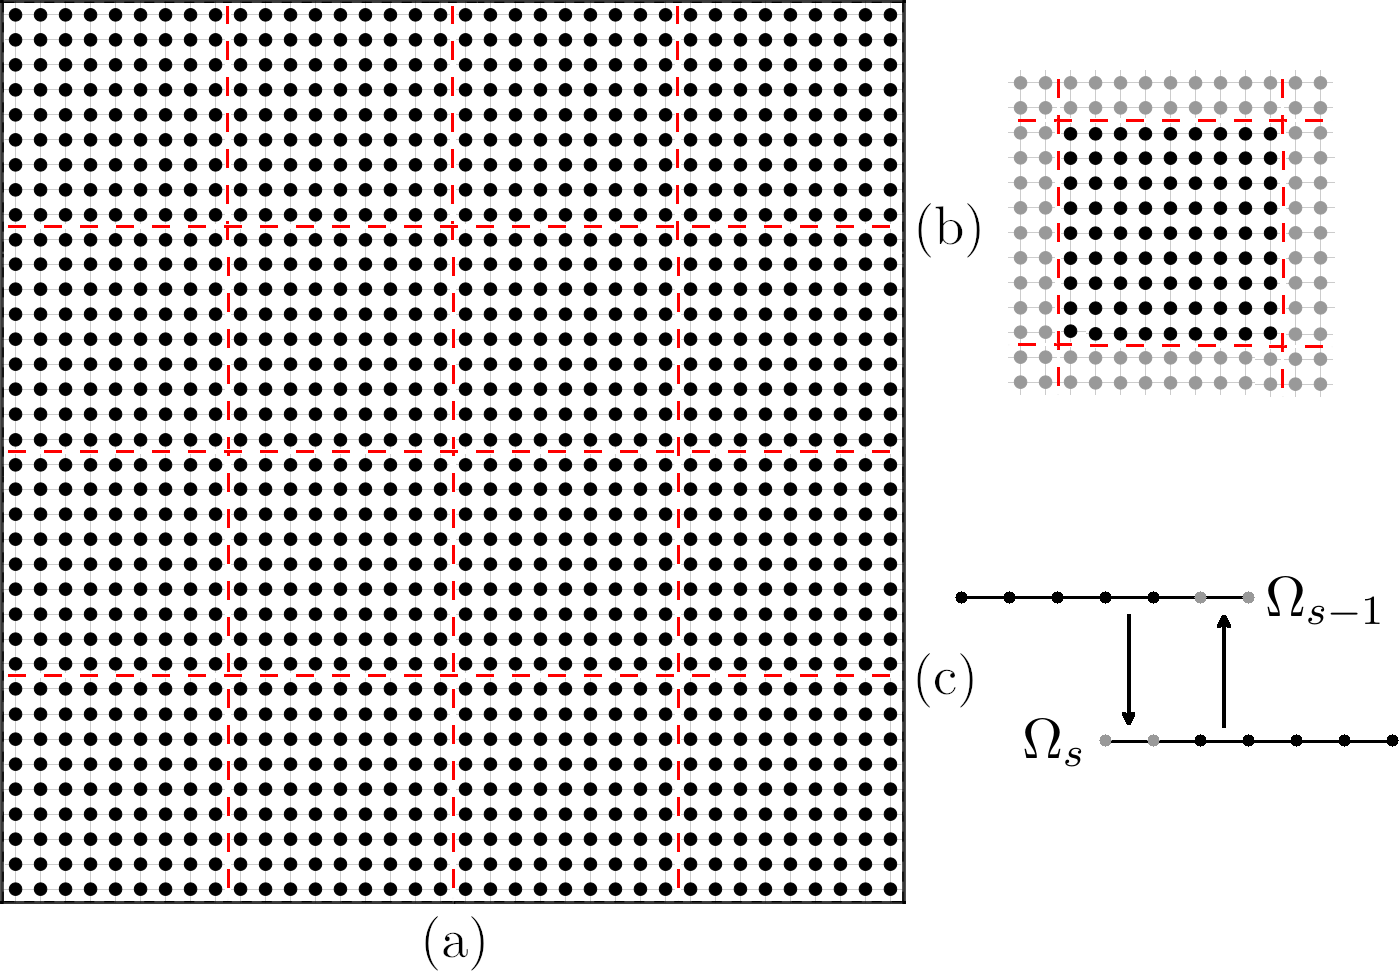
\includegraphics[width=0.6\linewidth]{figuras/all.png}
  \caption{a) El dominio $\Omega$ es dividido en subdominios disjuntos $\widetilde{\Omega}_s$ de modo que 
   $\Omega=\cup_{s=1}^{N_{c}}\widetilde{\Omega}_s$.
   b) Cada subdominio $\widetilde{\Omega}_s$ es extendido  
  en dos puntos (círculos grises) en cada dirección espacial, formando una descomposición en 
  subdominios solapados $\Omega_s$, los cuales se superponen con los subdominios vecinos 
  de forma que $\Omega=\cup_{s=1}^{N_{c}}\Omega_s$. 
  En esta región se recibe información de subdominios vecinos.
   c) Intercambio de información en los bordes de los subdominios solapados 
    $\Omega_s$ y $\Omega_{s-1}$. El 
   procesador $s$ envía a su vecino $s-1$ la información del tercer y cuarto punto de la grilla $s$, y 
   recibe de su vecino los primeros dos puntos.}
 \label{fig:bechange}
\end{figure}

 Cada subdominio contiene un conjunto de puntos  $x_s\in[x_{\text{min},s},x_{\text{max},s}]$ 
 y $y_s\in [y_{\text{min},s},y_{\text{max},s}]$, con los puntos 
 en la grilla dados por $x_i=x_{\min,s}+(i-1)\Delta x$ e $y_j=y_{\min,s}+(j-1)\Delta y$. 
 Definimos  $u_{m}^k(x,y_j)\equiv u_{m,j}^k(x)$ la intensidad específica discretizada a tiempo $t^k$, 
 en la dirección $\hth_m$,
  donde se fijó $y_j\in y_s$ para cualquier $x\in x_s$. 
  Similarmente definimos $u_{m}^k(x_i,y)\equiv u_{m,i}^k(y)$. Al final de cada paso temporal, 
 se realiza el intercambio de puntos entre subdominios vecinos para todos los bordes que no son físicos (bordes 
 originados por la partición), 
 para cada proceso, en cada dirección espacial, y para cada punto de la grilla 
 en esa dirección, como se ilustra en la Figura (\ref{fig:bechange}).

En suma, el algoritmo que resulta de la combinación del método FC con 
el método de ordenadas discretas (D.O.M., del inglés discrete ordinates method), y el método de propagación temporal, 
lo denominamos método FC--DOM~\cite{Gaggioli2019}. El pseudocódigo se presenta en el algoritmo~\eqref{algfc}.
\begin{algorithm}[H]
\caption{FC--DOM en paralelo}\label{algfc}
\begin{algorithmic}[1]
\State  Generar descomposición de dominio
\State Asignar un subdominio $\Omega_s$ a cada procesador.
\State \textbf{para} cada $\Omega_s$ \textbf{hacer} en paralelo
\State \hskip0.5em  Asignar vectores iniciales para el esquema de Adams--Bashforth.
\State \hskip0.5em \textbf{para} cada paso temporal k \textbf{hacer}
\State \hskip0.75em \textbf{para} Cada dirección $\hth_m$ \textbf{hacer} \emph{}
\State \hskip1.0em \textbf{para} cada $y_j$ \textbf{hacer} en la dirección $\hat x$
\State \hskip1.5em Aplicar la continuación de Fourier a $u_{m,j}^k(x)$.
\State \hskip1.5em Aplicar la Transformada Rápida de Fourier para obtener eq.~\eqref{eq:RTEFCSum}.
\State \hskip1.5em Evaluar $\partial u_{m,j}^k(x)/\partial x$ usando la ec.~\eqref{eq:RTEFCSumder}.
\State \hskip1.0em\textbf{terminar}
\State \hskip1.0em\textbf{para} cada $x_i$ \textbf{hacer} en la dirección $\hat y$ 
\State \hskip1.5em Aplicar la continuación de Fourier a $u_{m,i}^k(y)$.
\State \hskip1.5em Aplicar la Transformada Rápida de Fourier para obtener eq.~\eqref{eq:RTEFCSum}.
\State \hskip1.5em Evaluar $\partial u_{m,i}^k(y)/\partial y$ usando ec.~\eqref{eq:RTEFCSumder}.
\State \hskip1.0em\textbf{terminar}
\State \hskip1.0em Evaluar el lado derecho de la ec.~\eqref{eq:RTEAB4}.
\State \hskip1.0em Imponer condiciones de borde.
\State \hskip1.0em Intercambiar bordes no físicos entre subdominios vecinos.
\State \hskip0.75em\textbf{terminar}
\State \hskip0.5em\textbf{terminar}
\State  \textbf{terminar}
\end{algorithmic}
\end{algorithm}
Para realizar un estudio de escalabilidad proponemos un problema típico, 
con  $N=2000$ puntos en cada coordenada espacial $M=16$ direcciones, 
y $T=1000$ pasos temporales. 
Se utilizó un cluster con procesadores Intel Xeon E5-2630 v3 at 2.40GHz de 24 núcleos físicos 
y 128Gb de memoria RAM por nodo. Esta máquina implementa la tecnología ``Intel turbo'', 
que acelera el desempeño del procesador dependiendo de la carga de trabajo y el entorno operativo. 
Para realizar un análisis correcto de escalabilidad, y balancear apropiadamente 
la carga de los nodos, utilizamos 16 procesadores por nodo, 
comparando los tiempos computacionales entre 1 y 16 nodos. 
En la Figura \ref{fig:scala} se observan los tiempos de cómputo 
normalizados $t^*=t/t_{16}$ con respecto al tiempo de cómputo 
en 16 procesadores. 
Como se observa, el algoritmo 
propuesto presenta \textit{escalabilidad paralela perfecta} 
hasta los 256 procesadores para los que fue probado. 
\begin{figure}[h!]
\centering
  \includegraphics[width=0.5\linewidth]{figuras/escalabilidad.eps}
  \caption{Estudio de escalabilidad para problema modelo. 
  Círculos rojos: escalabilidad perfecta, para 256 procesadores $1/t^*=16$. 
  Diamantes negros: Escalabilidad obtenida, $1/t^*=21.872$, dando 
 una eficiencia de $136.7\%$.}
 \label{fig:scala}
\end{figure}

La razón por la cual la escalabilidad obtenida es supralineal se 
desarrolla ampliamente en el trabajo de Albin y Bruno~\cite{Albin2011}
(sección 6). Esencialmente, esto se debe a que el 
las transformaciones FFT 
poseen una complejidad computacional $\mathcal{O}(N\log(N))$.

\section{Validación}

Dado que los algoritmos y los códigos utilizados han sido desarrollados 
originalmente en este trabajo, ha sido necesario realizar exhaustivas 
pruebas de convergencia y validación. Para ello, 
hemos corroborado nuestros resultados tanto con valores experimentales 
como con soluciones analíticas reportadas en la literatura.

\subsection{Convergencia de soluciones manufacturadas}
\label{sec:manufacturada}

Para mostrar las propiedades de convergencia del algoritmo propuesto,
estudiamos un problema manufacturado, analizando el error generado en la propagación de 
la solución.
Con este fin, resolvemos el problema ETR dado por 
\begin{equation*}
\begin{split}
\begin{aligned}
&\frac{1}{c}\frac{\partial }{\partial t}\ut + \hth \cdot \nabla \ut+a(\x)\ut  \\
&\quad \quad \quad  \quad \quad \; \;\,  +b(\x)\ut = \int_{S^1}\eta(\hth\cdot\hth ') 
u(\x,\hat \theta',t) d\theta'+s(\x,\hth,t),  \; (\x,\hth)  \in \Omega\times S^1\\
&u(\x,\hth,t=0)=u_0, \; (\x,\hth)  \in \Omega\times S^1,  \\
&u(\x,\hth,t)=u_b, \; (\x,\hth) \in \Gamma_-. \notag
\end{aligned}
\end{split}
\label{eq:RTEdisp}
\end{equation*}
para $0\leq t \leq T$. 

Proponemos la solución manufacturada
\begin{equation*}
u^{\text{an}}(\x,\hth,t)=e^{-(x-t)^2-(y-t)^2-\cos(\theta)^2}.
\label{eq:RTEmansol}
\end{equation*}
donde el término de la fuente $s(\x,\hth,t)$, 
la condición inicial $u_0(\x,\hth,t)$ y las condiciones 
de contorno $u_b(\x,\hth,t)$ en la ecuación~\eqref{eq:RTEdisp} 
se obtienen, respectivamente, aplicando el operador de transporte, 
evaluando a tiempo $t=0$ y en $\Gamma_-$ la solución manufacturada 
propuesta~\eqref{eq:RTEmansol}.
Resolvemos el problema~\eqref{eq:RTEdisp} en un dominio cuadrado 
$\Omega=\{ \x \in [x_{\text{min}},x_{\text{max}}]\times [y_{\text{min}},y_{\text{max}}] \}$
donde $x_{\text{min}}=y_{\text{min}}=0$ cm, $x_{\text{max}}=y_{\text{max}}=3$ cm, 
y evolucionamos la solución hasta el tiempo final $T=3$ ps. Utilizamos 
una descomposición de 8 subdominios para 
poder realizar estas pruebas en una PC de escritorio. 
El coeficiente de dispersión en el medio considerado es isótropo, 
con $g=0$, $a(\x)=0.35/$cm y $b(\x)=20/$cm. 
%\pagebreak

Evaluamos el error máximo obtenido en todo el dominio 
comparando el flujo escalar dado por la ecuación~\eqref{eq:photondensity} 
obtenido numéricamente comparado con el obtenido analíticamente
\begin{equation*}
\begin{split}
\begin{aligned}
\phi^{\text{an}}(\x,t)&=\int_{2\pi} u^{an}(\x,\theta,t) d\theta=
k_{\phi}\times e^{-(x-t)^2-(y-t)^2},\\
k_{\phi}&=\int_{2\pi}e^{-\cos(\theta)^2}d\theta\simeq 4,052876133898710,
\end{aligned}
\end{split}
\label{eq:photondensityan}
\end{equation*}
y estudiamos las propiedades de convergencia 
para todas las variables involucradas. La constante 
$k_{\phi}$ se calcula con 16 dígitos de precisión. 
La solución numérica es evaluada hasta el tiempo final $T$, 
y luego se calcula el error máximo según\looseness=-1
\begin{wrapfigure}{r}{0.45\textwidth}
 \begin{subfigure}{
  \includegraphics[width=0.45\textwidth]{figuras/errdt.eps}}
 \end{subfigure}
 \begin{subfigure}{
  \includegraphics[width=0.45\textwidth]{figuras/errdx.eps}}
 \end{subfigure}
 \begin{subfigure}{
  \includegraphics[width=0.45\textwidth]{figuras/errdm.eps}}
 \end{subfigure}
  \caption{Convergencia del algoritmo FC--DOM en paralelo 
  para cada una de las variables en la ETR. Las líneas rectas discontinuas 
  muestran la pendiente para un orden de convergencia prescripto. }
 \label{fig:convman}
\end{wrapfigure}
\begin{equation*}
\varepsilon=\text{max}_{\x \in \Omega} |\phi^{\text{num}}(\x,T) -\phi^{\text{an}}(\x,T)|.
\label{eq:maximumerror}
\end{equation*}
El error numérico es en general una función 
de cada una de las variables discretizadas en la ETR, 
\ie~$\varepsilon=\varepsilon(\Delta \x, \Delta \theta, \Delta t)$. 
Al comparar el término del error para una grilla de una dada variable, 
el resto de los parámentros de discretización permanecen fijos.

El alto orden de convergencia del algoritmo FC--DOM en paralelo 
para la solución manufacturada propuesta se muestra en la figura~(\ref{fig:convman}). 
Esta convergencia es la esperada dadas las aproximaciones 
numéricas empleadas.
%\pagebreak 
%\clearpage
\subsection{Comparación con resultados experimentales}
\label{sec:resexp}

En esta sección comparamos los resultados producidos por el algoritmo FC--DOM 
con resultados experimentales obtenidos para varios 
medios similares al tejido humano, realizados por Klose \textit{et al.}~\cite{Klose2002}. 
En las mediciones reportadas en dicha referencia, 
se utilizan fantomas compuestos de resina epoxy y tinta, 
con una concentración de monoesféras de dióxido de silicio ($\text{SiO}_2$). 
La tinta permite ajustar la absorción óptica del fantoma, 
mientras que las monoesféras de silicio determinan su dispersión. 
Las propiedades ópticas del medio (los coeficiente de absorción $a(\x)$
y dispersión $b(\x)$ y el 
factor de anisotropía $g$) han sido determinadas por Klose \textit{et al.} mediante 
diferentes métodos independientes. Estos incluyen simulaciones de Monte--Carlo, 
la técnica de esfera integradora, aproximación de difusión, y teoría de 
dispersión de Mie para ondas electromagnéticas. 

La aproximación de difusión, ampliamente utilizada en tomografía óptica para el 
modelado de transporte de fotones en el tejido biológico, 
es válida para medios de alta dispersión,  
baja absorción y en regiones alejadas de las fuentes.
Dado que nuestro método resuelve el problema ETR completo, podemos considerar adecuadamente 
medios con baja absorción y dispersión, como puede ser el fluido cerebroespinal 
en la cabeza, o la traquea en un cuello humano. 

Analizaremos dos arreglos experimentales diferentes propuestos por Klose~\textit{et al.}. 
Estos poseen simetría 2D, apropiada para nuestro tratamiento. 
 En el primer experimento, se simula un cubo homogéneo, de propiedades ópticas dadas en 
 la Tabla~\ref{tab:tabopt}.
 En el segundo, la geometría del fantoma también 
 es cubica, pero contiene una inhomogeneidad en forma 
 de anillo cilíndrico, con agua en su interior. Esta inhomogeneidad 
 es similar a la que se encuentra en 
 el fluido cerebroespinal, y el fantoma constituye un modelo 
 simple para una cabeza humana. En ambos experimentos,
los fantomas fueron iluminados con luz láser en el 
infrarrojo ($\lambda = 678$ nm), en tres posiciones a lo largo del eje $x$. Se detectó la luz emergente 
en dos de las caras de los fantomas, como se muestra en la figura~(\ref{fig:phantom}).

 
 \begin{table}[h!]
\caption{Propiedades ópticas de los fantomas}
\vspace{-0.6cm}
\begin{center}
\begin{tabular}{cccc}
\hline
$b$ $[cm^{-1}]$ ~~~~~~~~ & $a$ $[cm^{-1}]$ & ~~~~~~~~ $g$  ~~~~~~~~ & $n_{\Omega}$ \\
\hline
58 ~~~~~~~~ & 0.35 & ~~~~~~~~  0.8 ~~~~~~~~ & 1.56 \\
\hline
\end{tabular}
\label{tab:tabopt}
\end{center}
\end{table}

\begin{figure}[h!]
\centering
  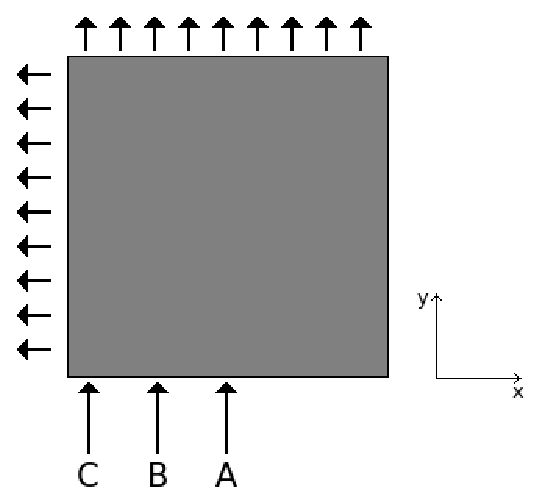
\includegraphics[width=0.4\linewidth]{figuras/phantom.eps}
   \caption{Arreglo experimental de Klose \textit{et al.}~\cite{Klose2002}. 
   Las flechas apuntando hacia el fantoma (A, B y C)  
   muestran las tres posiciones diferentes en las que se inyectó 
   la luz láser. Las flechas salientes muestran las posiciones de los detectores 
   con las que se midió la radiación saliente.}
 \label{fig:phantom}
\end{figure}

El método de continuación de Fourier extiende 
la intensidad específica en el borde del dominio, 
permitiendo el tratamiento de condiciones de borde generales y no periódicas.  
Esto previene el surgimiento del fenómeno de Gibbs debido a la no periodicidad 
de la función. La fuente $q(\x,\hth,t)$ y los parámetros ópticos 
también pueden dar origen al fenómeno de Gibbs si no son 
tratados correctamente. Los problemas numéricos que surgen 
debido a discontinuidades son resueltos mediante aproximaciones arbitrariamente precisas 
introduciendo funciones suaves que presentan 
variaciones rápidas en la región de discontinuidad (en conjunto 
con discretizaciones capaces de resolver dichas variaciones).

Dado que nuestro algoritmo resuelve el problema ETR dependiente del tiempo, 
y que los resultados experimentales reportados por Klose \textit{et al.} 
son independientes del tiempo, evaluaremos la corriente de fotones saliente 
\begin{equation}
 \vec{ \mathcal{J}}_+(\x,t)=\int_{\Gamma_+} [1-f(\hth \cdot \hnu)] \hth \cdot \hnu u(\x,\hth,t) d\theta,
\label{eq:photoncurrentsal}
\end{equation}
utilizando una función sigmoidea para el perfil temporal, $T(t)$, 
que adquiere suavemente valores partiendo desde cero 
hasta uno. La solución independiente del tiempo 
se adquiere a un tiempo asintótico.
La fuente láser se modela por la función
\begin{equation}
q(\x,\hth,t)=T(t)\exp \left(  -\frac{|\x-\x_s|^2}{2\sigma^2} \right)  \, ,
\label{eq:sourceGauss}
\end{equation}
donde el valor de $\sigma=0.1$ cm es el reportado para el experimento y $\x_s$ 
representa la posición del láser. La información direccional de la fuente 
puede ser muy valiosa en diversos tipos de experimentos. 
En el caso particular que analizamos, el medio es altamente dispersivo. Por lo tanto, los 
fotones pierden rápidamente esta información 
luego de atravesar una corta distancia (del orden del camino libre medio).

Se resuelve la ETR para un número de pasos temporales, 
hasta que la solución alcanza, numéricamente, el comportamiento 
asintótico~\cite{Bruno2010}, para el cual $\lim_{t\to \infty} \frac{\partial u}{\partial t}=0$. 
Luego se evalúa el operador de la ecuación~\eqref{eq:photoncurrentsal} 
en las regiones de la superficie en $\partial \Omega$ 
donde se ubican los detectores.
Una vez  calculada la corriente de fotones salientes, se
se realiza una normalización para ubicar la lectura 
de los resultados experimentales (reportados en escala arbitraria) 
en la misma escala que las obtenidas por el método FC--DOM. 
Para las detecciones a lo largo del eje $x$ se normalizó 
con respecto al máximo valor de cada curva. 
 Las lecturas de los detectores sobre el eje $y$ 
 se normalizaron ajustando el punto en la grilla numérica 
 que se encontró mas cerca de la posición reportada 
 para alguno de los detectores. 
 
\subsubsection{Fantoma homogéneo}

El primer arreglo experimental reportado por~\cite{Klose2002} 
se basa en un fantoma homogéneo con los parámetros ópticos 
dados en la tabla~\ref{tab:tabopt}. El fantoma posee un tamaño  
de $3$ cm a lo largo de los ejes $x$ e $y$. La posición del láser 
   $\x_s$ es, para los tres casos considerados $A=(1.5,0)$ cm, $B=(0.9,0)$ cm
    y $C=(0.3,0)$ cm. En la figura~(\ref{fig:ph1timef}) se muestra 
el flujo escalar~\eqref{eq:photondensity} 
correspondiente a las tres posiciones de la fuente láser $\x_s$. 

\begin{figure}[h!]
\centering
  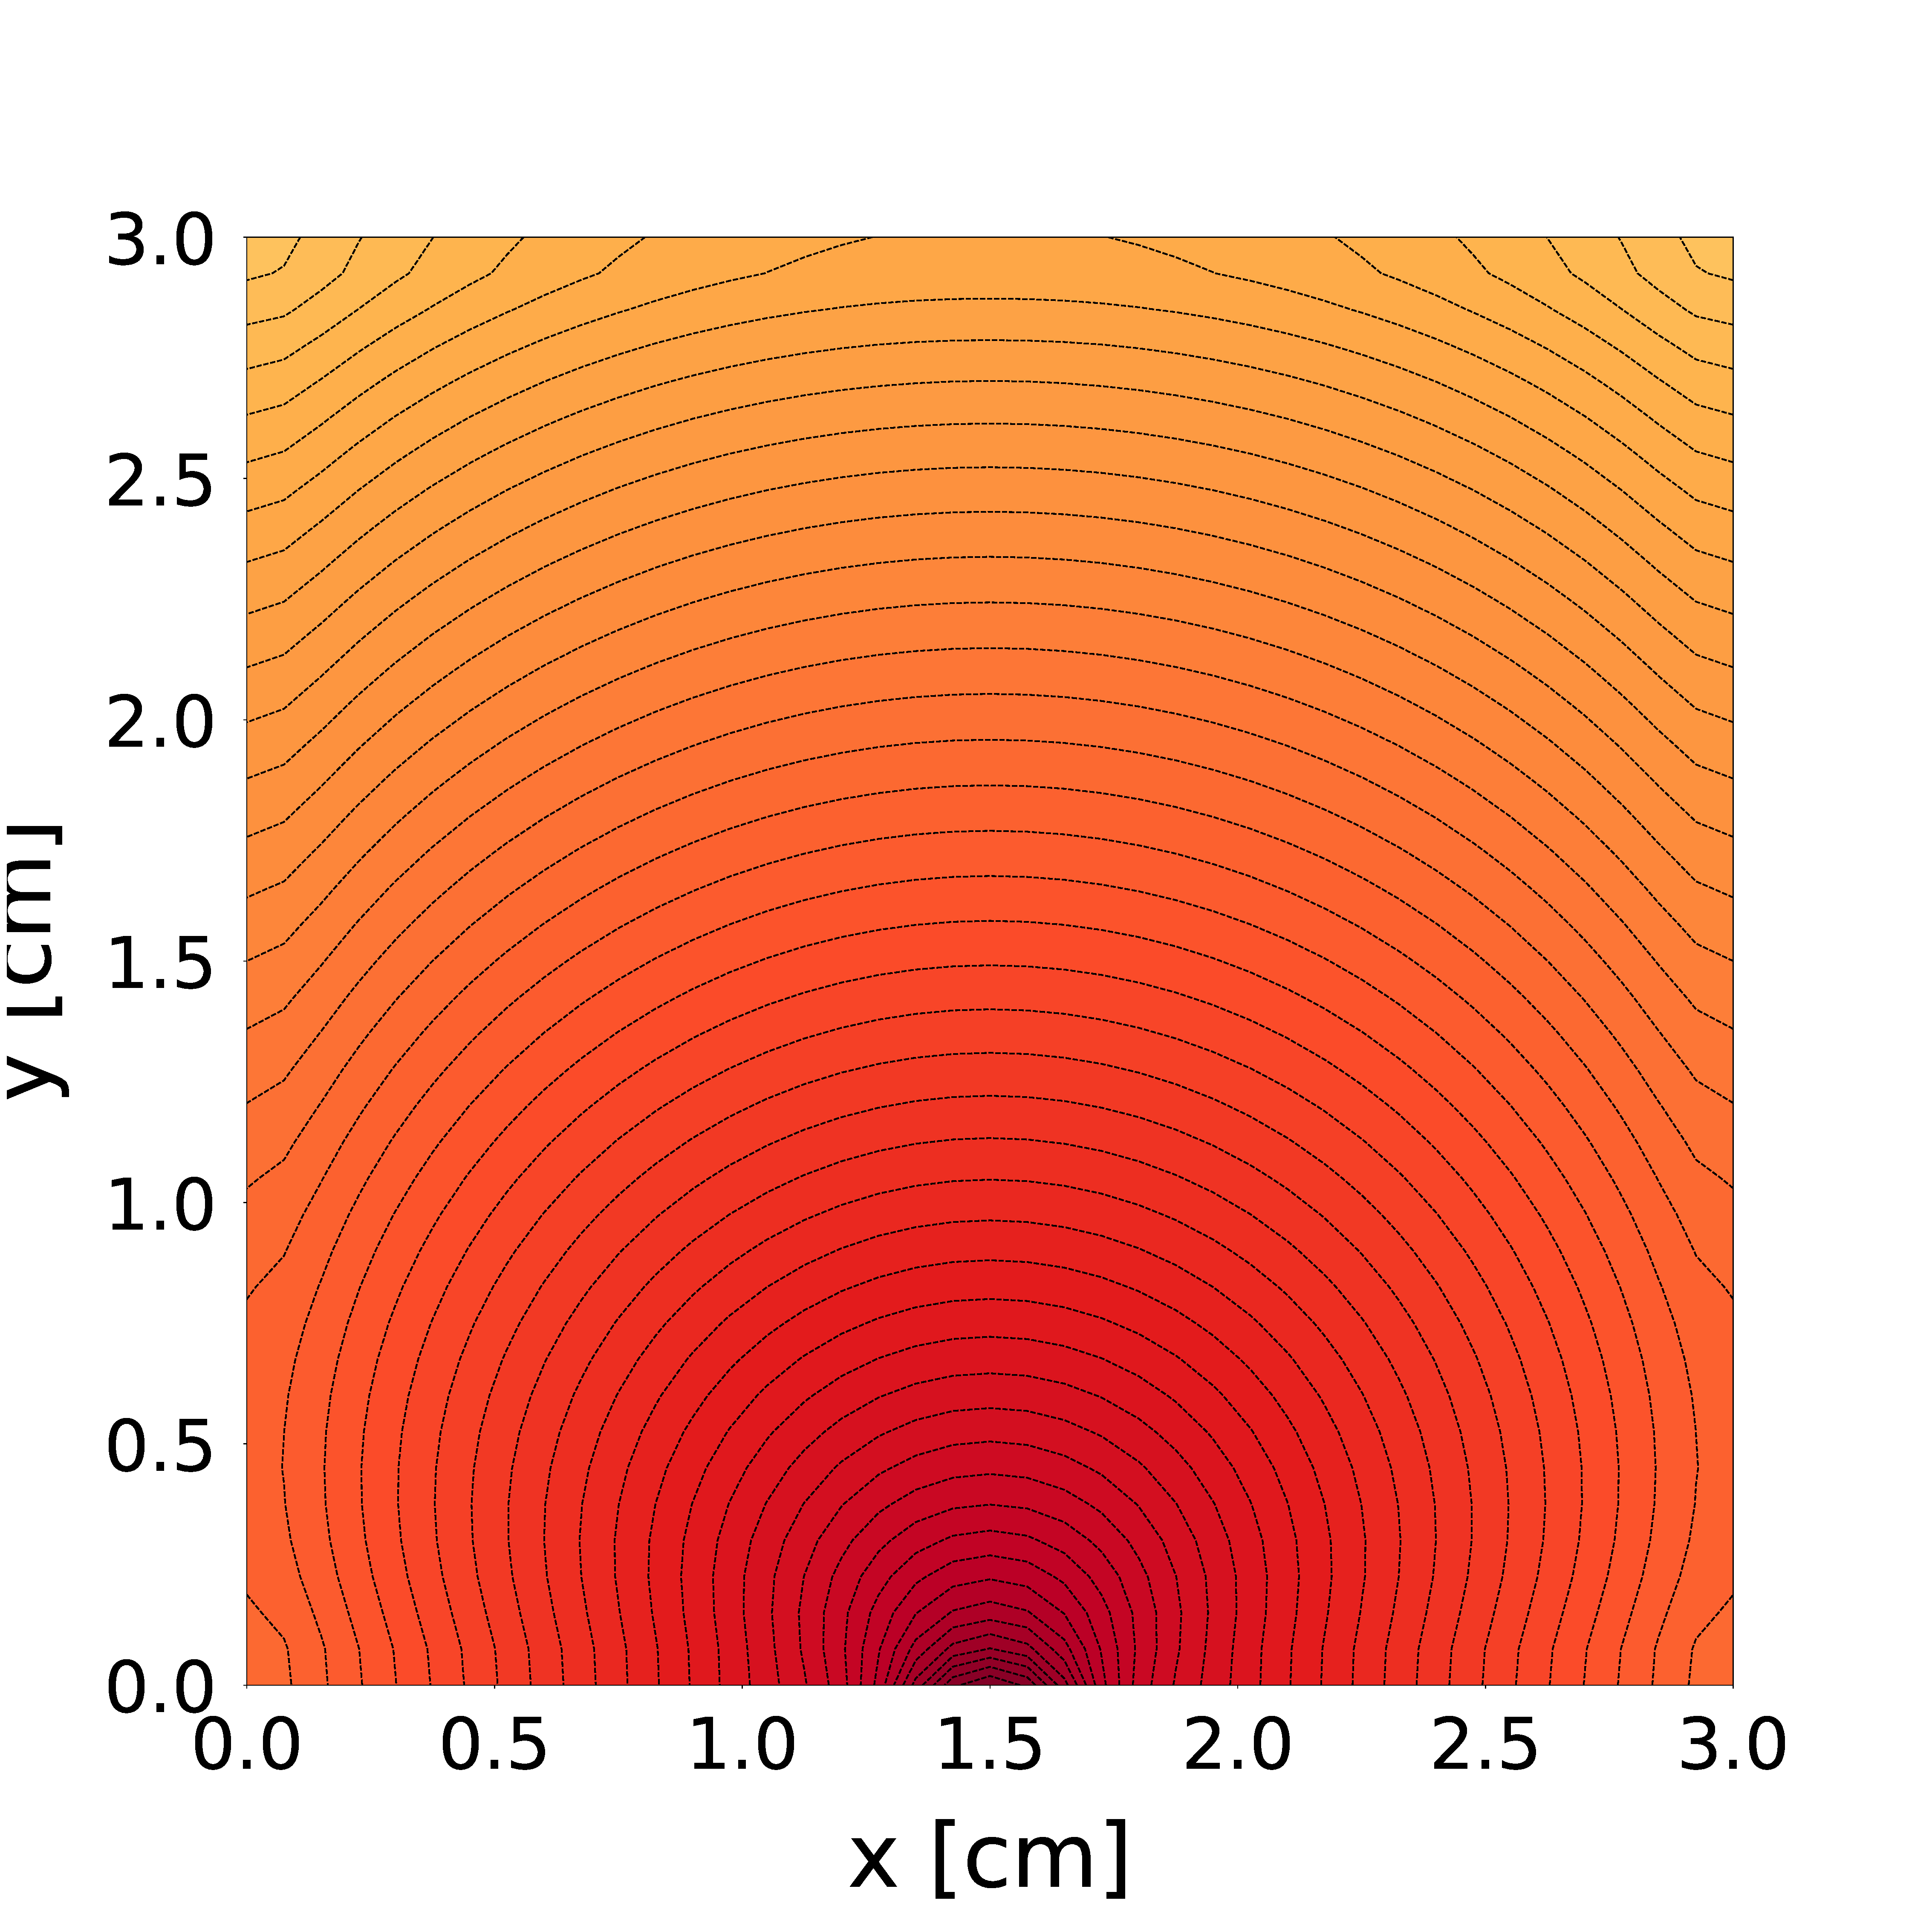
\includegraphics[width=0.32\linewidth]{figuras/ph1A.eps}
  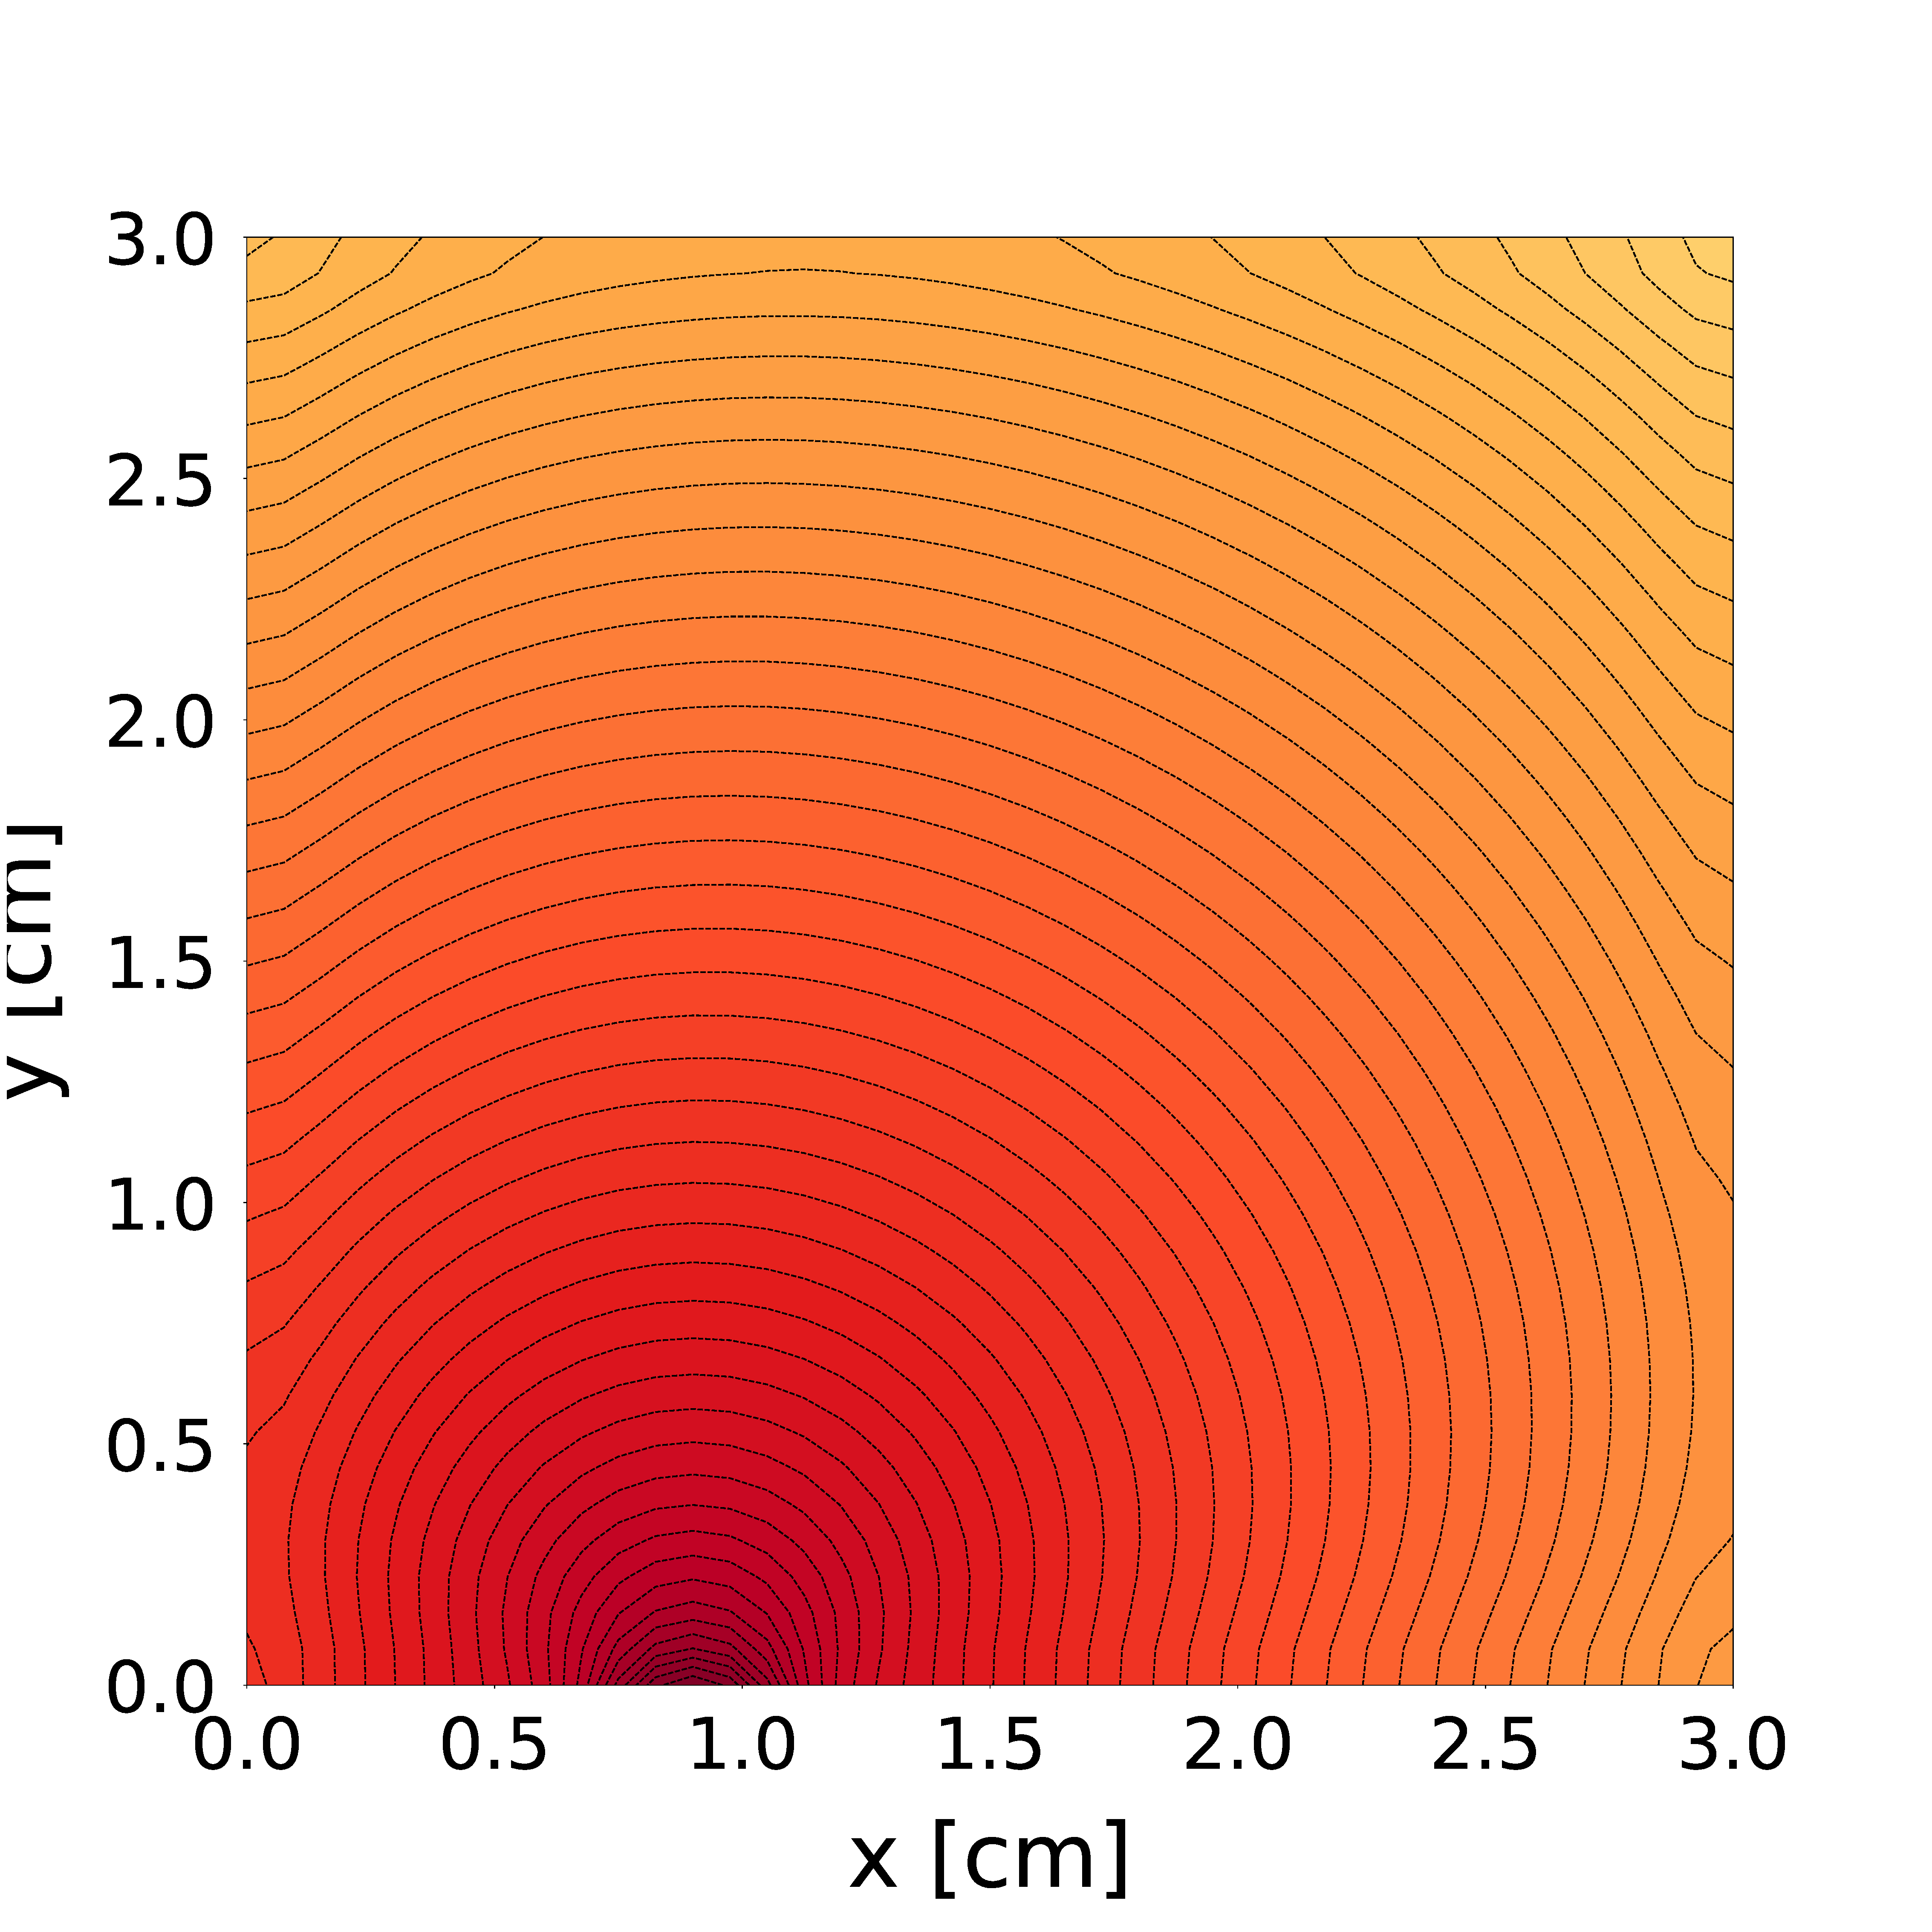
\includegraphics[width=0.32\linewidth]{figuras/ph1B.eps}
  
\includegraphics[width=0.32\linewidth]{figuras/ph1C.eps}
  \caption{
  Flujo escalar $\phi(\x)$~\eqref{eq:photondensity} 
  obtenido en la simulación para el fantoma homogéneo. 
  Las tres figuras muestran los resultados obtenidos 
  para las fuentes ubicadas en A (izquierda), B (centro) y C (derecha). 
  Debido al decaimiento exponencial inherente a la solución, 
  la figura se presenta en escala logarítmica para apreciar los detalles.}
\label{fig:ph1timef}
\end{figure}
Como puede apreciarse en la figura, el flujo escalar para el caso A 
es simétrico con respecto al eje vertical situado en la posición 
de la fuente, pero el sistema pierde esta propiedad cuando la 
posición de la fuente se ubica más cerca de los bordes, 
dando lugar a reflexiones que afectan la intensidad 
de la luz con una dependencia angular particular.

El flujo de fotones que llegan a los detectores, ubicados en el borde $\partial \Omega$ 
del dominio, se obtuvo mediante la ecuación~\eqref{eq:photoncurrentsal}. 
Los resultados se muestran en la Figura~(\ref{fig:fluxph1}), 
para los 28 detectores ubicados en el borde a lo largo del eje $x$ (izquierda) 
y para los 28 detectores en la dirección $y$ a la derecha. 
Se observa un acuerdo excelente entre los resultados simulados (líneas) 
y los datos experimentales (en símbolos).  El máximo 
flujo de fotones salientes $\mathcal{J}_+$ en los experimentos B, 
y particularmente en el C, se encuentran desviados con respecto a la posición 
de la fuente láser. Esto puede explicarse considerando la radiación 
que está siendo reflejada y que escapa a través de la superficie de la izquierda. 
A medida que la fuente se acerca más al borde, el ángulo de incidencia de la 
radiación con respecto a la normal de la superficie aumenta. Por lo tanto, 
más radiación resulta reflejada desde puntos cercanos a la superficie, 
propagandose hacia el interior del medio participante, 
contribuyendo al máximo. También se espera que la contribución de fotones dispersados 
por el medio desde la región a la derecha sea relativamente mayor 
que desde la izquierda, ya que la radiación 
dispersada en esta última tiende a escapar por el borde. 
\begin{figure}[h!]
\centering
  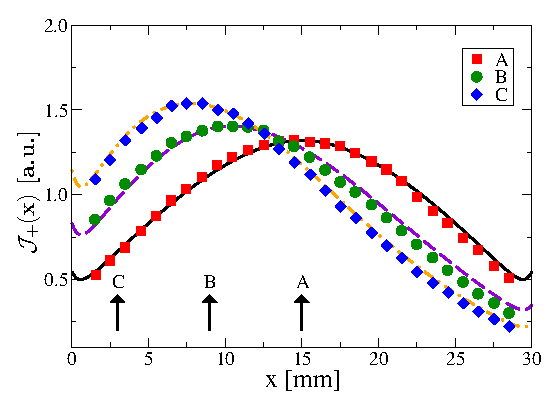
\includegraphics[width=0.48\linewidth]{figuras/kloseph1x.eps}
  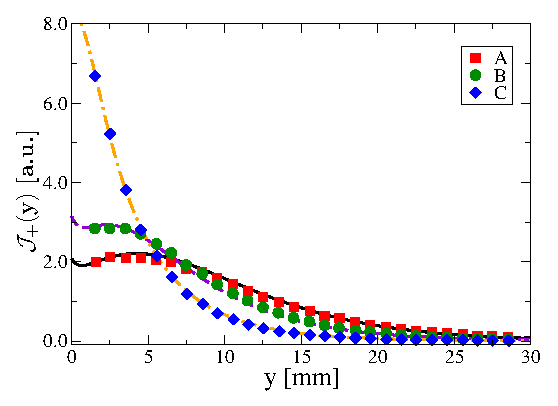
\includegraphics[width=0.48\linewidth]{figuras/ph1y.eps}
  \caption{Radiación transmitida medida por Klose~\cite{Klose2002} (símbolos), 
  y simulada mediante el método FC--DOM (lineas) para el fantoma homogéneo. }
 \label{fig:fluxph1}
\end{figure}
También puede observarse un aumento en el flujo de fotones en la región más 
cercana al borde, proveniente de fotones que han sufrido reflexión total interna.

Este experimento también fue simulado y analizado por Klose {\it et al.}~\cite{Klose2002}
en el marco de la teoría ETR independiente del tiempo.

\subsubsection{Fantoma inhomogéneo}

El segundo fantoma contiene una región de ``vacío'' en forma de anillo, 
rellena de agua, de diámetro $d=2,8$ cm, en donde el coeficiente de absorción 
y dispersión están dados por $a(\x)=b(\x)=0$. En el resto del medio, 
se consideran los parámetros ópticos de la tabla~\ref{tab:tabopt}
Las dimensiones de este fantoma a lo largo del eje $x$ e $y$ es de $4$ cm.
Se realizaron simulaciones para tres experimentos, de acuerdo a las posiciones 
$\x_s$ de la fuente $A=(2.0,0)$ cm, $B=(1.2,0)$ cm, 
y $C=(0.4,0)$ cm.
Para evitar el deterioro de la convergencia del método, las discontinuidades
 en los parámetros ópticos del medio 
deben ser evitadas. De otra forma, el fenómeno de Gibbs deterioraría 
la precisión de los cálculos. Por esta razón, implementamos una aproximación 
suave a los coeficientes, haciendo uso de la función ventana introducida 
por Bruno \textit{et al}.~\cite{Bruno2014a} en otro contexto. 
Esta función provee una transición suave hacia la región de 
vacío.
En la figura~(\ref{fig:scattcoef}), se muestra una representación de los 
parámetros ópticos utilizados para el fantoma inhomogéneo, 
donde puede observarse la transición suave a la inhomogeneidad 
en forma de anillo.
 \begin{figure}[h!]
\centering
  
\includegraphics[width=0.35\linewidth]{figuras/sigs.eps}
  \caption{Coeficiente de dispersión para el fantoma inhomogeneo, 
  con región de vacío en forma de anillo donde  $a(\x)=b(\x)=0$.}
 \label{fig:scattcoef}
\end{figure}
El flujo escalar para el fantoma inhomogéneo se muestra en la Fig.~(\ref{fig:ph2timef}). 
\begin{figure}[h!]
\centering
  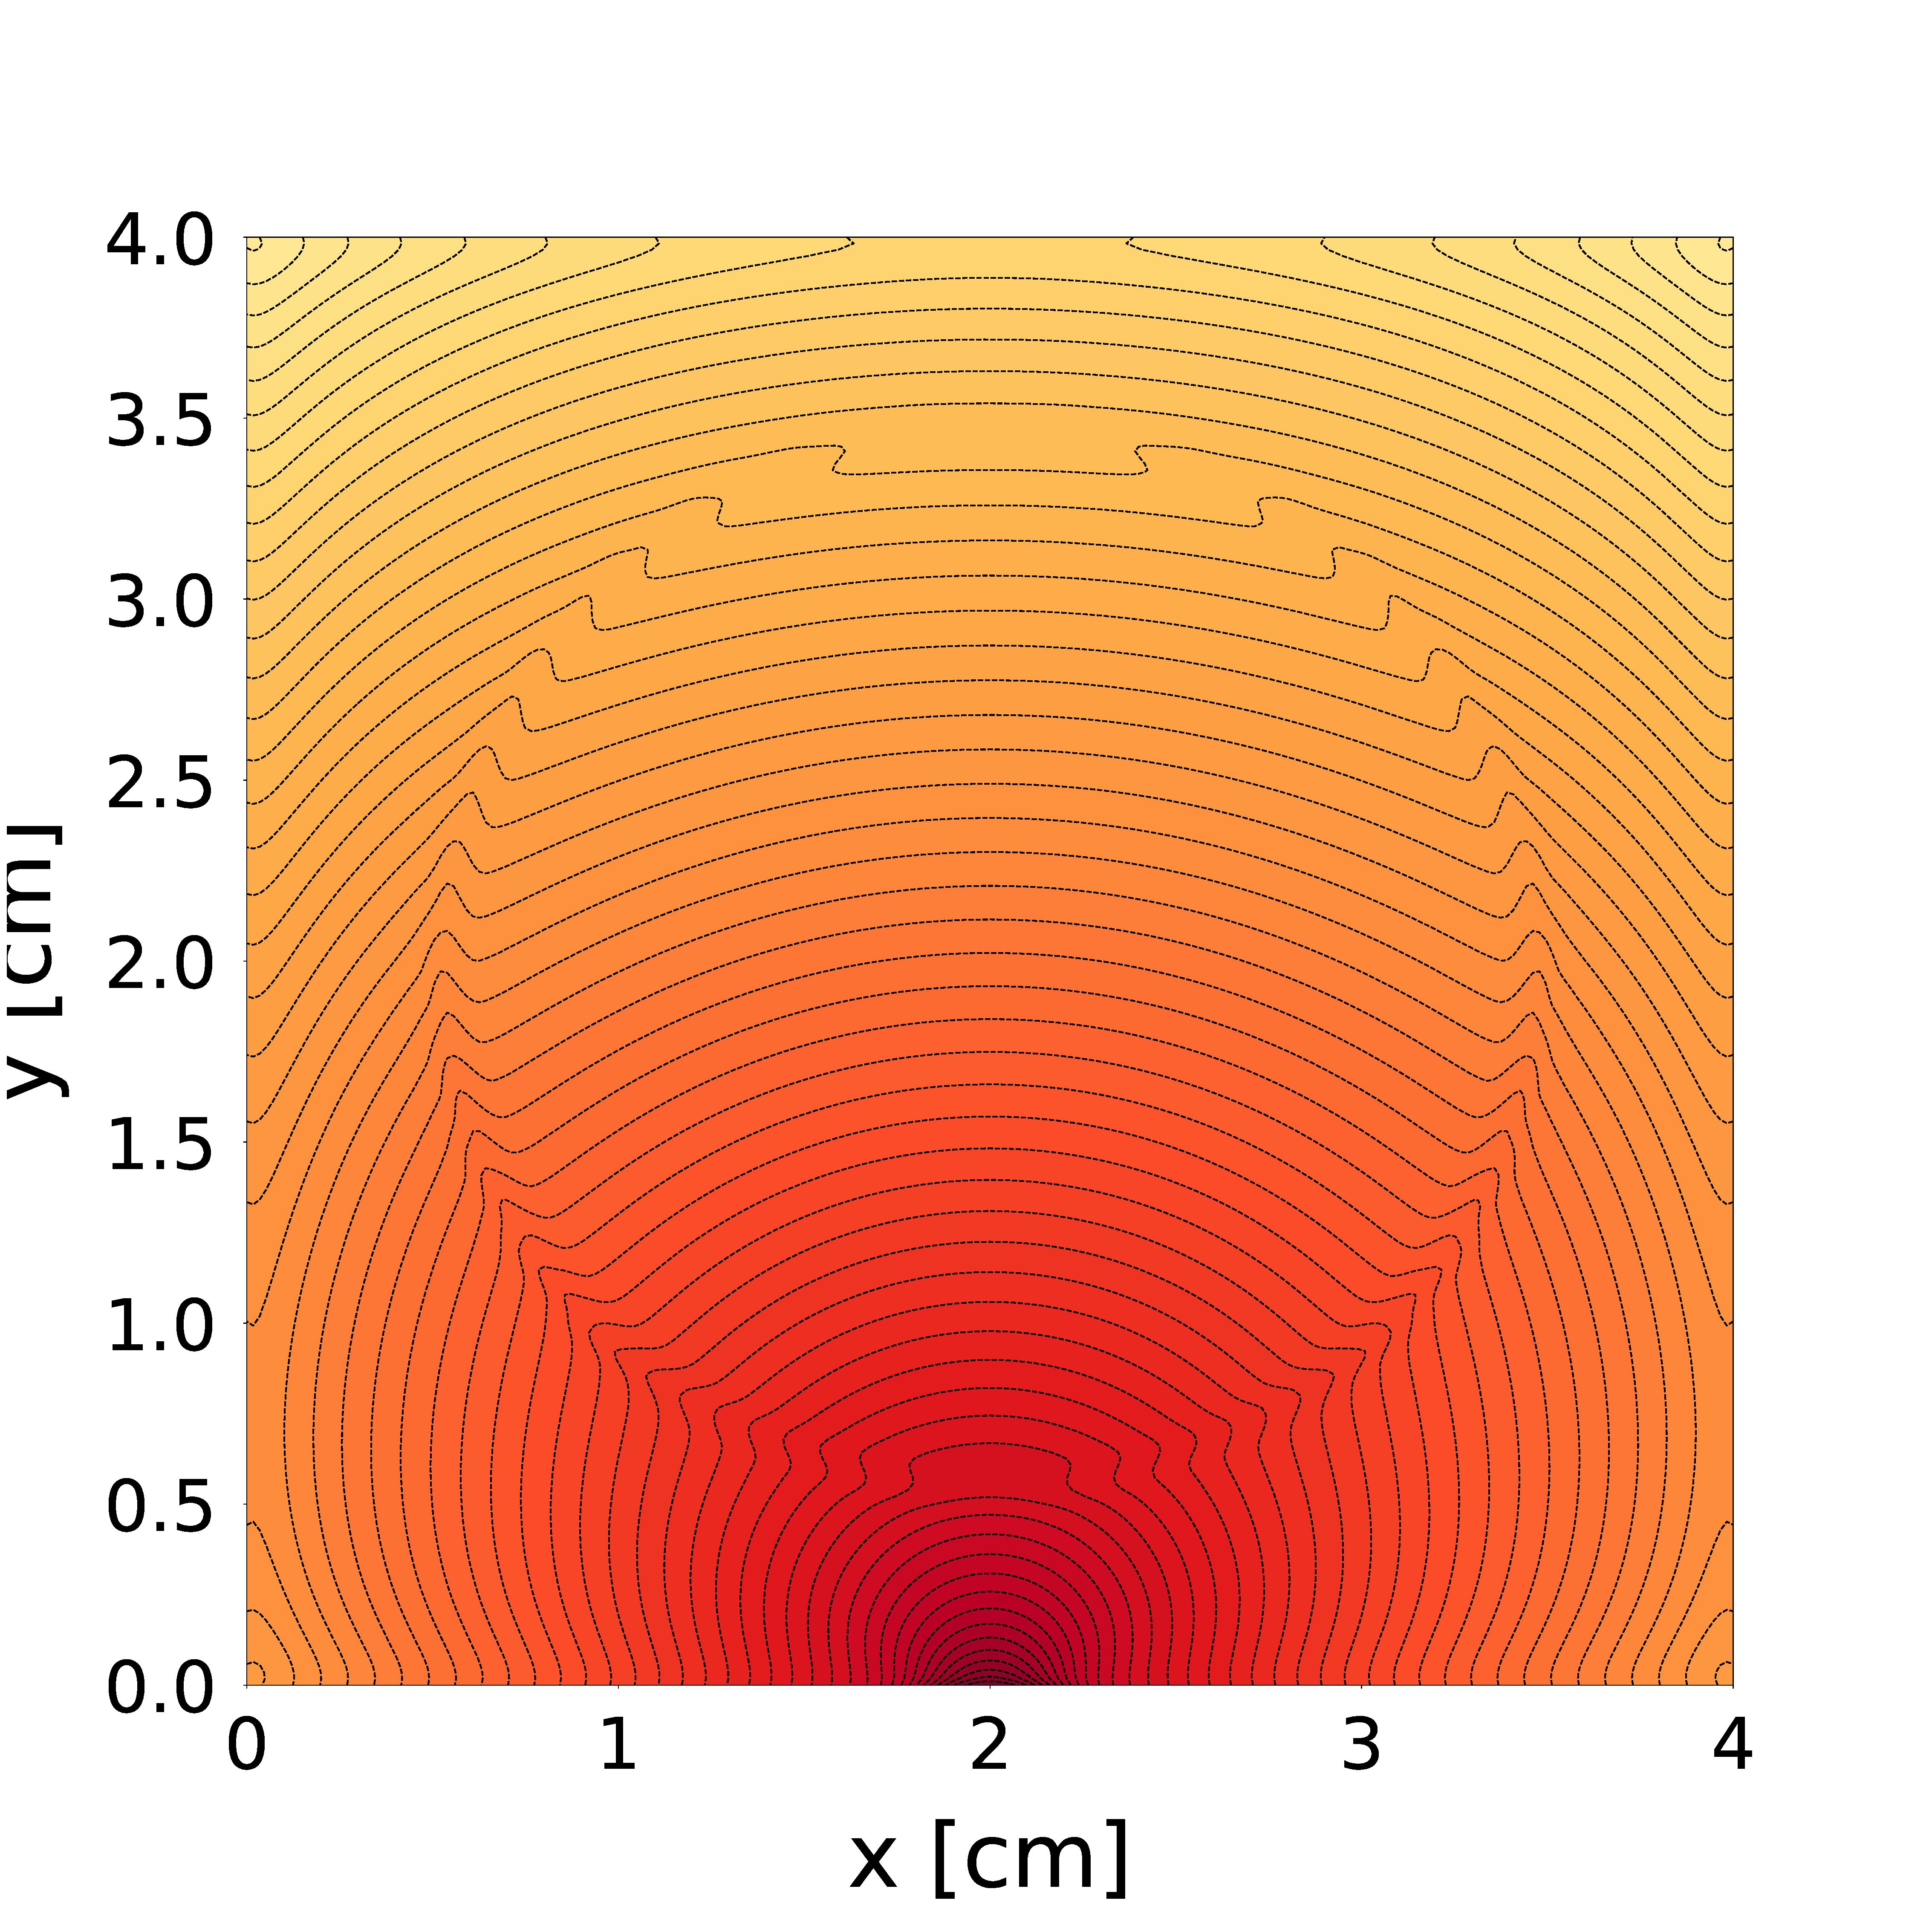
\includegraphics[width=0.32\linewidth]{figuras/ph2A.eps}
  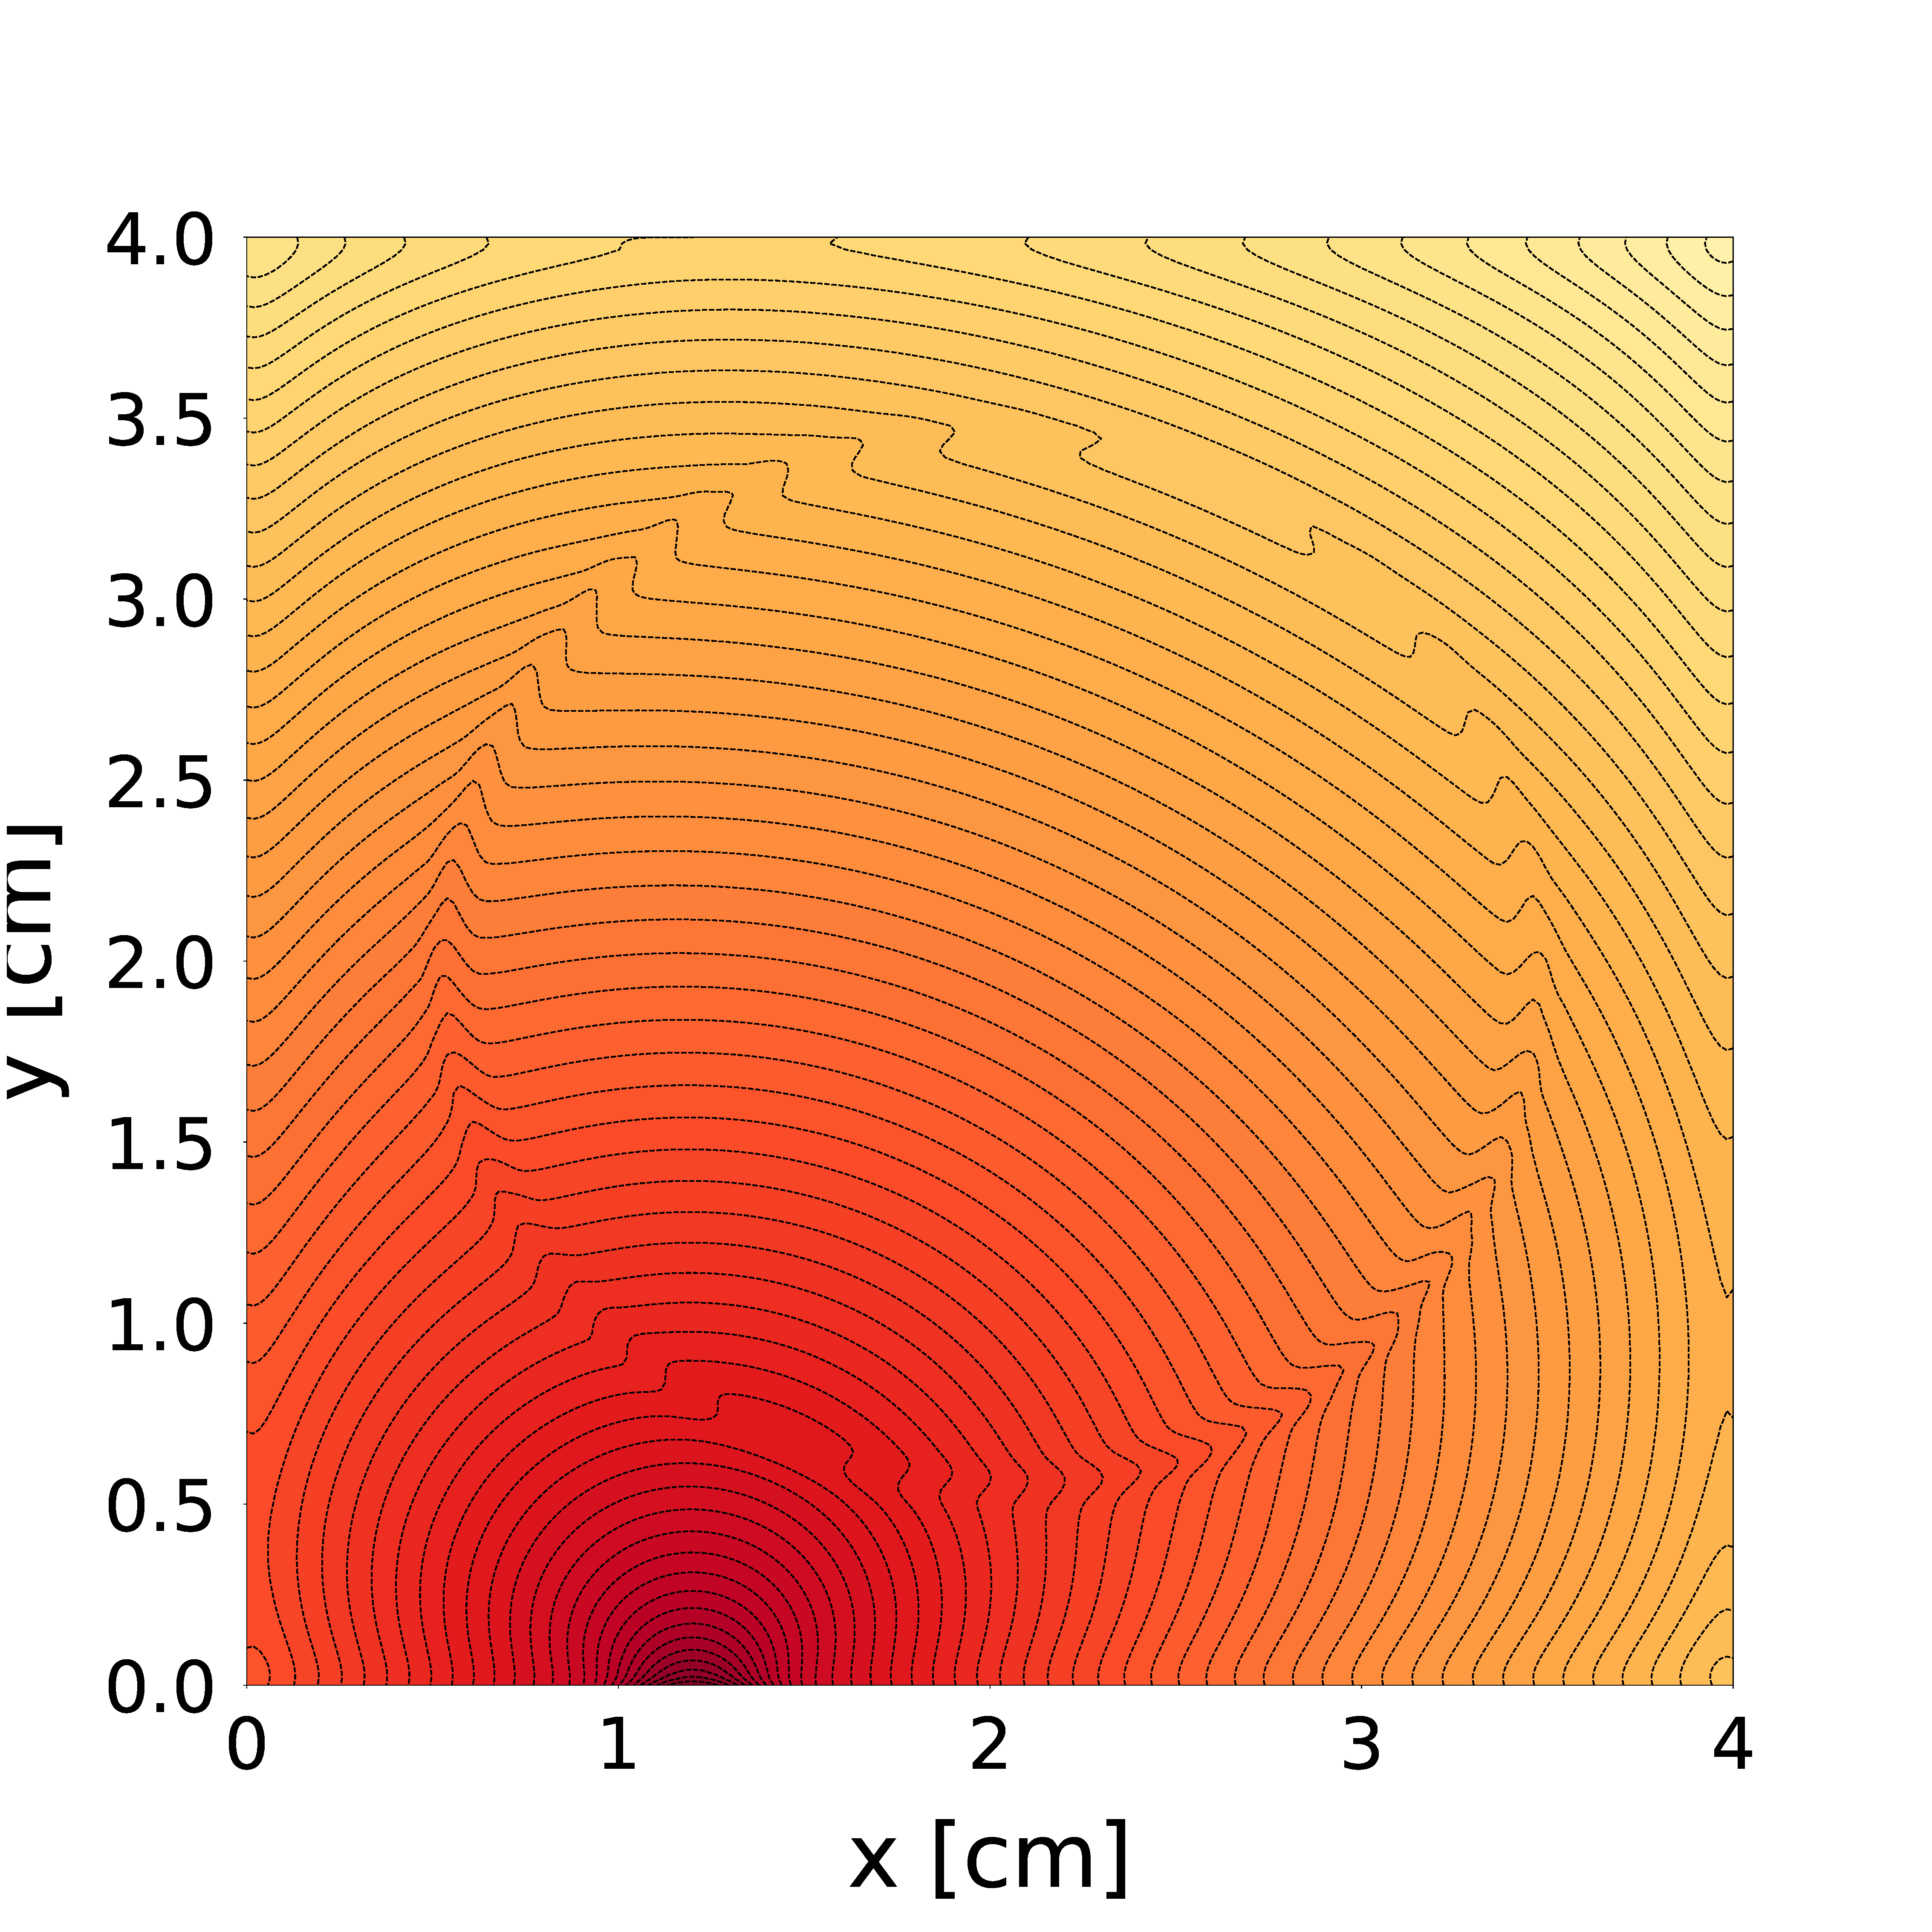
\includegraphics[width=0.32\linewidth]{figuras/ph2B.eps}
  
\includegraphics[width=0.32\linewidth]{figuras/ph2C.eps}
  \caption{Flujo escalar $\phi(\x)$~\eqref{eq:photondensity} 
  obtenido en las simulaciones para el fantoma inhomogéneo. A (izquierda), B (centro) y C (derecha).}
 \label{fig:ph2timef}
\end{figure}
Estos resultados muestran claramente el efecto de la región de vacío. 
En esta región, los fotones viajan libremente. Esta característica 
implica que este problema no puede ser correctamente resuelto 
mediante la aproximación de difusión.
El flujo de fotones que llegan a los 38 detectores ubicados en la frontera del 
dominio se muestra en la figura~(\ref{fig:fluxph2}). 
Se observa un buen acuerdo entre teoría y experimento, aunque 
con mayores desviaciones respecto al caso del fantoma homogéneo. 
Estas desviaciones pueden explicarse por el hecho de que 
en nuestras simulaciones no estamos teniendo en cuenta la reflexión 
de Fresnel que ocurre en la interface del anillo cilíndrico, 
lo cual requeriría de un tratamiento especial~\cite{Bal2006}. 

La presencia de regiones de vacío, como la que se encuentra en el 
fluido cerebroespinal en la cabeza, o entre órganos en el cuerpo 
--el fluido sinovial en las articulaciones~\cite{Netz2001}, 
o la traquea en el cuello humano~\cite{Fujii2016}--, 
requiere del uso de la ETR como modelo físico, ya que la 
aproximación de difusión de fotones no es apropiada en este régimen de transporte. 
\begin{figure}[h!]
\centering
  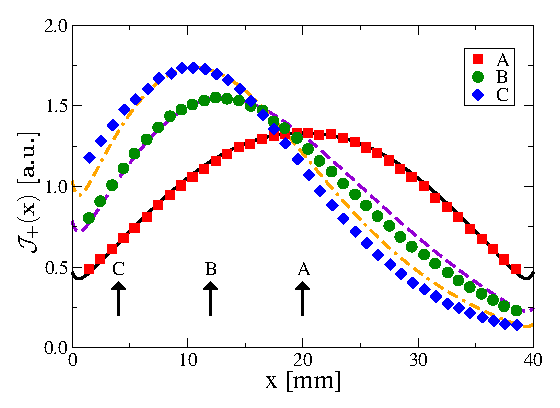
\includegraphics[width=0.48\linewidth]{figuras/kloseph2x.eps}
  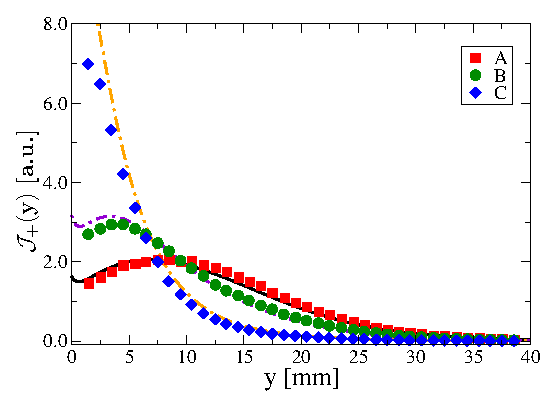
\includegraphics[width=0.48\linewidth]{figuras/ph2y.eps}
  \caption{Radiación transmitida medida por Klose~\cite{Klose2002} (símbolos),
  y radiación obtenida mediante las simulaciones FC--DOM, para 
  el fantoma inhomogéneo (líneas).}
 \label{fig:fluxph2}
\end{figure}
Tanto este experimento como el previo, han sido simulados por Klose {\it et al.} 
\cite{Klose2002} mediante el uso de diferencias finitas, utilizando la ETR 
independiente del tiempo.

\subsection{El fenómeno de rayos}
\label{subsec:rayeff}
En esta sección presentamos el último caso independiente del tiempo 
que trataremos en esta tesis. Este concierne a un 
fenómeno importante que surge en las aproximaciones numéricas 
que utilizan métodos de ordenadas discretas para resolver la ETR~\cite{Lewis1984}. 
Se trata del fenómeno de rayos, 
el cual se manifiesta esencialmente en medios de baja dispersión. 
El fenómeno de rayos se origina debido a la discretización 
de la variable angular $\hth$. Debido a dicha discretización, 
las direcciones posibles para la propagación de los fotones 
se encuentra limitada. Cuando existen fuentes localizadas, 
se originan variaciones rápidas en la intensidad específica 
cerca de estas. La propagación del flujo queda restringida 
en las direcciones discretas, dando origen a oscilaciones 
espurias, conocidas como efecto de rayos. 

Analizamos un problema  
de referencia ampliamente utilizado, 
diseñado específicamente para estudiar este efecto numérico.
Dadas las dimensiones del mismo, 
los fotones no llegarán a sufrir suficientes eventos de colisión.
Reproducimos 
el caso reportado por Crosbie y Schrenker~\cite{Crosbie1984}, 
el cual proporciona flujos considerados exactos~\cite{Ramankutty1997,tagnekamdem2015}, 
utilizando el método FC--DOM para soluciones independientes 
del tiempo obtenidas por relajación del caso dependiente del tiempo. 

Consideramos un dominio bidimensional cuadrado, de lado unitario, 
que contiene un medio puramente dispersivo (sin absorción) 
con $b(\x)=1$. La dispersión considerada es isótropa ($g=0$). 
La radiación incide de manera uniforme sobre la superficie inferior del medio. 
El resto de los bordes presentan condiciones de contorno de vacío ($n_{\Omega}=n_{s}$ 
de donde $f(\hth \cdot \hnu)=0$). El observable considerado es la componente en
 $y$ de la corriente de fotones~\eqref{eq:photoncurrent} $\mathcal{J}_y(x,y=1)$. En la Figura~(\ref{fig:fluxph3}) 
se presentan los resultados obtenidos (líneas), y los valores de referencia (símbolos). 
Se observa que el efecto de rayos se manifiesta en discretizaciones 
relativamente gruesas de la variable angular, y disminuye al aumentar 
el número de direcciones. 
El método de continuación de Fourier sólo trata 
al operador diferencial en las variables espaciales, independientemente 
de la discretización angular. Por lo tanto, no 
resuelve el fenómeno de rayos y otras estrategias deben ser consideradas 
para solucionarlo.
\begin{figure}[h!]
\centering
  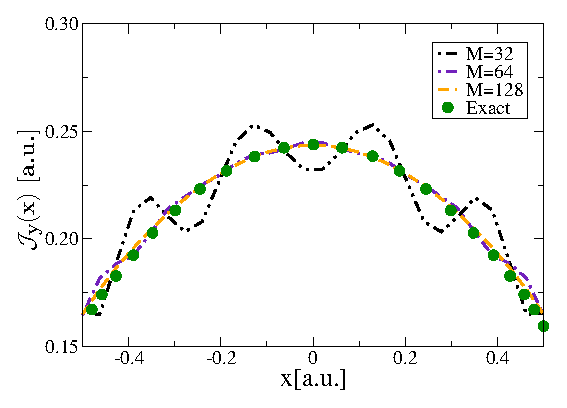
\includegraphics[width=0.48\linewidth]{figuras/raycurrent.eps}\\
  \caption{
Círculos: corriente de fotones exacta en la dirección $y$, $\mathcal{J}_y(x)$. 
Líneas: valores simulados obtenidos por el método FC--DOM, 
para un número variable de direcciones: $M=32,64,128$. El gráfico 
se presenta en unidades arbitrarias (a.u).}
 \label{fig:fluxph3}
\end{figure}

En medios altamente dispersivos, el comportamiento singular 
que origina el fenómeno de rayos resulta rápidamente atenuado lejos 
de la fuente, debido a que la radiación directa 
(los fotones balísticos que no han sufrido dispersión) decaen rápidamente
~\cite{Ramankutty1997}, redistribuyendo la radiación en todas las 
direcciones. Este fenómeno no suele ser un problema en tejidos biológicos, 
ya que estos son altamente dispersivos.

\subsection{Comparación con solución analítica}

En esta sección validamos nuestros métodos computacionales 
dependientes del tiempo calculando el flujo escalar, 
y comparándolo con la solución analítica dada por Paasschens~\cite{Paasschens1997} 
para una fuente puntual en un medio infinito. 
En este problema, un medio bidimensional infinito, 
isótropo y homogéneo es iluminado por una fuente puntual isótropa
ubicada en el origen de coordenadas $s(\x,\hth,t)=\delta(\x)\delta(t)$.

El flujo escalar resultante en este caso es 
\begin{equation}
\begin{split}
\begin{aligned}
\phi(r,t)=\frac{e^{-c t \, (a+b')}}{2\pi}\delta(ct-r)&+\frac{b'}{2\pi c t}\left(1-\frac{r^2}{c^2t^2}\right)^{-1/2}\\
&\times\exp\left[b'\sqrt{c^2t^2-r^2}-c t \, (a+b')\right]H(ct-r),
\end{aligned}
\end{split}
\label{eq:Paasschenssc}
\end{equation}
donde $H(x)$ es la función escalón de Heaviside, 
y se ha hecho uso del coeficiente de dispersión reducido $b'=(1-g)b$, 
el cual aproxima la anisotropía en la dispersión.
Para esta simulación empleamos un fantoma homogéneo con las propiedades ópticas 
dadas en la Tabla~\ref{tab:tabopt}, de donde $c=0.019$ cm/ps, 
utilizando el coeficiente de dispersión reducido con $g=0.8$, y función de fase isótropa (con $g=0$ en la Ec.~\eqref{eq:Henyey-Greeinstein}). 


El primer término en la expresión~\eqref{eq:Paasschenssc} 
representa el pico balístico~\cite{Paasschens1997}, originado 
por los fotones que no han sufrido dispersión, y que arriban a una distancia $r$
 de la fuente en un tiempo $t=r/c$.
En el caso de medios altamente dispersivos, este término resulta rápidamente atenuado 
a unos pocos milímetros de la fuente. Para las simulaciones numéricas 
empleamos condiciones de borde de vacío, en las cuales el flujo 
entrante a través de la superficie del dominio $\partial \Omega$ es nulo 
\begin{equation}
u(\x,\hth,t)=0 \;\;\; \text{en}\; \Gamma_{-} \, .
\label{eq:vacuumbc}
\end{equation}
A los efectos prácticos, para evitar inestabilidades originadas 
por el fenómeno de Gibbs, y demandas computacionales significativas, 
la función delta de Dirac de la fuente es aproximada con una función Gaussiana.

Comparamos los resultados numéricos obtenidos por el método FC--DOM (FC)
con una aproximación al gradiente espacial obtenido por el método {\em upwind} 
de diferencias finitas de tercer orden (FD) utilizado en~\cite{Fujii2014}. 
En la figura~\ref{fig:analytic1} se muestran los resultados obtenidos por ambos métodos 
junto con la solución analítica. En ambos casos el acuerdo es excelente.

 \begin{figure}[h]
\centering
  \includegraphics[width=0.48\linewidth]{figuras/analytic1.eps}
  \caption{Solución analítica ec.~\eqref{eq:Paasschenssc}, 
  y soluciones numéricas obtenidas por el método FC--DOM (FC) 
  y FD--DOM (FD) para un medio homogéneo infinito iluminado 
  por un pulso puntual.}
 \label{fig:analytic1}
\end{figure}
 
Para dar una idea cuantitativa de la convergencia obtenida por el método 
FC en comparación con el método de diferencias finitas, 
definimos el error con respecto a la solución analítica cómo
\begin{equation}
\Delta \phi(r)= 
\sqrt{
\frac{ \int_{t_0}^{t_f} |\phi^a(r,t)-\phi^n(r,t)|^2 \,  dt}
{\int_{t_0}^{t_f} \phi^a(r,t)^2 \, dt } 
} \, , 
\end{equation}
donde $\phi^a(r,t)$ es el flujo escalar analítico~\eqref{eq:Paasschenssc}, 
y $\phi^n(r,t)$ son los flujos escalares obtenidos a partir de las 
simulaciones numéricas (Ec.~\eqref{eq:photondensity}), con los métodos FC y FD. 
Utilizamos un tiempo inicial $t_0=70$ ps y un tiempo final 
$t_f=400$ ps. El tiempo inicial es elegido de forma tal que el pico balístico 
ya haya pasado por el punto de observación $r$, evitando así el comportamiento 
singular del mismo. El tiempo final es elegido en forma tal 
de evitar efectos de borde. En contraste con el acuerdo 
cualitativo mostrado en la figura~\ref{fig:analytic1}, 
los errores fueron calculados en este caso sin normalización. 
En lugar de utilizar la función Gaussiana como aproximación a la delta de Dirac, 
se utilizó la solución analítica (Ec.~(26) en la referencia~\cite{Paasschens1997}) 
a $t=t_0$ como condición inicial. 
De esta manera, la solución es exacta a $t=t_0$, 
evitando errores numéricos asociados al comportamiento singular de la función 
delta de Dirac. 
Consideramos el error $\Delta \phi (r,t)$, con $r=1.27$ cm desde la fuente. 
En la tabla~\ref{tab:convFCanalytic} mostramos los errores producidos por los métodos FC y FD 
para una simulación utilizando $M=16$ direcciones discretas, con $T=3.3\times 10^5$ 
pasos temporales, y un número variable de puntos en las coordenadas espaciales, 
con $\Delta =\Delta x =\Delta y$.

\begin{table}[h!]
\caption{Convergencia con respecto al flujo escalar analítico} 
\vspace{-0.3cm}
\begin{center}
\begin{tabular}{ccccc}
\hline
  ~~$\Delta$~~  &  ~~$\Delta \phi_{FC}(r)$~~   &   ~~$\Delta \phi_{FD}(r)$ ~~ \\
\hline
 ~~0.250~~   &  ~~$5.8\times 10^{-3}$~~  &  ~~$1.5\times 10^{-1}$~~   \\
 ~~0.125~~   &  ~~$1.8\times 10^{-4}$~~  &  ~~$2.2\times 10^{-2}$~~   \\
 ~~0.100~~   &  ~~$4.7\times 10^{-5}$~~  &  ~~$1.1\times 10^{-2}$~~    \\
\hline
\end{tabular}
\label{tab:convFCanalytic}
\end{center}
\end{table}
La Tabla~\ref{tab:convFCanalytic} muestra claramente que el error obtenido 
usando el método FC es significativamente menor al obtenido mediante el método FD, 
para todos los valores de $N$ probados. 
Esto puede explicarse por el hecho de que el método FC, a diferencia de 
diferencias finitas y elementos finitos, es un método espectral que presenta un error 
de dispersión despreciable.

\section{Existencia de capa límite}
\label{sec:blayer}
En secciones previas demostramos el alto órden de convergencia numérica 
del método FC--DOM para el caso de un problema manufacturado.
La solución propuesta utilizada en la sección~\ref{sec:manufacturada}
es suave, y no presenta gradientes significativos en ninguna de sus variables. 
Los teoremas de convergencia para los métodos numéricos exigen, en general,  
que las soluciones continuas subyacentes que se intentan aproximar cumplan 
ciertas condiciones de regularidad. Discontinuidades en las soluciones 
o en sus derivadas, degredan el orden de convergencia.
En particular, en esta Sección estudiaremos 
una estructura de capa límite~\cite{Gaggioli2021} que existe en forma casi ubicua en las soluciones 
a la ecuación ETR. De acuerdo a la teoría de ecuaciones diferenciales, 
las capa límite se manifiestan en 
regiones  pequeñas donde las soluciones 
presentan variaciones rápidas. Matemáticamente, estas estructuras 
aparecen en las soluciones de las ecuaciones 
diferenciales cuando la derivada de mayor orden 
viene multiplicada por un parámetro 
pequeño~\cite[Cap. 9]{Bender1999}.
La presencia de la capa límite degrada considerablemente el orden de convergencia. 
Sólo pueden obtenerse soluciones precisas con enormes esfuerzos computacionales. 
 Este es un fenómeno novedoso que no 
se encuentra detallado en la bibliografía.  La estructura 
de capa límite ayuda a explicar problemas numéricos reportados en la bibliografía 
a lo largo de décadas~\cite{Case1967,Lewis1984,Petrovic1996,Bal2001,Hunter2015}  
(en particular, las oscilaciones que ocurren en la llamada 
``discretización de diamante''), fenómeno numérico que, a nuestro 
criterio, no había sido correctamente comprendido hasta ahora.


La capa límite impone el uso de grillas numéricas densas. 
Debido a la condición de Courant--Friedrichs--Lewy (CFL), para evitar cálculos 
extremadamentes costosos y poder utilizar pasos temporales razonables, 
se deben utilizar métodos de evolución temporal implícitos. 
El desarrollo 
de métodos numéricos eficientes para los casos 
multidimensionales exige de estrategias sofisticadas~\cite{Bruno2019}. 
Para facilitar la descripción y el análisis 
de este fenómeno, en esta Sección trabajaremos con una única dimensión espacial. 
Esto se corresponde a problemas de tres dimensiones con simetría de traslación en dos 
de las variables espaciales. 
Las conclusiones que se obtienen 
de este análisis son generales, y se extienden naturalmente a problemas multidimensionales 
y en el dominio temporal. Nuestro trabajo 
sienta los cimientos para el desarrollo de métodos numéricos 
altamente eficientes en casos generales.

Como se mencionó anteriormente, la ETR es una ecuación de Boltzmann linearizada, 
que provee un modelo general para el transporte de partículas neutras. 
No se limita al transporte de fotones, sino que incluye el caso de 
de neutrones. Esta es comunmente utilizada 
para el diseño y desarrollo de reactores nucleares, entre otras aplicaciones~
\cite{Chandrasekhar1960,Case1967,Lewis1984,Petrovic1996,Hunter2015,Barichello2016,Hu2020}.  
Dado que las escasas menciones que se hacen a la estructura de capa límite 
pertenecen al área de transporte de neutrones, serán frecuentes las referencias 
bibliográficas en dicha área.

La capa límite se manifiesta como transiciones abruptas de 
 carácter exponencial, que se dan en regiones cercanas a los bordes. 
Físicamente, este fenómeno se origina debido a que para las direcciones entrantes paralelas 
al borde, las partículas atraviesan caminos geométricos relativamente grandes 
hacia el interior del dominio. Esto puede originar tanto decaimientos 
como crecimientos exponenciales en la intensidad específica.
\begin{figure}[h!]
\centering
  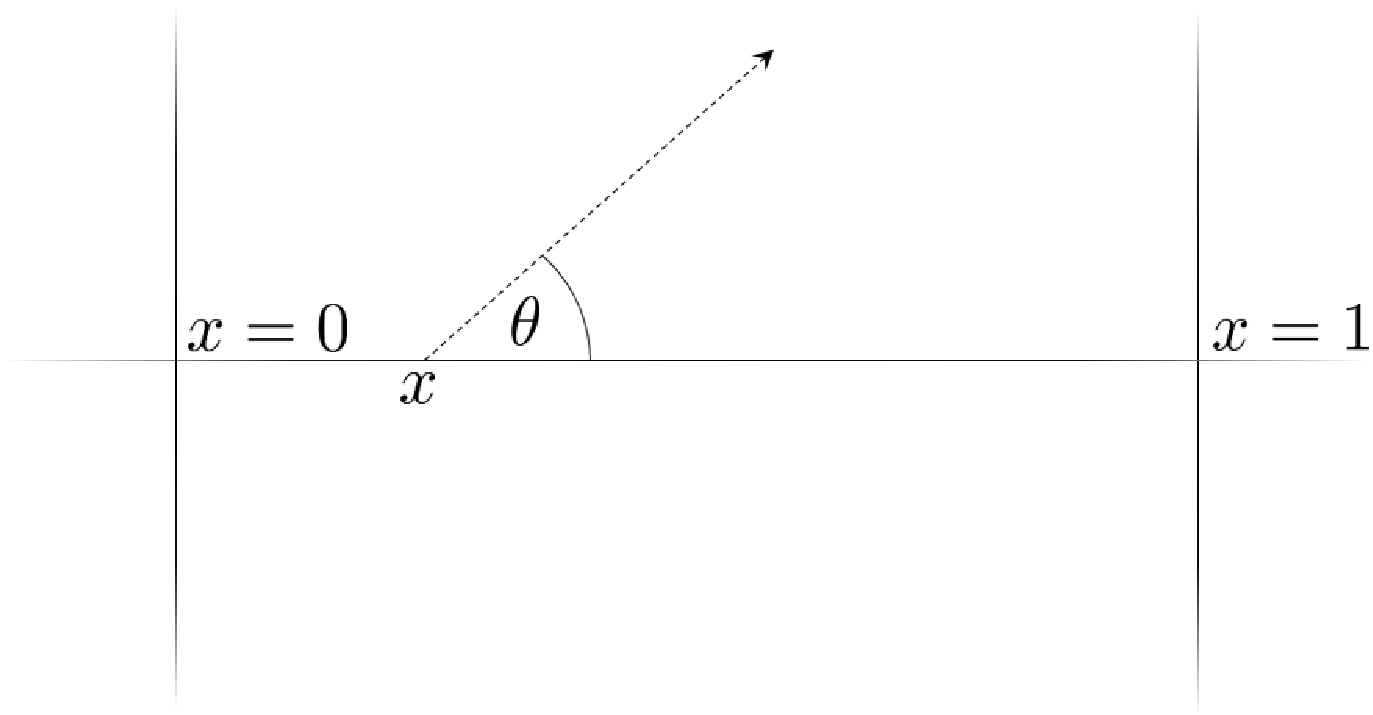
\includegraphics[width=0.5\linewidth]{figuras/geom.pdf}
  \caption{Geometría unidimensional: $\xi = \cos(\theta)$.}
 \label{fig:parallelgeom}
\end{figure}
La ecuación ETR independiente del tiempo, en una dimensión espacial 
modela el transporte en una geometría plana paralela descripta en la 
figura~\ref{fig:parallelgeom}. Por simplicidad, consideramos 
el caso isótropo, con condiciones de borde de Fresnel
\begin{equation}
\begin{split}
  &\xi \frac{\partial}{\partial x}\uxi+\mu_t(x)\uxi=   \frac{\mu_s(x)}{2} \int_{-1}^{1}\uxp d\xi' +q(x,\xi),\\
  &u(x=0,\xi)=\mathcal{R}(\xi)u(x=0,\xi_R) \; \forall \xi>0,\\
  &u(x=1,\xi)=\mathcal{R}(\xi)u(x=1,\xi_R) \; \forall \xi<0.
\end{split}
\label{eq:transp1d}
\end{equation}
donde $\xi=\cos(\theta)$,  $\mu_s(x)$ y $\mu_a(x)$ denotan 
los coeficientes de dispersión y absorción respectivamente, 
llamamos $\st(x)=\sa(x)+\mu_s(x)$ al coeficiente de transporte 
total, y $q(x,\xi)$ representa una fuente externa. Las condiciones de 
borde de Fresnel modelan la reflexión de las partículas en el borde, 
donde $\xi_R=-\xi$ representa el coseno de la dirección reflejada 
y $\mathcal{R}(\xi)$ es el coeficiente de Fresnel correspondiente~\cite{Born1999}.


Dado que el coeficiente $\xi$ que acompaña a la derivada de mayor 
orden en~\eqref{eq:transp1d} tiende a cero cuando $\theta \to \pi/2$, 
se espera que ocurra una capa límite que presente variaciones rápidas 
en la solución $u(x,\xi)$ para tales direcciones, y para valores 
de $x$ en regiones cercanas a los bordes en $x=0$ y $x=1$.
Como consecuencia surgirán gradientes que 
tienden a infinito para puntos $(x,\xi)$ cercanos a $(0,0)$ y $(1,0)$. 
Estas estructuras de capa límite, que son generadas por 
la imposición de las condiciones de borde en conjunto con la existencia 
de un parámetro $\xi$ infinitesimal que acompaña a la derivada de mayor 
orden del operador diferencial. En nuestro caso particular 
las condiciones de borde son impuestas en~~\eqref{eq:transp1d} para las direcciones 
entrantes (salientes), con $\xi>0$ ($\xi<0$) para puntos cercanos 
a $x=0$, (resp. $x=1$)---y es para dichas direcciones que 
se espera la aparición de la capa límite.

Siguiendo la referencia~\cite{Bender1999}, para caracterizar
la estructura de capa límite en \eg $x=0$, utilizamos una 
{\em solución interna} de la forma $U(X,\xi) = u(\xi X,\xi)$; 
la capa límite alrededor de $x=1$ puede ser tratada de manera 
análoga. La solución asintótica de primer orden $U_0(X,\xi)$ 
de $U(X,\xi)$ cuando $\xi\to 0^+$ satisface la ecuación 
a {\em coeficientes constantes} 
\begin{equation}
\begin{split}
\frac{\partial U_0(X,\xi)}{\partial X}& + \mu_t(0) U_0(X,\xi)=\frac{\mu_s(0)}{2} 
\int_{-1}^{1} U_0\left(\frac{\xi X}{\xi'},\xi'\right) d\xi' +q(0,\xi),\\
\end{split}
\label{eq:transp1d2}
\end{equation}
con condiciones de borde inducidas por~\eqref{eq:transp1d}. 
La ecuación~\eqref{eq:transp1d2} nos dice que la derivada 
$\frac{\partial U_0(X,\xi)}{\partial X}$ se encuentra 
acotada cuando $\xi\to 0^+$, y, por lo tanto, que la función 
$U_0(X,\xi)$ caracteriza la estructura de capa límite 
en la solución $u(x,\xi)$ mediante la relación 
\begin{equation}
  u(x,\xi)\sim u_0(x,\xi) = U_0(x/\xi,\xi) \; \text{sí}  \;  (x,\xi)\to (0^+,0^+).
\end{equation}
El argumento puede extenderse a problemas en dos y tres dimensiones, 
incluyendo el dominio temporal y dominios generales curvos. En tales casos, 
la capa límite presenta gradientes que no están acotados 
en la proximidad de los bordes en direcciones paralelas a estos 
(situación que a escalas apropiadas se corresponde con la geometría 
de la fig.~\ref{fig:parallelgeom} para $\theta \to \pi/2$). 

Utilizando el factor integrante, y definiendo
\begin{equation*}
I(x,\xi) = \int_0^{x} e^{\frac{ \mu_t(0) y}{\xi}}\left[\frac{\mu_s(0)}{2} \int_{-1}^1u_0(y,\xi')d\xi'+q(0,\xi)\right]dy,
\end{equation*}
se obtiene
\begin{equation}
 u_0(x,\xi) = \frac{e^{-\mu_t(0)x/\xi}}{\xi} \Big[\xi u(0,\xi)+I(x,\xi)\Big] ,
 \label{eq:intf}
\end{equation}
la cual exhibe de manera explícita el carácter exponencial 
de la capa límite. Los distintos términos de la solución asintótica 
para la capa límite poseen diferente interpretación física. Expandiendo 
la igualdad~\eqref{eq:intf} podemos escribir
\begin{equation}
\begin{aligned}
 u_0(x,\xi) =   e^{-\mu_t(0)x/\xi}\times u(0,\xi) + \frac{e^{-\mu_t(0)x/\xi}}{\xi} \times  \int_0^{x} e^{\frac{ \mu_t(0) y}{\xi}} \frac{\mu_s(0)}{2} \int_{-1}^1u_0(y,\xi')d\xi'dy&\\
 + \frac{e^{-\mu_t(0)x/\xi}}{\xi} \times \int_0^{x} e^{\frac{ \mu_t(0) y}{\xi}}  q(0,\xi) dy&,
 \label{eq:intfexpandida}
\end{aligned}
\end{equation}
donde el primer término representa el flujo entrante a través del borde en la dirección $\xi$ 
que no ha sufrido colisiones, el cual posee una atenuación exponencial 
debido a las interacciones de absorción y dispersión con el medio. El segundo término representa las contribuciones 
del medio debido a los procesos dispersivos, que sufren tanto una atenuación 
como un crecimiento exponencial, debido a la suma de contribuciones en el interior del medio. Finalmente, el último representa 
las contribuciones del medio debido a las fuentes $q$ en el interior de éste, 
las cuales también vienen dadas por contribuciones y atenuaciones en el interior del medio.

La estructura de capa límite puede visualizarse fácilmente 
considerando la solución exacta de la ecuación~\eqref{eq:transp1d} 
para el caso de coeficientes constantes sin dispersión ($\mu_s(x)=0$), 
de donde obtiene la solución analítica 
\begin{equation}
\begin{split}
u(x,\xi)=\begin{cases}
\displaystyle \frac{q}{\mu_a}\left[1-\frac{\eta(\xi)}{ e^{\mu_a x / \xi}}\right]&\forall\xi>0,\\[8pt]
%\displaystyle  \frac{q}{\mu_a}&\;\;\xi=0,\\
\displaystyle  \frac{q}{\mu_a}\left[1- \frac{\eta(\xi)}{e^{\mu_a (x-1) / \xi}} \right]&\forall\xi<0,
\end{cases}
\end{split}
\label{eq:transpnscatt}
\end{equation}
con
\begin{equation*}
\;\;\eta(\xi)=\frac{\mathcal{R}(|\xi|)-1}{\mathcal{R}(|\xi|)e^{-\mu_a/|\xi|}-1}.\qquad\qquad\qquad
\end{equation*}
Por simplicidad, consideramos condiciones de borde de vacío ($\mathcal{R}(\xi)=0$).
La solución se muestra en la figura~\ref{fig:ansol}, donde se observa claramente la estructura de capa 
límite cuando $(x,\xi) \to (0^+,0^+)$.
\begin{figure}[h!]
\centering
  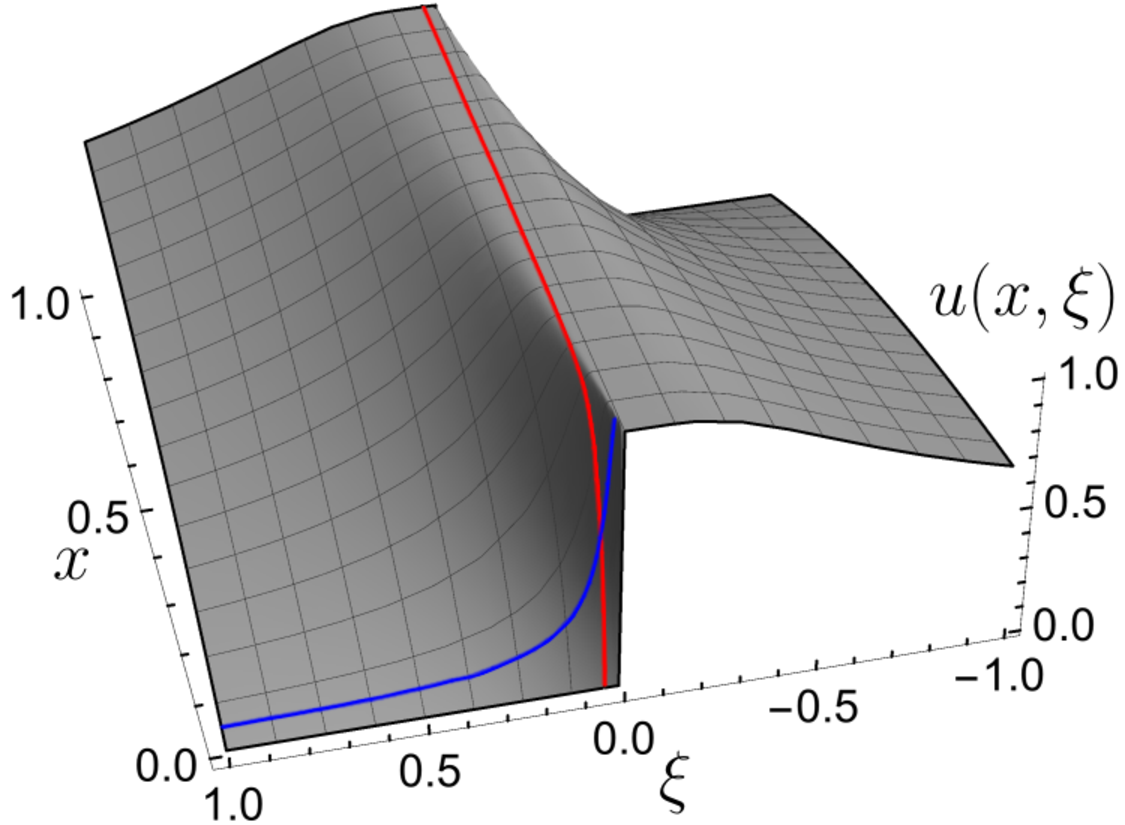
\includegraphics[width=0.5\linewidth]{figuras/Analytic_lay_3.pdf}
  \caption{Solución~\eqref{eq:transpnscatt} $\uxi$ de la ecuación.~\eqref{eq:transp1d} con
  $\mathcal{R}(\xi)=0$. Se observa la capa límite en las variables $x$ y $\xi$ 
  para $(x,\xi) \to (0^+,0^+)$ (enfatizadas en las curvas roja y azul).}
 \label{fig:ansol}
\end{figure}

Los dos métodos numéricos utilizados de manera predominante 
para resolver la ecuación de transporte son 
el método de armónicos esféricos,  
y el método de ordenadas discretas. Ambos fallan 
en la resolución de las estructuras de capa límite, 
lo cual puede apreciarse en resultados presentados 
en la literatura~\cite{Rocheleau2020,Wang2019,Harel2020,Anli2006,Chai1993}.

En vista de la expresión~\cite[p. 77]{Trefethen2008} 
para el término del error en la cuadratura de integración 
de Gauss--Legandre, el error para la cuadratura de $\ell$-puntos 
decrece como $32V/15\pi j (2\ell+1-j)^j$ siempre que la derivada 
$j \leq 2\ell$ esté acotada por la constante $V$. 
Introduciendo el cambio de variable  $\xi'=r^p$ en la integral 
de la ecuación~\eqref{eq:transp1d}, buscamos una cota $V$ 
para la derivada $j$--ésima del integrando. 
Utilizando la versión integrada de la ecuación~\eqref{eq:transp1d}, 
similar a~\eqref{eq:intf}, combinando dos términos exponenciales, 
y utilizando el hecho de que para un entero no negativo $k$ 
la integral $\int_0^\infty t^k e^{-t} dt$ es finita, 
encontramos qué (Apéndice~\ref{ap:demcv})
\begin{equation}
\begin{split}
\left | \frac{\partial^j }{\partial r^j}\left[ u(x,r^p) r^{p-1}\right]
\right|\leq W r^{p-j-1}\; \text{para}  \; (x,r) \to (0^+,0^+),
\end{split}
\label{eq:boundedderblayer}
\end{equation}
para alguna constante $W$; llamando $V = W r^{p-j-1}$  
se obtiene la cota deseada, la cual es {\em uniforme 
para todos los valores relevantes de $x$ y $r$ } (siempre que 
$p \ge j+1$). Los 
detalles de la demostración pueden encontrarse en el Apéndice~\ref{ap:demcv}.

Para el caso considerado, con $\mathcal{R}(\xi)=0$, 
dividiendo la integral en el punto de capa límite $\xi=0$ se tiene 
\begin{equation}
\int_{0}^{1} u(x,\xi) d\xi \sim \sum_{i=1}^{M/2} w_i u(x,\xi_i) \, .
\label{eq:MartensenKussmaul}
\end{equation}
Llamando $r_i$ y $w_i^{GL}$ a las abscisas y pesos de la 
cuadratura de Gauss--Legendre en el intervalo $[0,1]$, 
definimos $\xi_i=r_i^p$ y $w_i= p \times r_i^{p-1} \times w_i^{GL}/2$. 
Las abscisas y los pesos correspondientes a los valores negativos 
de $\xi$ se obtienen por simetría. 
\begin{figure}[h!]
\centering
  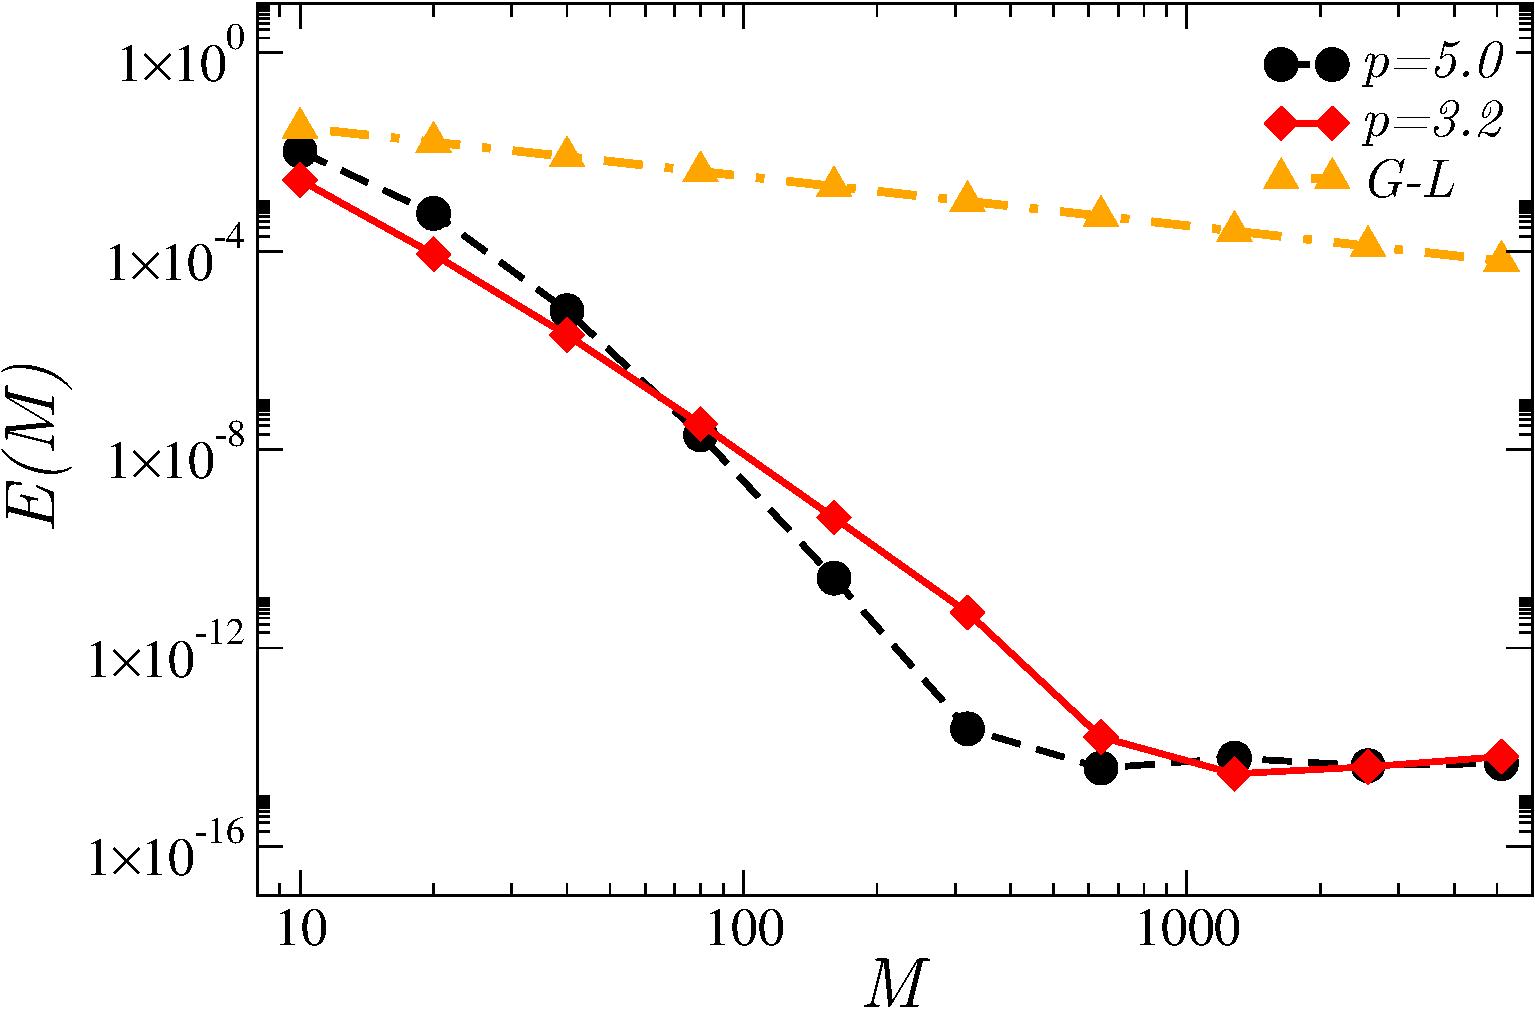
\includegraphics[width=0.5\linewidth]{figuras/quads.pdf}
  \caption{Error de la integral numérica respecto a la 
  analítica $E(M)=\text{max}_x |\sum_{i=1}^M w_i u(x,\xi_i)-I^{\text{an}}(x)|$
  obtenida para la solución~\eqref{eq:transpnscatt} con $\mathcal{R}(\xi)=0$. 
  Los errores fueron obtenidos para la cuadratura~\eqref{eq:MartensenKussmaul} 
  para $p=5$ y $p=3.2$. G--L: 
  Error dado por la cuadratura de Gauss--Legendre sin el cambio de variable propuesto.}
 \label{fig:intconvs}
\end{figure}
Se encontró el valor $p=3.2$ como óptimo, el cual 
provee una convergencia excelente para la integral 
de dispersión en la variable $\xi$, y a su vez limita la rapidez 
de las variaciones de la capa límite en la variable espacial $x$. 

Para resolver la capa límite en $x$, utilizamos 
el cambio de variable logarítmico $v=\log(\frac{x}{1-x})$, 
que origina una grilla con puntos extremadamente cercanos al borde. 
Dado que las cotas halladas~\eqref{eq:boundedderblayer} para las derivadas del 
integrando con respecto a la nueva variable $r$ son {\em uniformes para todo $x$},  
el procedimiento no deteriora la convergencia de la 
cuadratura de la integral colisional.  Por lo tanto 
se logra un alto orden de convergencia en ambas variables $\xi$ y $x$

Resolvemos la ecuación de transporte que resulta en el nuevo dominio computacional
$[v_{\text{min}},v_{\text{max}}]$, con 
$[x'_{\text{min}},x'_{\text{max}}]=[\frac{e^{v_{\text{min}}}}{e^{v_{\text{min}}}+1},
\frac{e^{v_{\text{max}}}}{e^{v_{\text{max}}}+1}]$, 
y condiciones de bordes en $x'_{\text{min}}$ y $x'_{\text{max}}$ 
obtenidas a partir de la solución asintótica~\eqref{eq:intf}. Utilizando las nuevas variables, 
el problema de transporte dependiente del tiempo resulta 
\begin{wrapfigure}{r}{0.45\textwidth}
  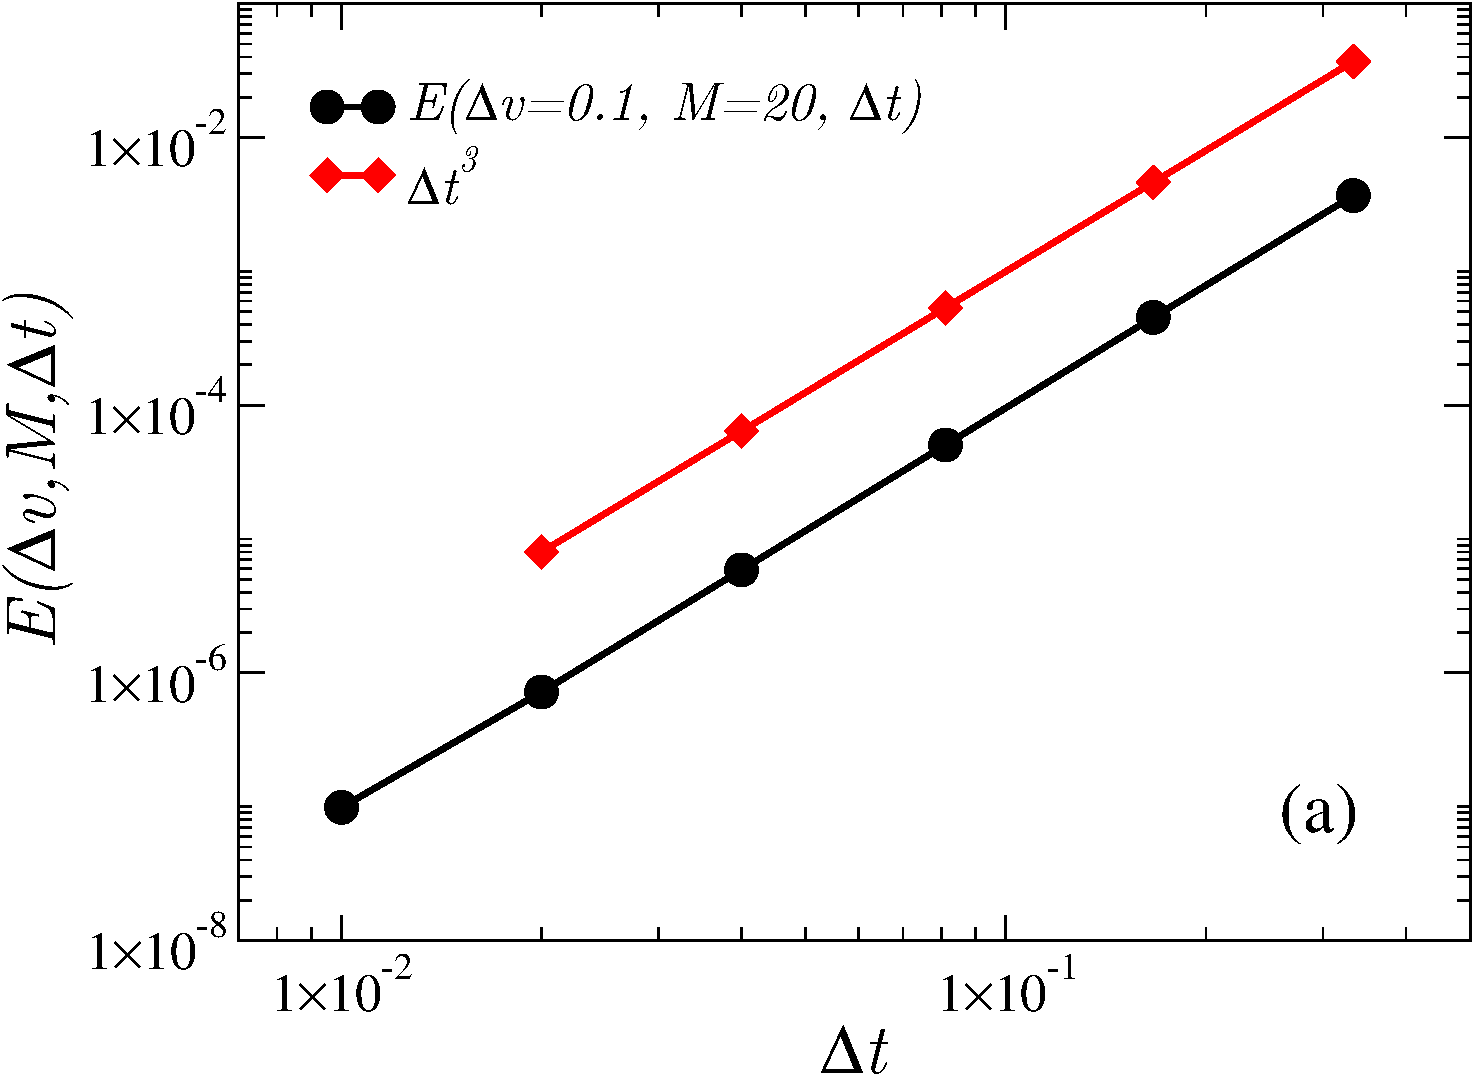
\includegraphics[width=0.45\textwidth]{figuras/errdt.pdf}\\
  \vspace{2mm}
  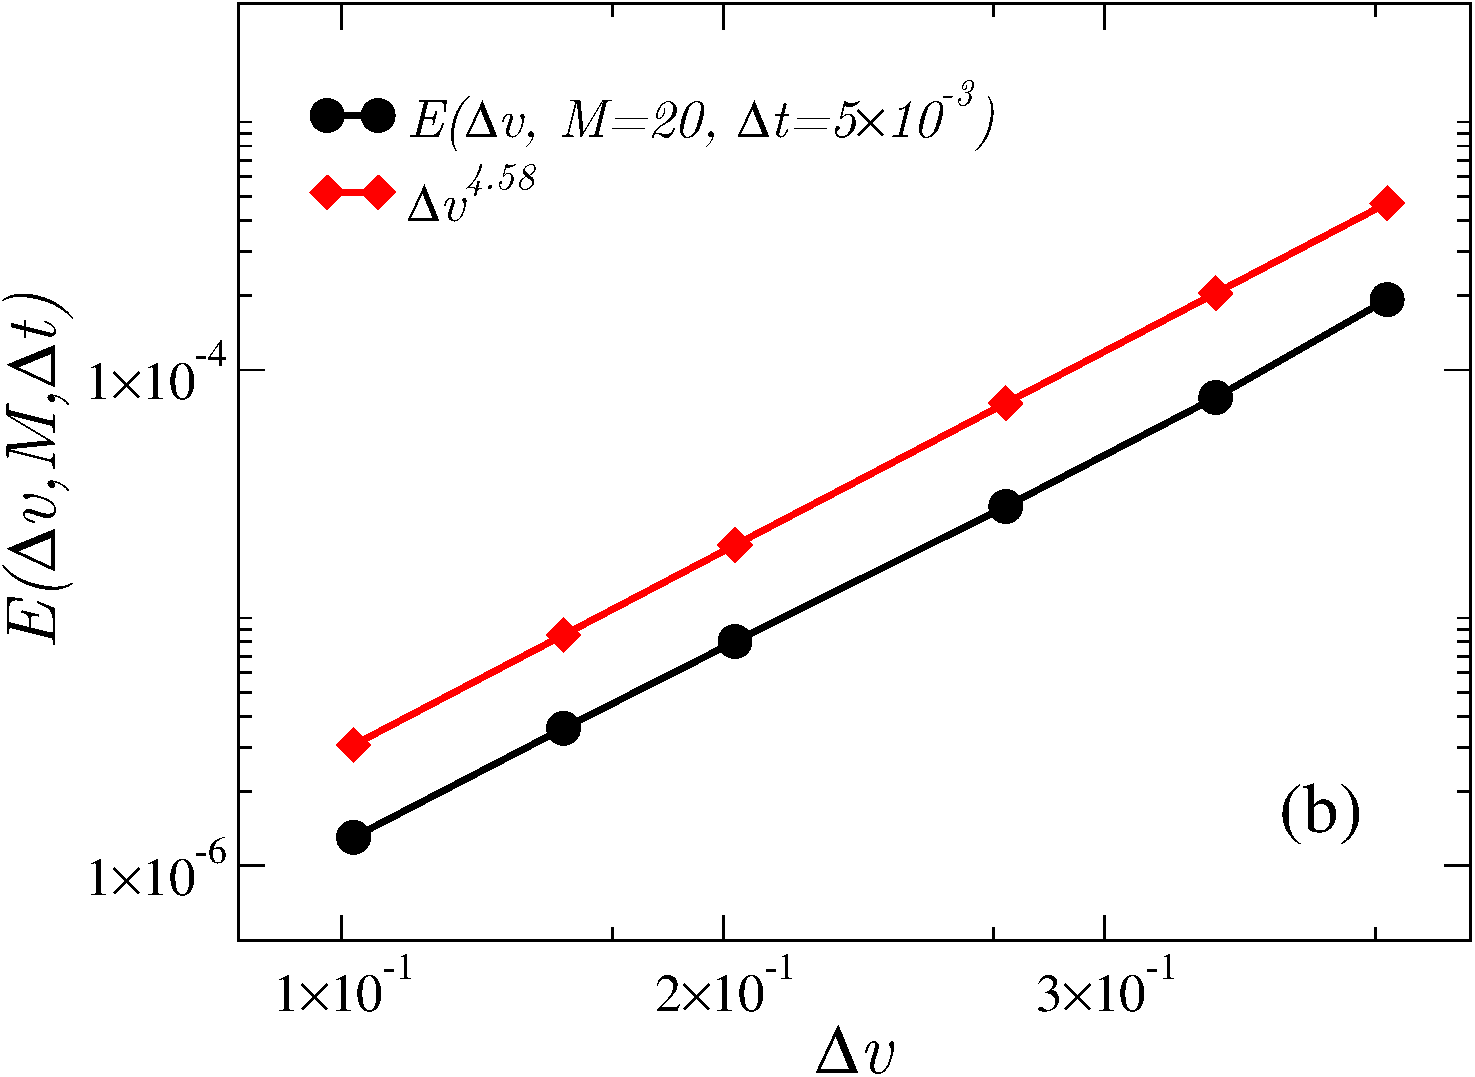
\includegraphics[width=0.45\textwidth]{figuras/errdx.pdf}\\
  \vspace{2mm}
  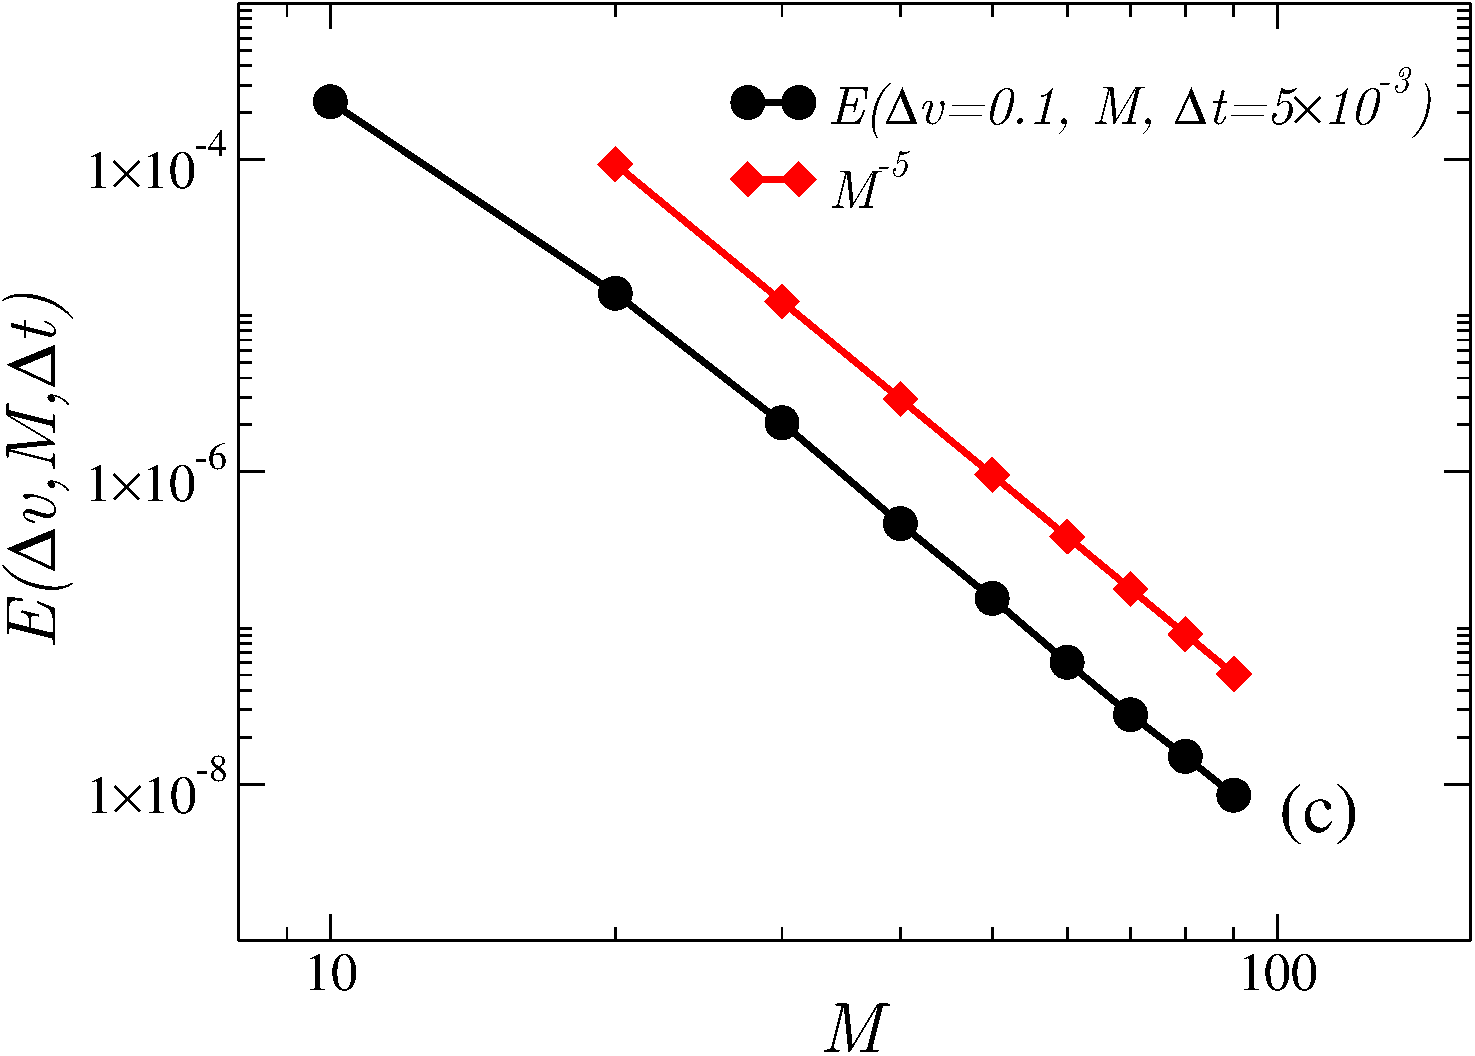
\includegraphics[width=0.45\textwidth]{figuras/xiconv.pdf}
  \caption{Círculos: error obtenido en diferentes grillas numéricas para el algoritmo 
  propuesto. Diamantes: orden de convergencia.}
 \label{fig:conv}
\end{wrapfigure}
\begin{equation}
\begin{split}
&\frac{\partial}{\partial t}\uvi+\xi(2+2\cosh(v)) \frac{\partial}{\partial v}\uvi\\
&+\st\uvi=\sct \int_{-1}^{1} \uvp d\xi'+q, \\
&u(v,\xi,t_{\text{min}})=0,\\
&u(v_{\text{min}},\xi,t)=u_{0}(x'_{\text{min}},\xi,t) \; \forall \xi>0,\\
&u(v_{\text{max}},\xi,t)=u_{0}(x'_{\text{max}},\xi,t) \; \forall \xi<0.
\end{split}
\label{eq:transptd}
\end{equation}
Con el fin de evitar las
limitaciones impuestas por la condición de CFL, utilizamos un 
esquema implícito BDF ({\em backward differentiation formula}) de evolución temporal de tercer orden. 
Para evitar el alto costo en la inversión de matrices grandes a 
cada paso temporal, el término 
colisional se obtiene por extrapolación polinomial. La versión discreta con propagación temporal 
implícita de la Ecuación~\eqref{eq:transptd} resulta
\begin{equation*}
\begin{aligned}
 \left[ \id \right. & \left.+ \beta\Delta t\xi_j (2+2\cosh(v)) \ide + \beta\Delta t \mu_t \id \right]  
 u^{n+1}_j  = \\
&\sum_{k=0}^{s-1}\alpha_k u_j^{n-k} + \beta\Delta t \sct
 \sum_{i=1}^{M} w_i \tilde{u}_i^{n+1} + \beta\Delta t q^{n+1},
\end{aligned}
\label{eq:transptd1disc}
\end{equation*}
donde $u^{n+1}_j=u(v,\xi_j,t^{n+1})$, $t^{n+1}=n\Delta t$, siendo $\alpha_k$ y $\beta$ 
los coeficientes BDF, con $s=3$. El término extrapolado 
a tercer orden viene dado por $\tilde{u}_j^{n+1}=\sum_{\kappa=0}^{2}(-1)^\kappa {3 \choose \kappa+1} u_j^{n-\kappa}$. Nuevamente, 
$\id$ es el operador identidad, mientras qué $\ide$ representa al operador 
de diferenciación espectral obtenido mediante el método de continuación de Fourier. 

La Fig.~\eqref{fig:conv} muestra las excelentes propiedades de convergencia 
obtenidas mediante el algoritmo propuesto para $\mu_s=\mu_a=q=1$. Dado 
que no se conoce una solución analítica para este problema, calculamos 
el error comparando las soluciones en diferentes grillas, tomando 
como referencia a la más fina de ellas. El alto orden 
de convergencia obtenido sugiere que los cambios de variables 
propuestos en $x$ y $\xi$ permiten 
resolver las capas límite en ambas variables. 
Se definió el error para las Figuras~\eqref{fig:conv} (a) y (b) según
  $E(\Delta v, M,\Delta t)=\text{max}_{x,\xi}
    |u(x,\xi)-u^{\text{c}}(x,\xi)|$, donde $u^{\text{c}}(x,\xi)$ 
    es la solución convergida, obtenida en la grilla mas fina. 
Debido a que las diferentes 
    grillas direccionales poseen abscisas que no coinciden 
    entre sí,  
    el error calculado en la Fig. (c) utiliza el flujo escalar, con  
$E(\Delta v, M,\Delta t)=\text{max}_x |\sum_{i=1}^M w_i u(x,\xi_i)-\phi^{\text{c}}(x)|$.

A continuación, emplearemos el algoritmo propuesto para 
explorar y demostrar el carácter de las estructuras de capa límite. 
Por simplicidad, en el resto de este capítulo nos restringiremos 
al caso de la ETR independiente del tiempo. 
Como se describió anteriormente 
en la Sección~\ref{sec:resexp}, las soluciones se obtienen 
evaluando las evoluciones temporales a tiempos asintóticos.
Estas se muestran en las Figuras~\ref{fig:blayers1} 
a~\ref{fig:DDlayer}.
\begin{figure}[h!]
\centering
  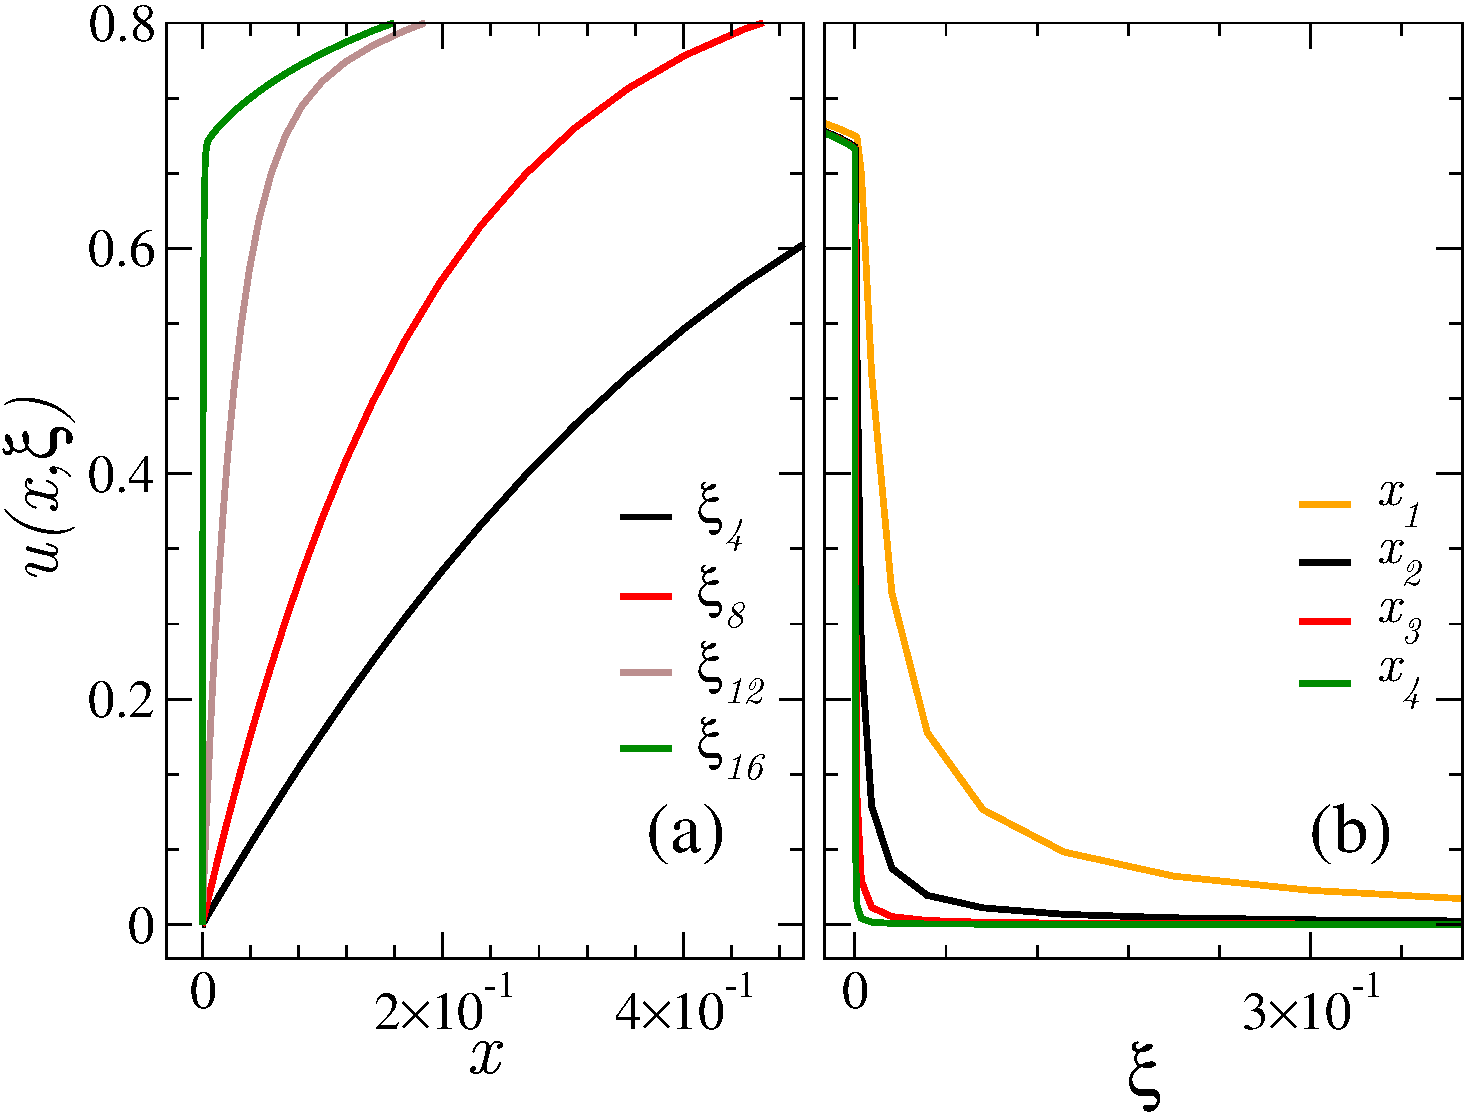
\includegraphics[width=0.5\linewidth]{figuras/xilay.pdf}
  \caption{Capas límite obtenidas como solución 
  de la ecuación~\eqref{eq:transptd} para un entorno de $x=0$ y $\xi=0$, 
  con $\mu_a=\mu_s=q=1$ para distintos valores de $\xi$ y de $x$, 
  con $\xi_i>\xi_{i+1}>0$ y $x_i>x_{i+1}$.}
 \label{fig:blayers1}
\end{figure}
La Fig.~\ref{fig:blayers1} muestra las estructuras de capa límite en las 
variables $x$ y $\xi$ con $\mu_s=\mu_a=q=1$ (con parámetros numéricos $N=250$, $M=40$, 
y $-v_{\text{min}}=v_{\text{max}}=25$). Como puede observarse, 
los valores más chicos de $\xi$ 
originan capas límite que se comprimen en regiones espaciales más 
pequeñas, tal como sugiere el análisis realizado. 
La Fig.~\ref{fig:blayers} muestra la existencia de 
de capas límite incluso para medios altamente difusivos, con 
$\mu_a=q=1$ fijo. En esta figura, 
$\xi=\xi_{\text{min}}\simeq 10^{-6}$, para los parámetros 
$N=200$, $M=20$ y $-v_{\text{min}}=v_{\text{max}}=20$. 
En general, en problemas difusivos 
(donde $\mu_s>>\mu_a$ y $\mu_s>>q$ y $\mu_s>>|x_{\text{max}}-x_{\text{min}}|$) 
las funciones tienden a ser mas regulares en la variable $\xi$~\cite{Larsen1987}. 
Siendo la dispersión el fenómeno dominante, 
la solución resulta fuertemente ``promediada'' entre las direcciones.  
Sin embargo, tienden a tener pendientes más abruptas 
a medida que aumenta el coeficiente de dispersión. Cuando la dispersión es grande, 
se verfica numéricamente que 
 $u(x,\xi)$ es prácticamente independiente de la dirección, excepto en la región 
de capa límite.
\begin{figure}[h!]
\centering
  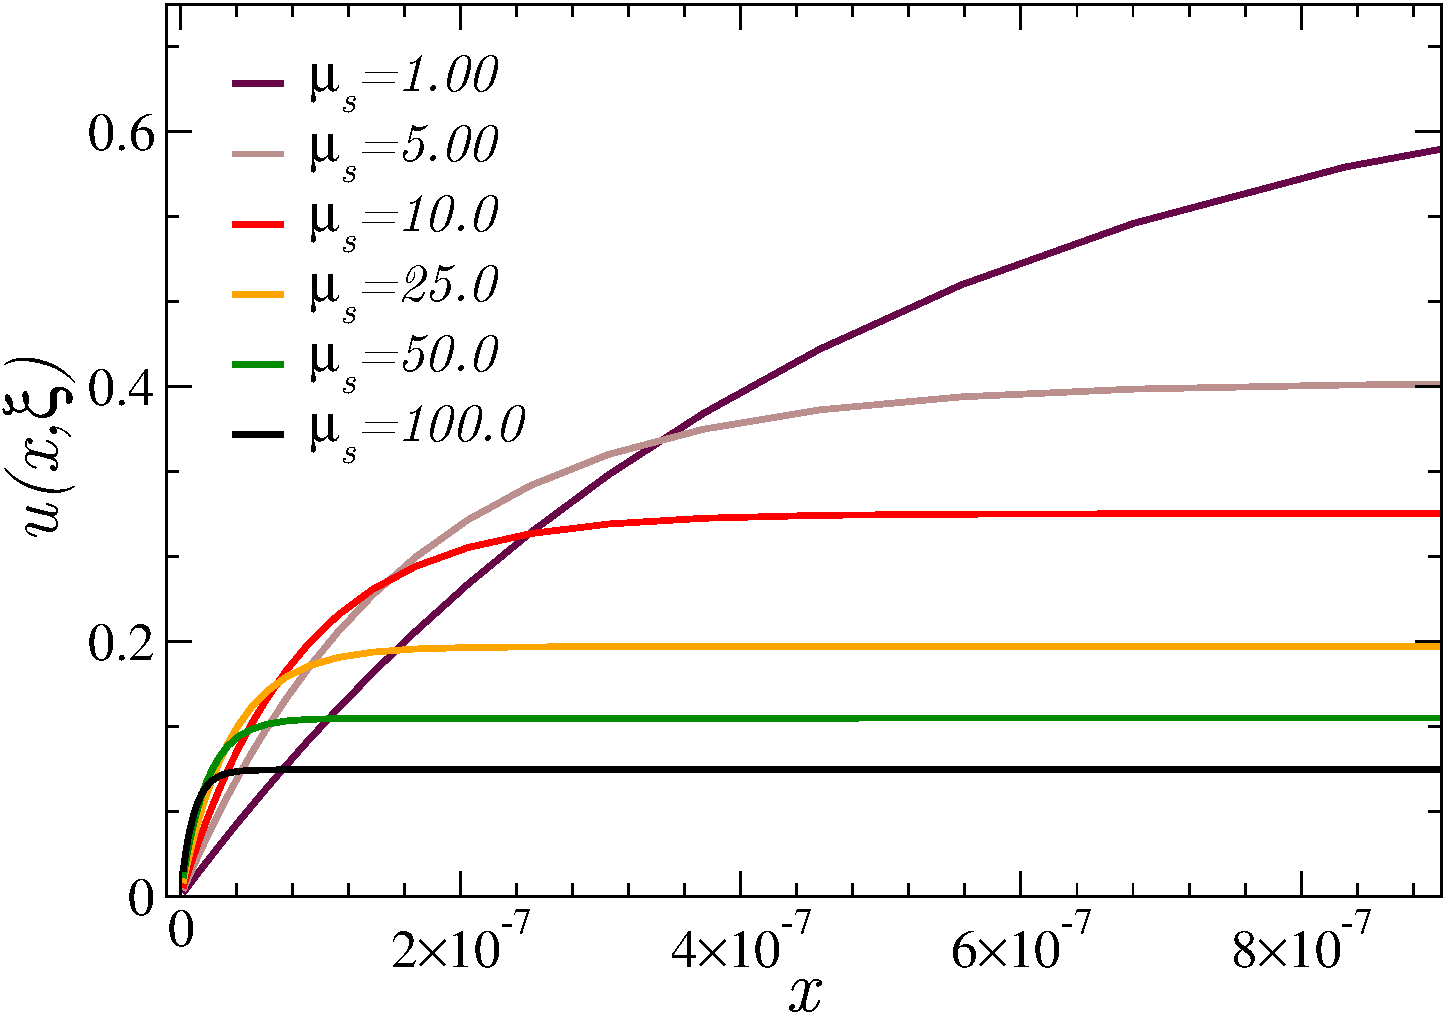
\includegraphics[width=0.5\linewidth]{figuras/blayers.pdf}
  \caption{Capas límite obtenidas resolviendo la ecuación~\eqref{eq:transptd}, 
  con $\mu_a=q=1$ para distintos valores de $\mu_s$. 
  Se muestran las soluciones para la dirección $\xi=\xi_{\text{min}} \simeq 10^{-6}$. 
  Notar las pendientes elevadas que existen para $x\to 0^+$.}
 \label{fig:blayers}
\end{figure}
Se ha reportado en la literatura la existencia 
de oscilaciones no físicas 
asociadas a problemas numéricos. 
Estas surgen principalmente al emplear el esquema de 
diferencias finitas de Diamante (DD)~\cite{Larsen1987,Petrovic1996,Bal2001}.
En las referencias~\cite{Larsen1987,Petrovic1996} se atribuye 
este problema numérico a las condiciones de borde anisótropas, capas límite no difusivas y/o 
a un alto coeficiente de absorción. Por el contrario, 
en nuestro trabajo demostramos que esta interpretación es errónea. 
Las capas límite surgen aún con condiciones de borde isótropas, 
y para cualquier valor 
de los coeficientes de absorción y dispersión. En particular, 
nuestra contribución demuestra en forma explícita la existencia 
de capas límite exponenciales, originadas al imponer cualquier 
condicion de borde para valores de  $\xi$ 
pequeños, lo cual no fue considerado en ninguno de los trabajos anteriores.

Por ejemplo, la referencia~\cite{Larsen1987} trata un problema 
difusivo de transporte (el Problema~1 en dicha referencia). 
Este es el mismo que plantea la Ecuación~\eqref{eq:transp1d} con $\mu_s=\mu_t=1000$,
 $q=0.1$ y $\mathcal{R}(\xi)=0$. Este es un caso  
 difusivo, con condiciones de borde isótropas, 
 sobre el que dicha referencia afirma~\cite[pp. 317]{Larsen1987} 
 ``\ldots dado que el término de orden dominante en la expansión asintótica 
 de la ecuación de transporte analítica es isótropo, 
 este término no posee una capa límite para este problema''. 
 En contraste, la Figura~\ref{fig:DDlayer} muestra que 
 las capas límite persisten en este problema, y 
 no fueron detectadas debido a que la grilla numérica utilizada 
 no era lo suficientemente densa como para resolverlas. 
 La solución obtenida por el método FC--DOM implícito,  
 con el cambio de variable propuesto, se obtuvo 
 con $M=40$ direcciones discretas y $N=400$ puntos 
 en la variable espacial. En comparación, en la implementación del esquema DD 
 se utilizaron $N=10000$ puntos. Aún teniendo en cuenta 
 el alto costo computacional que requiere este esquema, no logra 
 evitar las oscilaciones espurias.
\begin{figure}[h!]
\centering
  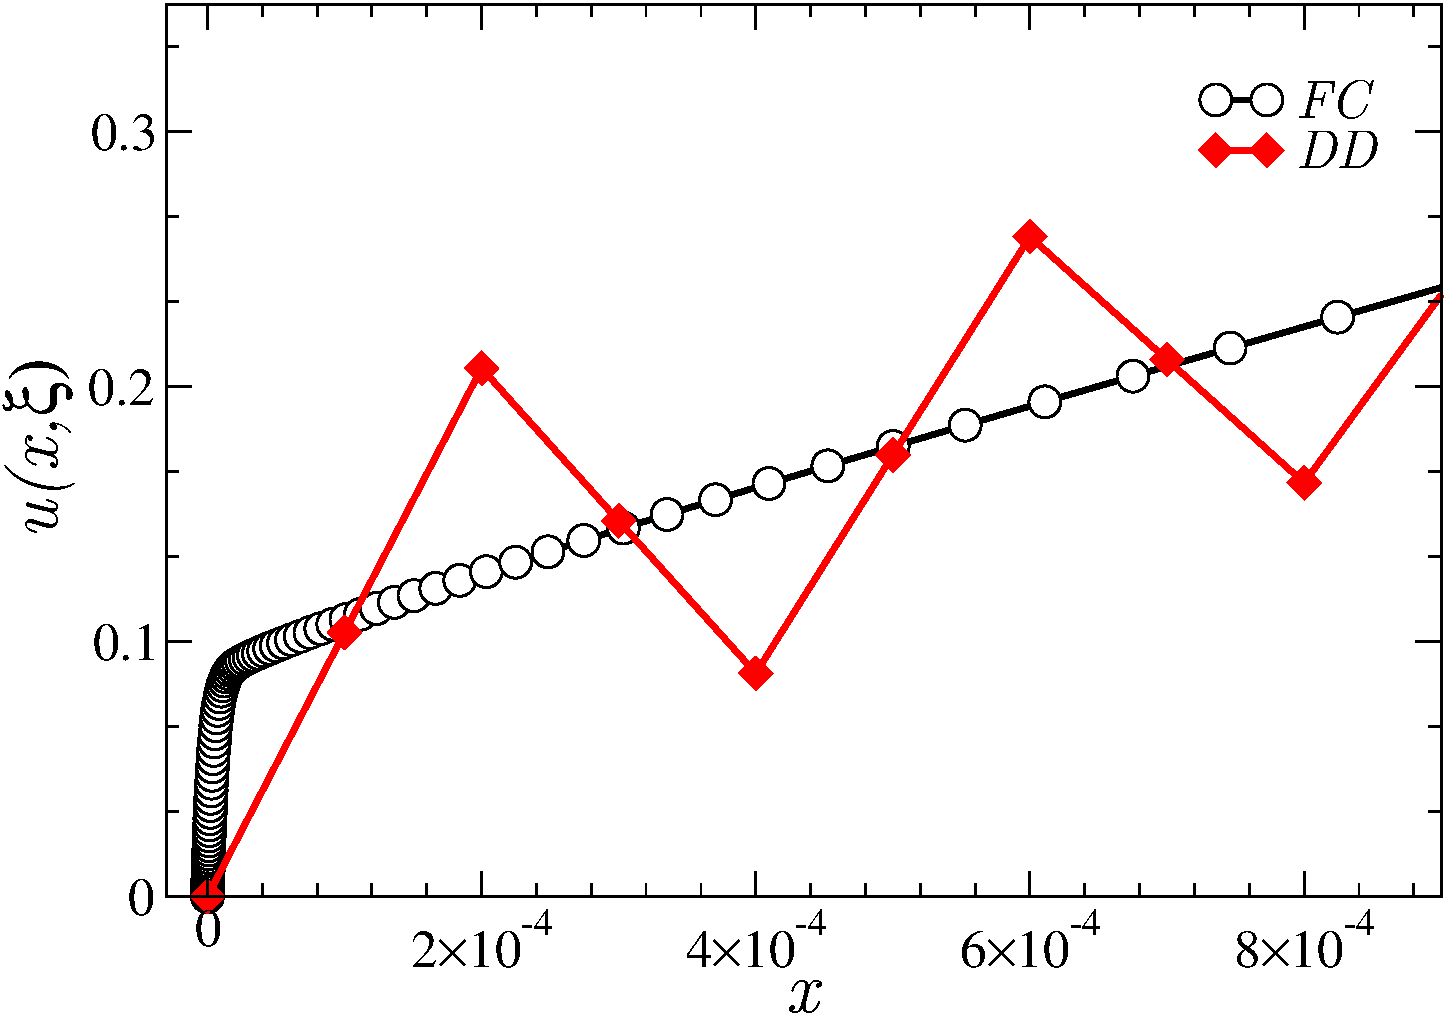
\includegraphics[width=0.5\linewidth]{figuras/layerlar.pdf}
  \caption{Solución $u(x,\xi_{15})$ de la ec.~\eqref{eq:transp1d} 
  con $\mu_t=\mu_s=1000$, $q=0.1$ y $\xi_{\text{15}} \simeq 10^{-3}$
  donde pueden apreciarse las oscilaciones espurias originadas 
  por el esquema DD. Se utilizaron $N=10000$ puntos espaciales para el método DD y 
  tan sólo $N=400$ para el FC.}
 \label{fig:DDlayer}
\end{figure}

En la Figura~\ref{fig:DDlayer2} se muestran las soluciones obtenidas por ambos esquemas 
en regiones lejanas a la capa límite, para distintas grillas espaciales. 
Puede apreciarse que si bien las oscilaciones que emergen del método DD lo hacen 
en cercanías del origen, 
se propagan hacia todo el dominio espacial.
\begin{figure}[h!]
\centering
  \includegraphics[width=0.5\linewidth]{figuras/conv_2.eps}
  \caption{Solución $u(x,\xi_{15})$ de la Ec.~\eqref{eq:transp1d}, 
  (cf. Fig.~\ref{fig:DDlayer}), para distintas grillas espaciales, 
  lejos de la región de capa límite. 
  Como se observa, las oscilaciones originadas en 
  las cercanías del borde por el esquema DD se extienden a todo el dominio espacial.}
 \label{fig:DDlayer2}
\end{figure}

Físicamente, los valores pequeños de $\xi$ para las direcciones 
entrantes en puntos espaciales $x$ cerca del borde (cf. fig.~\ref{fig:parallelgeom}) 
estan asociados a caminos geométricos largos, lo que da origen 
a las transiciones abruptas de capa límite observadas.
Esta estructura de capa límite, que no fue previamente reportada 
en la literatura, constituye un fenómeno físico que no fue correctamente 
descripto, ni caracterizado por varias décadas, y que como se demostró 
en la fig.~\ref{fig:DDlayer} y a lo largo de esta sección, 
posee importantes implicancias en la física y en las simulaciones 
numéricas de los fenómenos de transporte.

Cabe destacar que las estructuras de capa límite 
existen durante todos los tiempos de la evolución temporal. 
En particular, tanto el análisis asintótico de la capa límite que 
derivó en la ecuación~\eqref{eq:intf}, 
así como las pruebas numéricas, sugieren que existirá una capa límite 
siempre qué en un entorno del borde existan fuentes, haya dispersión, 
o condiciones de contorno no nulas. La teoría desarrollada predice 
una capa límite que se desarrollará con gradientes abruptos en regiones 
espaciales $x'$ de orden $x'\sim \ord(\xi/\mu_t(0))$, y en regiones direccionales $\xi'$  
de orden $\xi'\sim \ord(\mu_t(0) x)$. Si las grillas numéricas empleadas no resuelven 
correctamente estas regiones, las soluciones obtenidas para problemas 
que reflejan situaciones realistas para aplicaciones en tomografía óptica 
(y otras disciplinas donde se requiere la solución a la ecuación ETR con 
condiciones de contorno arbitrarias) gozarán de un orden de convergencia 
limitado por la existencia de derivadas no acotadas en el integrando 
colisional, y por la existencia de soluciones subyacentes que en el dominio 
espacial discretizado también lucirán como discontinuas debido a la falta de resolución 
en la grilla numérica, 
con consecuencias e implicaciones similares a las observadas 
en esta sección para la integral colisional en la fig.~\ref{fig:intconvs} 
para la aproximación 
numérica del operador diferencial en la ecuación de transporte. 

Si bien el desarrollo de algoritmos capaces de resolver las capas límite 
en más dimensiones espaciales es un tema de investigación vigente que escapa 
al alcance de esta tesis, los resultados obtenidos en el marco de la misma 
establecen los cimientos para la elaboración de nuevos métodos numéricos 
capaces de hacerlo, de relevancia e impacto en varias disciplinas tecnológicas 
y científicas. 

\pagestyle{empty}



\newpage
\chapter{El problema inverso}%
\lhead{\thepage}
\rhead{\textit{El problema inverso}} \\
\vspace{0.01\textheight}
\label{sec:inverso}
%\pagebreak

En las secciones previas abordamos el problema directo de transporte 
de radiación en la materia mediante la ETR. En síntesis, el problema 
directo consta de, dados los parámetros ópticos $a(\x)$, $b(\x)$, la función  
de fase $\eta(\hth\cdot \hth')$, la velocidad de la luz en el medio participante 
$c$, las fuentes internas $s$ y las condiciones iniciales y de contorno, 
encontrar la solución $\ut$ a la ecuación~\eqref{eq:RTE}.

Para el problema inverso en tomografía óptica, alguno de los parámetros 
ópticos es desconocido, 
o conocido sólo parcialmente, y se dispone de mediciones experimentales 
de detectores colocados en el contorno del dominio que se quiere analizar. 
A partir de las mediciones experimentales de estos detectores, 
el objetivo es la reconstrucción de uno o más de los parámetros ópticos. 
En el caso de tomografía por fluorescencia y tomografía de bioluminiscencia, lo que se intenta reconstruir 
son las fuentes $s$ en la ec.~\eqref{eq:RTE}~\cite{Klose2005,Klose2009,Ren2010}, 
que vienen relacionadas a los coeficientes de absorción de los 
cromoforos y fluoroforos. 

En el contexto de esta tesis, nos limitaremos a la reconstrucción del 
coeficiente de absorción, $a(\x)$. La reconstrucción de dicho coeficiente 
encuentra aplicaciones en tomografía de fluorescencia, y en tomografía óptica. 
La reconstrucción de las propiedades de absorción en tomografía óptica 
 permite la identificación de tumores~\cite{Zhu2005,Zhu2010,Fujii2016b}, 
la obtención de imagenes funcionales del cerebro humano~\cite{Boas2001,bluestone2001,Arridge1999}, 
y la caracterización de diferentes constituyentes del tejido 
humano para la obtención de imágenes en medicina. En 
este trabajo nos enfocamos en la reconstrucción del coeficiente 
de absorción, pero los algorítmos y las estrategias propuestas 
pueden ser fácilmente generalizadas para la reconstrución 
de otros parámetros. 

Generalmente, para aplicaciones 
en diágnostico y monitoreo en el tratamiento de tumores, 
se asume cierta información previa 
para el coeficiente de dispersión, 
$b(\x)$, obtenida por técnicas de obtención 
de imagenes de alta resolución~\cite{Althobaiti2017,Guven2003} \eg Resonancia Magnética. 
Este conocimiento previo obtenido por otras técnicas, también brinda 
información límitada en el parámetro óptico de absorción $a(\x)$, 
como pueden ser los coeficientes de absorción para ciertos tejidos óseos, 
o el aire en regiones como la traquea del cuello humano, como también 
se conocen cotas superiores e inferiores para dicho parámetro, 
lo que permite restringir el espacio de funciones donde se busca minimizar 
la función objetivo. El uso de técnicas de alta resolución, como la Resonancia 
Magnética, posee ciertas límitaciones, como el alto costo, la baja disponibilidad 
de este tipo de aparatos 
(lo que impone una dificultad a la hora de seguir la evolución de un tratamiento 
asistido por diagnóstico de imágenes), y adicionalmente los dispositivos 
utilizados en tomografía óptica son portables, lo que permite tenerlos disponibles 
para su uso en diversas situaciones. En la figura~\ref{fig:esquemainv} esquematizamos los problemas directos e inverso, tal como son 
tratados en esta tésis. 


\begin{figure}[h!]
\centering
  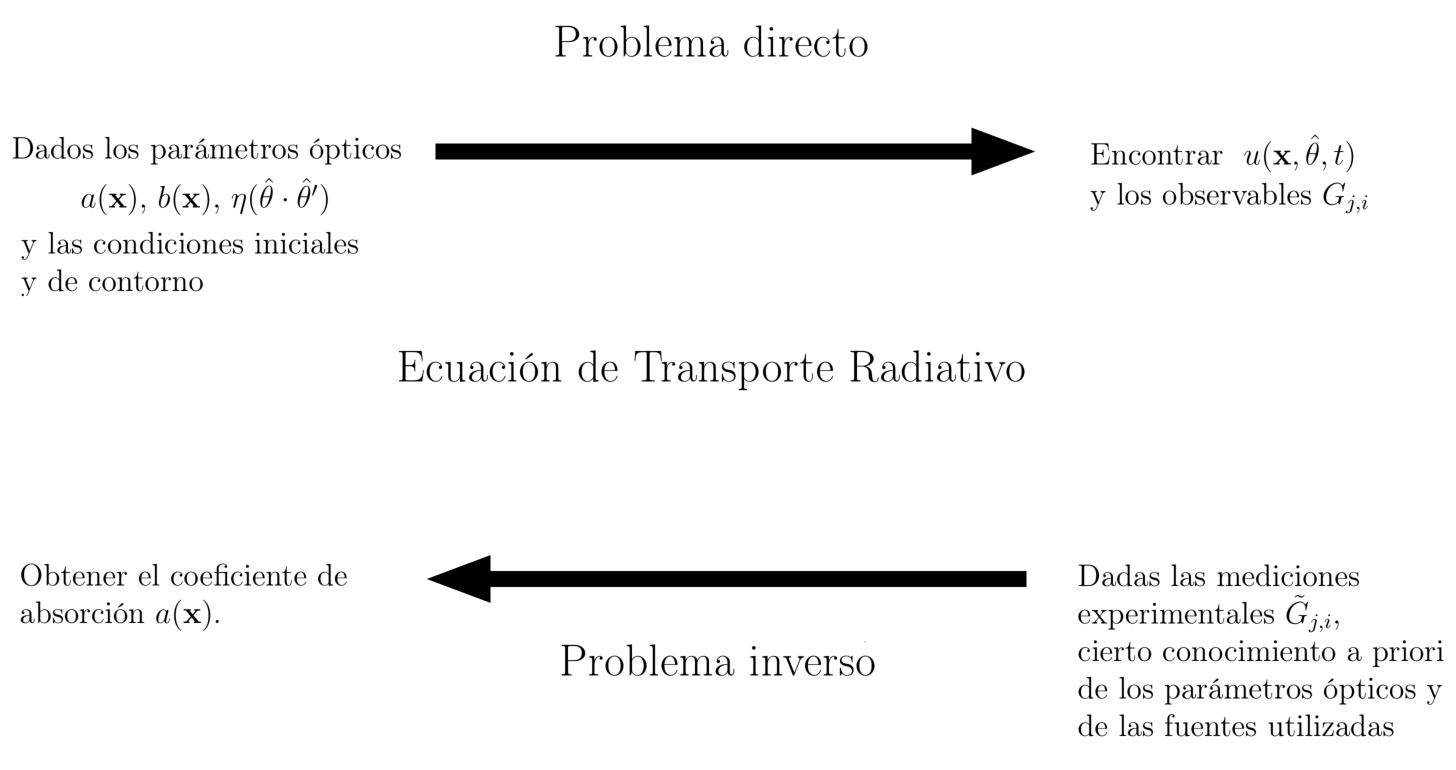
\includegraphics[width=\linewidth]{figuras/inv.pdf}\\
  \caption{
Grafico esquematico de los problemas directo e inverso, tal como son considerados 
en esta tésis.}
 \label{fig:esquemainv}
\end{figure}
Para la resolución del problema inverso, utilizamos el esquema \textit{MOBIR}, 
presentado en la sección siguiente. 

\section{El esquma \textit{MOBIR}}

\begin{wrapfigure}{l}{0.48\textwidth}
  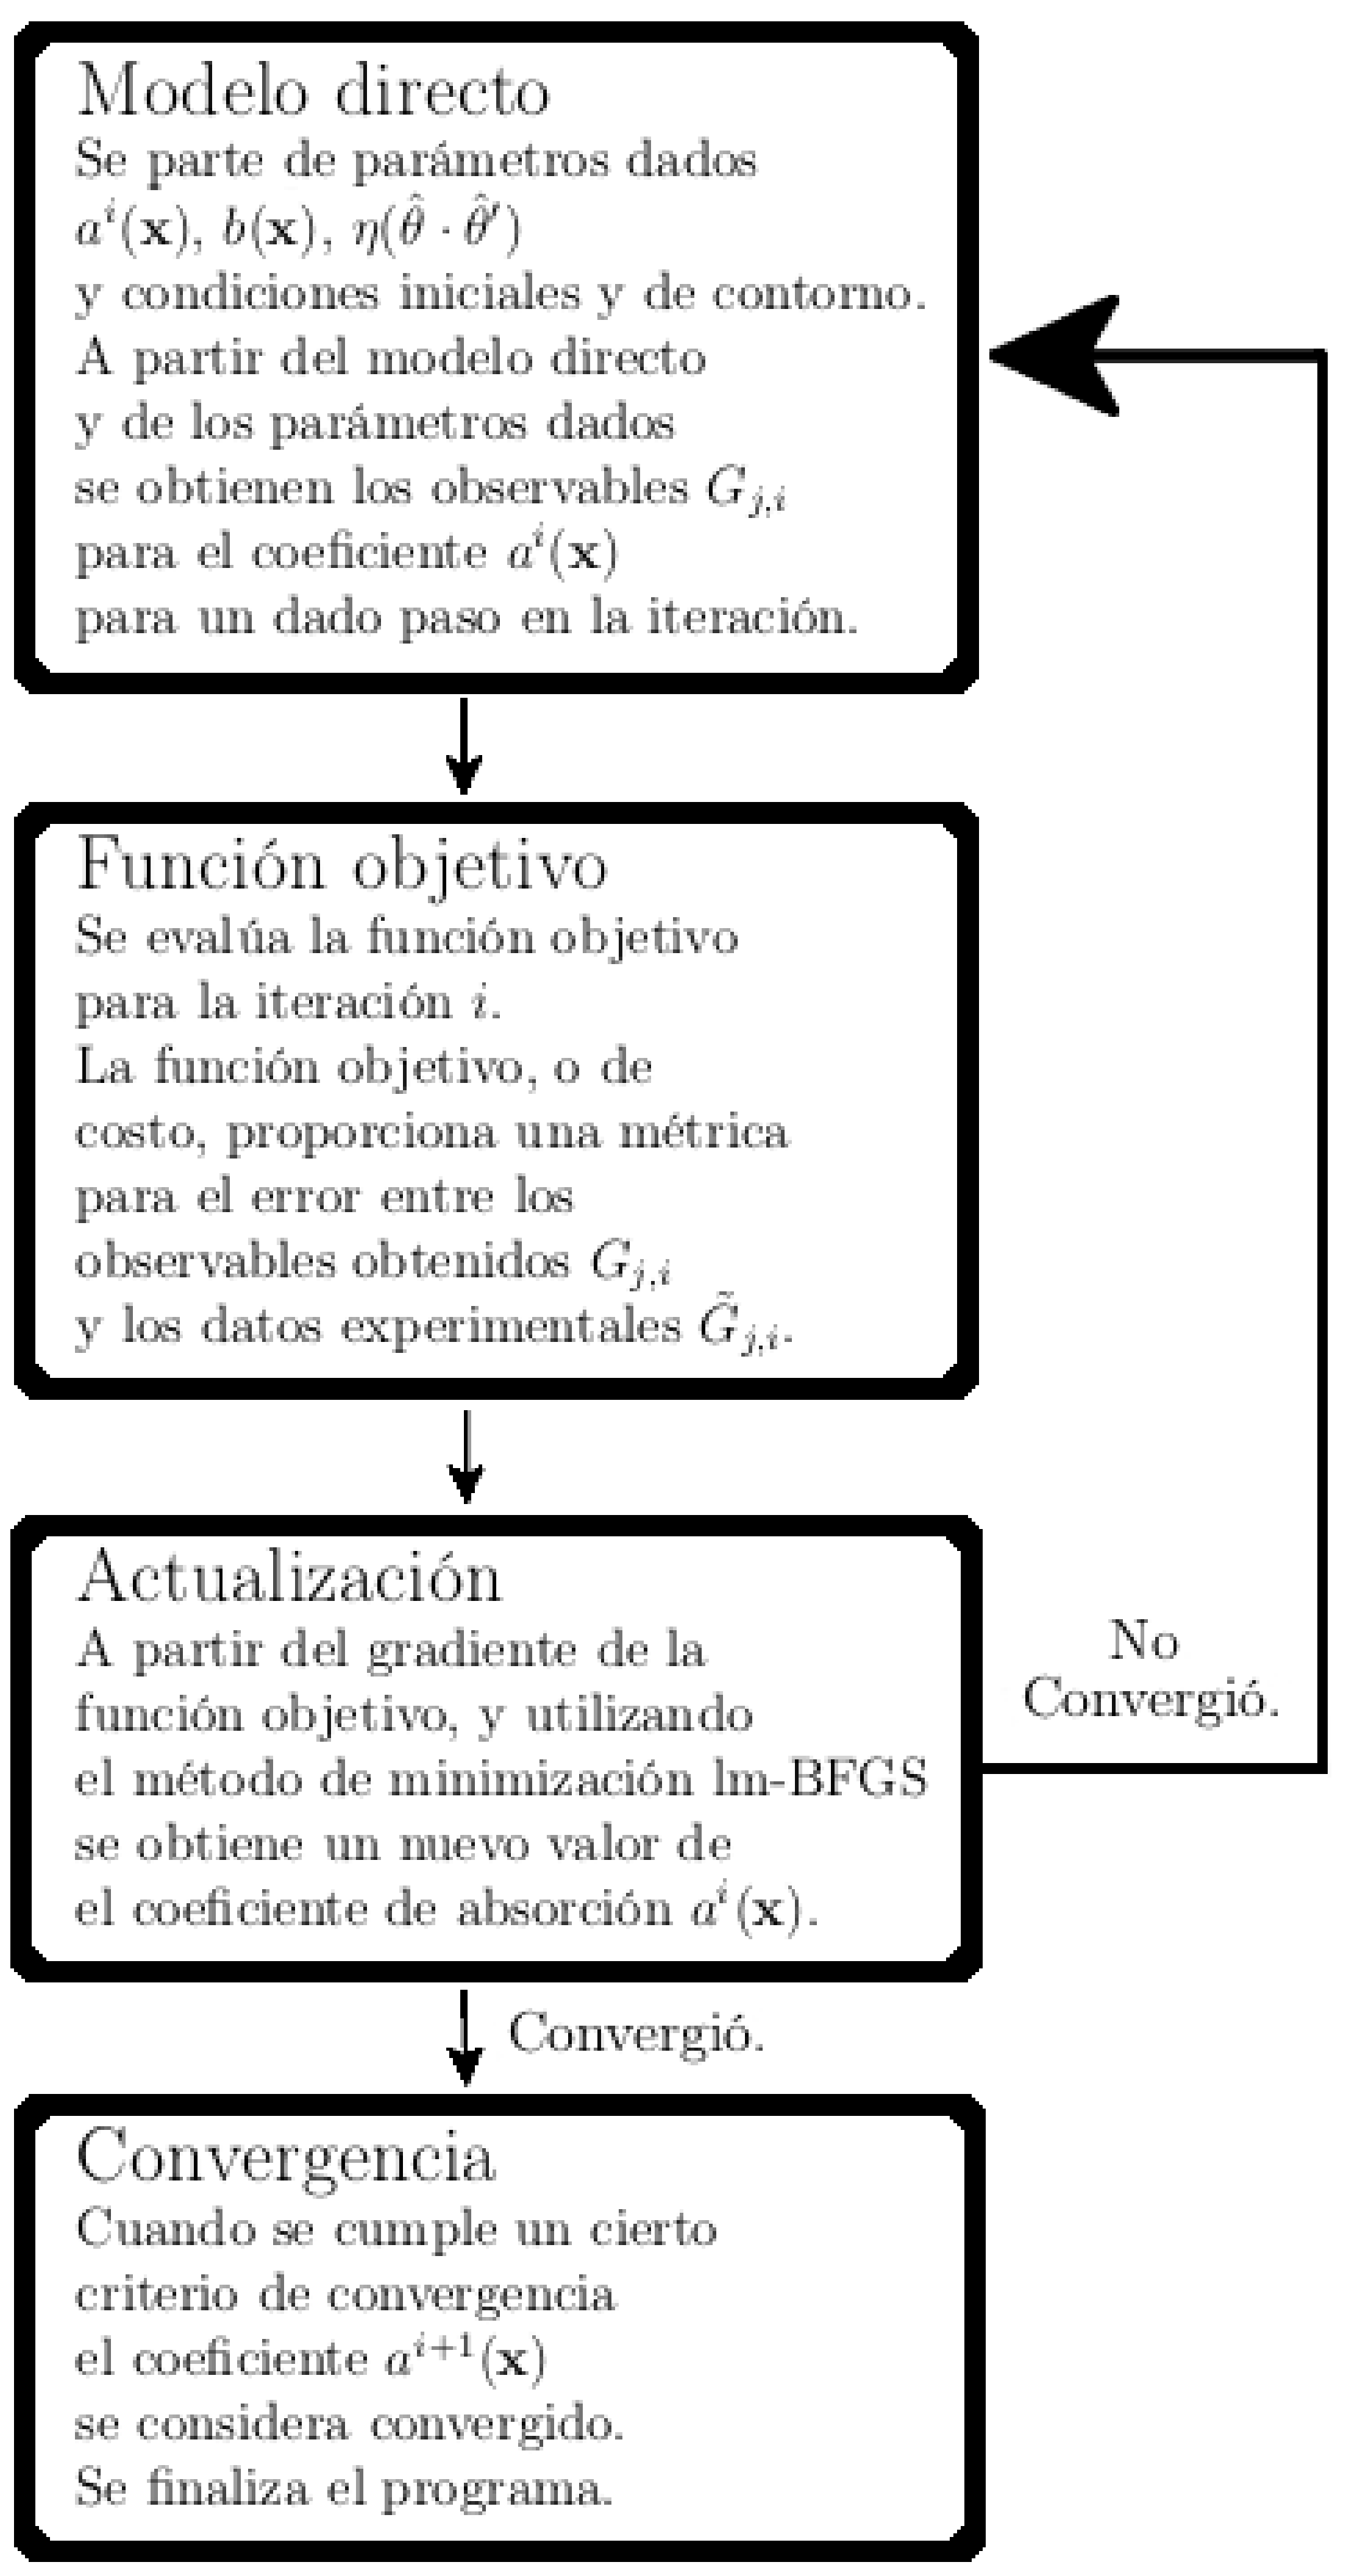
\includegraphics[width=0.48\textwidth]{figuras/mobir.eps}\\
  \caption{Esquema  MOBIR. El modelo directo es utilizado para obtener los observables simulados. Se evalúa el error entre los datos experimentales y los simulados por medio de la función objetivo. 
  Luego, utilizando un método de minimización, se actualiza el coeficiente $a(\x)^{i+1}$ a 
  ser utilizado en la iteración subsiguiente, hasta cumplir 
  un cierto criterio de convergencia. }
 \label{fig:mobir}
\end{wrapfigure}

En este tesis desarrollamos un algoritmo tipo MOBIR~\cite{Hielscher1999,Kim2010} (del inglés, {\em Model Based Iterative Image  
Reconstruction}). Este tipo de esquemas se basan en un modelo físico, y un método de minimización 
iterativo para la reconstrucción del parámetro deseado en el problema inverso.

El modelo físico utilizado es la Ecuación de Transporte Radiativo~\eqref{eq:RTE}. 
Para la minimización del funcional objetivo (que será introducido en una sección posterior) emplearemos el método de minimización 
de Broyden–Fletcher–Goldfarb–Shanno (BFGS) con uso de memoria reducido 
(lm-BFGS, de su sigla en inglés)~\cite{Byrd1995}. 

El problema inverso en tomografía óptica es resuelto como un problema de optimización 
no lineal. A partir de un valor inicial para el coeficiente de absorción $a(\x)^0$, 
el coeficiente de absorción es buscado de forma iterativa, actualizando su valor 
en cada iteración mediante el método lm-BFGS, el cual es un caso particular 
de los métodos de cuasi-Newton~\cite{Nocedal2006,Klose2003QN,Ren2006}. 
Partiendo del valor inicial $a^0(\x)$, el cual en general es estimado 
a partir de información obtenida de manera previa por otros métodos de imagenes, 
el coeficiente de absorción es 
\clearpage
\noindent actualizado en cada paso de la iteración $i+1$, según~\cite{Klose2003QN}
\begin{equation}
\mathbf{a}^{i+1}(\x)=\mathbf{a}^{i}(\x)+\alpha^i  \mathbf{d}^i(\x)
\label{eq:update}
\end{equation}
donde $\mathbf{a}^{i}(\x)$ debe ser interpretado como el 
vector obtenido a partir de el coeficiente de absorción en el 
dominio espacial $\Omega$  
discretizado, con $\alpha^i$ el largo del paso de Newton (que lo consideraremos 
en general $\alpha^i=1$), y $\mathbf{d}^i(\x)$ 
la dirección de descenso. En el caso del método de Newton (o {\em steepest descent}), la dirección de 
descenso vendrá dada por el gradiente $\mathbf{d}^i=-\nabla_a $ de la función objetivo $g$ (que será definida posteriormente). 
En el contexto de esta tesis emplearemos el método lm-BFGS, ya que este método a 
mostrado ser eficiente en el contexto de tomografía óptica~\cite{Klose2003QN,Ren2006,
Prieto2017}. 

\section{El método de minimización BFGS}
\label{sec:BFGS}
Siguiendo a Nocedal~\cite{Nocedal2006}, el método BFGS parte de considerar la expansión de Taylor a segundo orden de la función objetivo 
que buscamos minimizar, la cual estará evaluada para el coeficiente $\mathbf{a}(\x)$,  
lo notaremos, por simplicidad  $g[\mathbf{a}]$

\begin{equation}
g[\mathbf{a}^i+ \mathbf{d}^i]\approx g[\mathbf{a}^i]+ (\mathbf{d}^i)^T \nabla_a g[\mathbf{a}^i]+\frac{1}{2}(\mathbf{d}^i)^T \nabla_a^2 g[\mathbf{a}^i+t\mathbf{d}^i] \mathbf{d}^i=m(\mathbf{d}^i).
\label{eq:Taylor}
\end{equation}
donde $t \in (0,1)$, y $(\mathbf{d}^i)^T$ indica el vector traspuesto a $\mathbf{d}^i$.
Además, si $g$ es al menos dos veces diferenciable se cumple qué 
\begin{equation}
\nabla_a g[\mathbf{a}^i+ \mathbf{d}^i]\approx \nabla_a g[\mathbf{a}^i]+\int_0^1\nabla_a^2 g[\mathbf{a}^i+t\mathbf{d}^i] \mathbf{d}^idt 
\label{eq:Taylor2}
\end{equation}
para algún $t \in (0,1)$.
Exigiendo que se anule la derivada de $m(\mathbf{d^i})$, se llega la dirección de Newton, dada por
\begin{equation}
\mathbf{d}^i=-(\nabla_a^2 g^i )^{-1} \nabla_a g^i.
\label{eq:direccion}
\end{equation}
El principal obstaculo para la aplicación de la dirección de Newton es la 
necesidad de calcular la inversa del Hessiano de la función objetivo, $\nabla_a^2 g^i$, 
lo cual en tomografía óptica, debido a la alta dimensionalidad de la ETR, puede 
resultar extremadamente costoso. 

Por este motivo, el método BFGS implementa una aproximación del Hessiano de la función objetivo (mas concretamente, 
a la inversa del Hessiano) que 
es actualizada a cada paso de la iteración. Sumando y restando el término $ \nabla_a^2 g \mathbf{d}^i$ en la ecuación~\eqref{eq:Taylor2} se llega a
\begin{equation}
\nabla_a g[\mathbf{a}^i+ \mathbf{d}^i]\approx \nabla_a g[\mathbf{a}^i]+ \nabla_a^2 g[\mathbf{a}^i]\mathbf{d}^i + \int_0^1   \left( \nabla_a^2 g[\mathbf{a}^i+t\mathbf{d}^i]-\nabla_a^2 g[\mathbf{a}^i] \right)\mathbf{d}^idt
\label{eq:Taylor3}
\end{equation}
Dado que se asume la continuidad de $\nabla_a g$, el término de la integral 
es $o(||\mathbf{a}^{i+1}-\mathbf{a}^{i}||)$. Tomando $\mathbf{d}^i=\mathbf{a}^{i+1}-\mathbf{a}^{i}$ se llega a la relación
\begin{equation}
\begin{split}
\begin{aligned}
\nabla_a g[\mathbf{a}^{i+1}] &\approx \nabla_a g[\mathbf{a}^i]+ \nabla_a^2 g[\mathbf{a}^{i+1}-\mathbf{a}^i]  + o(||\mathbf{a}^{i+1}-\mathbf{a}^{i}||).\\
\therefore \nabla_a^2 g[\mathbf{a}^{i+1}-\mathbf{a}^i]& \approx \nabla_a g[\mathbf{a}^{i+1}]  - \nabla_a g[\mathbf{a}^{i}].
\end{aligned}
\end{split}
\label{eq:Taylor4}
\end{equation}
Esta última relación nos permite aproximar el Hessiano utilizando las derivadas de 
la función objetivo obtenidos para dos iteraciones sucevias. 
La inversa del Hessiano de la función objetivo es aproximada exigiendo que se cumpla la última relación en~\eqref{eq:Taylor4}, que puede escribirse 
\begin{equation}
(B^{i+1})^{-1}y^i=s^i,
\label{eq:Taylor5}
\end{equation}
con $s_i=  \mathbf{a}^{i+1}-\mathbf{a}^{i}$ y $y^i=\nabla_a g[\mathbf{a}^{i+1}]  - \nabla_a g[\mathbf{a}^{i}]$. La fórmula BFGS para actualizar el Hessiano en cada iteración viene dada por~\cite{Nocedal2006}
\begin{equation}
(B^{i+1})^{-1}=(V^i)^T (B^{i})^{-1}V^i + \rho^i s^i (s^i)^T  ,
%B^{i}-\frac{B^{i}s^i (s^i)^T B^i }{(s^i)^TB^i s^i}+ \frac{y^i (y^i)^T}{(y^i)^T s^i}
\label{eq:HBFGS}
\end{equation}
la cual cumple la relación~\eqref{eq:Taylor5}, donde $\rho^i=\frac{1}{(y^i)^T s^i}$ 
y $V^i=\id - \rho^i y^i (s^i)^T$. 
La dirección de descenso, finalmente, se obtiene de la ecuación~\eqref{eq:direccion} reemplazando 
el Hessiano por su aproximación $B^i$
\begin{equation}
\mathbf{d}^{i}=-(B^{i})^{-1} \nabla_a g[\mathbf{a}^i]. 
\label{eq:HBFGS2}
\end{equation}

\subsection{El método de uso de memoria limitada lm-BFGS}
\label{sec:lmBFGS}
En nuestro algoritmo para la resolución del problema inverso, el coeficiente 
de absorción es actualizado en cada iteración utilizando la relación 

\begin{equation}
\mathbf{a}^{i+1}(\x)=\mathbf{a}^{i}(\x)-(B^{i})^{-1} \nabla_a g[\mathbf{a}^i]
\label{eq:update2}
\end{equation}
Debido a que la aproximación a la inversa del Hessiano, $(B^i)^{-1}$, en tomografía óptica es una matriz 
que para el problema 2D discretizado, con $N_x \times N_y$ puntos 
por cada coordenada espacial tendrá dimensiones  $B^i\in \mathbb{R}^{N_x \times N_y}$, 
la manipulación y almacenamiento de esta matriz puede ser sumamente costosa. Por ello, 
para evitar la manipulación y el almacenamiento de esta matriz, se utiliza 
una versión aproximada de $(B^i)^{-1}$, para la cual se almacenan los vectores $\{s^k, y^k\}$, 
$k=i-m,...,i-1$ para un dado número de puntos $m$ previos a la iteración $i$-esima. 
Para esto se utiliza una aproximación inicial al Hessiano $(B^i)^{-1}_0$
\begin{equation}
(B^i)^{-1}_0=\gamma^i \id,\quad \quad \gamma^i=\frac{(s^{i-1})^T y^{i-1}}{(y^{i-1})^Ty^{i-1}},
\label{eq:initHess}
\end{equation}
y utilizando la ecuación~\eqref{eq:HBFGS} se tiene la relación de recurrencia
\begin{equation}
\begin{split}
\begin{aligned}
(B^{i+1})^{-1}=&(V^{i-1})^T...V^{i-m})^T) (B^i)^{-1}_0 (V^{i-m}...V^{i-1})  \\
&+\rho^{i-m} (V^{i-1})^T...V^{i-m+1})^T)s^{i-m} (s^{i-m})^T(V^{i-m+1}...V^{i-1+1}) \\
&+\rho^{i-m+1} (V^{i-1})^T...V^{i-m+2})^T)s^{i-m+1} (s^{i-m+1})^T(V^{i-m+2}...V^{i-1}) \\
&+...\\
&+\rho^{i-1} s^{i-1} (s^{i-1})^T. 
\end{aligned}
\end{split}
\label{eq:HBFGSrec}
\end{equation}
de donde se tiene el algoritmo~\eqref{algbfgs}~\cite{Byrd1995,Nocedal2006}

\begin{algorithm}
\caption{lm-BFGS}\label{algbfgs}
\begin{algorithmic}[1]
\State dados $m$, $\mathbf{a}^i$, y $\nabla_a g[\mathbf{a}^i]$
\State  $q = \nabla_a g[\mathbf{a}^i]$
\State \textbf{para} $k=i-1,i-2,\ldots,i-m$ hacer 
\State \hskip 0.75em $\alpha^k  = \rho^k (s^k)^T q$,
\State \hskip 0.75em $q  = q- \alpha^k y^k$,
\State \textbf{terminar}
\State $r = (B_0^k)^{-1} q$,
\State \textbf{para} $k=i-m,i-m+1,\ldots,i-1$ hacer 
\State \hskip 0.75em $\beta  = \rho^k (y^k)^T r$,
\State \hskip 0.75em $r  = r+s^k(\alpha^k-\beta)$,
\State \textbf{terminar}
\State Finalizar programa, con $(B^k)^{-1}\nabla_a g[\mathbf{a}^k]=r$.
\end{algorithmic}
\end{algorithm}  
  
En esta tesis utilizaremos el algoritmo lm-BFGS para encontrar 
el mínimo de la función objetivo. En todos los casos, usaremos el valor 
de $m=5$, y se parte de un coeficiente inicial $a^0(\x)$ dado 
por cierto conocimiento obtenido previamente, como puede ser la imagen 
de resonancia magnética de un cuello humano utilizada en la sec.~\ref{sec:inverseres}.
Adicionalmente, es posible incluir cotas para el coeficiente 
de absorción que deseamos reconstruir, de forma tal que 
el proceso de minimización sea realizado 
en un subespacio tal que $a^l(\x)\leq a^i(\x) \leq a^u(\x)$, de forma 
tal que el coeficiente de absorción, para cada punto espacial $\x$ se encuentre 
restringido por las cotas inferior $a^l(\x)$ y superior $a^u(\x)$. Esto restringe el espacio de soluciones posibles, permitiendo explotar información a priori obtenida por otros métodos de imágenes. 
Una condición física que debe cumplirse siempre es que la cota inferior 
para el coeficiente de absorción cumpla $a^l(\x)\geq 0$. Similarmente, 
se conocen cotas superiores para el coeficiente de absorción, y además, 
puede utilizarse los valores conocidos de $a(\x)$ como cotas sobre 
aquellos tejidos donde se sabe que la inclusión no puede ocurrir, 
o si, por la naturaleza del diagnóstico que se está realizando, 
se espera que una dada inclusión 
se encuentre dentro de cierto tipo de tejido, restringiendo mediante cotas 
la reconstrucción para que ocurra dentro del tejido esperado, fijando los 
valores para el resto de los tejidos, como puede ser, la existencia de 
una región de absorción y dispersión nula en la traquea para el cuello 
humano, o las regiones óseas para el caso en el que se intenta dar un diagnóstico 
para un tipo de tumor específico, como lo puede ser para el cáncer de tiroides, 
donde se sabe que el tumor se encontrará localizado en el tejido blando. 
El procedimiento por el cual se imponen dichas cotas en los coeficientes 
puede encontrarse en la ref.~\cite{Byrd1995}. 

\section{El operador de transporte y otras definiciones preliminares}
En esta sección, haremos uso del operador de transporte, el cual definimos
según
\begin{equation}
\begin{split}
\mathcal{T}[u]=\frac{1}
{c}\frac{\partial \ut}{\partial t} + \hth \cdot \nabla \ut&+a(\x)\ut\\
&+b(\x)\left[\ut - \int_{S^1}\eta(\hth\cdot\hth ') u(\x,\hth',t) d\theta'\right],
\end{split}
\label{eq:Toper}
\end{equation}
donde se hizo explícita la dependencia del operador de transporte $\mathcal{T}$ 
con respecto a $\ut$. 

Consideramos el problema ETR de valores iniciales y condiciones 
de contorno
\begin{equation}
\begin{split}
\begin{aligned}
&\mathcal{T}\big[u\big]=0, \;  (\x,\hth)  \in \Omega\times S^1\\
&u(\x,\hth,t=0)=0, \;  (\x,\hth)  \in \Omega\times S^1 \\
&u(\x,\hth,t)=f(\hth \cdot \hnu) u(\x,\hth_r,t) + q(\x,\hth,t) , \; (\x,\hth) \in \Gamma_-
\end{aligned}
\end{split}
\label{eq:RTEt}
\end{equation}
donde todas las cantidades fueron definidas en la sección~\ref{sec:ETR}.


Para concluir esta sección, mencionamos la ``función ventana''~\cite{Bruno2014}
\begin{equation}
\begin{aligned}
\begin{split}
w(v)=
\begin{cases}
  1 &\text{for} \, \, v = 0, \\
       \exp{\left(\frac{2e^{-1/|v|}}{|v|-1}\right)} & \text{for} \, \, 0 < |v| < 1, \\
       0 &\text{for} \, \, |v| \geq 1.
     \end{cases}
\end{split}
\end{aligned}
\label{eq:sourcelabwind}
\end{equation}
de la variable real $v$, la cual se anula para $|v|\geq 1$ y realiza 
una transición suave a uno en el intervalo $-1 < v < 1$. Esta función 
será utilizada de diferentes formas en las secciones subsiguientes---
incluyendo el modelado del perfil temporal y ángular de los pulsos láser, 
así como el modelado de la sensibilidad espacial de los fotodetectores.
\begin{figure}[h!]
\centering
  \includegraphics[width=0.5\linewidth]{figuras/windowed.eps}
  \caption{Grafico de la función ventana $w(v)$~\eqref{eq:sourcelabwind} utilizada 
  para modelar los perfiles temporales y ángular de las fuentes láser, 
  así como la sensibilidad espacial de los fotodetectores.}
 \label{fig:window}
\end{figure}


\section{El método de Fuentes Múltiples Superpuestas}
\label{sec:FMS}
El problema inverso en tomografía óptica en el dominio temporal, es ubicuamente resuelto utilizando el denóminado ``método de barrido'' (MB), del inglés, ``Transport Sweep''. En éste método, se requiere la resolución de un problema directo y un problema adjunto 
para cada fuente $q_i(\x,\hth,t)$, $i=1,\ldots,N_q$ en la ecuación~\eqref{eq:RTEt}, 
con $N_q$ el número total de fuentes empleadas. 
El mayor inconveniente que encuetra este método es que el costo computacional 
incrementa linealmente con el número de fuentes utilizadas. En general, 
cada fuente permite sensar diferentes partes del dominio espacial en consideración. 
Dado que la intensidad lumínica de las fuentes laser empleadas sufre una 
atenuación de tipo exponencial, debido a la absorción y a la dispersión 
en el interior del medio participante, en general se requiere la utilización de 
fuentes múltiples. Debido a la atenuación exponencial de la intensidad lumínica, 
en general, la iluminación entre fuentes lejanas no suele afectarse entre sí. 
Motivados por este hecho en esta tesis introducimos un método de Fuentes Múltiples 
Simultáneas (FMS). Este método se vale del uso de ``fuentes generalizadas'', 
las cuales pueden representar una o múltiples fuentes láser, las cuales 
pueden ser activadas, con ciertos retrasos temporales, de forma superpuesta 
en un único problema directo, lo que brinda ventajas en el costo computacional 
que serán demostradas mas adelante.  

Los métodos MB y FMS se basan en el uso de dos tipos diferentes de fuentes, 
donde ambas pueden expresarse como
\begin{equation}
  q = q_i(\x,\hth,t) =\sum_{k=1}^{N_s} s_{k,i}(\x,\hth,t) ,\quad i=1,2,\ldots,N_q
\label{eq:RTEsources}
\end{equation}
para ciertos valores enteros de $N_q$ y $N_s$. Utilizando la 
función ventana~\eqref{eq:sourcelabwind}, definimos
\begin{equation}
  s_{k,i}(\x,\hth,t) = \exp(-|\x-\x_{k,i}|^2/
  2\sigma_\x^2)w(\beta_{k,i})w(\gamma_{k,i}),
\label{eq:RTEsources2}
\end{equation}
para las posiciones de las fuentes láser $\x_{k,i}\in\partial\Omega$, 
con el diámetro de la iluminación láser sobre la superficie del dominio $\partial \Omega$ 
siendo $\sigma_\x$, y la distribución 
ángular $\beta_{k,i}=|\theta-\theta_{k,i}|/\sigma_{\theta}$, 
donde $\theta_{k,i}$ ($0\leq \theta_{k,i} < 2\pi$) y $\sigma_{\theta}$
modelan el ángulo para la dirección $\hth_{k,i}$ en la que apunta el láser 
y la distribución ángular de la radiación para el láser $(k,i)$-ésimo, respectivamente. 
Similarmente, $\gamma_{k,i}=|t-\tau_{k,i}|/\sigma_t$, modela el pulso 
láser, con retardos temporales $\tau_{k,i}\geq 0$ para diferentes fuentes láser, 
y donde $\sigma_t$ denota la mitad de la duración total del pulso láser. 

Para las fuentes en el método MB fijamos $N_s=1$ y, en general, $N_q>1$ 
(se utiliza una secuencia de $N_q>1$ fuentes láser, requiriendo la resolución de 
$N_q$ pares de problemas directos y adjuntos por cada iteración en el problema inverso), 
mientras que en el método FMS propuesto, utilizamos $N_s>1$ y $N_q=1$ (de forma 
que $N_s>1$ fuentes laser son superpuestas en una única ``fuente generalizada'', 
requiriendo por lo tanto la resolución de un único par de problemas directo y 
adjunto por iteración para la resolución del problema inverso). En cada ``barido''
del método MB cada una de las $N_q>1$ fuentes laser es aplicada de forma 
independiente de las otras, con todos los retardos temporales $\tau_{i,1}=0$ ($1\leq i\leq N_q$), y se guardan los valores registrados por todos los fotodetectores utilizados~\cite{Prieto2017,Dorn}. En el método FMS propuesto, en cambio, 
se utiliza una única fuente generalizada ($N_q=1$), la cual incorpora 
las contribuciones de las $N_s>1$ fuentes laser alrededor de $\partial \Omega$, 
con retardos temporales $\tau_{1,k}\geq 0$. Debido a los retardos temporales 
utilizados, en el método FMS se requieren simulaciones mas largas para la resolución de los problemas directo y adjunto, en comparación con las simulaciones requeridas 
para cada una de las $N_q>1$ fuentes en el método MB. Sin embargo, como se 
demuestra en la sección~\ref{sec:inverseres}, la estrategia de fuentes simultaneas 
permite obtener ganancias significativas en términos del costo computacional 
total para todo el proceso de inversión, sin detrmiento en la precisión de la 
reconstrucción obtenida. 

\section{La función objetivo y el formalismo del método adjunto para el cálculo de su gradiente}

Tanto el método MB como el método FMS se basan en el uso de  $N_d\geq 1$ detectores, 
donde el detector $j$-ésimo ($1\leq j\leq N_d$) ubicado en el punto 
$\x_j \in \partial \Omega$, queda caracterizado por el operador 
de medición $G_j=G_j[u](t)$ definido como 
\begin{equation}
  G_j[u]=\oint_{\partial \Omega}\int_{\hth \cdot \hnu>0}[1-f(\hth
  \cdot \hnu)]
  \hth \cdot \hnu 
  \times w\left( \frac{ |\x-\x_j |}{\sigma_d} \right) \ut
  d\theta dS
\label{eq:OpMed}
\end{equation}
para cualquier función $\ut$ definida en $(\x,\hth,t)\in\Omega\times S^1 \times [0,T] $. 
Utilizando la función~\eqref{eq:sourcelabwind}, y llamando $\sigma_d>0$ 
al área efectiva de los detectores, el factor $w( |\x-\x_j |/\sigma_d) $ 
caracteriza la sensibilidad espacial del detector $j$-ésimo, 
y $dS$ denota el elemento de área en $\partial \Omega$. 
Claramente, el operador de medición $G_j[u]$ cuantifica el flujo de fotones 
transmitidos a través de la superficie del detector. Para cada 
fuente generalizada $q_i$ tenemos un número $N_d$ de detecciones 
resueltas en el tiempo. El número y la ubicación de los detectores 
permanecen fijos durante el proceso de inversión. 

En vista de las consideraciones hechas previamente en la sección~\ref{sec:inverso}, 
en lo que sigue haremos explícita la dependencia del operador de transporte 
$\mathcal{T}$ y de la solución $u$ en la ecuación~\eqref{eq:Toper} 
con respecto al coeficiente de absorción $a=a(\x)$ , llamando 
\begin{equation}\label{eq:Toper_a}
  \mathcal{T}[u] = \mathcal{T}[u,a]= \mathcal{T}[u,a](\x,\hth,t)
\end{equation}
y
\begin{equation}\label{u_of_a}
  u=u[a]=u[a](\x,\hth,t),
\end{equation}
respectivamente.

Expresamos el problema inverso para el parámetro óptico  $a(\x)$ 
en términos del problema de minimización de la función objetivo
\begin{equation}
  \Lambda[a]=\sum_{i=1}^{N_q} g_i[u_i],
\label{eq:FObjpr}
\end{equation}
donde, para un dado coeficiente de absorción $a$,
\begin{equation}\label{ui_of_a}
  u_i = u_i[a] = u_i[a](\x,\hth,t)
\end{equation}
denota la solución $u=u_i$ de la ecuación~\eqref{eq:RTEt} con $q=q_i$ 
(donde se incluyó un detalle creciente de derecha a izquierda en la ecuación~\eqref{eq:FObjpr}
concerniente a la dependencie de $u_i$ en $a$, y las variables espaciales, angular y temporal), 
y donde, para un dado número de mediciones $N_q \times N_d$ en los detectores $\tilde{G}_{j,i}$ 
($N_d$ detecciones $\tilde{G}_{j,i}$ para cada una de las $N_q$ fuentes generalizadas $q_i$) 
y utlizando la ecuación~\eqref{eq:OpMed}, $g_i$ denota la funcional 
\begin{equation}
  g_i[u] = \frac{1}{2} \sum_{j=1}^{N_d} \int_0^T (G_j[u]-\tilde
  {G}_{j,i})^2 dt.
\label{eq:FObj}
\end{equation}
Para minimizar la función objetivo~\eqref{eq:FObjpr} utilizamos el algorítmo 
de descenso por gradiente 
lm-BFGS (ver ref.~\cite{Byrd1995} y secciones~\ref{sec:BFGS} y~\ref{sec:lmBFGS}), 
el cual se basa en el uso de la derivada funcional $\frac{d\Lambda}{da} [a;\delta a]$ 
con respecto al coeficiente de absorción $a = a(\x)$ en la dirección $\delta a$. 
Aquí notamos $\frac{d}{da}$ a la diferenciación de Gateaux~\cite{Hille1974}: 
para una dada función $a= a(\x)$ y una dada poerturbación $\delta a= \delta a(\x)$, 
la derivada de Gateaux de una dada funcional $h = h[a]$ en la dirección $\delta a$ 
se define según
\begin{equation}\label{gateaux}
  \frac{dh}{da}[a; \delta a ] = \lim_{\varepsilon \to 0} \frac{h[a +\varepsilon \delta a]
    - h[a]}{\varepsilon}.
\end{equation}
Puede darse una definición similar para las derivadas parciales de Gateaux 
de un operador $w = w[a](\x,\hth,t)$ (como, \eg, el operador~\eqref{eq:Toper}, 
la solución $u = u[a]=u[a](\x,\hth,t)$ a la ecuación~\eqref{eq:RTEt},etc.):
\begin{equation}\label{gateaux_part}
  \frac{\partial w}{\partial a}[a; \delta a ](\x,\hth,t) = \lim_{\varepsilon \to 0} \frac{w[a +\varepsilon \delta a](\x,\hth,t)
    - w[a](\x,\hth,t)}{\varepsilon}.
\end{equation}
En lo que sigue, utilizamos las derivadas de Gateaux para la composición 
de funcionales y operadores, para los cuales se satisface la regla de la cadena. 
Por ejemplo, para la composición  $h\circ w [a] = h\big[w[a]\big]$ 
se tiene la deintidad de la regla de la cadena
\begin{equation}\label{eq:chain}
  \frac{d (h\circ w)}{da} \big[a;\delta a\big]= \frac{d h}{
    d w}\left[w[a];\frac{\partial w}{\partial a} \big[a;\delta
    a\big]\right].
\end{equation}
En nuestro contexto, podemos ilustrar esta relación como sigue. 
Al considerar una perturbación $\varepsilon$ por la función $\delta a = \delta a(\x)$ 
del coeficiente $a$, resulta el coeficiente perturbado $(a+\varepsilon\delta a)$, 
de donde se tiene el operador perturbado $w[a+\varepsilon\delta a]$ (en nuestro caso, 
el operador perturbado puede ser \eg la solución $w[a+\varepsilon\delta a]$ del problema~\eqref{eq:RTEt} perturbado con coeficiente de absorción $(a+\varepsilon\delta a)$; 
cf. ec.~\eqref{u_of_a}.) Utilizando la definición de la derivada 
de Gateaux~\eqref{gateaux_part} obtenemos
\[
  w[a+\varepsilon\delta a] = w[a]+\varepsilon \frac{\partial
    w}{\partial a}[a; \delta a ] + o(\varepsilon)
\]
donde $\frac{o(\varepsilon)}{\varepsilon}\to 0$ para $\varepsilon\to 0$. 
En otras palabras, el error en la aproximación $w[a+\varepsilon\delta a] \approx w[a]+\varepsilon \frac{\partial
  w}{\partial a}[a; \delta a ]$ es mucho mas pequeño que $\varepsilon$. 
Por lo tanto, puede aproximarse   
\[
  h\big[w[a+\varepsilon\delta a]\big] \approx h\left[w[a]+\varepsilon \frac{\partial
    w}{\partial a}[a; \delta a ]\right]
\]
en el cociente incremental, de la forma~\eqref{gateaux_part}, 
para la derivada de la función compuesta $h\big[w[a]\big]$, 
de donde resulta 
\[
 \lim_{\varepsilon\to 0}\frac{h\big[w[a+\varepsilon\delta a]\big]
     -h\big[w[a]\big]}{\varepsilon}  = \lim_{\varepsilon\to
    0} \frac{h\big[w[a]+\varepsilon \frac{\partial w}{\partial a}[a;
    \delta a ]\big]-h\big[w[a]\big]}{\varepsilon},
\]
y, por lo tanto, claramente, el lado derecho de~\eqref{eq:chain} $\blacksquare$.

La derivada funcional de la función objetivo~\eqref{eq:FObjpr} viene 
dada por
\begin{equation}
  \frac{d \Lambda}{da} = \sum_{i=1}^{N_q} \frac{d (g_i\circ
    u_i)}{da}[a;\delta a].
\label{eq:Gradsumq}
\end{equation}
Para obtener las derivadas de la suma del lado derecho 
de esta ecuación aplicamos la regla de la cadena~\eqref{eq:chain}, 
de donde resulta  
\begin{equation}
\frac{d (g_i\circ u_i)}{da}[a;\delta a] = \frac{d g_i}{
    d u}\left[u_i[a];\frac{\partial u_i}{\partial a} \big[a;\delta
    a\big]\right],
  \label{eq:AdjointMEthod}
\end{equation} 
o, utilizando~\eqref{eq:OpMed} y~\eqref{eq:FObj}, $\frac{d (g_i\circ u_i)}{da}[a;\delta a]=\mathcal{G}[a;\delta a]$ donde
\begin{equation}
\begin{split}
\begin{aligned}
  \mathcal{G}[a;\delta a]\coloneqq 
  \int_0^T \oint_{\partial \Omega} \int_{\hth \cdot \hnu>0}
  \sum_{j=1}^{N_d} &\left( G_j\big[u_i[a]\big]-
    \tilde {G}_{j,i} \right) [1-f(\hth \cdot \hnu)]\\ 
   &\times \hth \cdot \hnu w\left( \frac{ |\x-\x_j |}{\sigma_d}
  \right) \frac{\partial u_i}{\partial a}[a;\delta a](\x,\hth,t)
  d\theta dS dt.
\end{aligned}
\end{split}
\label{eq:AdjointMEthod2}
\end{equation}
Claramente, en vista de la ecuación~\eqref{eq:AdjointMEthod2}, 
los gradientes~\eqref{eq:Gradsumq} necesarios para la estrategia 
de minimización en un contexto discreto podrían generarse 
evaluando y substituyendo en esta ecuación la derivada 
$\frac{\partial u_i}{\partial a}[a;\delta a]$, para cada $a$ 
discretizado en el proceso de minimización mediante el algorítmo lm-BFGS. 
Sin embargo, la evaluación de estas derivadas parciales utilizando, 
por ejemplo, un esquema de diferencias finitas, requiere la evaluación 
de una solución al problema de transporte~\eqref{eq:RTEt} para 
cada dirección $\delta a$, lo cual claramente constituye 
un costo computacional inabordable para cualquier problema realista. 
Para evitar este costo computacional nos basamos en la 
estrategia del método adjunto, que se describe a continuación.

Para evaluar la derivada de la ec.~\eqref{eq:AdjointMEthod2} de forma eficiente 
debemos eliminar la dependencia en la derivada $\frac{\partial u_i}{\partial a}[a;\delta a]$ 
del lado derecho de dicha ecuación. Como se indica a continuación, 
esto puede lograrse considerando el problema de valores iniciales 
y de contorno, que se obtiene mediante diferenciación, para un coeficiente 
$a$ y en la dirección $\delta a$, de cada una de las tres ecuaciones en 
el problema de valores iniciales y de contorno~\eqref{eq:RTEt}. 
En particular, para la primera línea en~\eqref{eq:RTEt} obtenemos
\begin{equation}
  0 = \frac{d\mathcal{T}}{da}\big[u_i[a],a;\delta a
  \big]=\frac{\partial \mathcal{T}}{\partial u}
  \left[u_i[a],a;\frac{\partial u_i}{\partial a}\big[a;\delta
    a\big]\right] + \frac{\partial \mathcal{T}}{\partial
    a}\big[u_i[a],a; \delta a \big].
\label{eq:RRTEder}
\end{equation}
Pero, por linealidad de $\mathcal{T}$, tenemos qué $\mathcal{T}[u+\varepsilon \frac{\partial u}{\partial a}]=\mathcal{T}[u]+\varepsilon\mathcal{T}[\frac{\partial u}{\partial a}]$ y 
de la definición de la derivada de Gateaux~\eqref{gateaux_part}
\begin{equation}
\begin{split}
\begin{aligned}
\frac{\partial \mathcal{T}}{\partial u}\left[u_i[a],a;\frac{\partial u_i}{\partial a}\big[a;\delta a\big]\right]= \lim_{\varepsilon \to 0} \frac{\mathcal{T}[u_i +\varepsilon\frac{\partial u_i}{\partial a}\big[a;\delta a\big],a]-\mathcal{T}[u_i,a]}{\varepsilon},
\end{aligned}
\end{split}
\label{eq:linealidadT}
\end{equation}
de donde
\begin{equation}
\begin{split}
\begin{aligned}
\frac{\partial \mathcal{T}}{\partial u}\left[u_i[a],a;\frac{\partial u_i}{\partial a}\big[a;\delta a\big]\right]=
\mathcal{T}\left[\frac{\partial u_i}{\partial a}\big[a;\delta a\big],a\right],
\end{aligned}
\end{split}
\label{eq:RRTEdet3}
\end{equation}
y, por lo tanto, de~\eqref{eq:RTEt}, resulta la relación
\begin{equation}
\frac{\partial \mathcal{T}}{\partial a}\big[u_i[a],a;\delta a\big] + 
\mathcal{T}\left[ \frac{\partial u_i}{\partial a}\big[a;\delta a\big],a \right]=0
\label{eq:RRTEdet4}
\end{equation}
Esta relación provee, para cada $(\x,\hth,t)$, una ecuación 
lineal para las dos incógnitas $u_i[a]$ y 
$\frac{\partial u_i}{\partial a}\big[a;\delta a\big]$.

Para eliminar la cantidad $\frac{\partial u_i}{\partial a}[a;\delta a]$ 
en el lado derecho de la ecuación~\eqref{eq:AdjointMEthod2} 
sustraemos a ambos lados de dicha identidad una ``combinación lineal 
con coeficientes apropiados'' $\lambda$  obtenida a partir de la 
relación~\eqref{eq:RRTEdet4}---o, más precisamente, la integral 
en $(\x,\theta,t)\in\Omega\times [0,2\pi)\times [0,T]$
del producto de la relación~\eqref{eq:RRTEdet4} por una función apropiada 
$\lambda (\x,\hth,t)$. (Más abajo también incorporamos ecuaciones adicionales 
relacionadas a las condiciones iniciales y de contorno en la ec.~\eqref{eq:RTEt}).

Por simplicidad notacional, expresamos estas integrales en términos 
del producto escalar 
\begin{equation}\label{scalar}
  \left\langle v,w \right\rangle= \int_0^T\int_{\Omega}\int_{S^1}
  v(\x,\hth,t)w(\x,\hth,t) d\theta d\x dt
\end{equation}
para las funciones $v$ y $w$ de las variables $(\x,\hth,t)$. 
Para una dada función  $\lambda_i =
\lambda_i[a](\x,\hth,t)$ obtenemos de~\eqref{eq:RRTEdet4} 
la ecuación
\begin{equation}
  \left \langle \lambda_i , 
    \frac{\partial \mathcal{T}}{\partial a}[u_i,a; \delta a]
  \right \rangle + \left \langle \lambda_i , 
    \mathcal{T}\left[\frac{\partial u_i}{\partial a}\big[a;\delta a\big],a\right] \right \rangle
  =0,
\label{eq:RRTEdet5}
\end{equation}
para la cual, eligiendo una función $\lambda_i$ apropiada, 
buscamos sustraer este término en la ec.~\eqref{eq:AdjointMEthod2} 
de forma tal de eliminar el término problemático $\frac{\partial u_i}{\partial a}[a;\delta a]$.

Para elegir la función $\lambda_i$ que cumpla la cancelación deseada, 
utilizamos integración por partes para expresar el segundo 
sumando en la ec.~\eqref{eq:RRTEdet5} como una integral del producto 
de dos funciones, una de las cuales es el término $\frac{\partial u_i}{\partial a}$. 
La integración por partes de este segundo sumando da como resultado 
la suma de una integral ``volumétrica'' $\mathcal{A}$ 
(una integral sobre $\Omega\times [0,2\pi)\times [0,T]$) 
mas una suma de términos de ``borde'' $\mathcal{B} +\mathcal{C}$:
\begin{equation}\label{eq:int_parts_termabc}
  \left \langle \lambda_i , \mathcal{T}\left[\frac{\partial
        u_i}{\partial a}\big[a;\delta a\big],a\right] \right \rangle = \mathcal{A} +\mathcal{B} +\mathcal{C}
\end{equation}
donde
\begin{flalign}
\displaystyle \mathcal{A}[a;\delta a]\coloneqq \int_0^T  
\int_{\Omega} \int_{S^1} \frac{\partial u_i}{\partial a}[a;\delta a] \Bigg[-\frac{1}
{c}\frac{\partial \lambda_i}{\partial t} 
- \hth \cdot \nabla \lambda_i+ (a+b)\lambda_i 
- b\int_{S^1}
\eta(\hth\cdot\hth ') \lambda_i d\theta'\Bigg] d\theta  d\x dt,&&
\label{eq:A}
\end{flalign}

\begin{flalign}
\mathcal{B}[a;\delta a]\coloneqq\int_{\Omega}\int_{S^1} \left[\frac{\partial u_i}{\partial a}[a;\delta a] \lambda_i\right]_0^T d\theta d\x &&
\label{eq:B}
\end{flalign}
y
\begin{flalign}
  \displaystyle \mathcal{C}[a;\delta a]\coloneqq\int_0^T
  \oint_{\partial \Omega} \int_{S^1} \hth\cdot \hnu \lambda_i
  \frac{\partial u_i}{\partial a}[a;\delta a] d\theta dS dt.&&
\label{eq:C}
\end{flalign}
Sustrayendo la combinación linear~\eqref{eq:RRTEdet5} de la ec.~\eqref{eq:AdjointMEthod2}
 y utilizando las relaciones~\eqref{eq:int_parts_termabc}-\eqref{eq:C} 
 obtenemos
\begin{equation}
\frac{d (g_i\circ u_i)}{da}[a;\delta a] = 
\mathcal{G} -\mathcal{A} -\mathcal{B} -\mathcal{C}
-\left \langle \lambda_i , 
\frac{\partial \mathcal{T}}{\partial a}[u_i,a;\delta a]
 \right \rangle.
\label{eq:AdjointMEthodIII}
\end{equation}
Claramente, la cantidad $\frac{\partial u_i}{\partial a}$ 
en~\eqref{eq:AdjointMEthodIII} resultara eliminada, 
como es deseado, sí y sólo sí
\begin{equation}
  \mathcal{A} +\mathcal{B} +\mathcal{C} = \mathcal{G},
\label{eq:AdjointMEthod4}
\end{equation}
dado que el último término en el lado derecho de la ec.~\eqref{eq:AdjointMEthodIII} 
no contiene a $\frac{\partial u_i}{\partial a}$. Una 
vez elegida la función  $\lambda_i$ tal que se satisface 
la relación~\eqref{eq:AdjointMEthod4}, y utilizando la derivada de 
Gateaux
\begin{equation}
\begin{split}
\begin{aligned}
 \frac{\partial \mathcal{T}}{\partial a}[u_i,a;\delta a]=\delta a(\x) u_i[a](\x,\hth,t),
\end{aligned}
\end{split}
\label{eq:kdeltalgat}
\end{equation}
de~\eqref{eq:AdjointMEthodIII} resulta la expresión
\begin{equation}
\displaystyle \frac{d (g_i\circ u_i)}{da}[a;\delta a] =
 -\Big \langle \lambda_i[a](\x,\hth,t) , \delta a(\x)  u_i[a](\x,\hth,t) \Big \rangle 
\label{eq:FDwin2}
\end{equation}
para la derivada funcional, la cual no contiene el término desafiante 
$\frac{\partial u_i}{\partial a}$.

Para obtener la solución  $\lambda_i=\lambda_i[a](\x,\hth,t)$ 
a la ec.~\eqref{eq:AdjointMEthod4} notamos que, en vista 
de los dominios de integración espacial en las ecuaciones~\eqref{eq:AdjointMEthod2} 
y ~\eqref{eq:A}-\eqref{eq:C}, la ec.~\eqref{eq:AdjointMEthod4} 
se satisface sí y sólo sí se cumplen 
las condiciones (i)~$\mathcal{A}=0$, (ii)~$\mathcal{B}=0$ y
(iii)~$\mathcal{C}-\mathcal{G}=0$. La condición (i) claramente implica 
que el término en corchetes para~\eqref{eq:A} se anule:
\begin{equation}
-\frac{1}
{c}\frac{\partial \lambda_i}{\partial t} 
- \hth \cdot \nabla \lambda_i+ (a+b)\lambda_i 
- b\int_{S^1}
\eta(\hth\cdot\hth ') \lambda_i d\theta'=0.
\label{condA}
\end{equation}
En lo que sigue, llamaremos al operador que interviene en esta ecuación $\mathcal{T}^*\big[\lambda_i[a],a\big]$.

Para cumplir la condición (ii) imponemos la condición ``final'' $\lambda_i(\x,\hth,t=T)=0$, 
dado que en vista de~\eqref{eq:RTEt}, tenemos qué $\frac{\partial u_i}{\partial a} = 0$ 
para $t=0$. 

El término de borde~(iii), finalmente, requiere 
descomponer la integral~\eqref{eq:C} en dos integrales
$\mathcal{C}_-$ y $\mathcal{C}_+$, 
donde las integrales quedan restringidas a los dominios 
angulares  $\hth\cdot \hnu<0$ y $\hth\cdot \hnu >0$:
\begin{equation}
\begin{split}
\begin{aligned}
  \displaystyle \mathcal{C}[a;\delta a]&=\mathcal{C}_-[a;\delta a] + \mathcal{C}_+[a;\delta a]
  \\&=\int_0^T
  \oint_{\partial \Omega} \left[ \int_{\hth \cdot \hnu<0} \hth\cdot \hnu \lambda_i
  \frac{\partial u_i}{\partial a}[a;\delta a] d\theta + \int_{\hth \cdot \hnu>0} \hth\cdot \hnu \lambda_i
  \frac{\partial u_i}{\partial a}[a;\delta a] d\theta  \right] dS dt.
\end{aligned}
\end{split}
\label{eq:C2}
\end{equation}
Incorporando la condición de contorno de Fresnel que se obtiene 
por diferenciación de la ec.~\eqref{eq:RTEt}, 
$\frac{\partial u_i}{\partial a}(\x,\hth,t)=f(\hth \cdot \hnu)
\frac{\partial u_i}{\partial a}(\x,\hth_r,t)$ ($(\x,\hth) \in \Gamma_-$)  en el término $\mathcal{C}_-$ 
tenemos 
\begin{equation}
\begin{split}
\begin{aligned}
  \displaystyle\mathcal{C}_-[a;\delta a]=\int_0^T
  \oint_{\partial \Omega} \int_{\hth \cdot \hnu<0} \hth\cdot \hnu \lambda_i(\x,\hth,t)
  f(\hth \cdot \hnu) \frac{\partial u_i}{\partial a}(\x,\hth_r,t)[a;\delta a] d\theta  dS dt.
\end{aligned}
\end{split}
\label{eq:C2m}
\end{equation}
dado que el término $\mathcal{C}-\mathcal{G}=0$ involucra dos integrales 
en $\hth\cdot \hnu >0$, buscamos llevar la integral $\mathcal{C}_-$ en $\hth\cdot \hnu <0$
al dominio $\hth\cdot \hnu>0$ mediante el cambio de variable $\hth_r=\R \hth$, 
con $\R$ la matriz de reflexión definida en la sección~\ref{sec:ETR}, y 
donde, dado que para la matriz de reflexión $\R=\R^{-1}$, vale qué $\hth=\R\hth_r$:
\begin{equation}
\begin{split}
\begin{aligned}
  \displaystyle\mathcal{C}_-[a;\delta a]=-\int_0^T
  \oint_{\partial \Omega} \int_{\hth_r \cdot \hnu>0} \hth_r \cdot \hnu \lambda_i(\x,\R \hth_r,t)
  f(\R \hth_r \cdot \hnu) \frac{\partial u_i}{\partial a}(\x,\hth_r,t)[a;\delta a] d\theta_r  dS dt.
\end{aligned}
\end{split}
\label{eq:C2m2}
\end{equation}
sustituyendo la variable muda $\hth_r$ por $\hth$ y usando nuevamente qué $\hth_r=\R \hth$ 
y qué $f(\R \hth \cdot \hnu)=f(\hth \cdot \hnu)$:
\begin{equation}
\begin{split}
\begin{aligned}
  \displaystyle\mathcal{C}_-[a;\delta a]=-\int_0^T
  \oint_{\partial \Omega} \int_{\hth \cdot \hnu>0} \hth \cdot \hnu \lambda_i(\x,\hth_r,t)
  f(\hth \cdot \hnu) \frac{\partial u_i}{\partial a}(\x,\hth,t)[a;\delta a] d\theta  dS dt.
\end{aligned}
\end{split}
\label{eq:C2m3}
\end{equation}
Finalmente, podemos escribir la condición~(iii) $\mathcal{C}-\mathcal{G}=$ cómo
\begin{equation}
\begin{split}
\begin{aligned}
  \displaystyle\mathcal{C}-\mathcal{G}=&\int_0^T
  \oint_{\partial \Omega} \int_{\hth \cdot \hnu>0} \hth \cdot \hnu 
  \frac{\partial u_i}{\partial a}[a;\delta a] \Bigg[  \lambda_i(\x,\hth,t)
    -f(\hth \cdot \hnu)  \lambda_i(\x,\hth_r,t)   \\
    &- \sum_{j=1}^{N_d} \left( G_j\big[u_i[a]\big]-
    \tilde {G}_{j,i} \right) [1-f(\hth \cdot \hnu)]
   \times \hth \cdot \hnu w\left( \frac{ |\x-\x_j |}{\sigma_d}
  \right) 
   \Bigg] d\theta  dS dt=0.
\end{aligned}
\end{split}
\label{eq:cond3}
\end{equation}
la condición~\eqref{eq:cond3} se cumplirá sí y sólo sí 
\begin{equation}
\begin{split}
\begin{aligned}
  \lambda_i(\x,\hth,t)=&
    f(\hth \cdot \hnu) \lambda_i(\x,\hth_r,t) \\
   &+ \sum_{j=1}^{N_d} \left( G_j\big[u_i[a]\big]-
    \tilde {G}_{j,i} \right) [1-f(\hth \cdot \hnu)]
   \times \hth \cdot \hnu w\left( \frac{ |\x-\x_j |}{\sigma_d}
  \right)\; (\x,\hth)\in \Gamma_+.
\end{aligned}
\end{split}
\label{eq:cond4}
\end{equation}

En suma, llamando $\mathcal{T}^*\big[\lambda_i[a],a\big]=-\frac{1} {c}\frac{\partial
  \lambda_i} {\partial t}- \hth \cdot \nabla \lambda_i + (a+b)\lambda_i-
b\int_{S^1}\eta(\hth\cdot\hth ') \lambda_i d\theta'$, hemos 
demostrado que se cumplirán las condiciones~(i), (ii) y~(iii) sí se eligen 
los ``coeficientes'' $\lambda_i$ de forma tal que sea solución 
del problema adjunto
\begin{equation}
\begin{split}
\begin{aligned}
  &\mathcal{T}^*\big[\lambda_i[a],a\big]=0, \; (\x,\hth)
  \in \Omega\times S^1\\
  &\lambda_i(\x,\hth,t=T)=0,\; (\x,\hth)
  \in \Omega\times S^1,\quad\mbox{y}\\
  &\lambda_i(\x,\hth,t) = f(\hth \cdot \hnu)
  \lambda_i(\x,\hth_r,t)+\sum_{j=1}^{N_d} \Big( G_j[u_i] 
  -\tilde {G}_{j,i} \Big) \times [1-f(\hth \cdot \hnu)] w\left( \frac{
      |\x-\x_j |}{\sigma_d} \right), (\x,\hth) \in \Gamma_+
\end{aligned}
\end{split}
\label{eq:AdjointProblem}
\end{equation}
Por lo tanto, la función $\lambda_i(\x,\theta,t)$ necesaria en la 
ec.~\eqref{eq:FDwin2} puede obtenerse resolviendo el \textit{problema 
de transporte adjunto}~\eqref{eq:AdjointProblem} en el intervalo 
temporal  $T \geq t \geq 0$, con condición final homogénea a 
tiempo $t=T>0$. Una vez hallada la función $\lambda_i$ , 
la componente del gradiente funcional~\eqref{eq:FDwin2} en la 
dirección $\delta a$ puede obtenerse de forma computacionalmente 
eficiente por integración, que en vista de la relación~\eqref{scalar}, 
puede expresarse cómo
\begin{equation}\label{gradient_fin}
  \frac{d (g \circ u)}{da}[a;\delta a] =-\int_0^T \int_{\Omega} \int_{S^1} \lambda(\x,\hth,t) \delta
  a(\x) u(\x,\hth,t) d \theta d\x dt.
\end{equation}
Este procedimiento será validado, y se evaluará la precisión del método 
adjunto para el cálculo del gradiente funcional en la sección subsiguiente, 
mediante comparación con la derivada funcional obtenida por diferencias finitas. 

Si bien nuestra derivación del problema adjunto es independiente de otras, 
y a saber de los autores, no se ha realizado en la bibliografía una derivación 
del problema adjunto incluyendo condiciones de borde de Fresnel, 
en la bibliografía se ha dado una interpretación física al 
problema~\eqref{eq:AdjointProblem} para el caso de condiciones 
de contorno de vacío (donde$f(\hth \cdot \hnu)=0$)~\cite{Dorn,Dorn2000}. 
En dicha interpretación física del problema adjunto, partículas \textit{virtuales} 
de intensidad dada por las diferencias $G_j[u_i]-\tilde {G}_{j,i} $ 
entre los registros en los detectores obtenidos en las simulaciones $G_j[u_i]$ para un 
dado coeficiente $a(\x)$ y los registros de los detectores experimentales $\tilde {G}_{j,i}$ 
son inyectadas a través de los detectores, y propagadas hacía atrás en el tiempo 
y en el espacio (notar que tanto el signo de la derivada temporal, 
como el de las direcciones $\hth$ resulta invertido para el problema adjunto).
El operador $\mathcal{T}$ y su adjunto $\mathcal{T}^*$ 
satisfacen la relación
\begin{equation}
\left \langle \lambda_i , 
 \mathcal{T}\left[\frac{\partial u_i}{\partial a}\big[a;\delta a\big]\right] \right \rangle=
\left \langle \mathcal{T}^* \big[\lambda_i[a],a \big] , 
 \frac{\partial u_i}{\partial a}\big[a;\delta a\big] \right \rangle.
\label{eq:RRTEdet6}
\end{equation}
siempre que los términos de borde se anulen, dadas las condiciones (i),~(ii) y (iii).
 \subsection{Verificación numérica de la expresion~\eqref{eq:FDwin2} para la derivada 
 funcional}
 \label{sec:gradcver}
 
 En esta sección presentamos verificaciones numéricas para la derivada 
 funcional~\eqref{eq:FDwin2}, así como una comprobación de la precisión 
 obtenida para dicha expresión, con $\lambda_i$ obtenida como solución del 
 problema adjunto~\eqref{eq:AdjointProblem}. Con este fin, 
 consideramos un problema del tipo~\eqref{eq:RTEt} con condiciones 
 de borde de Fresnel, que se describe a continuación---y el cual 
 sirve para ilustrar, en particular, la capacidad de la expresión 
 para la derivada funcional de producir el gradiente necesario 
 en los métodos de minimización empleados, para el método adjunto desarrollado en este trabajo (el cual incluye las condiciones de borde de Fresnel). 
 Para esto, compararemos la derivada funcional obtenida mediante la expresión~\eqref{gradient_fin} con la obtenida por la aproximación 
 de diferencias finitas
 \begin{equation}
  \frac{d (g \circ u)}{da}[a;\delta a]^{FD} \sim
  \frac{g\big[u[a+\varepsilon \delta a]\big]
    -g\big[u[a]\big]}{\varepsilon}
\label{eq:ObjFD}
\end{equation}
para una dada dirección $\delta a(\x)$, y un valor apropiado del parámetro $\varepsilon$. 
Utilizaremos el índice de refracción $n_{\Omega}=1.4$ para el dominio espacial $\Omega=[x_{\text{min}},x_{\text{max}}]\times[y_{\text{min}},y_{\text{max}}]=[0,3]\times[0,3]$ 
con $n_s=1$ en el exterior del dominio $\Omega$.  Por simplicidad utilizaremos $\delta a=1$, 
con coeficientes espaciales de absorción y dispersión constantes $a(\x)=a$ y $b(\x)=b$, 
y, sin perdida de generalidad, consideramos una única fuente generalizada $q_1 = q$ 
para ambos métodos, donde el método MB incluye una única fuente láser 
incidente en $\x_s=(1.5,0.0)$, y el método FMS consiste en la combinación 
de cuatro fuentes láser, cada una ubicada en el centro del dominio espacial cuadrado 
$\Omega$, con $\x_{1,s}=(1.5,0.0)$, $\x_{2,s}=(3.0,1.5)$, $\x_{3,s}=(1.5,3.0)$ 
y  $\x_{4,s}=(0,1.5)$ (en la sección~\ref{sec:forwsim} se darán mas detalles 
sobre el modelado de las fuentes). En estas pruebas, empleamos un único 
detector para ambos métodos, con $\x_d=(0.0,0.75)$. Los retardos 
temporales requeridos por el método FMS se fijan dando un desplazamiento 
temporal inicial de $50$ps entre fuentes sucesivas, comenzando con la fuente 
 $\x_{1,s}$ ubicada en $y_{\text{min}}$, y sucediendose el resto de las fuentes 
 en sentido antihorario, en el orden dado por la sucesión $\x_{1,s}$, $\x_{2,s}$, $\x_{3,s}$ y $\x_{4,s}$. Utilizamos una duración total de $60$ps para cada pulso, y el sistema 
 fue evolucionado para ambos métodos MB y FMS hasta un tiempo final de $600$ps. 
 Utilizamos una discretización espacial con $N_x=N_y=200$ puntos espaciales, 
 $M=32$ direcciones discretas y $T=60000$ pasos temporales, tanto para el 
 problema directo como el adjunto. 
 
 Consideramos el error relativo
\begin{equation}
 e=\displaystyle \frac{\left|\frac{d (g\circ u)}{da}[a;\delta a]^\mathrm{Adj}- \frac{d (g\circ u)}{da}[a;\delta a]^\mathrm{FD}\right|}{|\frac{d (g\circ u)}{da}[a;\delta a]^\mathrm{Adj}|},
\label{eq:Errgrad}
\end{equation}
para cuantoficar la calidad del método adjunto propuesto, donde
$\frac{d (g\circ u)}{da}[a;\delta a]^\mathrm{Adj}$ y
$\frac{d (g\circ u)}{da}[a;\delta a]^\mathrm{FD}$ denotan 
las derivadas funcionales obtenidas por el método adjunto y por 
diferencias finitas, respectivamente; empleamos el valor $\varepsilon=0.0001$ 
para la aproximación por diferencias finitas~\eqref{eq:ObjFD}.
\begin{table}[h!]
\caption{Diferencias obtenidas para las derivadas funcionales}
\vspace{-0.3cm}
\begin{center}
\begin{tabular}{cccccc}
\hline
$a[1/cm]$ & ~ & $b[1/cm]$ ~ & $g$ ~ & $e_{\text{TS}}$  ~ & $e_{\text{MSS}}$ \\
\hline
%\hline
$0.35$ & ~ & $80$ ~ &$0.9$ ~ & $0.00008$  ~ & $0.00009$ \\
$0.35$ & ~ & $20$ ~ &$0.0$ ~ & $0.00008$  ~ & $0.00097$ \\
$0.35$ & ~ & $8.0$ ~ &$0.0$ ~ & $0.00027$  ~ & $0.00016$ \\
$0.35$ & ~ & $0.1$ ~ &$0.0$ ~ & $0.00009$  ~ & $0.00026$ \\
\hline
\end{tabular}
\label{tab:grads}
\end{center}
\end{table}
La tabla~\eqref{tab:grads} demuestra el acuerdo observado entre los valores 
de la derivada funcional obtenida por diferencias finitas y por el método adjunto 
para varios regímenes de transporte, incluyendo diferentes valores 
del coeficiente de sipersión $b$ y del coeficiente de anisotropía $g$, 
para ambos métodos MB y FMS. 
El acuerdo observado en todos los casos es excelente, y sugiere que 
las grandes ganancias que se obtienen en términos de costo computacional 
mediante el méotodo adjunto, el cual para el cálculo del gradiente funcional total 
implica un factor del órden de  $(N_x+1) \times (N_y+1) = 40,401$, 
no impacta en la presición con la que se determina dicho gradiente.

\subsection{Cálculo numérico del gradiente funcional}
\label{sec:gradc}
 
Los gradientes numéricos utilizados en las secciones siguientes 
se obtuvieron resolviendo los problemas directos y adjuntos, 
seguidos del uso de la versión discreta de la ecuación~\eqref{gradient_fin} 
para un número de perturbaciones $\delta a(\x)$---las cuales son elegidas 
de forma tal de que provean una variación del coeficiente de absorción $a(\x)$ 
en cada uno de los puntos del dominio espacial $\Omega$ discretizado $\x_{\ell_1,\ell_2} \in \Omega$ 
para la discretización $\x_{\ell_1,\ell_2} \in \Omega$ donde 
$\x_{\ell_1,\ell_2} =(x_{\text{min}}+ [\ell_1-1]\Delta x)\hat x
+(y_{\text{min}}+[\ell_2-1]\Delta y)\hat y$, $\ell_1=1,\ldots,N_x+1$,
$\ell_2=1,\ldots,N_y+1$. Para la perturbación $\delta a(\x)$ elegimos 
una función de forma piramidal, la cual es igual a uno en el punto 
 $\x_{\ell_1,\ell_2} \in \Omega$, y se anula en y más allá 
 de los primeros vecinos de dicho punto en la grilla discreta. 
 \begin{figure}[h!]
\centering
  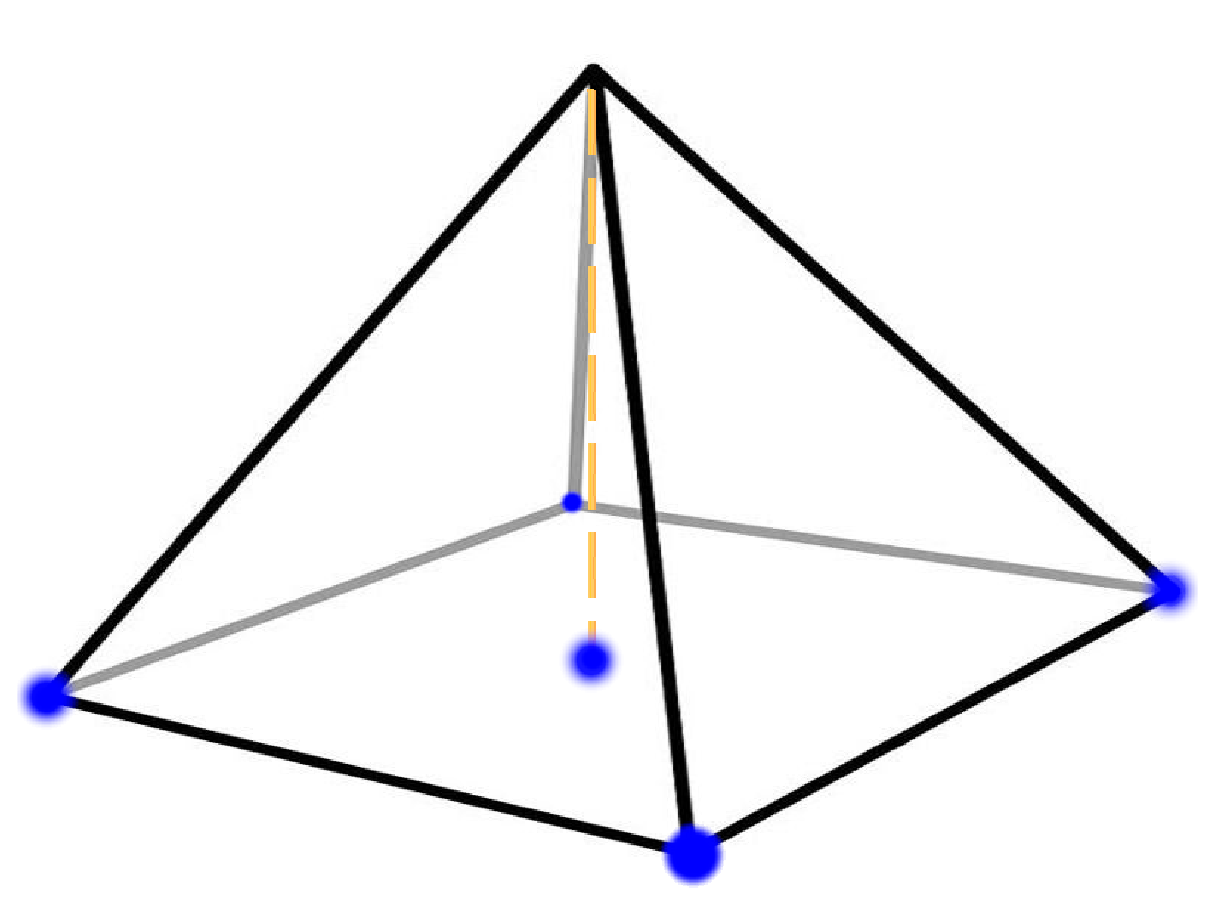
\includegraphics[width=0.5\linewidth]{figuras/piramide.eps}\\
  \caption{
Función de forma piramidal utilizada para producir las variaciones 
en el coeficiente de absorción. Esta función vale uno en el punto $\x_{\ell_1,\ell_2}$ 
y se anula a partir de los primeros vecinos de la grilla discreta.}
 \label{fig:priamid}
\end{figure}
 La función piramidal discretizada es aproximada como un producto 
 de deltas de Kronecker $\delta a_{\ell_1,\ell_2}=\delta_{r,\ell_1}\times\delta_{s,\ell_2}$.
 Llamando $\nabla_a g(\x_{\ell_1,\ell_2})$ al valor del gradiente funcional 
 en la dirección $\delta a_{\ell_1,\ell_2}$, la versión discreta 
 de la ecuación~\eqref{gradient_fin} resulta
\begin{equation}
\nabla_a g(\x_{\ell_1,\ell_2})  \sim -\sum_{m,j}  \lambda_{\ell_1,\ell_2,m,j}u_{\ell_1,\ell_2,m,j} \Delta \theta \Delta x \Delta y \Delta t,
\label{eq:FDwin22}
\end{equation}
donde $\lambda_{\ell_1,\ell_2,m,j}\sim
\lambda(\x_{\ell_1,\ell_2},\theta_m,t_j)$ y 
$u_{\ell_1,\ell_2,m,j} \sim u(\x_{\ell_1,\ell_2},\theta_m,t_j)$. 
Cabe notar que la ecuación~\eqref{eq:FDwin22} representa 
la derivada funcional para una única dirección $\delta a_{\ell_1,\ell_2}$ 
correspondiente a la componente $(\ell_1,\ell_2)$ del gradiente funcional discreto, 
donde el gradiente total discretizado estará dado por las perturbaciones en todas las direcciones posibles
\begin{equation}
\nabla_a g(\x)  = \left( \nabla_a g(\x_{1,1}), \nabla_a g(\x_{1,2}), \ldots, \nabla_a g(\x_{N_x+1,N_y+1})   \right).
\label{eq:grad_total}
\end{equation}
En el método adjunto, la evaluación de la ecuación~\eqref{eq:FDwin22} 
para todas las componentes $(\ell_1,\ell_2)$ del gradiente funcional requiere 
únicamente la resolución de un problema directo de transporte, y de 
su correspondiente problema adjunto para cada función generalizada $q=q_i$. 
En cambio, el uso de la ecuación~\eqref{eq:ObjFD} demanda la resolución de 
un número mucho más grande de problemas directos, donde debe evaluarse 
la resolución de $(N_x+1)\times (N_y+1)$ problemas de transporte, uno 
para cada perturbación del coeficiente $a(\x)$ en el dominio discretizado. 
Cabe mencionar también que el método adjunto requiere el almacenamiento 
en memoria de las soluciones completas a los problemas directos y adjunto de transporte 
para varios pasos temporales para realizar las integrales correspondientes~\eqref{eq:FDwin22}. 
El algoritmo paralelo propuesto en esta tesis es apropiado para este problema, ya que permite 
dividir simultáneamente el costo computacional y los requerimientos de memoria 
en sistemas distribuidos.
 
Como ilustración, en la figura~\ref{fig:gradient} se muestra 
el gradiente completo $\nabla_a g(\x_{\ell_1,\ell_2})$ para 
$1\leq \ell_1\leq N_x+1$ y $1\leq \ell_2\leq N_y+1$ 
para ciertos valores $\tilde G_{j,i}$, con una única fuente y 
un único detector ubicados en $\x_s=(1.5,0)$ y $\x_d=(1.0,0)$, 
respectivamente.

\begin{figure}[h!]
\centering
  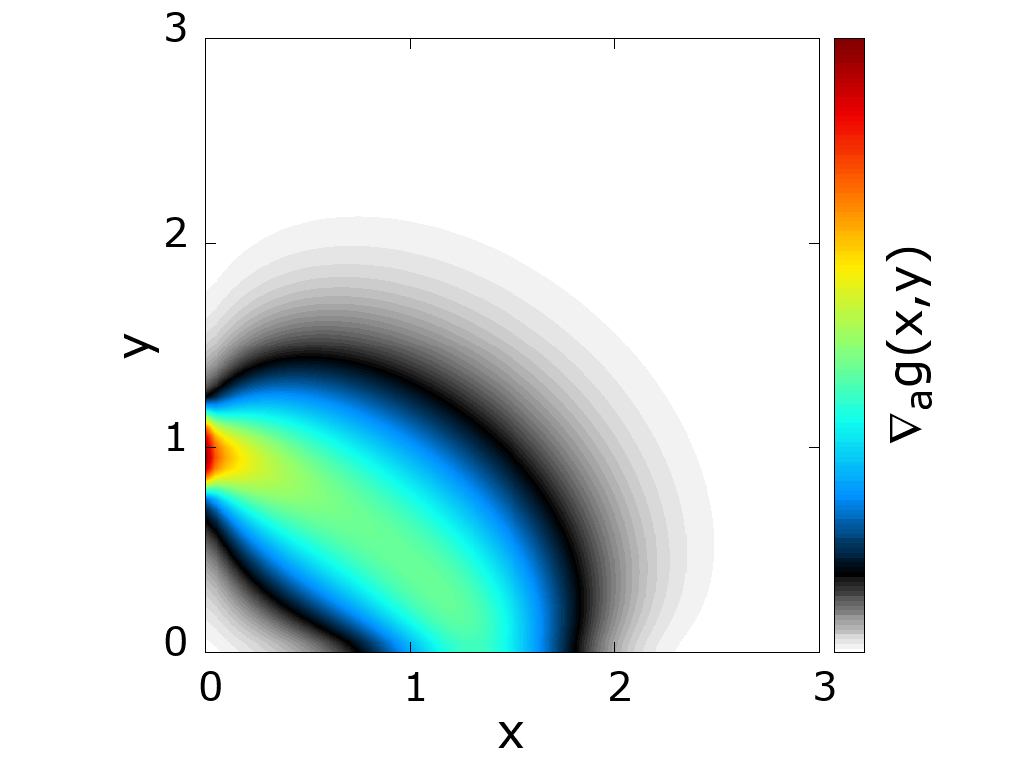
\includegraphics[width=0.5\linewidth]{figuras/gradient.png}
  \caption{
  Gradiente espacial~\eqref{eq:FDwin22} para todas 
  las direcciones discretas posibles $1\leq \ell_1\leq N_x+1$ y $1\leq \ell_2\leq N_y+1$, 
  con una única fuente y un único detector ubicados en $\x_s=(1.5,0)$ 
  y $\x_d=(0,1.0)$ respectivamente. Dado que se utilizaron 
  datos artificiales, la escala carece de sentido en esta figura, 
  y por eso no se muestra.}
 \label{fig:gradient}
\end{figure} 
 
\section{Datos sintéticos con fuentes láser pulsadas} 
\label{sec:sintetic} 

En las situaciones realistas en tomografía óptica, tipicamente 
radiación colimada proveniente de una fuente láser incide en 
la superficie del dominio en estudio. En esta sección damos 
algunos detalles para el modelo directo utilizado  
en las siguientes secciones para la resolución del problema inverso. 
Modelamos la radiación colimada de las fuentes láser por medio 
de una función picuda de la variable $\theta$, donde el pico 
de esta función coincide con la dirección del láser incidente. 
Resolvemos la ecuación~ \eqref{eq:RTE} con condiciones de Fresnel, 
utilizando los parámetros $a(\x)=0.1$/cm, $b(\x)=20$/cm, $g=0.8$, 
$n_{\Omega}=1.4$ y $n_s=1.0$, en un dominio espacial $\Omega=[x_{\text{min}},x_{\text{max}}]\times[y_{\text{min}},y_{\text{max}}]=[0,3]\times[0,3]$. 

Mostraremos resultados para el método MB, y el método FMS. 
En el método MB empleamos una única fuente generalizada~\eqref{eq:RTEsources}, 
con $N_q=N_s=1$, centrada en $\x_{1,1}=(1.5,0)$, apuntando en la dirección 
normal a la superficie, de forma qué $\theta_{1,1}=\pi/2$, con $\sigma_{\theta}=\pi/4$. 
En esta configuración, una fuente láser inyecta radiación $y_{\text{min}}$ en la dirección 
normal a $\partial \Omega$ (Fig.~\ref{fig:photonflux}).
\begin{figure*}[h!]
\centering
  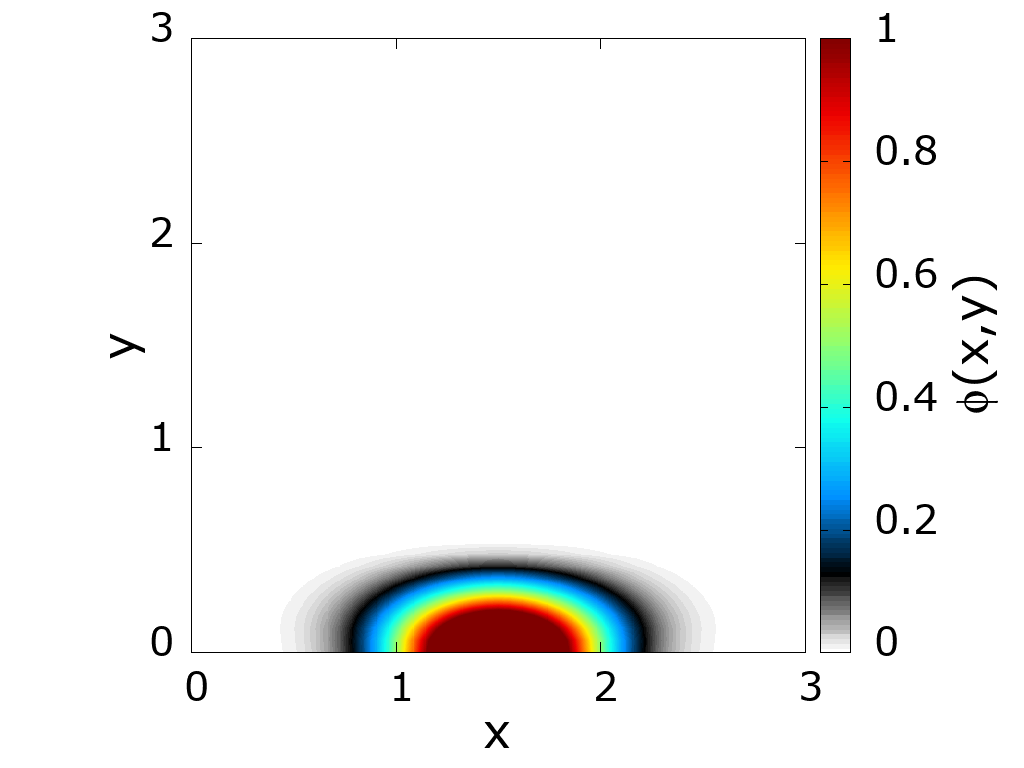
\includegraphics[width=0.325\textwidth]{figuras/sim_MB_t30.png}
  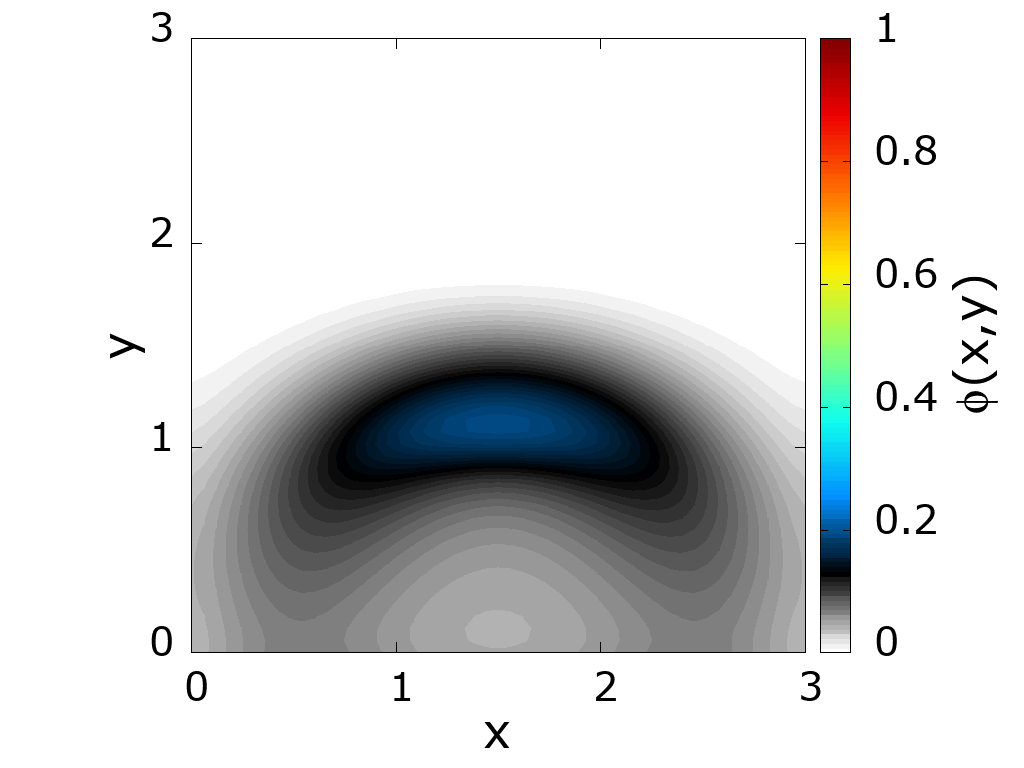
\includegraphics[width=0.325\textwidth]{figuras/sim_MB_t100.png}
  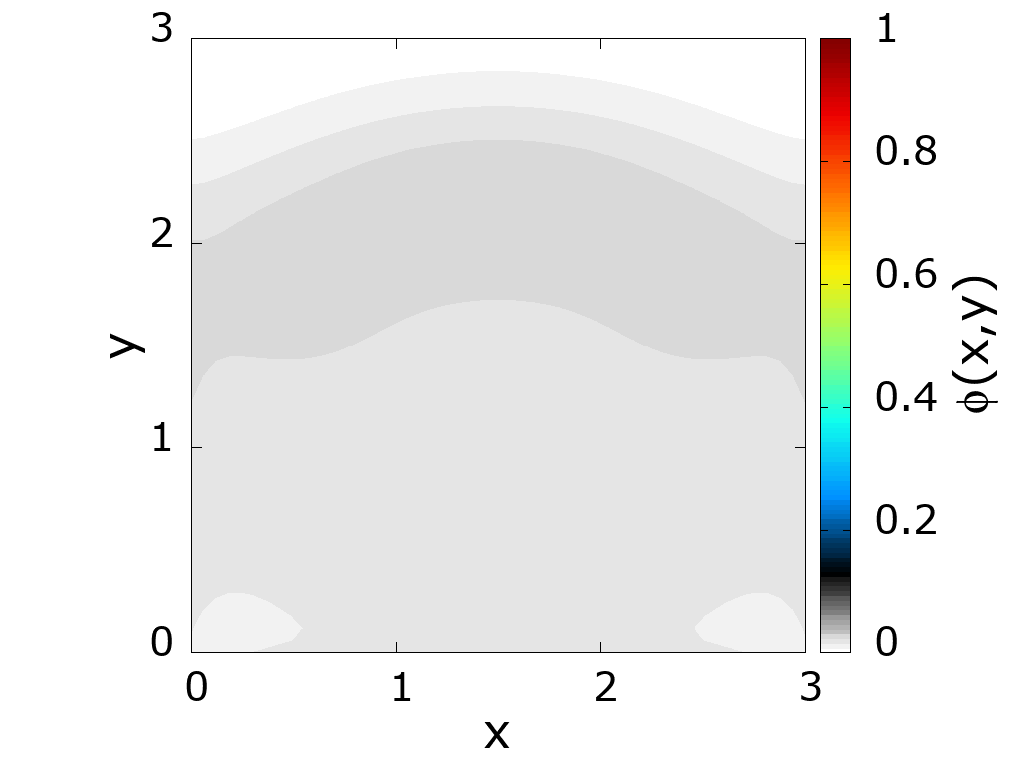
\includegraphics[width=0.325\textwidth]{figuras/sim_MB_t170.png}
  \caption{Simulación para el modelo directo MB utilizando 
  el método FC--DOM en paralelo~\ref{algfc} presentado en 
  la sección~\ref{subsec:FC-DOM}. En la figura se muestra el 
  flujo escalar $\phi(\x,t)$, ec.~\eqref{eq:photondensity} para tres tiempos 
  diferentes utilizando el método MB con una única fuente generalizada. De 
  izquierda a derecha se tiene $t=30$ps, 
$t=100$ps y $t=170$ps, para una fuente láser 
inyectando radiación en  $\x_s=(1.5,0)$cm. La figura muestra la evolución 
temporal de una ``onda de flujo de fotones'' difusos.}
 \label{fig:photonflux}
\end{figure*}
 
Para el método FMS, utilizamos una única fuente generalizada, con cuatro 
fuentes superpuestas, de forma qué $N_q=1$ y $N_s=4$. Cada fuente inyecta 
radiación en la dirección normal a $\partial \Omega$ a través del 
centro de las caras, con retardos temporales $\tau=200$ps entre fuentes sucesivas, 
comenzando con la fuente ubicada en $y_{\text{min}}$, seguida de la fuente 
en $y_{\text{max}}$, luego la ubicada en $x_{\text{min}}$ y finalmente 
se enciende la fuente en $y_{\text{max}}$ (Fig.~\ref{fig:photonflux2}).   
 

\begin{figure*}[h!]
\centering
  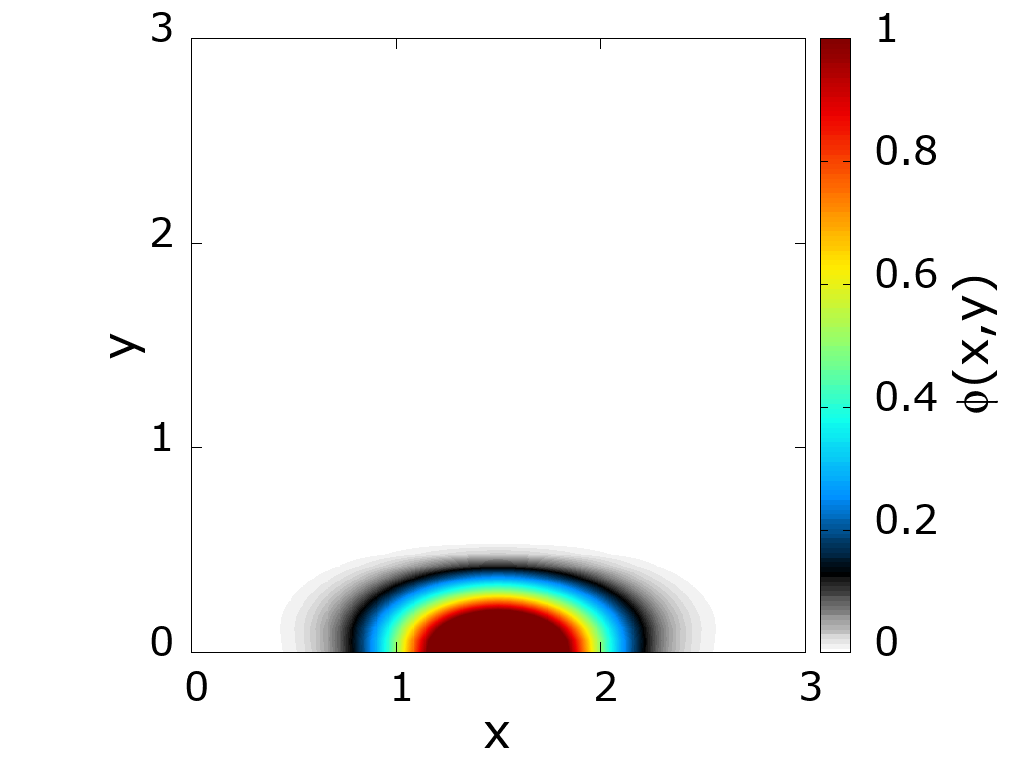
\includegraphics[width=0.325\textwidth]{figuras/sim_FMS_t30.png}
  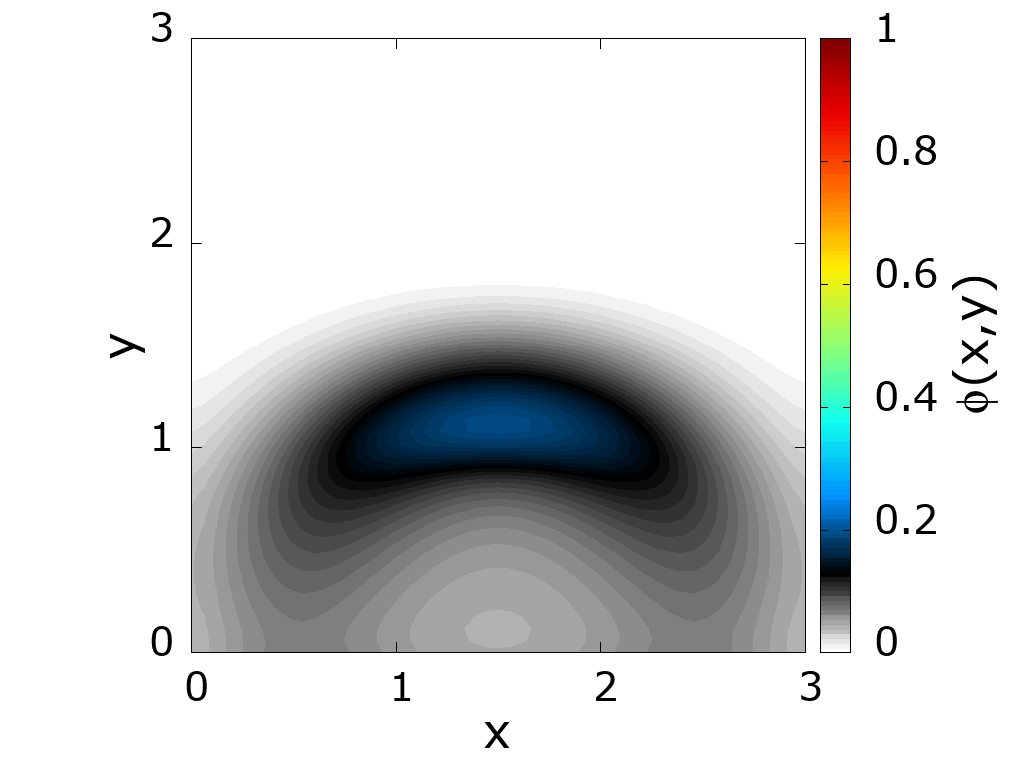
\includegraphics[width=0.325\textwidth]{figuras/sim_FMS_t100.png}
  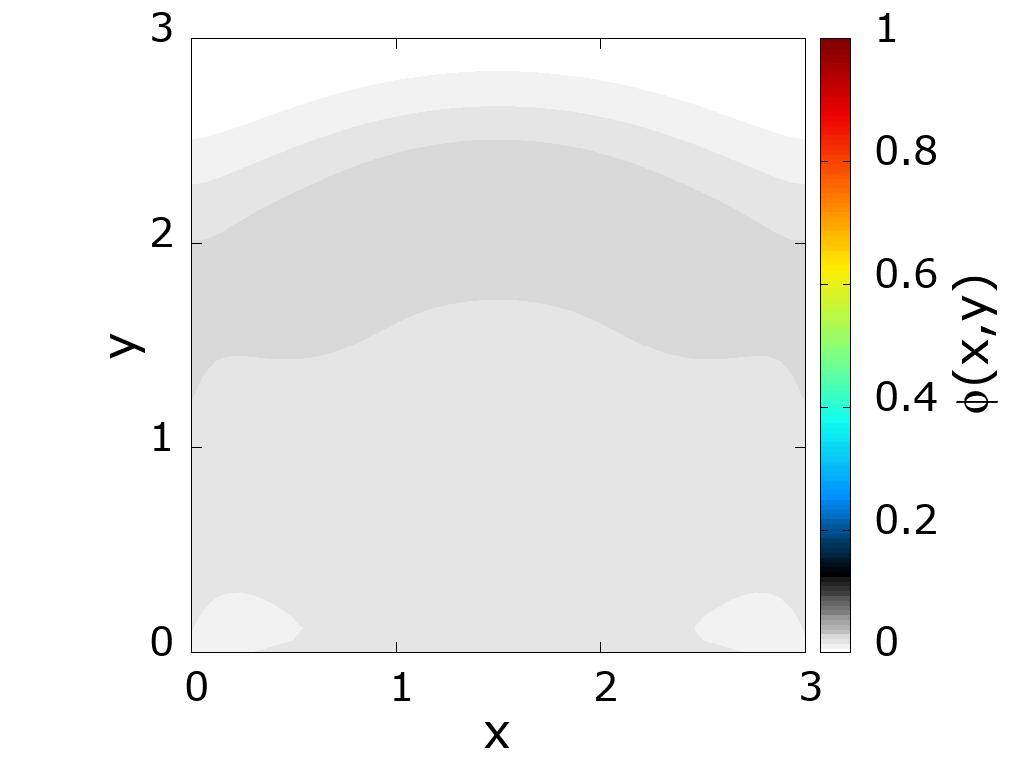
\includegraphics[width=0.325\textwidth]{figuras/sim_FMS_t170.png}\\
  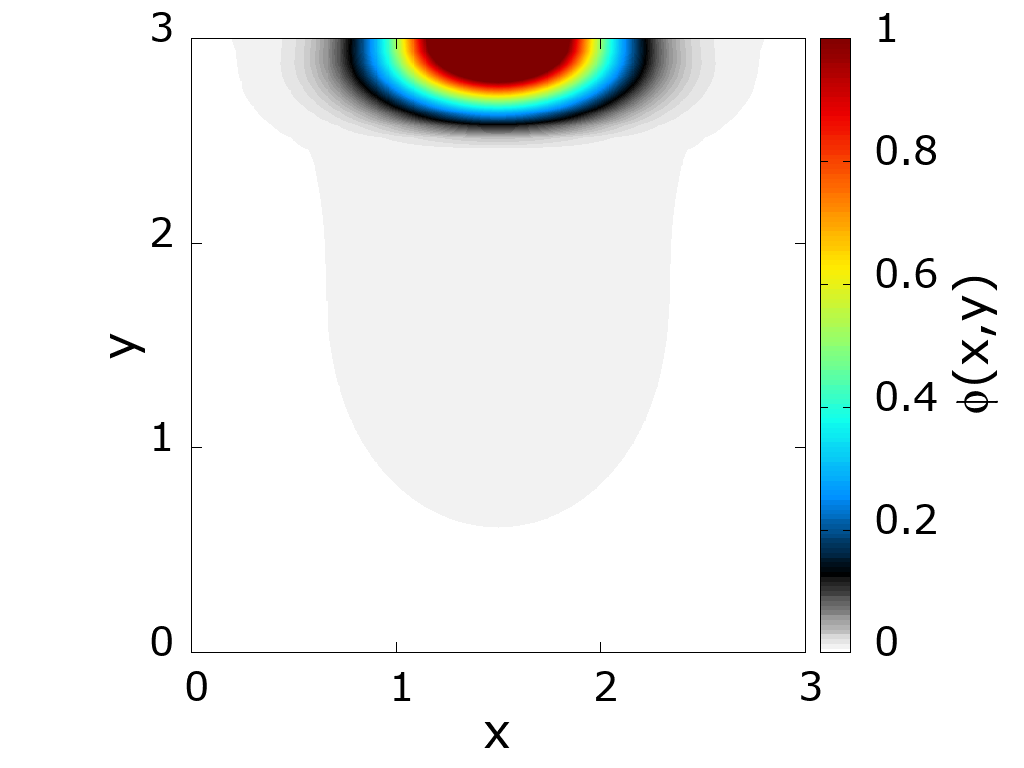
\includegraphics[width=0.325\textwidth]{figuras/sim_FMS_t230.png}
  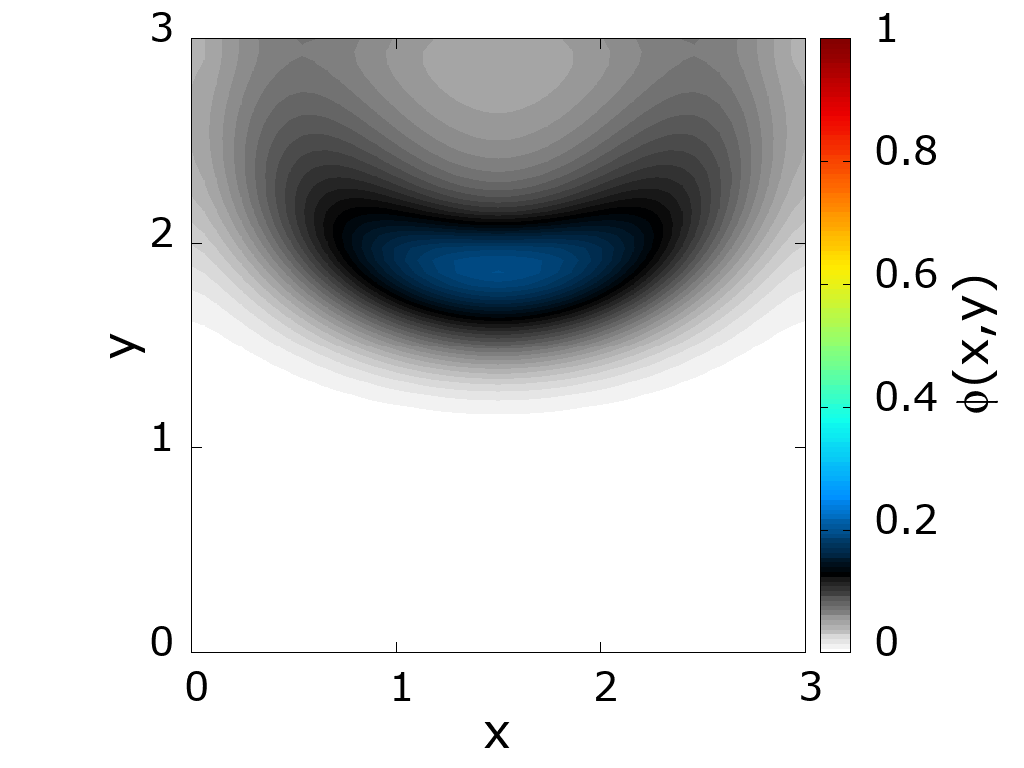
\includegraphics[width=0.325\textwidth]{figuras/sim_FMS_t300.png}
  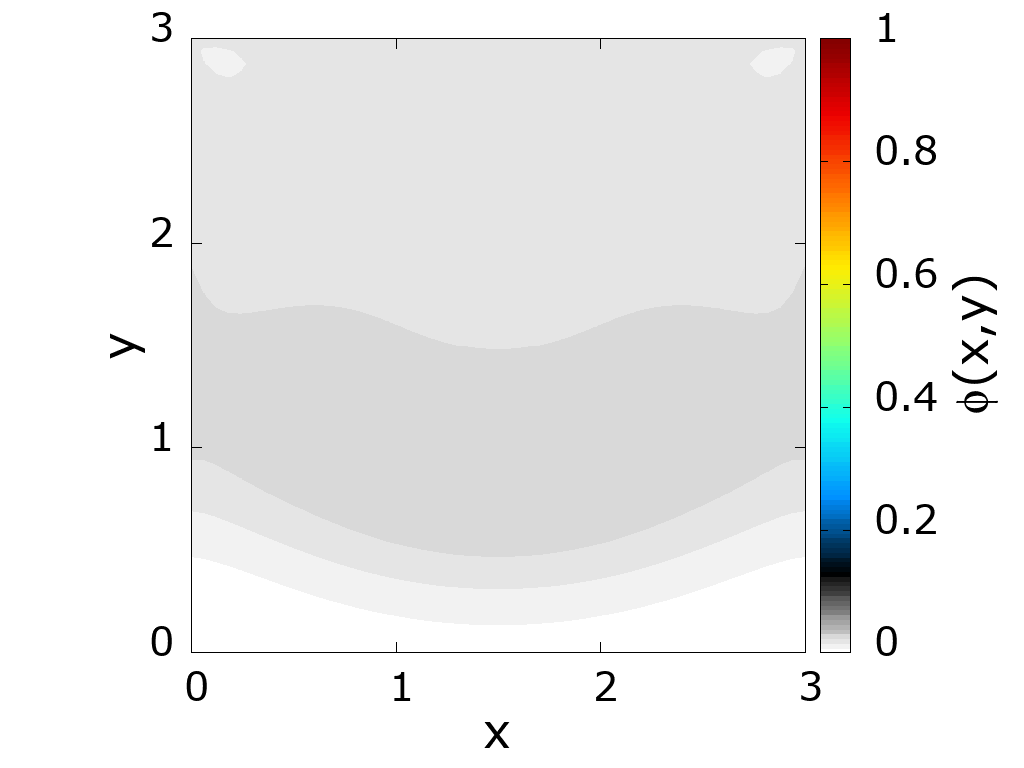
\includegraphics[width=0.325\textwidth]{figuras/sim_FMS_t370.png}\\
  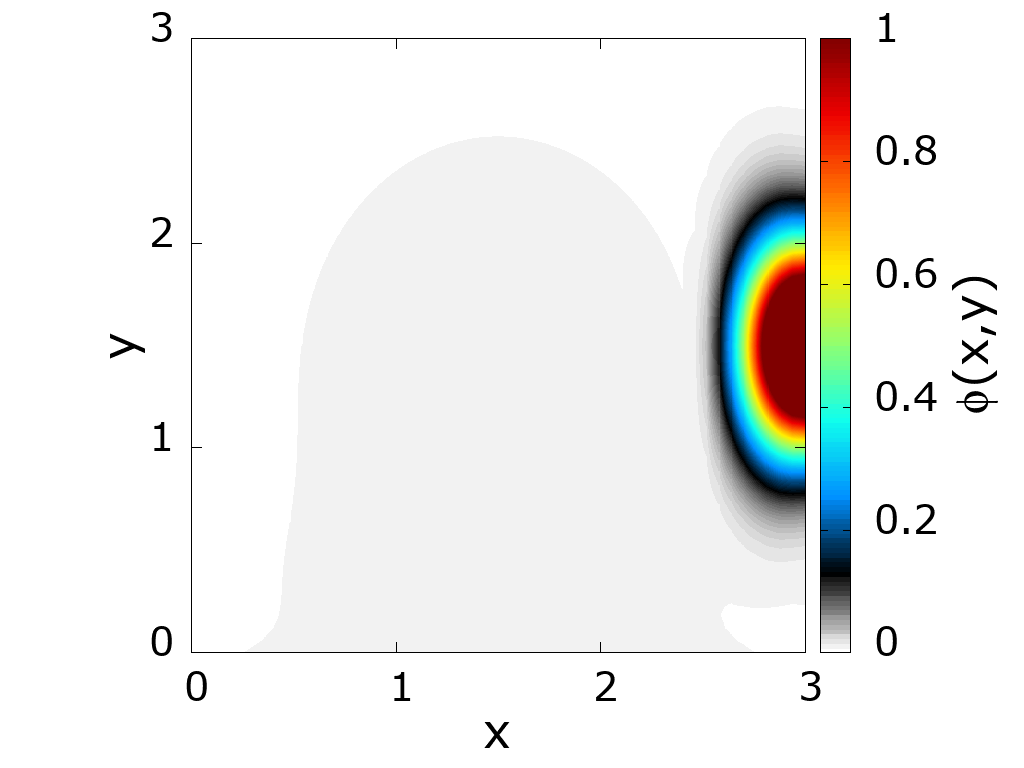
\includegraphics[width=0.325\textwidth]{figuras/sim_FMS_t430.png}
  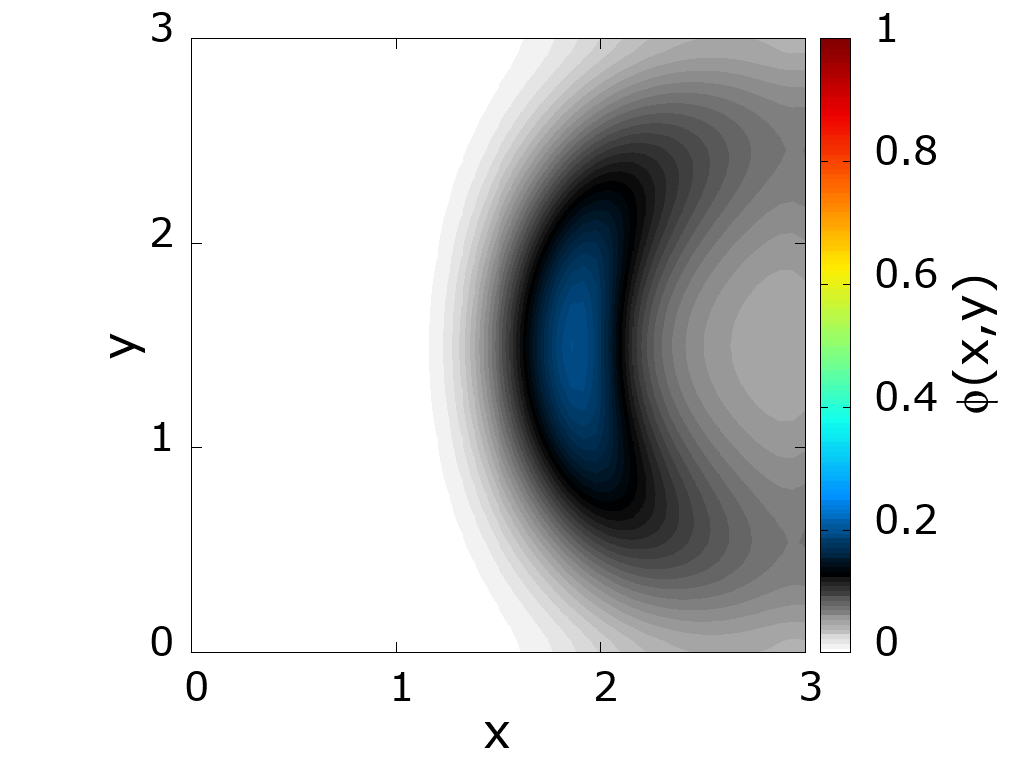
\includegraphics[width=0.325\textwidth]{figuras/sim_FMS_t500.png}
  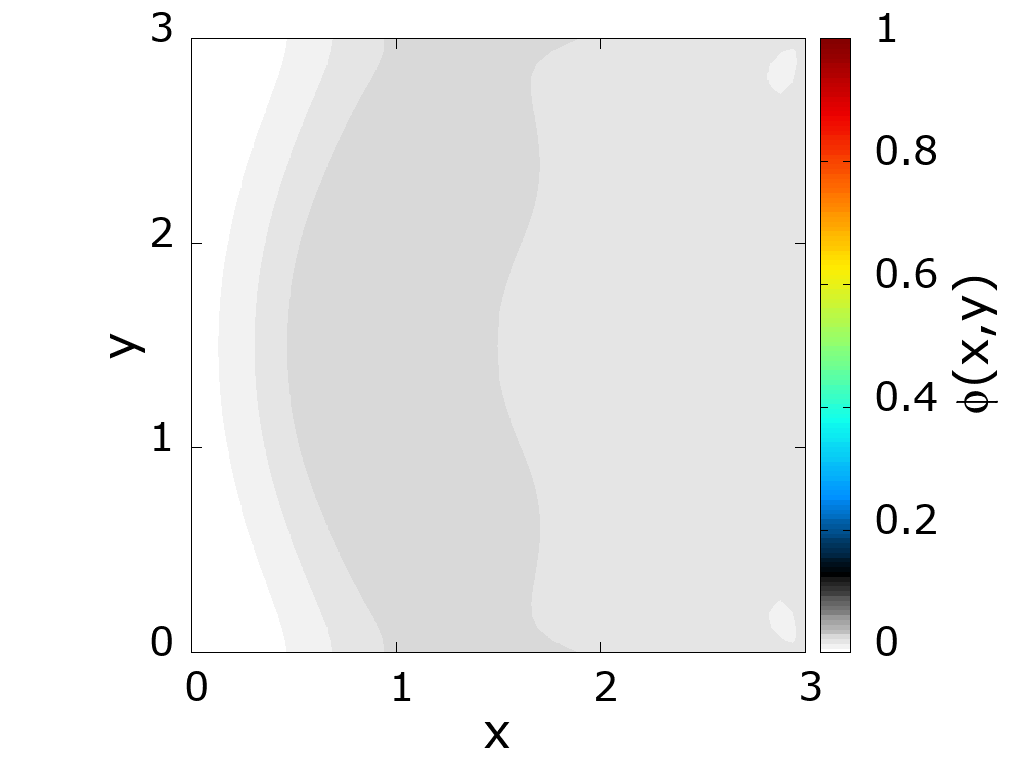
\includegraphics[width=0.325\textwidth]{figuras/sim_FMS_t570.png}\\
  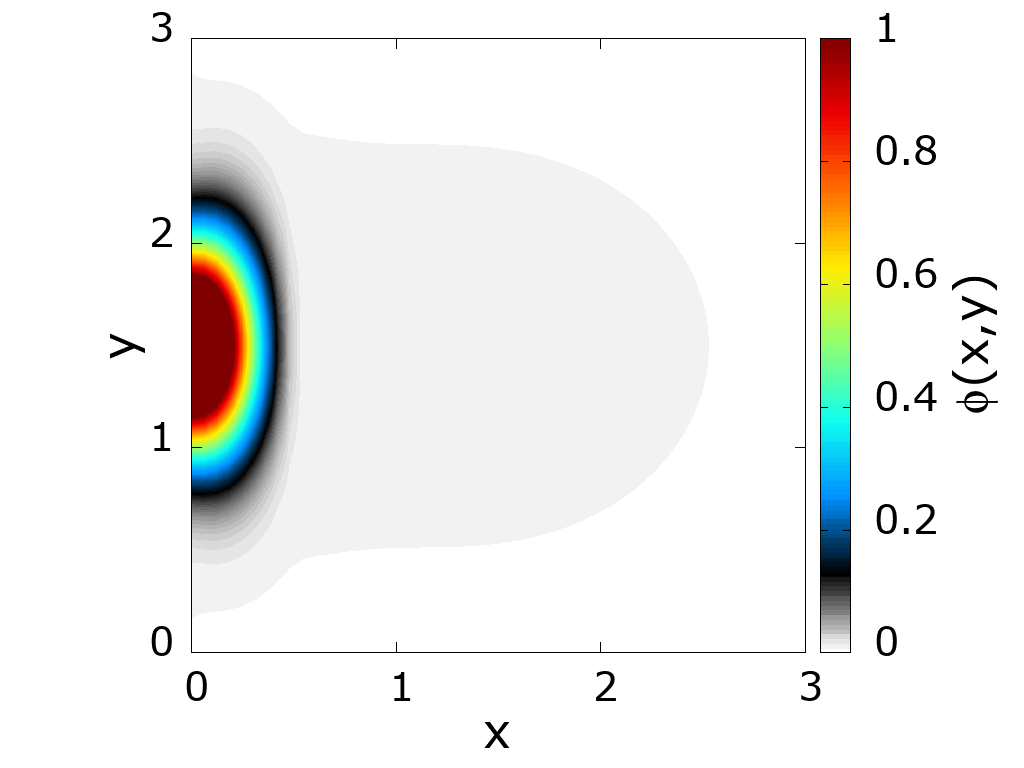
\includegraphics[width=0.325\textwidth]{figuras/sim_FMS_t630.png}
  \includegraphics[width=0.325\textwidth]{figuras/sim_FMS_t700.png}
  \includegraphics[width=0.325\textwidth]{figuras/sim_FMS_t770.png}
  \caption{Simulación para el modelo directo FMS utilizando 
  el método FC--DOM en paralelo~\ref{algfc} presentado en 
  la sección~\ref{subsec:FC-DOM}. En la figura se muestra el 
  flujo escalar $\phi(\x,t)=\phi(\x)$, ec.~\eqref{eq:photondensity} para tiempos 
  diferentes utilizando el método FMS con una única fuente generalizada 
  que contiene cuatro fuentes láser superpuestas, con tiempos de retraso $\tau=200$ps. De 
  izquierda a derecha y de arriba hacía abajo, se tiene $t=30$ps, $t=100$ps y $t=170$ps, 
   $t=230$ps, $t=300$ps y $t=370$ps,  $t=430$ps, $t=500$ps y $t=570$ps, 
    $t=630$ps, $t=700$ps y $t=770$ps.}
 \label{fig:photonflux2}
\end{figure*}

Para las reconstrucciones numéricas presentadas en la sección siguiente, utilizamos 
datos ``sintéticos'', esto es, datos generados de manera numérica 
con el algoritmo FC--DOM, para un dado 
coeficiente $a(\x)$. Dado que en situaciones realistas se espera 
que los datos experimentales presenten ruido, agregamos a los 
datos sintéticos un 10\% de ruido aleatorio a los datos sintéticos simulados 
utilizados en las reconstrucciones del problema inverso. 


Como puede observarse en la figura~\ref{fig:photonflux2}, para el método 
MB, dado que cada fuente láser individual es tratada mediante una simulación 
independiente de las otras fuentes, cada señal originada por los fotones 
transportados en el medio participante desde el láser hasta los detectores 
se encuentra desacoplada de la señal de las otras fuentes. En el método 
FMS, en cambio, las señales de todas las fuentes láser individuales 
aparece mezclada en los detectores.  El rol de los retardos temporales 
utilizados en el método FMS es desacopla en algún grado para 
un dado detector las señales 
originadas por fuentes láser individuales proveniente desde diferentes lugares.  

\begin{figure}[h!]
\centering
  \includegraphics[width=0.48\linewidth]{figuras/detread_sweep.eps}
  \includegraphics[width=0.48\linewidth]{figuras/detread_prop.eps}
  \caption{Lectura del detector $G[u_1]$ en la ec.~\eqref{eq:OpMed} para 
  una única fuente generalizada del método MB, y una fuente generalizada con 
  $N_s=4$ para el métofo FMS, antes y después de agregar un 10\% de ruido aleatorio 
  a la señal. El detector utilizado se ubicó en  $\x_d=(3.0,2.25)$. Cada fuente 
  láser individual se ubicó en el centro de las caras del dominio cuadrado. 
  Como puede observarse, en el método FMS las lecturas de los detectores 
  aparecen mezcladas. Utilizamos un retraso temporal  $\tau=200$ps entre las fuentes 
  ubicadas en las diferentes caras.}
 \label{fig:detread}
\end{figure}

\section{Algoritmo para la resolución del problema inverso}
\label{sec:inversesolv}

Como se indico anteriorment, el algoritmo propuesto en esta tesis para la resolución del 
problema inverso incorpora, en particular, la estrategia FMS, basada 
en el uso de fuentes que se aplican en un único problema directo, 
en lugar de la estrategia MB utilizada previamente en la literatura. 
En el método MB, por cada fuente láser deben realizarse un par 
de simulaciones para el problema dirécto y el problema adjunto, 
para luego combinar los resultados para obtener el gradiente utilizado 
en el método lm-BFGS. En cambio, en el método FMS propuesto, 
se construye la función objetivo utilizado una única fuente 
generalizada que contiene a todas las fuentes láser, de forma tal 
que se utiliza un único par de simulaciones para los problemas directos 
y adjuntos, lo cual, como se demuestra en la sección~\ref{sec:inverseres} 
(de manera cualitativa en las figuras~\ref{fig:itdet} y~\ref{fig:ithead} 
y de forma cuantitativa en las figuras~\ref{fig:reconst} y~\ref{fig:rechead}) 
reduce los tiempos de computo para el problema inverso de manera significativa 
(\eg en un factor de seis en la figura~\ref{fig:ithead}), sin que se 
produzca un deterioro en la calidad de la imagen obtenida. 

Buscamos el coeficiente de absorción que minimiza la ec.~\eqref{eq:FObjpr}  
sujeto a las restricciones $a^l(\x) \leq a(\x) \leq a^u(\x) \forall \x$, \ie, buscamos 
el coeficiente $a(\x)$ que es solución del problema 
\begin{equation}
\begin{split}
\begin{aligned}
a(\x)=\text{argmin}_{a^l \leq \widetilde a(\x) \leq a^u} \Lambda[a]
\end{aligned}
\end{split}
\label{eq:minprob}
\end{equation}

Las restricciones impuestas en el proceso de minimización estan dadas 
por propiedades generales conocidas del coeficiente de absorción ($a^l(\x)\ge 0$ 
es una condición física que siempre debe cumplirse), y por cierto conocimiento 
del coeficiente, obtenido previamente por otras técnicas tomográficas, lo 
cual reduce el espacio de soluciones admisibles al problema de minimización~\eqref{eq:minprob}.

El algoritmo para la resolución del problema inverso~\ref{algfcinv},
procede de la siguiente manera. A partir de una estimación inicial $a^0(\x)$ para el
coeficiente de absorción y utilizando las lecturas de los detectores experimentales
$\widetilde{G}_{j,i}$, con $j=1, \ldots,N_d$ y $i=1,\ldots,N_q$, se resuelven
los problemas directos y adjuntos~\eqref{eq:RTE}
y~\eqref{eq:AdjointProblem}, a partir de lo cual se calcula el gradiente 
funcional~\eqref{eq:FDwin22}. El gradiente funcional 
se pasa al algoritmo lm-BFGS, que devuelve una actualización para 
coeficiente de absorción $a^1(\x)$ que reduce las diferencias entre
las lecturas de los detectores experimentales y los valores para los detectores simulados.
La iteración de este procedimiento converge, mediánte el método lm-BFGS, al mínimo 
de la función objetivo~\eqref{eq:FObjpr}.

El algoritmo para la solución del problema inverso de transporte radiativo, 
para un dado número de iteraciones $i_{\text{max}}$, se sumariza en el 
algorítmo~\ref{algfcinv}. En este algoritmo, $C \in \mathbb{R}$ representa un criterio 
de convergencia preestablecido. El algorítmo se itera mientras el valor 
de la función objetivo esté por encima de dicho criterio de convergencia.
\begin{algorithm}
\caption{Algoritmo para la resolución del problema inverso en paralelo}
\label{algfcinv}
\begin{algorithmic}[1]
\State Dar una estimación inicial $a^0(\x)$
\State \textbf{para} $i=1,\ldots,i_{\text{max}}$ \textbf{hacer}
\State \hskip0.5em \textbf{para} cada fuente generalizada $q_j, j = 1,\ldots,N_q$ \textbf{hacer}
\State \hskip0.75em Resolver el problema directo por medio del algoritmo~\ref{algfc}
\State \hskip0.75em Evaluar ec.~\eqref{eq:FObjpr}, sí $ \Lambda[a] < C $ ir a \ref{al:end}.
\State \hskip0.75em Resolver el problema adjunto mediante el algoritmo~\ref{algfc}
\State \hskip0.5em\textbf{terminar}
\State \hskip0.5em Construir el gradiente ec.~\eqref{eq:FDwin22}
\State \hskip0.5em Llamar al algoritmo lm-BFGS para actualizar el coeficiente $a^{i+1}(\x)$.       
\State \label{al:end} \textbf{terminar} con $a(\x)=a^i(\x)$
\end{algorithmic}
\end{algorithm}


\section{Reconstrucciones numéricas}
\label{sec:inverseres}
En esta sección aplicamos los algoritmos desarrollados 
en las secciones previas al problema inverso en tomografía óptica. 
Los problemas inversos en tomografía óptica que consideramos 
conciernen a configuraciones en las cuales se buscan inclusiones 
sobre un tejido de ``fondo'' que se asume conocido. Esta situación describe, 
\eg, los excesos en la absorción de la radiación originados 
por la presencia de hemoglobina oxígenada en el cerebro, 
producida por la respuesta hemodinámica debido a la activación 
de una región determinada del cerebro~\cite{Boas2001,bluestone2001,Arridge1999,Hernandez2020}, 
para aplicaciones neurocientíficas, 
o el exceso de hemoglobina oxigenada originada por la presencia de un tumor 
para aplicaciones en diagnósticos médicos~\cite{Althobaiti2017,Guven2003,Zhu2005,Zhu2010,Fujii2016b}.

La primera demostración que haremos ilustrará una aplicación potencial 
de la técnica de tomografía óptica para el diagnóstico 
de un paciente para el cual se dispone de una imágen por resonancia magnética (MRI)
del cuello (fig.~\ref{fig:mriim}). Describimos una situación teniendo 
en mente la aplicación potencial para el estudio de la evolución de la metástasis 
en una región específica del cuerpo (el cuello), tiempo después 
de haber adquirido la imagen MRI. Similarmente, el procedimiento 
podría utilizarse para seguir la evolución del tratamiento de un tumor en esta región. 
La portabilidad y el bajo costo de los sistema de tomografía óptica 
hace que estos dispositivos sean mucho mas accesibles para el diagnóstico 
que las imágenes obtenidas por sistemas MRI, para monitorear 
la evolución del tratamiento y el avance de un tumor de forma regular. 

En las referencias~\cite{Fujii2016b,Fujii2016} se realizó un estudio sobre el problema directo de la propagación de la luz en el cuello humano. Aquí presentamos un modelo similar,
 y extendemos la idea para el estudio 
de la convergencia del problema inverso siguiendo las lineas de las referencias~\cite{Fujii2016b,Fujii2016} con la intención de capturar 
algunas de las características mas importantes del cuello humano, 
manteniendo una geometría simple. 

Estudiaremos la convergencia por iteración del algoritmo~\ref{algfcinv} 
para un número variable de fuentes y detectores, para una dada configuración. 
Para evaluar la convergencia en el proceso de reconstrucción cuantificamos 
el error en la norma $L^2$ definido como
\begin{equation}
\begin{split}
\begin{aligned}
E(i)=\sqrt{\frac{\int_{\Omega}(a^v(\x)-a^i(\x))^2  d\x}{\int_{\Omega}a^v(\x) d\x}}
\end{aligned}
\end{split}
\label{eq:errl2}
\end{equation}
donde $E(i)$ corresponde al error en la norma $L^2$ para la iteración $i$, 
donde $a^v(\x)$ es el coeficiente de absorción ``verdadero'', y $a^i(\x)$ 
es el coeficiente de absorción obtenido por el algorítmo~\ref{algfcinv} 
en la iteración $i$-ésima. 

Buscaremos la existencia de un tumor en el tejido blando. 
Los coeficientes de la columna vertebral, la médula espinal, y la tráquea 
se mantendrán fijos en el proceso de reconstrucción, con $a^l(\x)=a^u(\x)=a(\x)$ 
en estas regiones, con los coeficientes dados para cada tipo de tejido correspondiente, 
los cuales se presentan en la tabla~\ref{tab:cuello}, y fueron tomados de las referencias~\cite{Bashkatov2011,Dehaes2011,Fujii2016}.

\begin{table}[h!]
\caption{Propiedades ópticas para el modelo de cuello humano}
\vspace{-0.3cm}
\begin{center}
\begin{tabular}{ccccccc}
\hline
Órgano & ~ $a[1/cm]$ & ~ & $b[1/cm]$ ~ & $g$ ~ & $n_{\Omega}$ \\
\hline
Tejido blando & ~$0.3$ & ~ & $80$ ~ &$0.9$ ~  & $1.4$ \\
Tráquea & ~$0.0$ & ~ & $0.0$ ~ &$0.0$ ~ &  $1.0$\\
Columna vertebral & ~$0.25$ & ~ & $148$ ~ &$0.9$   ~ &  $1.4$ \\
Médula espinal & ~$0.17$ & ~ & $882$ ~ &$0.9$  ~ &  $1.4$ \\
\hline
\end{tabular}
\label{tab:cuello}
\end{center}
\end{table}
Para simplificar el modelo, tomamos el coeficiente de refraxión 
de la traquea cómo $n_{\Omega}=1.4$. Esto evita las dificultades 
encontradas para el modelado de la interfase entre la traquea y el tejido blando, 
el cual para un modelado mas preciso requiere tener en cuenta la reflexión 
de Fresnel en esta interfase goemétricamente compleja. Otras simplificaciones 
adicionales utilizadas consistieron en no considerar los vasos sanguíneos, y en la 
simplificación de la geometría del cuello, el cual se tomo como una geometría 
cuadrada.

Por otra parte, fijamos el valor  $a(\x)=a^l(\x)=a^u(\x)$ 
al valor del fondo en las proximidades de los bordes, para puntos 
a una distancia menor a $0.5$cm. Este procedimiento genera una mejor 
convergencia en el problema de reconstrucción del coeficiente $a(\x)$, y previene 
la amplificación de los errores numéricos, originados por la existencia 
de las capa límite~\cite{Gaggioli2021} discutidas en la sección~\ref{sec:blayer}. 
La resolución de la capa límite en el problema multidimensional exige de métodos 
numéricos más sofisticados que escapan al alcance de esta tesis. 

Aplicamos el algoritmo para la reconstrucción del coeficiente 
de absorción, y comparamos los métodos MB y FMS propuesto en este trabajo. 
Para ello, producimos datos sintéticos de la forma descripta en la sección~
\ref{sec:sintetic}, donde agregamos un 10\% de ruido aleatorio a los datos obtenidos 
para los detectores mediante las simulaciones numéricas, de forma de obtener 
resultados que se acerquen a una situación experimental real.

Como mencionamos anteriormente, la situación que simulamos es una en la cual se buscan inclusiones sobre 
cierto ``fondo'' conocido. La situación que ilustramos en este primer caso corresponde 
a los excesos de absorción 
originados por la presencia de hemoglobina oxigenada debido a la presencia de un tumor 
en el tejido, lo cual encuentra aplicaciones tanto en el diagnostico de la enfermedad, así 
como en el seguimiento del tratamiento de la misma.

El mínimo $a^l$ para el coeficiente de absorción vendrá dado 
por los valores del ``fondo'' del tejido analisado (que se asume conocido \textit{a priori}). 
El límite superior estará dado por valores típicos del coeficiente de absorción 
para el tejido que se está examinando, y lo fijaremos en $a^u=1$.

La imagen MRI es tomada como el coeficiente inicial $a^0(\x)$
para la iniciación de las iteraciones. 

\begin{figure}[h!]
\centering
  \includegraphics[width=0.25\linewidth]{figuras/neck_mri.png} 
  \caption{Imagen de Resonancia Magnética~\cite{CCommons} para el modelo de cuello humano empleado. } 
 \label{fig:mriim}
\end{figure}

\begin{figure}[h!]
\centering
  \includegraphics[width=0.48\linewidth]{figuras/neck_i.png} 
  \includegraphics[width=0.48\linewidth]{figuras/neckmss_scatt.png} 
  \caption{Izquierda: coeficiente de absorción 
  generado a partir de la imagen~\ref{fig:mriim}, el cual fue utilizado como el coeficiente 
  inicial $a^0(\x)$ en las reconstrucciones del coeficiente de absorción para éste modelo. 
  Derecha: coeficiente de dispersión para el modelo de cuello humano.
  Los coeficientes de absorción y dispersión 
  para los distintos órganos fueron tomados de las referencias\cite{Bashkatov2011,Dehaes2011,Fujii2016}. } 
 \label{fig:mriimc}
\end{figure}

En esta demostración, para el método FMS empleamos una única fuente generalizada 
la cual contiene multiples fuentes láser. Las diferentes fuentes láser 
contenidas en esta única fuente generalizada iluminan el borde del dominio $\partial \Omega$ 
en la dirección normal al mismo, inyectando la radiación que atraviesa 
el medio participante, sensándolo, y luego es recolectada por los detectores. 
La configuración que elegimos para la activación de las fuentes es tal 
que se activan de manera simultánea una fuente por cara. 
Utilizamos un retraso temporal de $300$ps para fuentes vecinas ubicadas 
en una misma cara. En detalle, para el caso con 16 fuentes, fijamos 
$\tau_{1,1}=0$ps para las fuentes simultáneas ubicadas en $\x_1^1=(2.0,0.0)$, 
$\x_1^2=(10.0,2.0)$, $\x_1^3=(8.0,10.0)$,  $\x_1^4=(0.0,8.0)$, donde utilizamos 
el supraíndice para indicar las diferentes fuentes láser individuales, y el subíndice 
para indicar el teimpo de retraso temporal correspondiente $\tau_{k,1}$ (ver la ecuación~\eqref{eq:RTEsources}).
El resto de las fuentes se configuran de la siguiente manera: 
$\x_2^1=(4.0,0.0)$, 
$\x_2^2=(10.0,4.0)$, $\x_2^3=(6.0,10.0)$,  $\x_2^4=(0.0,6.0)$ con $\tau_{2,1}=300$ps, 
$\x_3^1=(6.0,0.0)$, 
$\x_3^2=(10.0,6.0)$, $\x_3^3=(4.0,10.0)$,  $\x_3^4=(0.0,4.0)$ con $\tau_{3,1}=600$ps 
and $\x_4^1=(4.0,0.0)$, 
$\x_4^2=(10.0,4.0)$, $\x_4^3=(6.0,10.0)$,  $\x_4^4=(0.0,6.0)$ con retraso temporal $\tau_{4,1}=900$ps. 

Este arreglo fue guiado por la idea de utilizar en el métofo FMS como fuentes simultaneas 
aquellas que están geométricamente más alejadas unas de otras. Debido 
al decaimiento exponencial en la onda de densidad de fotones difusos (ver fig.~\ref{fig:photonflux}), es esperable que cada fuente láser tenga un efecto despreciable en las lecturas de los detectores cercanos a otras fuentes geométricamente lejanas, 
aún cuando fueron activadas de manera simultánea. Para dar tiempo suficiente 
a la relajación de las ondas de fotones producidas por las fuentes activadas 
de forma más tardía, cada simulación directa en el método FMS fue evolucionada 
hasta el tiempo final $t_{\text{max}}=1400$ps. Para los casos en los que se utilizaron 
un número menor de fuentes, la configuración para la activación de las mismas 
fue similar. Para el método MB, cada simulación directa fue evolucionada hasta el tiempo 
final $t_{\text{max}}=600$ps, con los detectores y las fuentes ubicados en las mismas 
posiciones que las utilizadas en el método FMS, y utilizando las mismas grillas numéricas, 
e igual número de procesadores en cada caso.

\begin{figure*}[h!]
\centering
  \includegraphics[width=0.49\textwidth]{figuras/detsSweep.eps}
  \includegraphics[width=0.49\textwidth]{figuras/detsMSS.eps}
\\
    \vspace{0.3cm}
  \includegraphics[width=0.49\textwidth]{figuras/sourcesSweep.eps}
  \includegraphics[width=0.49\textwidth]{figuras/sourcesMSS.eps}
  \caption{Convergencia obtenida para el error en la norma $L^2$ ec.~\eqref{eq:errl2} 
  del coeficiente de absorción con respecto al número de iteraciones, 
  para un número variable de detectores (arriba) y de fuentes láser (abajo), para los métodos 
  MB y FMS. 
   A la izquierda: 
  error en la norma $L^2$ ec.~\eqref{eq:errl2} para 100 iteraciones del método MB. 
  Derecha:error en la norma $L^2$ ec.~\eqref{eq:errl2} para 100 iteraciones del método FMS. 
  Para las simulaciones en el panel superior se utilizaron 16 fuentes láser. Para 
  las simulaciones en el panel inferior, se utilizaron 36 detectores.}
 \label{fig:itdet}
\end{figure*}


Como puede apreciarse en la figura~\ref{fig:itdet}, los métodos MB y FMS 
presentan propiedades de convergencia similares para un número variable 
de fuentes y detectores. Sin embargo, para el caso con 16 fuentes, 
el método FMS tomó  $12689$ segundos para llegar a las 100 iteraciones, 
del algoritmo~\ref{algfcinv}, mientras que el método MB tomó $88093$ segundos, 
dando una aceleración en la reconstrucción por un factor cercano a siete. 
En la figura además se aprecia que incrementar el número de fuentes y de detectores 
genera una mejora considerable en la convergencia del problema inverso 
para un número fijo de iteraciones. El número de fuentes tiene un impacto 
mayor en las reconstrucciones que el número de detectores. 
Esto puede entenderse de la siguiente manera, dado que la función de las fuentes 
es producir los fotones que viajan a través del medio participante para sensarlo 
y finalmente ser recolectados en los detectores, si bien los detectores son necesarios 
para conocer la distribución de los fotones en el medio, en el problema adjunto~\eqref{eq:AdjointProblem} 
son las diferencias $(G_j[u_i]-\widetilde{G}_{j,i})$ los que cumplen el rol de las fuentes, 
pero la intensidad de estas ``fuentes'' en el problema adjunto dependen de la cantidad 
de fotones originados en las fuentes láser que inyectan la radiación en el medio participante 
para llegar luego a los detectores. Puede argumentarse que por esta misma razón, 
es mas importante la cantidad de fuentes que inyectan radiación en el medio para sensar 
la totalidad de $\partial \Omega$, que si esas fuentes son simuladas en problemas 
directos separados, lo cual sugiere que el método FMS es una estrategia 
de optimización adecuada que permite ganar tiempo de cómputo aprovechando 
el uso de fuentes simultáneas en único problema directo.

\pagebreak
En la figura~\ref{fig:reconst} mostramos el coeficiente de absorción verdadero, 
junto con los coeficientes de absorción obtenidos mediante la resolución del problema 
inverso empleando las estrategias MB y FMS, con 16 fuentes y 36 detectores 
para 100 iteraciones del algorítmo~\ref{algfcinv}. Como puede observarse, 
las reconstrucciones obtenidas por ambos métodos son de similares características. 
\begin{wrapfigure}{r}{0.48\textwidth}
%\begin{figure*}[h!]
\centering
  \includegraphics[width=0.45\textwidth]{figuras/necktrue.png}\\

  \includegraphics[width=0.45\textwidth]{figuras/necksweep.png}\\

  \includegraphics[width=0.45\textwidth]{figuras/neckmss.png}
  \caption{De arriba a abajo: coeficiente de absorción verdadero, y
  coeficientes de absorción obtenidos mediante resolución del problema inverso para 100 iteraciones de los métodos MB y FMS, respectivamente.}
 \label{fig:reconst}
%\end{figure*}
\end{wrapfigure}
Finalmente, presentaremos una reconstrucción simulando un ``modelo de cabeza''. 
Para esta demostración, utilizaremos el modelo de cabeza similar 
a los utilizados en las referencias~\cite{Klose2002,Prieto2017}. 
Este modelo de cabeza simula la situación típica donde 
se utiliza tomografía óptica para estudiar la actividad hemodinámica 
en el cerebro humano, y captura la característica más importante 
en este contexto, el cual es la región ubicada entre el cráneo y el cerebro, 
la cual contiene un fluido de baja absorción y baja dispersión, conocido 
como fluido cerebroespinal. Esta región cumple la función de 
amortiguar al cerebro ane movimientos bruscos. Además, el fluido cerebroespinal 
se encarga de transportar nutrientes hacia el cerebro, y de
eliminar metabolitos.
Dado que el fluido cerebroespinal presenta coeficientes de absorción y de dispersión 
despreciables, la ecuación de difusión de fotones no es físicamente preciso para modelar 
el transporte de fotones en esta región, por lo cual debe emplearse la ecuación de transporte.
En la referencia~\cite{Prieto2017} se utilizan 16 fuentes, 4 por cara, para 
un modelo de cabeza similar. 
\pagebreak
\clearpage

\begin{figure}[h!]
\centering
  \includegraphics[width=0.5\linewidth]{figuras/l2err.eps}\\
  \caption{Evolución del error en la norma $L^2$ por iteración ec.~\eqref{eq:errl2} para el coeficiente de absorción, obtenido para el modelo de cabeza humana para los métodos MB y FMS.}
 \label{fig:ithead}
\end{figure}

\noindent Aquí emplearemos 32 detectores, con 8 detectores por cara, 
e igual número de fuentes. 
Mostramos el coeficiente de absorción después de 50 iteraciones del método MB, 
e iteramos el método FMS hasta obtener un error de convergencia similar en la norma $L^2$~\eqref{eq:errl2}. En estas reconstrucciones, nuevamente buscamos inclusiones 
sobre un fondo conocido, el cual es utilizado como estimación inicial $a^0(\x)$. 
La región del fluido cerebroespinal, así como la región por fuera del mismo, 
se asumen conocidos (dado que en estas regiones no puede ocurrir la activación cerebral), 
y se mantienen fijos durante el proceso de recontrucción. Buscamos las inclusiones 
en la región circular interior, dado que es en esta región donde se encontraría 
el cerebro en una situación menos idealizada.

Para mostrar que también pueden emplearse otras estrategias de activación, 
en esta prueba utilizaremos una configuración diferente para la 
activación de las fuentes en el método FMS. Todas las fuentes ubicadas 
en una misma cara serán activadas de manera simultánea. En la notación 
utilizada anteriormente, tendremos $\x_1^1=(1.0,0.0)$, 
$\x_1^2=(2.0,0.0)$, $\x_1^3=(3.0,0.0)$, $\x_1^4=(4.0,0.0)$, con retardo temporal $\tau_{1,1}=0$ps. Luego 
$\x_2^1=(1.0,5.0)$, 
$\x_2^2=(2.0,5.0)$, $\x_2^3=(3.0,5.0)$,  $\x_2^4=(4.0,5.0)$ con $\tau_{2,1}=100$ps, 
$\x_3^1=(5.0,1.0)$, 
$\x_3^2=(5.0,2.0)$, $\x_3^3=(5.0,3.0)$,  $\x_3^4=(5.0,4.0)$ con $\tau_{3,1}=400$ps 
y $\x_4^1=(0.0,1.0)$, 
$\x_4^2=(0.0,2.0)$, $\x_4^3=(0.0,3.0)$,  $\x_4^4=(0.0,4.0)$ con retardo temporal de $\tau_{4,1}=500$ps.
\begin{wrapfigure}{r}{0.48\textwidth}
\centering
  \includegraphics[width=0.45\textwidth]{figuras/head_true.png}\\
  \includegraphics[width=0.45\textwidth]{figuras/head_sweep.png}\\
  \includegraphics[width=0.45\textwidth]{figuras/head_ours.png}
  \caption{De arriba a abajo: coeficiente de absorción verdadero, y coeficientes de 
  absorción obtenidos para 50 iteraciones del método MB, y 79 iteraciones del métofo FMS.}
 \label{fig:rechead}
\end{wrapfigure}
En la figura~\ref{fig:ithead} mostramos la evolución del error ec.~\eqref{eq:errl2} 
para los métodos MB y el método FMS propuesto. En la figura~\ref{fig:rechead} 
mostramos el coeficiente de absorción verdadero, y los obtenidos al final 
de la iteración para cada método.

En términos de tiempo computacional, las cincuenta iteraciones del método 
MB tomaron mas de seis veces que las setenta y nueve iteraciones del 
método FMS. Si los dos métodos fueran iterados igual número de iteraciones, 
se obtendrían reconstrucciones similares, con un detrimento en favor 
del método MB, pero con el método FMS realizando las iteraciones en casi un órden 
de magnitud más rápido. La calidad de las reconstrucciones han mostrado 
depender en la discretización numérica utilizada. En particular, 
si se utilizan menos direcciones discretas, se obtienen 
reconstrucciones de menor calidad para ambos métodos, 
posiblemente debido a la aparición del efecto de rayos 
en el interior de la región de baja absorción y dispersión. 

También es posible emplear otras estrategias de activación en el método 
FMS. A pesar de que no hemos explorado otras posibilidades, 
es posible incluir más fuentes generalizadas, con diferentes 
estrategias de activación cada una de ellas. 





\newpage
\chapter{Conclusiones}
\lhead{\thepage}
\rhead{Conclusiones} 
\vspace{0.01\textheight}
\pagebreak
En este trabajo hemos desarrollado métodos numéricos eficientes 
para la resolución de los problemas directos e inversos con 
aplicaciones en tomografía óptica. 
Si bien el foco de esta tesis ha sido el desarrollo de algorítmos 
para la resolución de la ETR de forma eficiente en el campo 
de tomografía óptica, 
dado que la ETR es una ecuación de Boltzmann 
linearizada de utilidad en el modelado de diversos 
fenómenos físicos, y como se mencionó en la introducción, estos algorítmos pueden ser aplicados e impactan 
en otras áreas de la ciencia y la tecnología de gran interés~\cite{Howell2010, Thynell1998,Duderstadt1979,Qin2015,Dymond1997,Chandrasekhar1960,Zhu2005,Zhu2010,Vassiliev2010,Bedford2019,Vassiliev2010,Bedford2019,Larsen2006, Sanchez1982, Anli2006,Mishchenko1999, Prasher2003}

 Hemos desarrollado algoritmos que permiten obtener soluciones 
 a la ETR de forma eficiente, en entornos de máquinas paralelas, 
 y que para el caso de soluciones suaves presentan un alto órden de convergencia. 
 Demostramos que los códigos desarrollados en esta tésis son matemáticamente 
 correctos mediante comparación con soluciones manufacturadas y soluciones 
 analíticas, así como también demostramos que son físicamente 
 precisos mediante comparación con resultados experimentales 
 reportados en la literatura.
 
 En aplicaciones realistas, surge el fenómeno de capas límite exponenciales 
 estudiado en la sección~\ref{sec:blayer}, el cual representa un desafío 
 vigente, que a consideración del autor no ha sido correctamente 
 abordado en la literatura. Por esta razón, en esta tesis 
 se desarrollo la teoría de capa límite correspondiente, y se demostró 
 el caracter exponencial de esta capa límite, el cual se manifiesta 
 incluso para problemas altamente difusivos.
 
 Hemos demostrado que es posible 
 tener alto órden de convergencia en situaciones realistas para 
 el caso dependiente del tiempo en una única dimensión espacial, 
 explotando el análisis asintótico desarrollado en esta tésis para las capas límite. 
 Queda vigente la generalización y el desarrollo de algoritmos capaces 
 de resolver las estructuras de capa límite existentes en el caso 
 multidimensional. Si bien este último problema no fue abordado en el marco de esta tésis, 
 la teoría desarrollada en el marco de la misma sienta las bases 
 para el desarrollo de algoritmos de alto órden de convergencia en el 
 caso multidimensional, también de interés e impácto en diversas 
 áreas de la ciencia y la tecnología. 
 
 Hemos extendido el uso de los algorítmos desarrollados 
 para el problema directo al problema inverso en tomografía óptica. 
 Desarrollamos una formulación mediánte el método adjunto para 
 la obtención del gradiente de la función objetivo, que incluye 
 las condiciones de borde de Fresnel, de importancia en tomografía óptica. 
 Resolvimos el problema inverso en tomografía óptica mediante el uso 
 del método cuasi-Newton lm-BFGS.
 Demostramos que es posible obtener una aceleración adicional 
 mediante la estrategia de Fuentes Multiples Simultáneas, 
 donde las múltiples fuentes láser presentan una activación de 
 forma sincronizada, que permite optimizar los tiempos de simulación. 
 Mostramos que esta estrategia produce una aceleración en un factor de 
 seis y siete para los casos estudiados, produciendo imágenes 
 de similar calidad a las obtenidas mediánte el Método de Barrido 
 utilizado ubicuamente en la literatura. 

 En el marco del problema inverso, posibles direcciones futuras 
 de investigación incluyen el estudio del impacto 
 de la estructura de capa límite en las reconstrucciones, 
 y la generalización de los algoritmos presentados en esta tesis 
 a otros problemas relacionados, como lo es la obtención 
 simultánea de los coeficientes de absorción y dispersión, 
 o la aplicación a problemas de tomografía por fluorescencia~\cite{Klose2009,Ren2010}.

\newpage
\appendix
\pagestyle{fancy}
\chapter*{Apéndice}
\lhead{\thepage}
\rhead{\textit{Apéndice}}
\vspace{0.01\textheight}
\addcontentsline{toc}{chapter}{Apéndice}
\chapter{La aproximación de difusión}
\label{ap:ecdiff}

El transporte de fotones en el tejido biológico se resuelve 
comunmente utilizando la aproximación de difusión. 
Este modelo es matemáticamente mas simple y resulta en un 
costo computacional considerablemente menor que el que 
exige la resolución completa de la ecuación de transporte radiativo. 
El tejido biológico es un medio 
altamente dispersivo, para el cual la aproximación de 
difusión suele considerarse válida. 

Para el problema ETR dependiente del tiempo 
en tres dimensiones espaciales (3D), la solución $\ut=u(x,y,z,\tilde{\theta},\varphi,t)$  
posee 6 variables independientes. A las tres variables espaciales $\x=(x,y,z)$, 
deben agregarse dos direcciones de propagación definidas en la esfera unitaria $S^2$. Utilizamos $\hth=\hth(\tilde{\theta},\varphi)=\cos(\varphi)\sin(\tilde{\theta})\hat x+\sin(\varphi)\sin(\tilde{\theta})\hat y+\cos(\tilde{\theta}) \hat z$. Finalmente, 
debemos incluir la variable temporal $t$. Para la integral colisional definimos el elemento diferencial de ángulo sólido  
$d\theta= d\varphi \sin(\tilde{\theta}) d\tilde{\theta}$. 

La aproximación 
de difusión reduce la dimensionalidad del problema, que pasa a depender de sólo 4 variables ($\x,t$). 
En los medios donde domina la dispersión, la intensidad específica $u(\x,\hth,t)$ es aproximadamente 
isótropa (varía suavemente en la variable $\hth$), 
lo que permite eliminar la dependencia direccional. 
Físicamente, esto significa que las partículas realizan 
un número muy grande de colisiones perdiendo la dependencia 
direccional. 

Existen diferentes formas 
de llegar a esta aproximación. Una de ellas se basa en  una expansión perturbativa~\cite{Larsen1974,Larsen1987,Arridge2009}.  El camino libre medio de dispersión, definido como $\ell_b(\x)=\frac{1}{b(\x)}$, debe 
ser mucho mas pequeño que la distancia característica 
del medio ($\ell_b\ll \mathcal{L}$). 
Este último requerimiento, físicamente implica que para las distancias del problema (donde $\mathcal{L}$ 
podría ser por ejemplo, la dimensión de los lados de los dominios $\Omega$ considerados anteriormente) las partículas realizarán un número muy grande de colisiones, entrando, por lo tanto, en el régimen difusivo. Además, debe cumplirse que $b(\x) \gg a(\x)$. 
Bajo estas consideraciones, 
la expansión perturbativa se realiza utilizando las variables 
reescaleadas 
\begin{eqnarray}
a(\x) & \rightarrow & \varepsilon a(\x) \nonumber \\
b(\x) &\rightarrow & \frac{b(\x)}{\varepsilon} \nonumber \\
s(\x,\hth,t) & \rightarrow &  \varepsilon s(\x,\hth,t) \nonumber \\
t & \rightarrow & \frac{t}{\varepsilon}
\end{eqnarray} 
con $\varepsilon \ll 1$. Estas variables  expresan físicamente que la dispersión es el fenómeno dominante tanto para las 
escalas espaciales como para las temporales. Reemplazando 
estas variables en la Ec.~\eqref{eq:RTE}, junto con la expansión perturbativa 
\begin{equation}
\ut=u_0(\x,\hth,t)+\varepsilon u_1(\x,\hth,t)+\varepsilon^2 u_2(\x,\hth,t)+\ldots
\end{equation} 
e igualando los términos del mismo orden en $\varepsilon$ 
hasta el orden cuadrático, se obtiene la ecuación de difusión.

Las condiciones consideradas son válidas para el interior del dominio espacial $\Omega$.
 En la proximidad de los bordes, las partículas pueden no haber realizado suficientes colisiones 
 como para entrar en el régimen difusivo. Como vimos en la sección~\ref{sec:blayer} en esta región existen capas límite exponenciales. 
La intensidad específica de radiación saliente difiere 
de la entrante, debido a que en esta última se imponen 
las condiciones de contorno. 
 Debido a estas rápidas variaciones en la variable direccional, la radiación no será isótropa, 
aún cuando las condiciones de borde y las fuentes consideradas lo sean (ver fig.~\ref{fig:ansol}). Tampoco será válida esta 
aproximación en la cercanía de fuentes colimadas, 
con grandes variaciones en la variable 
direccional $\hth$.

Existen otras formas de derivar la ecuación de difusión para los fotones. 
Si se multiplica la Ecuación~\eqref{eq:RTE} ETR por la variable angular $\hth$, y se integra 
sobre esa misma variable, se obtiene
\begin{equation}
\begin{split}
\begin{aligned}
\frac{1}{c}\frac{\partial}{\partial t} \jc+\int_{S^2} d\theta \, \nabla & \ut \cdot \hth \hth 
+[a(\x)+b(\x)]\jc=\\
&b(\x)\int_{S^2} \hth \,  d\theta \int_{S^2} \eta(\hth \cdot \hth')  u(\x,\hth',t) \, d\theta' + s_1(\x,t),
\end{aligned}
\end{split}
\label{eq:RTEjflux}
\end{equation}
donde
\begin{equation}
\begin{split}
\begin{aligned}
s_1(\x,t)&=\int_{S^2} s(\x,\hth,t)  \, \hth \,  d\theta,\\
 \jc&=\int_{S^2} \ut \, \hth \, d\theta,
\label{eq:RTEsflux1}
\end{aligned}
\end{split}
\end{equation}
De la fórmula de Lagrange para el producto de tres vectores $\vec{v}_1 \times \vec{v}_2 \times \vec{v}_3=(\vec{v}_1\cdot \vec{v}_3) \vec{v}_2-(\vec{v}_1 \cdot \vec{v}_2) \vec{v}_3$ 
se obtiene  $\hth= \hth'(\hth\cdot \hth') + \hth' \times\hth \times \hth'$.
Utilizando la última identidad reescribimos la integral en el lado derecho de la ecuación~\eqref{eq:RTEjflux} como
\begin{equation}
\begin{split}
\begin{aligned}
\int_{S^2} \hth \, d\theta \int_{S^2} \eta(\hth \cdot \hth')  u(\x,\hth',t) \, d\theta' 
&=\int_{S^2} u(\x,\hth',t) d\theta'  \int_{S^2} \hth  \, \eta(\hth \cdot \hth') \, d\theta\\
&=\int_{S^2} u(\x,\hth',t) \, d\theta' \int_{S^2} \hth' (\hth \cdot \hth') \eta(\hth \cdot \hth') \, d\theta \\
&\quad+ \int_{S^2} u(\x,\hth',t) \, d\theta' \int_{S^2}  \hth' \times(\hth \times \hth') \eta(\hth \cdot \hth') \, d\theta .
\end{aligned}
\end{split}
\label{eq:RTEjint}
\end{equation}
Debido a que la función de fase sólo depende del ángulo entre 
la dirección incidente y la dirección en la que el fotón es dispersado ($\cos(\alpha)=\hth \cdot \hth'$), la última integral en~\eqref{eq:RTEjint} se anula
\begin{equation}
\begin{split}
\begin{aligned}
\int_{S^2}  \hth' \times(\hth \times \hth') \eta(\hth \cdot \hth') d\theta =0.
\end{aligned}
\end{split}
\label{eq:RTEjint2}
\end{equation}
Reordenando los términos, y usando que
el factor de anisotropía se define según
\begin{equation}
g=\int_{S^2} \hth \cdot \hth' \eta(\hth \cdot \hth') d\theta,
\label{eq:gnorm}
\end{equation}
se tiene 
\begin{equation}
\begin{split}
\begin{aligned}
\int_{S^2} \hth d\theta \int_{S^2} \eta(\hth \cdot \hth')  u(\x,\hth',t) d\theta' 
=g \jc
\end{aligned}
\end{split}
\label{eq:RTEjint3}
\end{equation}

Llamando al segundo momento de $\ut$
\begin{equation}
\bar{\mathcal{J}}_2(\x,t)=\int_{S^2} \hth \hth \ut d\theta,
\label{eq:RTEjflux2}
\end{equation}
la Ecuación~\eqref{eq:RTEjflux} puede reescribirse como
\begin{equation}
\begin{split}
\begin{aligned}
\frac{1}{c}\frac{\partial}{\partial t} \jc+\nabla \cdot \bar{\mathcal{J}}_2(\x,t)+[a(\x)+b'(\x)]\jc=s_1(\x,t),
\end{aligned}
\end{split}
\label{eq:RTEjfluxf}
\end{equation}
donde el coeficiente de dispersión reducido viene dado por $b'(\x)=(1-g)b(\x)$.

Por otra parte, de la Ec.~\eqref{eq:RTEscflux} para el flujo escalar, tenemos
\begin{equation}
\frac{1}{c}\frac{\partial}{\partial t} \phi(\x,t)+\nabla \cdot \vec{ \mathcal{J}}(\x,t)
+a(\x)\phi(\x,t)=s_0(\x,t).
\label{eq:RTEscfluxap}
\end{equation}
Como se mencionó anteriormente, esta ecuación representa la conservación 
de los fotones para cada punto espacial $\x \in \Omega$, independientemente 
de la dirección. Hasta este punto no hemos realizado ninguna aproximación. 
Si en la ec.~\eqref{eq:RTEscfluxap} logramos eliminar $\jc$, tendremos una ecuación diferencial 
para el flujo escalar $\phi(\x,t)$. Buscaremos eliminar $\jc$ aplicando algunas aproximaciones en la ec.~\eqref{eq:RTEjfluxf} que nos permitan obtener una relación entre $\jc$ y $\phi(\x,t)$.
\subsection{La aproximación $P_1$}
La ecuación  de transporte se puede resolver expandiendo 
la parte angular en armónicos esféricos, 
lo que da lugar a la aproximación $P_N$. Lejos de los bordes la intensidad de radiación se puede expandir
\begin{equation}
\begin{split}
\begin{aligned}
u(\x,\hth,t)&\sim \sum_{l=0}^{N}\sum_{m=-l}^lu_{l,m}(\x,t)Y_{l,m}(\tilde{\theta},\varphi), \\ 
u_{l,m}(\x,t)&=\int_{0}^{2\pi} d\varphi \int_0^{\pi} d\tilde{\theta} \sin (\tilde{\theta})  u(\x,\tilde{\theta},\varphi,t) Y_{l,m}(\tilde{\theta},\varphi) ,
\end{aligned}
\end{split}
\label{eq:PN}
\end{equation}
donde $Y_{l,m}(\tilde{\theta},\varphi)$ representa al armónico esférico de grado $l$ y orden $m$~\cite{Sansone1991}.


 Dado que la dispersión tiende a promediar la función de distribución $\ut$ con respecto a la variable $\hth$, volviéndola isótropa, es esperable que en el régimen difusivo la función $u(\x,\hth,t)$ varíe suavemente. En ese caso, se puede 
truncar la expansión~\eqref{eq:PN}. El enfoque utilizado con mayor frecuencia en la literatura 
para la derivación de la aproximación de difusión consiste 
en tomar  el primer orden $P_1$ de esta sumatoria~\cite{Arridge2009,Wang2009}.

 Si bien se espera que, debido a la dispersión, la intensidad específica sea una función isótropa, la dependencia angular no puede ser constante ($P_0$), ya que en tal caso 
no podría haber flujo neto de radiación~\cite[cap. 9, p. 176]{Ishimaru1978}. Por esta razón el minimo 
orden de la expansión~\eqref{eq:PN} debe ser $N=1$. 
Es fácil mostrar que
\begin{equation}
\begin{split}
\begin{aligned}
u_{0,0}(\x,t) Y_{0,0}(\tilde{\theta},\varphi) &=\frac{\phi(\x,t)}{4\pi},\\
\frac{4\pi}{3} \sum_{m=-1}^1 u_{1,m}(\x,t)Y_{1,m} (\tilde{\theta},\varphi) & = \frac{3}{4\pi} \jc \cdot \hth,
\end{aligned}
\end{split}
\label{eq:PN2}
\end{equation}
de donde se tiene de~\eqref{eq:PN} a primer orden
\begin{equation}
\begin{split}
\begin{aligned}
u(\x,\hth,t)&\sim \frac{\phi(\x,t)}{4\pi}+\frac{3}{4\pi} \jc \cdot \hth.
\end{aligned}
\end{split}
\label{eq:PN3}
\end{equation}
Reemplazando~\eqref{eq:PN3} en~\eqref{eq:RTEjflux2} tenemos
\begin{equation}
\bar{\mathcal{J}}_2(\x,t)=\int_{S^2} \hth \hth \left(  \frac{\phi(\x,t)}{4\pi}+\frac{3}{4\pi} \jc \cdot \hth \right) d\theta.
\label{eq:RTEjflux22}
\end{equation}
Dado que el flujo escalar $\phi(\x,t)$ y la corriente $\jc$ no dependen de la variable $\hth$, las integrales que 
constituyen los elementos del tensor de segundo orden $\bar{\mathcal{J}}_2(\x,t)$ están formadas 
por productos de potencias de funciones trigonométricas que pueden ser evaluadas fácilmente. 
Se puede verificar que la integral en el segundo término del lado derecho de la ecuación~\eqref{eq:RTEjflux22} se anula, y que~\cite[cap. 17, p. 544]{Modest2013}
\begin{equation}
\int_{S^2} \hth \hth d\theta=\frac{4\pi}{3} \id,
\label{eq:RTEjflux23}
\end{equation}
de donde se obtiene 
\begin{equation}
\nabla \cdot \bar{\mathcal{J}}_2(\x,t)=\frac{1}{3}\nabla \phi(\x,t).
\label{eq:RTEjflux24}
\end{equation}
Asumiendo que la fuente $s(\x,\hth,t)$ es isótropa, se tendrá $s_1(\x,t)= 0$. Reemplazando estos resultados en la Ecuación~\eqref{eq:RTEjfluxf}
\begin{equation}
\begin{split}
\begin{aligned}
\frac{1}{c}\frac{\partial}{\partial t} \jc+\frac{1}{3}\nabla  \phi(\x,t) +[a(\x)+b'(\x)]\jc=0.
\end{aligned}
\end{split}
\label{eq:RTEjfluxf3}
\end{equation}
Además, considerando que los fotones 
recorren el camino libre medio en tiempos mucho 
mas pequeños que los considerados para las variaciones temporales de $\jc$, se 
puede asumir que $\frac{1}{c}\frac{\partial}{\partial t} \jc \simeq 0$, y utilizando la Ec.~\eqref{eq:RTEjfluxf3} se llega a la Ley de Fick
\begin{equation}
\begin{split}
\begin{aligned}
\jc=-\frac{1}{3[a(\x)+b'(\x)]} \nabla  \phi(\x,t) .
\end{aligned}
\end{split}
\label{eq:Fick}
\end{equation}
El signo negativo expresa que el flujo de fotones se dirige desde regiones 
de mayor densidad (o ``concentración'') hacia regiones de menor densidad. 
Definiendo el coeficiente de difusión 
\begin{equation}
D(\x)\equiv \frac{1}{3[a(\x)+b'(\x)]},
\end{equation}
y reemplazando en la Ecuación~\eqref{eq:RTEscfluxap}, se 
llega finalmente a la ecuación de difusión para la densidad de fotones
\begin{equation}
\frac{1}{c}\frac{\partial}{\partial t} \phi(\x,t)-\nabla \cdot \left( D(\x) \nabla  \phi(\x,t) \right)
+a(\x)\phi(\x,t)=s_0(\x,t).
\label{eq:difusion}
\end{equation}

Se han 
reportado diferencias significativas entre los resultados obtenidos para el 
flujo de fotones resultante de la ecuación~\eqref{eq:difusion} y el obtenido 
mediante uso de la ecuación~\eqref{eq:RTE} aún 
en el régimen difusivo, y lejos de las fuentes~\cite{Hielscher1998}. El problema surge en las condiciones de contorno. Se han desarrollado diferentes teorías para el tratamiento de las 
mismas. Estas incluyen la utilización de bordes extrapolados como así también flujos que se obtienen integrando la intensidad 
específica en los bordes. De aquí surgen las condiciones de borde de Robin~\cite{Arridge2009,Haskell1994,Ishimaru1978,Arridge1999,Xu2002}. En ninguna de estas referencias se discute en forma apropiada las capas límite. Dado que en tomografía óptica las fuentes y los detectores 
se ubican en el contorno del dominio a analizar, es fundamental 
obtener una buena representación de estas regiones. 
Si bien la aproximación de difusión resulta muy conveniente 
desde el punto de vista computacional, claramente no 
es capaz de brindar soluciones adecuadas para estos problemas.
\pagebreak

%%%%%%%%%%%%%%%%%%%%%%%%%%%%%%%%%%%%%%%%%%%%%%%%%%%%%%%%%%%%%%%%%%%%%%%%
%%%%%%%%%%%%%%%%%%%%%%%%%%%%%%%%%%%%%%%%%%%%%%%%%%%%%%%%%%%%%%%%%%%%%%%%
\chapter{El algoritmo FC(Gram)}
\label{ap:fcgram}

En la Sección~\ref{sec:fcmethod} discutimos los métodos utilizados para el tratamiento numérico de las derivadas espaciales en la ETR~\eqref{eq:RTE}. 
El algoritmo se basa en una estrategia original (desarrollada 
por O. Bruno) que consiste 
en convertir cualquier función arbitraria en periódica.  
 Para ello, se utilizan proyecciones en una base 
de polinomios Gram con continuaciones a cero~\cite{Amlani2016}. En este Apéndice describiremos esta técnica en detalle.


Dada una función  $f:[0,1]\rightarrow \mathbb{R}$ definida en una grilla discreta, 
con $f_j=f(x_j)$, $x_j=(j-1)h$, $h=1/N$, $j=1,2,\ldots,N+1$, el método de continuación de 
Fourier genera una función continuada $f_c(x)$  
definida en un dominio extendido con $C$ puntos, 
de modo tal que $f_c: [0,b] \rightarrow \mathbb{R}$, 
donde $b=(N_p-1)/N$ y $N_p=N+C+1$~\cite{Albin2011,Amlani2016}. 
La función continuada cumple con ciertas condiciones. 
En primer lugar, es igual a la función original en el intervalo $x\in[0,1]$, con $f_c(x_j)=f(x_j)$, $j=1,\ldots,N+1$.
En segundo lugar, es una función periódica, con  
derivadas suaves en el intervalo extendido.
Esto permite que se pueda representar con una serie de Fourier 
\begin{equation}
f_c(x)=\sum_{k=-N_p/2}^{N_p/2} a_k \exp\left( i \frac{2\pi  k x}{b} \right),
\label{eq:fccont1}
\end{equation}
donde $i$ es la unidad imaginaria, y $a_k$ son los coeficientes 
de la expansión. Las continuaciones que genera 
este método son lo suficientemente suaves como 
para evitar que se presente el fenómeno de Gibbs. Con 
estas condiciones, las derivadas espaciales de $f(x)$ 
pueden calcularse en forma eficiente y con alta precisión a partir de la representación~\eqref{eq:fccont1} mediante el uso de la transformada rápida de Fourier
\begin{equation}
\frac{df}{dx}(x)\simeq \frac{df_c}{dx}(x)=\sum_{k=-N_p/2}^{N_p/2} i\frac{2\pi  k}{b} a_k \exp\left( i\frac{2\pi  k x}{b} \right),
\label{eq:fccont2}
\end{equation}

\begin{figure}[h!]
\centering
  \includegraphics[width=0.5\linewidth]{figuras/fx.eps}\\
   \includegraphics[width=0.5\linewidth]{figuras/fx_contz.eps} \\
   \includegraphics[width=0.5\linewidth]{figuras/fx_cont.eps} 
  \caption{(a) 
  Función $f(x)=3x^2-2.5x^3+0.5$ definida en el dominio $[0,1]$, con los intervalos $[0,\delta_{\ell}]$ (verde) 
   $[1-\delta_r,1]$ (rojo) considerados
  para realizar las continuaciones. (b) Continuaciones a cero a izquierda $f_{\ell}(x)$ y a derecha $f_r(x)$
  obtenidas a partir de la proyección de los $d_{\ell}=d_r=5$ puntos (en diamantes). 
  (c) Función continuada resultante, $f_c(x)$, de período $b=1.52$.}
 \label{fig:Continuedf}
\end{figure}

Para obtener la continuación de Fourier $f_c$ en forma eficiente, el método FC(Gram) utiliza información obtenida 
evaluando la función $f$ únicamente en unos pocos puntos 
en los bordes del dominio discretizado. 
El algoritmo procede mediante la proyección de $f$ en una base de polinomios Gram $\mathcal{B}_r$ 
(que definiremos mas adelante) en los puntos del extremo 
derecho $\{x_{N+1-d_r},x_{N-d_r},\ldots, x_{N+1} \}$, y 
polinomios $\mathcal{B}_{\ell}$ a la izquierda $\{x_{1},x_{2},\ldots, x_{d_{\ell}} \}$. 
La proyección en los polinomios $p_r \in \mathcal{B}_r$ genera una continuación que 
aproxima a la función $f$ en el intervalo $[1-\delta_r,1]$ y que se vuelve cero de 
forma suave en $x\ge b$, con $\delta_r=(d_r-1)h$. Para la continuación a izquierda, se considera 
la extensión periódica de $f$, con $f(x_j+b)=f(x_j)$, y similarmente, la proyección 
en dichos polinomios genera una aproximación a la función original en el intervalo $[b,b+\delta_{\ell}]$ ($\delta_{\ell}=(d_{\ell}-1)h$) la cual se anula suavemente en $x\leq 1$ (donde el 
intervalo $[b,b+\delta_{\ell}]$ corresponde a la continuación periódica de la función original $f$, con $f(x_1)=f(x_1+b),f(x_2)=f(x_2+b),\ldots, f(x_{d_{\ell}})=f(x_{d_{\ell}}+b)$ Fig.~\ref{fig:Continuedf}). 
%%%%%%%%%%%%%%%%%%%%%%%%%%%%%%%%%%%%%%%%%%%%%%%%%
En esta Tesis utilizamos $d_{\ell}=d_r=d=5$, por lo tanto $\delta_r=\delta_{\ell}$.  

Como ejemplo mostraremos la construcción de la base 
de polinomios utilizada para la proyección y continuación a cero 
a la izquierda de la función $f$. El tratamiento para las continuaciones a derecha 
es análogo.
Consideramos el espacio de polinomios $P^d$ de grado $<d$ definidos en el intervalo $[0,\delta]$, con $\delta>0$ un número pequeño.

Para $g,v\in P^d$, $P^d=\{p_1,p_2,...,p_{d-1}\}$

\begin{equation}
\langle g,v\rangle =\sum_{j=1}^{d}g(x_j)v(x_j),
\label{eq:dotpd}
\end{equation}
define un producto escalar en la grilla discreta $x_1,x_2,\ldots,x_d$.

%%%%%%%%%%%%%%%%%%%%%%%%%%%%%%%%%%%%
 Definimos la matriz de Vandermonde $\bar{P}\in\mathbb{R}^{d \times d}$ como
 \begin{equation}
\bar{P}=
\begin{bmatrix}
    1  & x_{1} & x_{1}^2 & \dots  & x_{1}^{d-1} \\
    1  & x_{2} & x_{2}^2 & \dots  & x_{2}^{d-1} \\
    \vdots  & \vdots & \ddots & \vdots \\
    1 & x_{d} & x_{d}^2 & \dots  & x_{d}^{d-1}
\end{bmatrix}
=[\vec{p}_1,\vec{p}_2,...,\vec{p}_{d}],
\label{eq:Vandermonde}
\end{equation}
con $p_i(x_j)\equiv x_j^i$ y $\vec{p}_i=[p_i(x_1),p_i(x_2),...,p_i(x_{d})]^T$. 
Dada la descomposición $\bar{P}=\bar{Q}\bar{R}$, con $\bar{Q}^T\bar{Q}= \id$ y $\bar{R}$ una matriz triangular superior, los vectores columna 
de la matriz $\bar{Q}$ satisfacen la relación de ortogonalidad con respecto al producto escalar 
(\ref{eq:dotpd}) 
\begin{equation*}
\displaystyle \langle q_i,q_k \rangle = \sum_{j=1}^{d}q_{i,j}q_{j,k}=\sum_{j=1}^{d}q_i(x_j)q_k(x_j)=\vec{q}_i^T\vec{q}_k=\delta_{i,k} ,
\end{equation*}
con $\delta_{i,k}$ la delta de 
Kronecker. 
La matriz $\bar{Q}$ contiene los polinomios Gram en sus columnas
\begin{equation}
\bar{Q}=
\begin{bmatrix}
    q_1(x_1) & q_2(x_1) & \dots  & q_{d}(x_1) \\
    q_1(x_2) & q_2(x_2) & \dots  & q_{d}(x_2) \\
    \vdots &  \vdots & \ddots & \vdots \\
    q_1(x_{d}) & q_2(x_{d}) & \dots  &q_{d}(x_{d})
\end{bmatrix}=[\vec{q}_1,\vec{q}_2,...,\vec{q}_{d}].
\label{eq:VandermondeQR}
\end{equation}
Cada elemento de la base de polinomios $P^d$ podrá expresarse en la base de los polinomios ortogonales $\vec{q_i}$ como $\displaystyle \vec{p}_i=\sum_{j=1}^{i}r_{j,i}\vec{q}_j$. La matriz $\bar{R}$ contiene los coeficientes de esta expansión.

%%%%%%%%%%%%%%%%%%%%%%%%%%%%%%%%%%%%%%%%%%%%%%%%%%%%%%%%%%%%%%%%%%%%%%%%
%%%%%%%%%%%%%%%%%%%%%%%%%%%%%%%%%%%%%%%%%%%%%%%%%%%%%%%%%%%%%%%%%%%%%%%%
Las columnas de la matriz $\bar{Q}$ son los valores de los polinomios Gram ortogonales 
con respecto al producto escalar discreto~\eqref{eq:dotpd}.
Adicionalmente, se sobremuestrea la matriz $\bar{P}$, de forma que 
$\bar{P}^s \in \mathbb{R}^{(N_s(d-1)+1)\times d}$, 
con la matriz de Vandermonde evaluada en la grilla numérica refinada $h'=h/N_s$. 
Los polinomios 
ortonormales sobremuestreados se obtienen de las columnas de $\bar{Q}^s$, con 
\begin{equation}
\bar{Q}^s=\bar{P}^s \bar{R}^{-1}
\label{eq:qsob}
\end{equation}
donde $\bar{R}$ se la matriz triangular superior que se obtiene 
mediante ortogonalización de la matriz $\bar{P}$ sin sobremuestreo. Dado 
que el problema de ortogonalización de la matriz de Vandermonde~\eqref{eq:Vandermonde} 
esta mal condicionado, la descomposición QR se realiza con alta precisión 
numérica (256 dígitos) mediante el método de ortogonalización de Gram-Schmidt.

El proceso de continuación puede expresarse mediante el operador de continuación $\bar{A}$
\begin{equation}
\vec{f}_c= 
\begin{bmatrix}
    \id \\
    \bar{A}  \\
\end{bmatrix}
\vec{f}=
\begin{bmatrix}
    \vec{f}\\
    \bar{A} \vec{f}  \\
\end{bmatrix}
,
\label{eq:FCopA}
\end{equation}
donde la matriz $\bar{A}$ es el operador que al aplicarse sobre 
el vector $\vec{f}$ de valores discretos de la función $f$ 
genera las continuaciones a cero a derecha y a izquierda, cuya suma 
da la extensión periódica de la función continuada
\begin{equation}
    \bar{A}  \vec{f} = \bar{A}_{\ell} \bar{Q}_{\ell}  \vec{f}_{\ell} 
+\bar{A}_{r} \bar{Q}_{r}  \vec{f}_{r}.
\label{eq:Acont}
\end{equation}
donde $\vec{f}_{\ell}=(f_1,f_2,\ldots,f_d)$, 
 $\vec{f}_{r}=(f_{N+1-d},f_{N-d},\ldots,f_{N+1})$ 
 son los valores de la función discreta utilizados para producir las continuaciones, $\bar{Q}_{\ell} $ y $\bar{Q}_{r}$ son las matrices obtenidas por factorización 
QR de los polinomios de Vandermonde correspondientes, y donde las matrices $\bar{A}_{\ell}$ 
y $\bar{A}_{r}$ generan las transiciones a cero a izquierda y derecha respectivamente, en el intervalo de continuación, 
y se obtienen de resolver un problema de minimización 
para el polinomio trigonométrico interpolante en la grilla numérica sobresampleada 
que coincide con los polinomios Gram en los $d$ puntos de la función $f$, y 
que se anula en la región de continuación
\begin{equation}
f(x)=\sum_{k=-M}^{M} a_k e^{\frac{2\pi i k x}{(d+C+Z+E-1)h}},
\label{eq:fccontint}
\end{equation}
donde $d$, $C$, $Z$ y $E$ representan los $d$ puntos de ajuste (para las continuaciones a izquierda, los puntos $\{x_{1},x_{2},\ldots, x_{d_{\ell}} \}$) de la función original, 
los $C$ puntos de continuación, $Z$ puntos donde se exige que la función se anule, $E$ 
puntos extra que permiten realizar continuaciones de longitud prescripta 
y $M=(d+C+Z+E)/2$ (para mas detalles, ver~\cite{Amlani2016}).

La Ecuación~\eqref{eq:fccontint} puede escribirse
\begin{equation*}
f(x)=\bar{B}^s \vec{a}=
\begin{bmatrix}
    e^{\frac{-\pi M x_1}{(d+C+Z+E-1)h}}  & e^{\frac{-(M+2)\pi  x_1}{(d+C+Z+E-1)h}} & \dots & 
    e^{\frac{2\pi k x_1}{(d+C+Z+E-1)h}}  & \dots  & e^{\frac{M \pi  x_1}{(d+C+Z+E-1)h}} \\
    e^{\frac{-\pi M x_2}{(d+C+Z+E-1)h}}  & e^{\frac{-(M+2)\pi  x_2}{(d+C+Z+E-1)h}}  & \dots & 
    e^{\frac{2\pi k x_2}{(d+C+Z+E-1)h}}  & \dots  & e^{\frac{M \pi  x_2}{(d+C+Z+E-1)h}} \\
    \vdots  & \vdots & \ddots & \vdots \\
    e^{\frac{-\pi M x_j}{(d+C+Z+E-1)h}}  & e^{\frac{-(M+2)\pi  x_j}{(d+C+Z+E-1)h}}  & \dots & 
    e^{\frac{2\pi k x_j}{(d+C+Z+E-1)h}}  & \dots & e^{\frac{M \pi  x_j}{(d+C+Z+E-1)h}} \\
    \vdots  & \vdots & \ddots & \vdots \\
\end{bmatrix}
\begin{bmatrix}
    a_{-M/2}\\
    \vdots\\
    a_k\\
    \vdots\\
    a_{M/2} \\
\end{bmatrix},
\label{eq:fccontint2}
\end{equation*}
con $\vec{a}=(a_{-M/2},\ldots,a_{M/2})^T$. 
Luego, buscamos los coeficientes $\vec{a}$ que son solución de 
\begin{equation}
\text{argmin}_{\vec{a}=(a_{-M},\ldots,a_M)} \left | \left|\bar{B}^s \vec{a}-
\begin{bmatrix}
    \vec{q_j}^s(x)\\
    \vec{0} \\
\end{bmatrix}
\right|\right|_2,
\label{eq:SVD}
\end{equation}
la matriz $\bar{B}^s$ se obtiene 
de evaluar la función~\eqref{eq:fccontint} en los $d$ puntos de ajuste, y en los $Z$ puntos donde se fuerzan los polinomios a anularse, $ \vec{q_j}^s(x)$ son las columnas 
de la matriz $\bar{Q}^s$ en la ecuación~\eqref{eq:qsob} y $\vec{0}$ es el vector nulo de dimensión $(Z-1)\times N_s +1$. Los coeficientes de Fourier que minimizan la relación~\eqref{eq:SVD} se encuentran mediante descomposición en valores singulares (SVD). 
Las matrices $\bar{A}_{\ell}$ y $\bar{A}_{r}$ se obtienen, finalmente, de evaluar la relación~\eqref{eq:fccontint} con los coeficientes que resuelven~\eqref{eq:SVD} 
para todo el intervalo $[0,(d+C+Z+E-1)h]$.

Cabe destacar que este procedimiento  solo se usa para obtener un pequeño archivo de parámetros 
(el cual contiene los elementos de las matrices $\bar{A}_{\ell}$, $\bar{Q}_{\ell}$, $\bar{A}_{r}$ y $\bar{Q}_r$), que se incorpora como parte integrante de la subrutina FC, y subsiguientemente se utiliza para la aplicación de la rutina en la expansión de cualquier función discreta $f(x)$---de acuerdo a la ec.~\eqref{eq:FCopA}.  

%%%%%%%%%%%%%%%%%%%%%%%%%%%%%%%%%%%%%%%%%%%%%%%%%%%%%%%%%%%%%%%%%%%%%%%%%%%%%%%%
%%%%%%%%%%%%%%%%%%%%%%%%%%%%%%%%%%%%%%%%%%%%%%%%%%%%%%%%%%%%%%%%%%%%%%%%%%%%%%%%
\chapter{Resolución de capa límite}
\label{ap:demcv}
Como se vio en la sección~\ref{sec:blayer}, las soluciones de la ETR presentan 
estructuras de capa límite tanto en las variables espaciales como en la variable angular, $\xi$. 
En esa sección se vio que la introducción de un cambio de variable logarítmico (otros cambios 
de variable también son posibles) generan una densidad de puntos espaciales en la cercanía 
del borde de forma que la capa límite puede ser resuelta apropiadamente en 
la variable espacial. Adicionalmente, dicho cambio 
de variable genera puntos extremadamente cercanos al borde. Para que la integral colisional sea correctamente 
resuelta en las proximidades del borde, se propuso el cambio de variable $\xi'=r^n$. 
Esta sección provee una demostración matemática de que la combinación del cambio 
de variable espacial, en conjunto con el cambio de variable $\xi'=r^n$ utilizado 
en la sección~\ref{sec:blayer} regulariza las derivadas 
del integrando en $\int_0^1 u_0(x,\xi)d\xi' = \int_0^1  u_0(x,r^n) r^{n-1} dr$ (la demostración 
para la integral complementaria  $\int_{-1}^0 u_0(x,\xi)d\xi'$ es análoga). 

Partimos de la solución asintótica para la capa límite~\eqref{eq:intf}
\begin{equation}
u_0(x,\xi) = \frac{e^{-\mu_t(0)x/\xi}}{\xi} \left(\xi u_0(0,\xi) + \int_0^{x} e^{\mu_t(0)\frac{y}{\xi}} \left[ \frac{\mu_s(0)}{2} \int_{-1}^1 u_0(y,\xi')d\xi' +q(0,\xi) \right] dy\right)
\label{eq:ecss}
\end{equation}
y reescribimos
\begin{equation}
u_0(x,r^n) = \frac{e^{-\mu_t(0)x/r^n}}{r^n} \left(r^n u_0(0,r^n) + \int_0^{x} e^{\mu_t(0)\frac{y}{r^n}} \left[ \frac{\mu_s(0)}{2} \int_{-1}^1 u_0(y,\xi')d\xi' +q(0,r^n) \right] dy\right).
\label{eq:ecsscv}
\end{equation}
Usamos
\begin{equation*}
\begin{split}
\int_0^{x} e^{\mu_t(0)\frac{y}{r^n}}q(0,\xi)dy=r^n\frac{q(0,\xi)}{\mu_t(0)}(e^{\mu_t(0)x/r^n}-1).
\end{split}
\raisetag{50pt}
\label{eq:boundedder2}
\end{equation*}
Y reescribimos
\begin{equation}
\begin{split}
u_0(x,r^n)& =\frac{e^{-\mu_t(0)x/r^n}}{r^n} \left(r^n u_0(0,r^n) +  r^n\frac{q(0,\xi)}{\mu_t(0)}(e^{\mu_t(0)x/r^n}-1) + \int_0^{x} e^{\mu_t(0)\frac{y}{r^n}} \left[ \frac{\mu_s(0)}{2} \int_{-1}^1 u_0(y,\xi')d\xi' \right] dy\right).
\end{split}
\label{eq:ecss2}
\end{equation}
Considerando el integrando del término colisional con el cambio de variable $\xi=r^n$, necesitamos mostrar que las derivadas de dicho integrando 
estarán acotadas bajo el cambio de variable, para lo cual debemos calcular
\begin{equation}
\begin{split}
\frac{d }{dr} \left( u_0(x,r^n) r^{n-1} \right)=&\frac{d }{dr} \Bigg\{ 
u_0(0,r^n) e^{-\mu_t(0)x/r^n}r^{n-1} + \frac{q(0,r^n)}{\mu_t(0)}\left(1-e^{-\mu_t(0)x/r^n}\right)r^{n-1}  \Bigg.\\
&+r^{-1}e^{-\mu_t(0)x/r^n}  \int_0^{x} e^{\mu_t(0)\frac{y}{r^n}} \left[ \frac{\mu_s(0)}{2} \int_{-1}^1 u_0(y,\xi')d\xi' \right] dy \Bigg. \Bigg\}\\
\end{split}
\label{eq:boundedder}
\end{equation}
Llamamos $\phi(y)=\int_{-1}^1 u_0(y,\xi')d\xi'$ al término colisional
\begin{equation}
\begin{split}
\frac{d }{dr} \left( u_0(x,r^n) r^{n-1} \right)=&\frac{d }{dr} \Bigg\{ 
u_0(0,r^n) e^{-\mu_t(0)x/r^n}r^{n-1} + \frac{q(0,r^n)}{\mu_t(0)}\left(1-e^{-\mu_t(0)x/r^n}\right)r^{n-1}  \Bigg.\\
&+ \frac{\mu_s(0)}{2} \int_0^{x} \frac{e^{\mu_t(0)\frac{(y-x)}{r^n}}}{r} \phi(y) dy \Bigg. \Bigg\}
\end{split}
\label{eq:boundedder2}
\end{equation}
Por otra parte, tenemos las derivadas:
\begin{equation}
\begin{split}
\xi(r)=&r^n,\\
\frac{d }{dr}\xi'(r)=&nr^{n-1},\\
\frac{d }{dr} r^{n-1}=&(n-1)r^{n-2},\\
\frac{d }{dr} e^{-\mu_t(0)x/r^n}=&\frac{\mu_t(0)nx}{r^{n+1}}e^{-\mu_t(0)x/r^n},\\
\frac{d }{dr} u_0(0,r^n)=&\frac{\partial u_0(0,\xi(r))}{\partial \xi}nr^{n-1},\\
\frac{d }{dr}\left[\frac{q(0,r^n)}{\mu_t(0)}(1-e^{-\mu_t(0)x/r^n}) \right]=&
\frac{1}{\mu_t(0)}\frac{\partial q(0,\xi(r))}{\partial \xi} nr^{n-1} (1-e^{-\mu_t(0)x/r^n})-q(0,r^n)\frac{nx}{r^{n+1}}e^{-\mu_t(0)x/r^n}\\
\frac{d }{dr}\left( \int_0^{x} \frac{e^{\mu_t(0)\frac{(y-x)}{r^n}}}{r} \phi(y) dy \right) =& \int_0^{x} \frac{d }{dr}\left(  \frac{e^{\mu_t(0)\frac{(y-x)}{r^n}}}{r} \right) \phi(y) dy\\
=&\int_0^{x} \frac{1}{r^2} \left(-n(y-x) \frac{e^{\mu_t(0)\frac{(y-x)}{r^n}}}{r^n}
- e^{\mu_t(0)\frac{(y-x)}{r^n}}\right)  \phi(y) dy
\end{split}
\label{eq:derivadas}
\end{equation}
De las derivadas en~\eqref{eq:derivadas} tenemos
\begin{equation}
\begin{split}
\frac{d }{dr} \left[ 
u_0(0,r^n)r^{n-1}e^{-\mu_t(0)x/r^n} \right]=
n\frac{\partial u_0(0,\xi(r))}{\partial \xi}r^{2n-2}&e^{-\mu_t(0)x/r^n} + (n-1) r^{n-2}u_0(0,r^n)e^{-\mu_t(0)x/r^n}\\&+ u_0(0,r^n)\frac{\mu_t(0)nx}{r^{2}}e^{-\mu_t(0)x/r^n}
\end{split}
\label{eq:derivadas2}
\end{equation}

\begin{equation}
\begin{split}
\frac{d }{dr} \left[ r^{n-1}\frac{q(0,r^n)}{\mu_t(0)}\left(1-e^{-\mu_t(0)x/r^n}\right)
\right]=&
 (n-1)r^{n-2}\frac{q(0,r^n)}{\mu_t(0)} \left( 1-e^{-\mu_t(0)x/r^n} \right)\\ 
 &+\frac{1}{\mu_t(0)}\frac{\partial q(0,\xi(r))}{\partial \xi} nr^{2n-2} (1-e^{-\mu_t(0)x/r^n})\\&-q(0,r^n)\frac{nx}{r^{2}}e^{-\mu_t(0)x/r^n}
\end{split}
\label{eq:derivadas3}
\end{equation}
Introduciendo en \eqref{eq:boundedder2} las relaciones auxiliares en \eqref{eq:derivadas} a \eqref{eq:derivadas3} se llega a
\begin{equation}
\begin{split}
\frac{d }{dr} & \left( u_0(x,r^n) r^{n-1} \right)=
n\frac{\partial u_0(0,\xi(r))}{\partial \xi}r^{2n-2}e^{-\mu_t(0)x/r^n} - (n-1) r^{n-2}u_0(0,r^n)e^{-\mu_t(0)x/r^n}\\
&+u_0(0,r^n)\frac{\mu_t(0)nx}{r^{2}}e^{-\mu_t(0)x/r^n}+ (n-1)r^{n-2}\frac{q(0,r^n)}{\mu_t(0)} \left( 1-e^{-\mu_t(0)x/r^n} \right)\\
&+\frac{1}{\mu_t(0)}\frac{\partial q(0,\xi(r))}{\partial \xi} nr^{2n-2} (1-e^{-\mu_t(0)x/r^n})-q(0,r^n)\frac{nx}{r^{2}}e^{-\mu_t(0)x/r^n}\\
&+\frac{\mu_s(0)}{2} \int_0^{x} \frac{1}{r^2} \left(-n(y-x) \frac{e^{\mu_t(0)\frac{(y-x)}{r^n}}}{r^n}
- e^{\mu_t(0)\frac{(y-x)}{r^n}}\right)  \phi(y) dy
\end{split}
\label{eq:boundedder3}
\end{equation}
Luego
\begin{equation}
\begin{split}
 \Bigg| \frac{d }{dr}& \left( u_0(x,r^n) r^{n-1} \right) \Bigg| \leq 
 \Bigg| n\frac{\partial u_0(0,\xi(r))}{\partial \xi}r^{2n-2}e^{-\mu_t(0)x/r^n}\Bigg|\\
&+\Bigg| (n-1) r^{n-2}u_0(0,r^n)e^{-\mu_t(0)x/r^n}\Bigg| +\Bigg|u_0(0,r^n)\frac{\mu_t(0)nx}{r^{2}}e^{-\mu_t(0)x/r^n}\Bigg|\\
& + \Bigg|(n-1)r^{n-2}\frac{q(0,r^n)}{\mu_t(0)} \left( 1+e^{-\mu_t(0)x/r^n} \right)\Bigg|+
\Bigg|\frac{1}{\mu_t(0)}\frac{\partial q(0,\xi(r))}{\partial \xi} nr^{2n-2} (1+e^{-\mu_t(0)x/r^n})\Bigg|\\&+\Bigg|q(0,r^n)\frac{nx}{r^{2}}e^{-\mu_t(0)x/r^n}\Bigg|+\Bigg| \frac{\mu_s(0)}{2} \int_0^{x} \frac{1}{r^2} \left(-n(y-x) \frac{e^{\mu_t(0)\frac{(y-x)}{r^n}}}{r^n}
- e^{\mu_t(0)\frac{(y-x)}{r^n}}\right)  \phi(y) dy \Bigg|
\end{split}
\label{eq:bounding}
\end{equation}
Para todos los problemas físicamente admisibles, la 
integral $\phi(y)$ estará acotada por
\begin{equation}
M=\text{max}~\phi(y),
\end{equation}
y dado que $\phi(y)\leq M$, tenemos
\begin{equation}
\begin{split}
 \Bigg| \frac{d }{dr}& \left( u_0(x,r^n) r^{n-1} \right) \Bigg| \leq 
 \Bigg| n\frac{\partial u_0(0,\xi(r))}{\partial \xi}r^{2n-2}e^{-\mu_t(0)x/r^n}\Bigg|\\
&+\Bigg| (n-1) r^{n-2}u_0(0,r^n)e^{-\mu_t(0)x/r^n}\Bigg| +\Bigg|u_0(0,r^n)\frac{\mu_t(0)nx}{r^{2}}e^{-\mu_t(0)x/r^n}\Bigg|\\
& + \Bigg|(n-1)r^{n-2}\frac{q(0,r^n)}{\mu_t(0)} \left( 1+e^{-\mu_t(0)x/r^n} \right)\Bigg|+
\Bigg|\frac{1}{\mu_t(0)}\frac{\partial q(0,\xi(r))}{\partial \xi} nr^{2n-2} (1+e^{-\mu_t(0)x/r^n})\Bigg|\\&+\Bigg|q(0,r^n)\frac{nx}{r^{2}}e^{-\mu_t(0)x/r^n}\Bigg|+\frac{\mu_s(0)}{2}\frac{M}{r^2}  \int_0^{x} \Bigg| n(y-x) \frac{e^{\mu_t(0)\frac{(y-x)}{r^n}}}{r^n}\Bigg| dy 
+ \frac{\mu_s(0)}{2} \frac{M}{r^2} \int_0^{x} \Bigg| e^{\mu_t(0)\frac{(y-x)}{r^n}} \Bigg| dy 
\end{split}
\label{eq:bounding2}
\end{equation}
Usamos el cambio de variable $\mu_t(0)(y-x)/r^n=-t$, $dy=r^n dt/\mu_t(0)$ para tener
\begin{equation}
\begin{split}
\frac{M}{r^2}  \int_0^{x} \Bigg| n(y-x) \frac{e^{\mu_t(0)\frac{(y-x)}{r^n}}}{r^n}\Bigg| dy=&\frac{M r^n}{\mu_t(0) r^2}  \int_0^{\mu_t(0)x/r^n} | te^{-t} |dt \\
\frac{M}{r^2} \int_0^{x} \Bigg| e^{\mu_t(0)\frac{(y-x)}{r^n}} \Bigg| dy 
=&\frac{M r^n}{\mu_t(0) r^2}  \int_0^{\mu_t(0) x/r^n} |e^{-t}|dt \\
\end{split}
\label{eq:bounding2aux}
\end{equation}
Y resulta
\begin{equation}
\begin{split}
 \Bigg| \frac{d }{dr}& \left( u_0(x,r^n) r^{n-1} \right) \Bigg| \leq 
 \Bigg| n\frac{\partial u_0(0,\xi(r))}{\partial \xi}r^{2n-2}e^{-\mu_t(0)x/r^n}\Bigg| +\Bigg| (n-1) r^{n-2}u_0(0,r^n)e^{-\mu_t(0)x/r^n}\Bigg|\\
& +\Bigg|u_0(0,r^n)\frac{\mu_t(0)nx}{r^{2}}e^{-\mu_t(0)x/r^n}\Bigg|\\
& + \Bigg|(n-1)r^{n-2}\frac{q(0,r^n)}{\mu_t(0)} \left( 1+e^{-\mu_t(0)x/r^n} \right)\Bigg|+
\Bigg|\frac{1}{\mu_t(0)}\frac{\partial q(0,\xi(r))}{\partial \xi} nr^{2n-2} (1+e^{-\mu_t(0)x/r^n})\Bigg|\\&+\Bigg|q(0,r^n)\frac{nx}{r^{2}}e^{-\mu_t(0)x/r^n}\Bigg|+\frac{\mu_s(0)}{2}\frac{M r^n}{\mu_t(0) r^2}  \int_0^{\mu_t(0)x/r^n} | te^{-t} |dt 
+ \frac{\mu_s(0)}{2} \frac{M r^n}{\mu_t(0)r^2}  \int_0^{\mu_t(0)x/r^n} |e^{-t}|dt
\end{split}
\label{eq:bounding2}
\end{equation}
Donde todos los términos están acotados para $n\geq 2$.

Vamos a probar la cota para la derivada $j$-esima. Se prueba por inducción. 

Reescribimos \eqref{eq:boundedder2} como
\begin{equation}
\begin{split}
\frac{d^j }{dr^j} \left( u_0(x,r^n) r^{n-1} \right)=&\frac{d^j }{dr^j} \Bigg\{ 
\left[u_0(0,r^n) + \frac{q(0,r^n)}{\mu_t(0)}e^{\mu_t(0)x/r^n}-\frac{q(0,r^n)}{\mu_t(0)} \right]r^{n-1}e^{-\mu_t(0)x/r^n}   \Bigg.\\
&+ \frac{\mu_s(0)}{2} \int_0^{x} \frac{e^{\mu_t(0)\frac{(y-x)}{r^n}}}{r} \phi(y) dy \Bigg. \Bigg\}\\
&=\frac{d^j }{dr^j} \Bigg\{ 
\left[u_0(0,r^n) -\frac{q(0,r^n)}{\mu_t(0)} \right]r^{n-1}e^{-\mu_t(0)x/r^n} + \frac{q(0,r^n)}{\mu_t(0)}r^{n-1}   \Bigg.\\
&+ \frac{\mu_s(0)}{2} \int_0^{x} \frac{e^{\mu_t(0)\frac{(y-x)}{r^n}}}{r} \phi(y) dy \Bigg. \Bigg\}\\
\end{split}
\label{eq:boundedder3}
\end{equation}
Para el último término usamos
\begin{equation}
\begin{split}
\frac{d^j }{dr^j} \frac{e^{\mu_t(0)\frac{(y-x)}{r^n}}}{r}=&  \frac{1}{r^{j+1}}\sum_{l=1}^j c_l \left( \mu_t(0)\frac{(y-x)}{r^n} \right)^l e^{\mu_t(0)\frac{(y-x)}{r^n}}
\end{split}
\label{eq:derivadasj}
\end{equation}
Es fácil probar que vale para $j=1$, luego vemos que vale para $j$, 
y finalmente derivando para $j$ vemos que entonces se cumple para $j+1$.
Tenemos
\begin{equation}
\begin{split}
\frac{d^j }{dr^j}\left( \int_0^{x} \frac{e^{\mu_t(0)\frac{(y-x)}{r^n}}}{r} \phi(y) dy \right) =& \int_0^{x} \frac{d^j }{dr^j}\left(  \frac{e^{\mu_t(0)\frac{(y-x)}{r^n}}}{r} \right) \phi(y) dy\\
=&\int_0^{x} \phi(y)  \frac{1}{r^{j+1}}\sum_{l=1}^j c_l \left( \mu_t(0)\frac{(y-x)}{r^n} \right)^l e^{\mu_t(0)\frac{(y-x)}{r^n}}dy\\
=&\int_0^{\mu_t(0)x/r^n} \phi\left(x-\frac{r^n}{\mu_t(0)}\right)  \frac{\mu_t(0) r^n}{r^{j+1}}\sum_{l=1}^j c_l \left( -t \right)^l e^{-t}dt
\end{split}
\label{eq:derivadasj2}
\end{equation}
Este término estará acotado para $n\ge j+1$ (para cualquier entero no negativo $k$ 
la integral $\int_0^\infty t^k e^{-t} dt$ es acotada).

Para los términos que quedan, debemos utilizar una combinación de la regla generalizada 
para la derivada del 
del producto de funciones, en conjunto con la fórmula de Faà di Bruno 
para las derivadas de las funciones compuestas. Pero se ve claramente que, de entre estos términos, el término 
que va a determinar la relación asintótica para $r \to 0$ es el que surge de 
tomar la derivada $j$-ésima para $r^{n-1}$ en el producto $\frac{q(0,r^n)}{\mu_t(0)}r^{n-1}$, ya que los otros términos están multiplicados por exponenciales negativas 
que van a cancelar cualquier $r^{-p}$ que pueda surgir. 

Dado que 
\begin{equation}
\begin{split}
\frac{d^j }{dr^j} r^{n-1}= \prod_{i=1}^j (n-i)r^{n-j-1}.
\end{split}
\label{eq:derivadasj3}
\end{equation}
de donde claramente el término dominante estará acotado siempre que 
$n\ge j+1$. $\blacksquare$

\pagestyle{empty}

 
\newpage
%\chapter*{Bibliografía}%
\lhead{\thepage}
\rhead{\textit{Bibliografía}}
\vspace{0.01\textheight}

\bibliography{bibliografia}
\bibliographystyle{ieeetr}
 

%%%%%%%%%%%%%%%%%%%%%%%%%%%%%%%%%%%%%%%%%%%%%%%%%%%%%%%%%%%%%%%%%


\end{document}
